\documentclass[twoside]{book}

% Packages required by doxygen
\usepackage{calc}
\usepackage{doxygen}
\usepackage{graphicx}
\usepackage[utf8]{inputenc}
\usepackage{makeidx}
\usepackage{multicol}
\usepackage{multirow}
\usepackage{textcomp}
\usepackage[table]{xcolor}

% Font selection
\usepackage[T1]{fontenc}
\usepackage{mathptmx}
\usepackage[scaled=.90]{helvet}
\usepackage{courier}
\usepackage{amssymb}
\usepackage{sectsty}
\renewcommand{\familydefault}{\sfdefault}
\allsectionsfont{%
  \fontseries{bc}\selectfont%
  \color{darkgray}%
}
\renewcommand{\DoxyLabelFont}{%
  \fontseries{bc}\selectfont%
  \color{darkgray}%
}

% Page & text layout
\usepackage{geometry}
\geometry{%
  a4paper,%
  top=2.5cm,%
  bottom=2.5cm,%
  left=2.5cm,%
  right=2.5cm%
}
\tolerance=750
\hfuzz=15pt
\hbadness=750
\setlength{\emergencystretch}{15pt}
\setlength{\parindent}{0cm}
\setlength{\parskip}{0.2cm}
\makeatletter
\renewcommand{\paragraph}{%
  \@startsection{paragraph}{4}{0ex}{-1.0ex}{1.0ex}{%
    \normalfont\normalsize\bfseries\SS@parafont%
  }%
}
\renewcommand{\subparagraph}{%
  \@startsection{subparagraph}{5}{0ex}{-1.0ex}{1.0ex}{%
    \normalfont\normalsize\bfseries\SS@subparafont%
  }%
}
\makeatother

% Headers & footers
\usepackage{fancyhdr}
\pagestyle{fancyplain}
\fancyhead[LE]{\fancyplain{}{\bfseries\thepage}}
\fancyhead[CE]{\fancyplain{}{}}
\fancyhead[RE]{\fancyplain{}{\bfseries\leftmark}}
\fancyhead[LO]{\fancyplain{}{\bfseries\rightmark}}
\fancyhead[CO]{\fancyplain{}{}}
\fancyhead[RO]{\fancyplain{}{\bfseries\thepage}}
\fancyfoot[LE]{\fancyplain{}{}}
\fancyfoot[CE]{\fancyplain{}{}}
\fancyfoot[RE]{\fancyplain{}{\bfseries\scriptsize Generated on Wed Jun 5 2013 23:45:49 for oFreq by Doxygen }}
\fancyfoot[LO]{\fancyplain{}{\bfseries\scriptsize Generated on Wed Jun 5 2013 23:45:49 for oFreq by Doxygen }}
\fancyfoot[CO]{\fancyplain{}{}}
\fancyfoot[RO]{\fancyplain{}{}}
\renewcommand{\footrulewidth}{0.4pt}
\renewcommand{\chaptermark}[1]{%
  \markboth{#1}{}%
}
\renewcommand{\sectionmark}[1]{%
  \markright{\thesection\ #1}%
}

% Indices & bibliography
\usepackage{natbib}
\usepackage[titles]{tocloft}
\setcounter{tocdepth}{3}
\setcounter{secnumdepth}{5}
\makeindex

% Hyperlinks (required, but should be loaded last)
\usepackage{ifpdf}
\ifpdf
  \usepackage[pdftex,pagebackref=true]{hyperref}
\else
  \usepackage[ps2pdf,pagebackref=true]{hyperref}
\fi
\hypersetup{%
  colorlinks=true,%
  linkcolor=blue,%
  citecolor=blue,%
  unicode%
}

% Custom commands
\newcommand{\clearemptydoublepage}{%
  \newpage{\pagestyle{empty}\cleardoublepage}%
}


%===== C O N T E N T S =====

\begin{document}

% Titlepage & ToC
\hypersetup{pageanchor=false}
\pagenumbering{roman}
\begin{titlepage}
\vspace*{7cm}
\begin{center}%
{\Large o\-Freq \\[1ex]\large 1.\-0 }\\
\vspace*{1cm}
{\large Generated by Doxygen 1.8.4}\\
\vspace*{0.5cm}
{\small Wed Jun 5 2013 23:45:49}\\
\end{center}
\end{titlepage}
\clearemptydoublepage
\tableofcontents
\clearemptydoublepage
\pagenumbering{arabic}
\hypersetup{pageanchor=true}

%--- Begin generated contents ---
\chapter{Hierarchical Index}
\section{Class Hierarchy}
This inheritance list is sorted roughly, but not completely, alphabetically\-:\begin{DoxyCompactList}
\item \contentsline{section}{Active\-Force\-Matrix}{\pageref{class_active_force_matrix}}{}
\item \contentsline{section}{Body}{\pageref{class_body}}{}
\item \contentsline{section}{Body\-With\-Force\-Matrix}{\pageref{class_body_with_force_matrix}}{}
\item \contentsline{section}{Body\-With\-Solution}{\pageref{class_body_with_solution}}{}
\item \contentsline{section}{Derivative}{\pageref{class_derivative}}{}
\item \contentsline{section}{Equation}{\pageref{class_equation}}{}
\item \contentsline{section}{Equation\-Of\-Motion}{\pageref{class_equation_of_motion}}{}
\begin{DoxyCompactList}
\item \contentsline{section}{Equation\-Of\-Motion\-\_\-01}{\pageref{class_equation_of_motion__01}}{}
\end{DoxyCompactList}
\item \contentsline{section}{File\-Writer}{\pageref{class_file_writer}}{}
\item \contentsline{section}{Force}{\pageref{class_force}}{}
\begin{DoxyCompactList}
\item \contentsline{section}{Force\-Active}{\pageref{class_force_active}}{}
\item \contentsline{section}{Force\-Reactive}{\pageref{class_force_reactive}}{}
\begin{DoxyCompactList}
\item \contentsline{section}{Force\-Cross\-Body}{\pageref{class_force_cross_body}}{}
\end{DoxyCompactList}
\end{DoxyCompactList}
\item \contentsline{section}{Motion\-Model}{\pageref{class_motion_model}}{}
\item \contentsline{section}{Motion\-Solver}{\pageref{class_motion_solver}}{}
\item \contentsline{section}{Output\-Derived}{\pageref{class_output_derived}}{}
\begin{DoxyCompactList}
\item \contentsline{section}{Global\-Solution}{\pageref{class_global_solution}}{}
\begin{DoxyCompactList}
\item \contentsline{section}{Global\-Acceleration}{\pageref{class_global_acceleration}}{}
\item \contentsline{section}{Global\-Motion}{\pageref{class_global_motion}}{}
\item \contentsline{section}{Global\-Velocity}{\pageref{class_global_velocity}}{}
\end{DoxyCompactList}
\end{DoxyCompactList}
\item \contentsline{section}{Outputs\-Body}{\pageref{class_outputs_body}}{}
\item \contentsline{section}{Outputs\-List}{\pageref{class_outputs_list}}{}
\item \contentsline{section}{Reactive\-Force\-Matrix}{\pageref{class_reactive_force_matrix}}{}
\item \contentsline{section}{Read\-Input}{\pageref{class_read_input}}{}
\begin{DoxyCompactList}
\item \contentsline{section}{Bodiesinput}{\pageref{class_bodiesinput}}{}
\item \contentsline{section}{Control\-Input}{\pageref{class_control_input}}{}
\item \contentsline{section}{Data\-Input}{\pageref{class_data_input}}{}
\item \contentsline{section}{Forces\-Input}{\pageref{class_forces_input}}{}
\item \contentsline{section}{Hydrodynamic\-Input}{\pageref{class_hydrodynamic_input}}{}
\item \contentsline{section}{Seaenv\-Input}{\pageref{class_seaenv_input}}{}
\end{DoxyCompactList}
\item \contentsline{section}{Sea\-Enviroment}{\pageref{class_sea_enviroment}}{}
\item \contentsline{section}{System}{\pageref{class_system}}{}
\item \contentsline{section}{User\-Forces}{\pageref{class_user_forces}}{}
\item \contentsline{section}{Wave\-Directions}{\pageref{class_wave_directions}}{}
\item \contentsline{section}{Wave\-Frequencies}{\pageref{class_wave_frequencies}}{}
\item \contentsline{section}{Wave\-Spectrum\-Model}{\pageref{class_wave_spectrum_model}}{}
\item \contentsline{section}{Wave\-Spread\-Model}{\pageref{class_wave_spread_model}}{}
\end{DoxyCompactList}

\chapter{Class Index}
\section{Class List}
Here are the classes, structs, unions and interfaces with brief descriptions\-:\begin{DoxyCompactList}
\item\contentsline{section}{\hyperlink{classosea_1_1ofreq_1_1_body}{osea\-::ofreq\-::\-Body} }{\pageref{classosea_1_1ofreq_1_1_body}}{}
\item\contentsline{section}{\hyperlink{classosea_1_1ofreq_1_1_derivative}{osea\-::ofreq\-::\-Derivative} }{\pageref{classosea_1_1ofreq_1_1_derivative}}{}
\item\contentsline{section}{\hyperlink{classosea_1_1ofreq_1_1dict_bodies}{osea\-::ofreq\-::dict\-Bodies} }{\pageref{classosea_1_1ofreq_1_1dict_bodies}}{}
\item\contentsline{section}{\hyperlink{classosea_1_1ofreq_1_1dict_control}{osea\-::ofreq\-::dict\-Control} }{\pageref{classosea_1_1ofreq_1_1dict_control}}{}
\item\contentsline{section}{\hyperlink{classosea_1_1dict_cross_damp}{osea\-::dict\-Cross\-Damp} }{\pageref{classosea_1_1dict_cross_damp}}{}
\item\contentsline{section}{\hyperlink{classosea_1_1dict_cross_mass}{osea\-::dict\-Cross\-Mass} }{\pageref{classosea_1_1dict_cross_mass}}{}
\item\contentsline{section}{\hyperlink{classosea_1_1dict_cross_stiff}{osea\-::dict\-Cross\-Stiff} }{\pageref{classosea_1_1dict_cross_stiff}}{}
\item\contentsline{section}{\hyperlink{classosea_1_1dict_force_excite}{osea\-::dict\-Force\-Excite} }{\pageref{classosea_1_1dict_force_excite}}{}
\item\contentsline{section}{\hyperlink{classosea_1_1ofreq_1_1dict_forces}{osea\-::ofreq\-::dict\-Forces} }{\pageref{classosea_1_1ofreq_1_1dict_forces}}{}
\item\contentsline{section}{\hyperlink{classosea_1_1dict_hydro_damp}{osea\-::dict\-Hydro\-Damp} }{\pageref{classosea_1_1dict_hydro_damp}}{}
\item\contentsline{section}{\hyperlink{classosea_1_1dict_hydro_direction}{osea\-::dict\-Hydro\-Direction} }{\pageref{classosea_1_1dict_hydro_direction}}{}
\item\contentsline{section}{\hyperlink{classosea_1_1dict_hydro_env}{osea\-::dict\-Hydro\-Env} }{\pageref{classosea_1_1dict_hydro_env}}{}
\item\contentsline{section}{\hyperlink{classosea_1_1dict_hydro_frequency}{osea\-::dict\-Hydro\-Frequency} }{\pageref{classosea_1_1dict_hydro_frequency}}{}
\item\contentsline{section}{\hyperlink{classosea_1_1dict_hydro_mass}{osea\-::dict\-Hydro\-Mass} }{\pageref{classosea_1_1dict_hydro_mass}}{}
\item\contentsline{section}{\hyperlink{classosea_1_1dicthydro_react}{osea\-::dicthydro\-React} }{\pageref{classosea_1_1dicthydro_react}}{}
\item\contentsline{section}{\hyperlink{classosea_1_1dict_hydro_stiff}{osea\-::dict\-Hydro\-Stiff} }{\pageref{classosea_1_1dict_hydro_stiff}}{}
\item\contentsline{section}{\hyperlink{classosea_1_1_dictionary}{osea\-::\-Dictionary} }{\pageref{classosea_1_1_dictionary}}{}
\item\contentsline{section}{\hyperlink{classosea_1_1ofreq_1_1dict_sea_env}{osea\-::ofreq\-::dict\-Sea\-Env} \\*Defines keyword value pairs associated with the Sea\-Env.\-in input file }{\pageref{classosea_1_1ofreq_1_1dict_sea_env}}{}
\item\contentsline{section}{\hyperlink{classosea_1_1ofreq_1_1_eqn_rotation}{osea\-::ofreq\-::\-Eqn\-Rotation} \\*The \hyperlink{classosea_1_1ofreq_1_1_eqn_rotation}{Eqn\-Rotation} class }{\pageref{classosea_1_1ofreq_1_1_eqn_rotation}}{}
\item\contentsline{section}{\hyperlink{classosea_1_1ofreq_1_1_eqn_translation}{osea\-::ofreq\-::\-Eqn\-Translation} \\*The \hyperlink{classosea_1_1ofreq_1_1_eqn_translation}{Eqn\-Translation} class }{\pageref{classosea_1_1ofreq_1_1_eqn_translation}}{}
\item\contentsline{section}{\hyperlink{classosea_1_1ofreq_1_1_equation}{osea\-::ofreq\-::\-Equation} }{\pageref{classosea_1_1ofreq_1_1_equation}}{}
\item\contentsline{section}{\hyperlink{classosea_1_1ofreq_1_1_equationof_motion}{osea\-::ofreq\-::\-Equationof\-Motion} }{\pageref{classosea_1_1ofreq_1_1_equationof_motion}}{}
\item\contentsline{section}{\hyperlink{classosea_1_1_file_reader}{osea\-::\-File\-Reader} }{\pageref{classosea_1_1_file_reader}}{}
\item\contentsline{section}{\hyperlink{classosea_1_1ofreq_1_1_file_writer}{osea\-::ofreq\-::\-File\-Writer} }{\pageref{classosea_1_1ofreq_1_1_file_writer}}{}
\item\contentsline{section}{\hyperlink{classosea_1_1ofreq_1_1_force}{osea\-::ofreq\-::\-Force} }{\pageref{classosea_1_1ofreq_1_1_force}}{}
\item\contentsline{section}{\hyperlink{classosea_1_1ofreq_1_1_force_active}{osea\-::ofreq\-::\-Force\-Active} }{\pageref{classosea_1_1ofreq_1_1_force_active}}{}
\item\contentsline{section}{\hyperlink{classosea_1_1ofreq_1_1_force_cross}{osea\-::ofreq\-::\-Force\-Cross} }{\pageref{classosea_1_1ofreq_1_1_force_cross}}{}
\item\contentsline{section}{\hyperlink{classosea_1_1ofreq_1_1_force_react}{osea\-::ofreq\-::\-Force\-React} }{\pageref{classosea_1_1ofreq_1_1_force_react}}{}
\item\contentsline{section}{\hyperlink{classosea_1_1ofreq_1_1_global_acceleration}{osea\-::ofreq\-::\-Global\-Acceleration} }{\pageref{classosea_1_1ofreq_1_1_global_acceleration}}{}
\item\contentsline{section}{\hyperlink{classosea_1_1ofreq_1_1_global_motion}{osea\-::ofreq\-::\-Global\-Motion} }{\pageref{classosea_1_1ofreq_1_1_global_motion}}{}
\item\contentsline{section}{\hyperlink{classosea_1_1ofreq_1_1_global_solution}{osea\-::ofreq\-::\-Global\-Solution} }{\pageref{classosea_1_1ofreq_1_1_global_solution}}{}
\item\contentsline{section}{\hyperlink{classosea_1_1ofreq_1_1_global_velocity}{osea\-::ofreq\-::\-Global\-Velocity} }{\pageref{classosea_1_1ofreq_1_1_global_velocity}}{}
\item\contentsline{section}{\hyperlink{classosea_1_1ofreq_1_1hydro_data}{osea\-::ofreq\-::hydro\-Data} \\*Basic definition for a set of hydrodynamic data }{\pageref{classosea_1_1ofreq_1_1hydro_data}}{}
\item\contentsline{section}{\hyperlink{classosea_1_1ofreq_1_1_hydro_manager}{osea\-::ofreq\-::\-Hydro\-Manager} \\*Complete set of hydrodynamic data associated with a single body }{\pageref{classosea_1_1ofreq_1_1_hydro_manager}}{}
\item\contentsline{section}{\hyperlink{classosea_1_1_hydro_reader}{osea\-::\-Hydro\-Reader} }{\pageref{classosea_1_1_hydro_reader}}{}
\item\contentsline{section}{\hyperlink{classosea_1_1ofreq_1_1ioword}{osea\-::ofreq\-::ioword} \\*The list of common symbols and words used to parse input and output files in o\-Freq }{\pageref{classosea_1_1ofreq_1_1ioword}}{}
\item\contentsline{section}{\hyperlink{classosea_1_1ofreq_1_1_log}{osea\-::ofreq\-::\-Log} \\*Used to create output logs }{\pageref{classosea_1_1ofreq_1_1_log}}{}
\item\contentsline{section}{\hyperlink{classosea_1_1ofreq_1_1mat_body}{osea\-::ofreq\-::mat\-Body} }{\pageref{classosea_1_1ofreq_1_1mat_body}}{}
\item\contentsline{section}{\hyperlink{classosea_1_1ofreq_1_1mat_force_active}{osea\-::ofreq\-::mat\-Force\-Active} }{\pageref{classosea_1_1ofreq_1_1mat_force_active}}{}
\item\contentsline{section}{\hyperlink{classosea_1_1ofreq_1_1mat_force_cross}{osea\-::ofreq\-::mat\-Force\-Cross} }{\pageref{classosea_1_1ofreq_1_1mat_force_cross}}{}
\item\contentsline{section}{\hyperlink{classosea_1_1ofreq_1_1mat_force_react}{osea\-::ofreq\-::mat\-Force\-React} }{\pageref{classosea_1_1ofreq_1_1mat_force_react}}{}
\item\contentsline{section}{\hyperlink{classosea_1_1ofreq_1_1math_interp}{osea\-::ofreq\-::math\-Interp} \\*All math functions used for interpolation and extrapolation of data }{\pageref{classosea_1_1ofreq_1_1math_interp}}{}
\item\contentsline{section}{\hyperlink{classosea_1_1ofreq_1_1_model6_d_o_f}{osea\-::ofreq\-::\-Model6\-D\-O\-F} \\*The motion model for standard six-\/degree of freedom rigid-\/body dynamics problems }{\pageref{classosea_1_1ofreq_1_1_model6_d_o_f}}{}
\item\contentsline{section}{\hyperlink{classosea_1_1ofreq_1_1_motion_model}{osea\-::ofreq\-::\-Motion\-Model} }{\pageref{classosea_1_1ofreq_1_1_motion_model}}{}
\item\contentsline{section}{\hyperlink{classosea_1_1ofreq_1_1_motion_solver}{osea\-::ofreq\-::\-Motion\-Solver} }{\pageref{classosea_1_1ofreq_1_1_motion_solver}}{}
\item\contentsline{section}{\hyperlink{classosea_1_1_object_group}{osea\-::\-Object\-Group} \\*Groupings of object definitions captured from an input file. It is a data container to hold the segmented input file for interpretation. The container contains three things\-: 1.) Object class name (as specified by input file) 2.) Vector of keyword names 3.) Vector of keyword values. Each entry in the vector of values is also a vector. This allows the definition of lists. A list will be as long as it needs to be for specification of all values in the list. The index of the value is specified by its position in the vector list. The value is the entry }{\pageref{classosea_1_1_object_group}}{}
\item\contentsline{section}{\hyperlink{classosea_1_1ofreq_1_1o_freq_core}{osea\-::ofreq\-::o\-Freq\-Core} \\*The core o\-Freq class. All o\-Freq classes inherit from this class }{\pageref{classosea_1_1ofreq_1_1o_freq_core}}{}
\item\contentsline{section}{\hyperlink{classosea_1_1ofreq_1_1_output_derived}{osea\-::ofreq\-::\-Output\-Derived} }{\pageref{classosea_1_1ofreq_1_1_output_derived}}{}
\item\contentsline{section}{\hyperlink{classosea_1_1ofreq_1_1_outputs_body}{osea\-::ofreq\-::\-Outputs\-Body} }{\pageref{classosea_1_1ofreq_1_1_outputs_body}}{}
\item\contentsline{section}{\hyperlink{classosea_1_1_parser}{osea\-::\-Parser} \\*Takes an input segment of strings and segments that segment. It strips out comments. It recognizes quotation marks and groups those segments together. \hyperlink{classosea_1_1_parser}{Parser} finally returns a series of \hyperlink{classosea_1_1_object_group}{Object\-Group} objects. Each \hyperlink{classosea_1_1_object_group}{Object\-Group} contains the classname and a list of keyword value pairs }{\pageref{classosea_1_1_parser}}{}
\item\contentsline{section}{\hyperlink{class_sea_enviroment}{Sea\-Enviroment} }{\pageref{class_sea_enviroment}}{}
\item\contentsline{section}{\hyperlink{classosea_1_1_sea_model}{osea\-::\-Sea\-Model} \\*Creates the model for a full sea environment }{\pageref{classosea_1_1_sea_model}}{}
\item\contentsline{section}{\hyperlink{classosea_1_1_sea_model___dual_direction}{osea\-::\-Sea\-Model\-\_\-\-Dual\-Direction} \\*The Sea\-Model\-\_\-\-Dueal\-Direction class creates the model for a full sea environment, two directions }{\pageref{classosea_1_1_sea_model___dual_direction}}{}
\item\contentsline{section}{\hyperlink{classosea_1_1_sea_model___long_crest}{osea\-::\-Sea\-Model\-\_\-\-Long\-Crest} \\*Creates a single wave spectra that acts in only one direction }{\pageref{classosea_1_1_sea_model___long_crest}}{}
\item\contentsline{section}{\hyperlink{classosea_1_1_sea_model___single_direction}{osea\-::\-Sea\-Model\-\_\-\-Single\-Direction} \\*Creates the model for a full sea environment }{\pageref{classosea_1_1_sea_model___single_direction}}{}
\item\contentsline{section}{\hyperlink{classosea_1_1_sea_model___uniform}{osea\-::\-Sea\-Model\-\_\-\-Uniform} \\*Creates the model for a full sea environment, independent of direction }{\pageref{classosea_1_1_sea_model___uniform}}{}
\item\contentsline{section}{\hyperlink{classosea_1_1ofreq_1_1_solution}{osea\-::ofreq\-::\-Solution} }{\pageref{classosea_1_1ofreq_1_1_solution}}{}
\item\contentsline{section}{\hyperlink{classosea_1_1ofreq_1_1_solution_set}{osea\-::ofreq\-::\-Solution\-Set} }{\pageref{classosea_1_1ofreq_1_1_solution_set}}{}
\item\contentsline{section}{\hyperlink{classosea_1_1_spec_bretschneider}{osea\-::\-Spec\-Bretschneider} \\*The \hyperlink{classosea_1_1_spec_bretschneider}{Spec\-Bretschneider} class. This defines a Bretschneider wave spectrum. Also called an I\-T\-T\-C wave spectrum. Assumes fully developed sea. The user defines two parameters\-: Significant wave height and mean period. The class allows definition of the mean period through one of three options\-: mean period, zero cross period, or peak period }{\pageref{classosea_1_1_spec_bretschneider}}{}
\item\contentsline{section}{\hyperlink{classosea_1_1_spec_j_o_n_s_w_a_p}{osea\-::\-Spec\-J\-O\-N\-S\-W\-A\-P} \\*The \hyperlink{classosea_1_1_spec_j_o_n_s_w_a_p}{Spec\-J\-O\-N\-S\-W\-A\-P} class. This defines the J\-O\-N\-S\-W\-A\-P wave spectrum. This spectrum offers two options\-: You can define the bandwidth parameter (gamma) yourself. Or, if left undefined, the bandwidth parameter will default to the value specified by the I\-T\-T\-C }{\pageref{classosea_1_1_spec_j_o_n_s_w_a_p}}{}
\item\contentsline{section}{\hyperlink{classosea_1_1_spec_p_m}{osea\-::\-Spec\-P\-M} \\*The Pierson-\/\-Moskowitz Spectrum }{\pageref{classosea_1_1_spec_p_m}}{}
\item\contentsline{section}{\hyperlink{classosea_1_1ofreq_1_1_system}{osea\-::ofreq\-::\-System} }{\pageref{classosea_1_1ofreq_1_1_system}}{}
\item\contentsline{section}{\hyperlink{class_test}{Test} }{\pageref{class_test}}{}
\item\contentsline{section}{\hyperlink{classosea_1_1_wave_spec}{osea\-::\-Wave\-Spec} \\*Defines wave spectrums }{\pageref{classosea_1_1_wave_spec}}{}
\item\contentsline{section}{\hyperlink{classosea_1_1_wave_spec_base}{osea\-::\-Wave\-Spec\-Base} \\*The base class for wave spectra. Contains only the most basic function definitions and properties }{\pageref{classosea_1_1_wave_spec_base}}{}
\end{DoxyCompactList}

\chapter{Class Documentation}
\hypertarget{class_active_force_matrix}{\section{Active\-Force\-Matrix Class Reference}
\label{class_active_force_matrix}\index{Active\-Force\-Matrix@{Active\-Force\-Matrix}}
}


{\ttfamily \#include $<$activeforcematrix.\-h$>$}

\subsection*{Public Member Functions}
\begin{DoxyCompactItemize}
\item 
\hyperlink{class_active_force_matrix_afb5b8d68549da5c8469b313fca84a5c9}{Active\-Force\-Matrix} ()
\item 
\hyperlink{class_active_force_matrix_a45a848d84e22a2503a4b111ccb571c9e}{$\sim$\-Active\-Force\-Matrix} ()
\end{DoxyCompactItemize}
\subsection*{Public Attributes}
\begin{DoxyCompactItemize}
\item 
cx\-\_\-mat \hyperlink{class_active_force_matrix_addea428759e0034e7a3f0ae7c1881762}{coefficients}
\end{DoxyCompactItemize}


\subsection{Detailed Description}
This class holds all data for an active force matrix. 

\subsection{Constructor \& Destructor Documentation}
\hypertarget{class_active_force_matrix_afb5b8d68549da5c8469b313fca84a5c9}{\index{Active\-Force\-Matrix@{Active\-Force\-Matrix}!Active\-Force\-Matrix@{Active\-Force\-Matrix}}
\index{Active\-Force\-Matrix@{Active\-Force\-Matrix}!ActiveForceMatrix@{Active\-Force\-Matrix}}
\subsubsection[{Active\-Force\-Matrix}]{\setlength{\rightskip}{0pt plus 5cm}Active\-Force\-Matrix\-::\-Active\-Force\-Matrix (
\begin{DoxyParamCaption}
{}
\end{DoxyParamCaption}
)}}\label{class_active_force_matrix_afb5b8d68549da5c8469b313fca84a5c9}
The default constructor. \hypertarget{class_active_force_matrix_a45a848d84e22a2503a4b111ccb571c9e}{\index{Active\-Force\-Matrix@{Active\-Force\-Matrix}!$\sim$\-Active\-Force\-Matrix@{$\sim$\-Active\-Force\-Matrix}}
\index{$\sim$\-Active\-Force\-Matrix@{$\sim$\-Active\-Force\-Matrix}!ActiveForceMatrix@{Active\-Force\-Matrix}}
\subsubsection[{$\sim$\-Active\-Force\-Matrix}]{\setlength{\rightskip}{0pt plus 5cm}Active\-Force\-Matrix\-::$\sim$\-Active\-Force\-Matrix (
\begin{DoxyParamCaption}
{}
\end{DoxyParamCaption}
)}}\label{class_active_force_matrix_a45a848d84e22a2503a4b111ccb571c9e}
The default destructor, nothing happens here. 

\subsection{Member Data Documentation}
\hypertarget{class_active_force_matrix_addea428759e0034e7a3f0ae7c1881762}{\index{Active\-Force\-Matrix@{Active\-Force\-Matrix}!coefficients@{coefficients}}
\index{coefficients@{coefficients}!ActiveForceMatrix@{Active\-Force\-Matrix}}
\subsubsection[{coefficients}]{\setlength{\rightskip}{0pt plus 5cm}cx\-\_\-mat Active\-Force\-Matrix\-::coefficients}}\label{class_active_force_matrix_addea428759e0034e7a3f0ae7c1881762}
Matrix of force coefficients. 

The documentation for this class was generated from the following files\-:\begin{DoxyCompactItemize}
\item 
Visual Studio 2010/\-Projects/o\-Freq Windows V\-S2010/o\-Freq/activeforcematrix.\-h\item 
Visual Studio 2010/\-Projects/o\-Freq Windows V\-S2010/o\-Freq/activeforcematrix.\-cpp\end{DoxyCompactItemize}

\hypertarget{class_bodiesinput}{\section{Bodiesinput Class Reference}
\label{class_bodiesinput}\index{Bodiesinput@{Bodiesinput}}
}


{\ttfamily \#include $<$bodiesinput.\-h$>$}



Inheritance diagram for Bodiesinput\-:\nopagebreak
\begin{figure}[H]
\begin{center}
\leavevmode
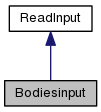
\includegraphics[width=148pt]{class_bodiesinput__inherit__graph}
\end{center}
\end{figure}


Collaboration diagram for Bodiesinput\-:\nopagebreak
\begin{figure}[H]
\begin{center}
\leavevmode
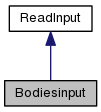
\includegraphics[width=148pt]{class_bodiesinput__coll__graph}
\end{center}
\end{figure}
\subsection*{Public Member Functions}
\begin{DoxyCompactItemize}
\item 
\hyperlink{class_bodiesinput_a978009fcccf310bddf3ecb2261f7b9ed}{Bodiesinput} ()
\item 
\hyperlink{class_bodiesinput_ab478797f356b2d02c7be5a04c5e08d69}{$\sim$\-Bodiesinput} ()
\item 
void \hyperlink{class_bodiesinput_ab4dda6e4b858b9e349b5cc9ba155b4cd}{test\-Print} ()
\item 
vector$<$ \hyperlink{class_body}{Body} $>$ \& \hyperlink{class_bodiesinput_a0526664103347cd11e2b6fc15e8f8e61}{get\-Body\-Data} ()
\end{DoxyCompactItemize}
\subsection*{Protected Member Functions}
\begin{DoxyCompactItemize}
\item 
void \hyperlink{class_bodiesinput_ae7c0a7ee2c02e1ed63658a7d06f257e5}{initialize\-Defaults} ()
\item 
int \hyperlink{class_bodiesinput_abe777be6f9181f1d0f8c5ad523eff6e3}{legal\-Keyword} (string)
\item 
bool \hyperlink{class_bodiesinput_a2bf5785740ebd6e397477e667af16a05}{keyword\-Handler} (int, string, string)
\item 
bool \hyperlink{class_bodiesinput_af735a952cbd5b1a0c5db67c7209ba847}{keyword\-Handler} (int, vector$<$ string $>$, bool)
\item 
void \hyperlink{class_bodiesinput_a752cc5feeefe16345651b8133a132411}{add\-New\-Body} (string)
\end{DoxyCompactItemize}


\subsection{Detailed Description}
This class parses input from file and stores the data appropriately in the \hyperlink{class_body}{Body} object(s). 

\subsection{Constructor \& Destructor Documentation}
\hypertarget{class_bodiesinput_a978009fcccf310bddf3ecb2261f7b9ed}{\index{Bodiesinput@{Bodiesinput}!Bodiesinput@{Bodiesinput}}
\index{Bodiesinput@{Bodiesinput}!Bodiesinput@{Bodiesinput}}
\subsubsection[{Bodiesinput}]{\setlength{\rightskip}{0pt plus 5cm}Bodiesinput\-::\-Bodiesinput (
\begin{DoxyParamCaption}
{}
\end{DoxyParamCaption}
)}}\label{class_bodiesinput_a978009fcccf310bddf3ecb2261f7b9ed}
The default constructor. \hypertarget{class_bodiesinput_ab478797f356b2d02c7be5a04c5e08d69}{\index{Bodiesinput@{Bodiesinput}!$\sim$\-Bodiesinput@{$\sim$\-Bodiesinput}}
\index{$\sim$\-Bodiesinput@{$\sim$\-Bodiesinput}!Bodiesinput@{Bodiesinput}}
\subsubsection[{$\sim$\-Bodiesinput}]{\setlength{\rightskip}{0pt plus 5cm}Bodiesinput\-::$\sim$\-Bodiesinput (
\begin{DoxyParamCaption}
{}
\end{DoxyParamCaption}
)}}\label{class_bodiesinput_ab478797f356b2d02c7be5a04c5e08d69}
The default destructor, nothing happens here. 

\subsection{Member Function Documentation}
\hypertarget{class_bodiesinput_a752cc5feeefe16345651b8133a132411}{\index{Bodiesinput@{Bodiesinput}!add\-New\-Body@{add\-New\-Body}}
\index{add\-New\-Body@{add\-New\-Body}!Bodiesinput@{Bodiesinput}}
\subsubsection[{add\-New\-Body}]{\setlength{\rightskip}{0pt plus 5cm}void Bodiesinput\-::add\-New\-Body (
\begin{DoxyParamCaption}
\item[{string}]{new\-Name}
\end{DoxyParamCaption}
)\hspace{0.3cm}{\ttfamily [protected]}}}\label{class_bodiesinput_a752cc5feeefe16345651b8133a132411}
Adds a new body to the list. 
\begin{DoxyParams}{Parameters}
{\em new\-Name} & The name of the body to be added to the list. \\
\hline
\end{DoxyParams}


Here is the call graph for this function\-:\nopagebreak
\begin{figure}[H]
\begin{center}
\leavevmode
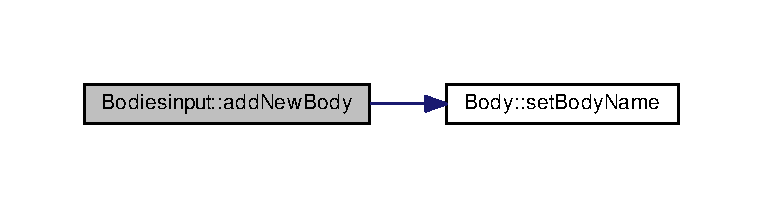
\includegraphics[width=350pt]{class_bodiesinput_a752cc5feeefe16345651b8133a132411_cgraph}
\end{center}
\end{figure}




Here is the caller graph for this function\-:\nopagebreak
\begin{figure}[H]
\begin{center}
\leavevmode
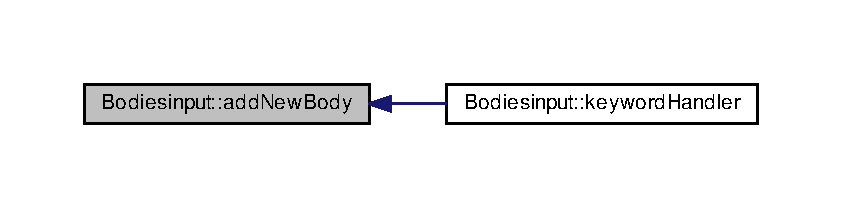
\includegraphics[width=350pt]{class_bodiesinput_a752cc5feeefe16345651b8133a132411_icgraph}
\end{center}
\end{figure}


\hypertarget{class_bodiesinput_a0526664103347cd11e2b6fc15e8f8e61}{\index{Bodiesinput@{Bodiesinput}!get\-Body\-Data@{get\-Body\-Data}}
\index{get\-Body\-Data@{get\-Body\-Data}!Bodiesinput@{Bodiesinput}}
\subsubsection[{get\-Body\-Data}]{\setlength{\rightskip}{0pt plus 5cm}vector$<$ {\bf Body} $>$ \& Bodiesinput\-::get\-Body\-Data (
\begin{DoxyParamCaption}
{}
\end{DoxyParamCaption}
)}}\label{class_bodiesinput_a0526664103347cd11e2b6fc15e8f8e61}
Returns all bodies. \hypertarget{class_bodiesinput_ae7c0a7ee2c02e1ed63658a7d06f257e5}{\index{Bodiesinput@{Bodiesinput}!initialize\-Defaults@{initialize\-Defaults}}
\index{initialize\-Defaults@{initialize\-Defaults}!Bodiesinput@{Bodiesinput}}
\subsubsection[{initialize\-Defaults}]{\setlength{\rightskip}{0pt plus 5cm}void Bodiesinput\-::initialize\-Defaults (
\begin{DoxyParamCaption}
{}
\end{DoxyParamCaption}
)\hspace{0.3cm}{\ttfamily [protected]}, {\ttfamily [virtual]}}}\label{class_bodiesinput_ae7c0a7ee2c02e1ed63658a7d06f257e5}
For future use, does nothing as of now. 

Implements \hyperlink{class_read_input_a4ff2727b876cfd7c01299b08bdd65646}{Read\-Input}.

\hypertarget{class_bodiesinput_a2bf5785740ebd6e397477e667af16a05}{\index{Bodiesinput@{Bodiesinput}!keyword\-Handler@{keyword\-Handler}}
\index{keyword\-Handler@{keyword\-Handler}!Bodiesinput@{Bodiesinput}}
\subsubsection[{keyword\-Handler}]{\setlength{\rightskip}{0pt plus 5cm}bool Bodiesinput\-::keyword\-Handler (
\begin{DoxyParamCaption}
\item[{int}]{key\-Control, }
\item[{string}]{identifier, }
\item[{string}]{val}
\end{DoxyParamCaption}
)\hspace{0.3cm}{\ttfamily [protected]}, {\ttfamily [virtual]}}}\label{class_bodiesinput_a2bf5785740ebd6e397477e667af16a05}
Stores the data if valid keyword according to the legeal\-Keyword function. 
\begin{DoxyParams}{Parameters}
{\em key\-Control} & Indicated which case in switch function to use. \\
\hline
{\em identifier} & The keyword. \\
\hline
{\em val} & The value associated with the keyword. \\
\hline
\end{DoxyParams}
\begin{DoxyReturn}{Returns}
false if not done reading data, true to move onto next keyword in parser. 
\end{DoxyReturn}


Implements \hyperlink{class_read_input_a1d8cb0ef59f265300b682de97513f48d}{Read\-Input}.



Here is the call graph for this function\-:\nopagebreak
\begin{figure}[H]
\begin{center}
\leavevmode
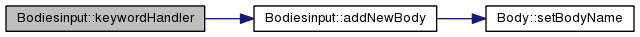
\includegraphics[width=350pt]{class_bodiesinput_a2bf5785740ebd6e397477e667af16a05_cgraph}
\end{center}
\end{figure}


\hypertarget{class_bodiesinput_af735a952cbd5b1a0c5db67c7209ba847}{\index{Bodiesinput@{Bodiesinput}!keyword\-Handler@{keyword\-Handler}}
\index{keyword\-Handler@{keyword\-Handler}!Bodiesinput@{Bodiesinput}}
\subsubsection[{keyword\-Handler}]{\setlength{\rightskip}{0pt plus 5cm}bool Bodiesinput\-::keyword\-Handler (
\begin{DoxyParamCaption}
\item[{int}]{key\-Control, }
\item[{vector$<$ string $>$}]{the\-List\-In, }
\item[{bool}]{is\-Direct}
\end{DoxyParamCaption}
)\hspace{0.3cm}{\ttfamily [protected]}, {\ttfamily [virtual]}}}\label{class_bodiesinput_af735a952cbd5b1a0c5db67c7209ba847}
Stores the list data if valid keyword according to the legeal\-Keyword function. 
\begin{DoxyParams}{Parameters}
{\em key\-Control} & Indicated which case in switch function to use. \\
\hline
{\em the\-List\-In} & List of Values. \\
\hline
{\em is\-Direct} & True if Direct Access List, False if Sequenctial List. \\
\hline
\end{DoxyParams}
\begin{DoxyReturn}{Returns}
false if not done reading data, true to move onto next keyword in parser. 
\end{DoxyReturn}


Implements \hyperlink{class_read_input_afb66a7ff67d0aeb10a3cfa5a4fbc31f8}{Read\-Input}.

\hypertarget{class_bodiesinput_abe777be6f9181f1d0f8c5ad523eff6e3}{\index{Bodiesinput@{Bodiesinput}!legal\-Keyword@{legal\-Keyword}}
\index{legal\-Keyword@{legal\-Keyword}!Bodiesinput@{Bodiesinput}}
\subsubsection[{legal\-Keyword}]{\setlength{\rightskip}{0pt plus 5cm}int Bodiesinput\-::legal\-Keyword (
\begin{DoxyParamCaption}
\item[{string}]{string\-In}
\end{DoxyParamCaption}
)\hspace{0.3cm}{\ttfamily [protected]}, {\ttfamily [virtual]}}}\label{class_bodiesinput_abe777be6f9181f1d0f8c5ad523eff6e3}
Returns int greater than 0 if the keyword is legal, the int returned specifies how to handle data in keyword\-Handler. 
\begin{DoxyParams}{Parameters}
{\em string\-In} & Check if a valid keyword. \\
\hline
\end{DoxyParams}
\begin{DoxyReturn}{Returns}
int value which tells keyword\-Handler how to handle the data. 
\end{DoxyReturn}


Implements \hyperlink{class_read_input_a4c67f10e813686bf635dd4c6bb2c61bc}{Read\-Input}.

\hypertarget{class_bodiesinput_ab4dda6e4b858b9e349b5cc9ba155b4cd}{\index{Bodiesinput@{Bodiesinput}!test\-Print@{test\-Print}}
\index{test\-Print@{test\-Print}!Bodiesinput@{Bodiesinput}}
\subsubsection[{test\-Print}]{\setlength{\rightskip}{0pt plus 5cm}void Bodiesinput\-::test\-Print (
\begin{DoxyParamCaption}
{}
\end{DoxyParamCaption}
)}}\label{class_bodiesinput_ab4dda6e4b858b9e349b5cc9ba155b4cd}
Print to console all data members. 

The documentation for this class was generated from the following files\-:\begin{DoxyCompactItemize}
\item 
/home/nicholas/\-Ship Design/\-Projects/\-D\-M\-S1305 Open\-S\-E\-A/master/200\-\_\-src/bin/ofreq/file\-\_\-reader/bodiesinput.\-h\item 
/home/nicholas/\-Ship Design/\-Projects/\-D\-M\-S1305 Open\-S\-E\-A/master/200\-\_\-src/bin/ofreq/file\-\_\-reader/bodiesinput.\-cpp\end{DoxyCompactItemize}

\hypertarget{class_body}{\section{Body Class Reference}
\label{class_body}\index{Body@{Body}}
}


{\ttfamily \#include $<$body.\-h$>$}

\subsection*{Public Member Functions}
\begin{DoxyCompactItemize}
\item 
\hyperlink{class_body_a7727b0d8c998bbc2942e4c802e31e2eb}{Body} ()
\item 
\hyperlink{class_body_abe1c4da65568cf7978b6247affc461e3}{$\sim$\-Body} ()
\item 
void \hyperlink{class_body_a31b959b6f30e3c9c6ebc3f0a325fec9d}{test\-Print} ()
\item 
void \hyperlink{class_body_a21190f9d796d631202db6caf768beae1}{set\-Body\-Name} (string)
\item 
void \hyperlink{class_body_ac2cb95c1a4d24e6b456db9bfe3e6dea3}{set\-Hydro\-Body\-Name} (string)
\item 
void \hyperlink{class_body_a7bba55a8fd4aea7a17ce7bd5f54d6ab8}{set\-Heading} (double)
\item 
void \hyperlink{class_body_a8165a9147387e4fc34757dab76e11117}{set\-Motion\-Model} (string)
\item 
void \hyperlink{class_body_aaa26153bd320830684e65bbf538b139d}{set\-User\-Active\-Forces} (vector$<$ string $>$)
\item 
void \hyperlink{class_body_aa3b532c91892c7336309df492cad39d6}{set\-User\-Reactive\-Forces} (vector$<$ string $>$)
\item 
void \hyperlink{class_body_af409e4b49b838e118a57a753879685dc}{set\-User\-Cross\-Body\-Forces} (vector$<$ string $>$)
\item 
void \hyperlink{class_body_a34950bfba0878d2488f91a0f5a1ae918}{set\-Hydro\-Active\-Forces} (vector$<$ string $>$)
\item 
void \hyperlink{class_body_ae26fc5ecce5fd1803ce26bf87d1d2a2b}{set\-Hydro\-Reactive\-Forces} (vector$<$ string $>$)
\item 
void \hyperlink{class_body_a47aed2abb4a77b9da93a803f7fdd5e31}{set\-Hydro\-Cross\-Body\-Forces} (vector$<$ string $>$)
\item 
void \hyperlink{class_body_a1bcd87df62f0cdd063c01799c1631ebd}{add\-Linked\-Body} (string)
\item 
void \hyperlink{class_body_a896b660a9d001422f5d2b0b4e6d77b98}{set\-Mass} (double)
\item 
void \hyperlink{class_body_a741a229a3671a7cf3d399a4e5d02596c}{set\-Moment\-X\-X} (double)
\item 
void \hyperlink{class_body_a06cdb969a55ebeff8d83ffcae66ab4ed}{set\-Moment\-Y\-Y} (double)
\item 
void \hyperlink{class_body_a270e3714cad10195b7dadc749727dba7}{set\-Moment\-Z\-Z} (double)
\item 
void \hyperlink{class_body_a24ddd15ae01d27675788658e65fcb199}{set\-Cross\-Moment\-X\-Y} (double)
\item 
void \hyperlink{class_body_a5f75e49f031e7b3dd711dd8e9d25eee8}{set\-Cross\-Moment\-X\-Z} (double)
\item 
void \hyperlink{class_body_ab99551cb3c2183db44ef86304b2e134b}{set\-Cross\-Moment\-Y\-Z} (double)
\item 
void \hyperlink{class_body_aca9af7a0a510f0a1ee9b0b29f7ed0217}{set\-Centroid\-X} (double)
\item 
void \hyperlink{class_body_a86f41f3de49b7e79c2387d92bb124204}{set\-Centroid\-Y} (double)
\item 
void \hyperlink{class_body_ad778b4919794533f12cfb93e818d5759}{set\-Centroid\-Z} (double)
\item 
void \hyperlink{class_body_a38933b2aec94873355dcecc8f8b41db2}{set\-Cross\-Body\-Name} (string)
\item 
string \hyperlink{class_body_ab4340cac445ae26ae751a08c35155386}{get\-Motion\-Model} ()
\item 
string \hyperlink{class_body_aab63febbe35984d8551a188b40ee3c3f}{get\-Body\-Name} ()
\end{DoxyCompactItemize}
\subsection*{Public Attributes}
\begin{DoxyCompactItemize}
\item 
vector$<$ string $>$ \hyperlink{class_body_a76e1e921e0cec08caed125073844c217}{user\-Active\-Forces}
\item 
vector$<$ string $>$ \hyperlink{class_body_af74f87986817f8c5cbd8408b29d04063}{user\-Reactive\-Forces}
\item 
vector$<$ string $>$ \hyperlink{class_body_a0ab89cfc3da49d74fa35ed90a0740e28}{user\-Cross\-Body\-Forces}
\item 
vector$<$ string $>$ \hyperlink{class_body_af307fb84335ee5e795b44595ce63015c}{hydro\-Active\-Forces}
\item 
vector$<$ string $>$ \hyperlink{class_body_a45e72e2a50d93068862b57bf4850a43b}{hydro\-Reactive\-Forces}
\item 
vector$<$ string $>$ \hyperlink{class_body_ad5ab2bc2f00fcb646a27398b0245696d}{hydro\-Cross\-Body\-Forces}
\item 
vector$<$ string $>$ \hyperlink{class_body_aabf9875fae852bd842d4b2b57d25eb73}{linked\-Body}
\item 
string \hyperlink{class_body_aa1ea62768021b84bb1c290c6bfaedbfe}{body\-Name}
\item 
string \hyperlink{class_body_a843782f1874dd366786864d9d3e0d9b7}{hydro\-Body}
\item 
string \hyperlink{class_body_a013a08fbeb1dd82131735dade5faa972}{motion\-Model}
\item 
double \hyperlink{class_body_abeaee44e6bc187426a1012bdaacb6eb4}{mass}
\item 
double \hyperlink{class_body_af29b06cfb14adbd1ad58d10a138a43c4}{moment\-Of\-Inertia\-X\-X}
\item 
double \hyperlink{class_body_adc1f40d6f14c7fea48f261170b8f4746}{moment\-Of\-Inertia\-Y\-Y}
\item 
double \hyperlink{class_body_a6f7c025addc1fd46cf72c18713a9cacf}{moment\-Of\-Inertia\-Z\-Z}
\item 
double \hyperlink{class_body_afd989f0185a85ef68120e88d6564631f}{cross\-Moment\-Of\-Inertia\-X\-Y}
\item 
double \hyperlink{class_body_a15c460e8cc8ae20b2420b379c0a6c760}{cross\-Moment\-Of\-Inertia\-X\-Z}
\item 
double \hyperlink{class_body_a552260d9dc6a203857955df8cc58662a}{cross\-Moment\-Of\-Inertia\-Y\-Z}
\item 
double \hyperlink{class_body_a5dc912a4a096590e90fd681a01ffc708}{centroid\-X}
\item 
double \hyperlink{class_body_aac1b166131421c882d1ec647b740c865}{centroid\-Y}
\item 
double \hyperlink{class_body_a834c22ac029cd86bc72185f027cdf74f}{centroid\-Z}
\item 
double \hyperlink{class_body_afe24a9330df6c053cc4fbbd03d477954}{heading}
\end{DoxyCompactItemize}


\subsection{Detailed Description}
This class holds all of the data for the \hyperlink{class_body}{Body} Input File. 

\subsection{Constructor \& Destructor Documentation}
\hypertarget{class_body_a7727b0d8c998bbc2942e4c802e31e2eb}{\index{Body@{Body}!Body@{Body}}
\index{Body@{Body}!Body@{Body}}
\subsubsection[{Body}]{\setlength{\rightskip}{0pt plus 5cm}Body\-::\-Body (
\begin{DoxyParamCaption}
{}
\end{DoxyParamCaption}
)}}\label{class_body_a7727b0d8c998bbc2942e4c802e31e2eb}
The default constructor \hypertarget{class_body_abe1c4da65568cf7978b6247affc461e3}{\index{Body@{Body}!$\sim$\-Body@{$\sim$\-Body}}
\index{$\sim$\-Body@{$\sim$\-Body}!Body@{Body}}
\subsubsection[{$\sim$\-Body}]{\setlength{\rightskip}{0pt plus 5cm}Body\-::$\sim$\-Body (
\begin{DoxyParamCaption}
{}
\end{DoxyParamCaption}
)}}\label{class_body_abe1c4da65568cf7978b6247affc461e3}
The default destructor, nothing happens here. 

\subsection{Member Function Documentation}
\hypertarget{class_body_a1bcd87df62f0cdd063c01799c1631ebd}{\index{Body@{Body}!add\-Linked\-Body@{add\-Linked\-Body}}
\index{add\-Linked\-Body@{add\-Linked\-Body}!Body@{Body}}
\subsubsection[{add\-Linked\-Body}]{\setlength{\rightskip}{0pt plus 5cm}void Body\-::add\-Linked\-Body (
\begin{DoxyParamCaption}
\item[{string}]{new\-Linked\-Body}
\end{DoxyParamCaption}
)}}\label{class_body_a1bcd87df62f0cdd063c01799c1631ebd}
Adds a linked body. 
\begin{DoxyParams}{Parameters}
{\em new\-Linked\-Body} & The string passed in is added to the linked\-Body vector. \\
\hline
\end{DoxyParams}
\hypertarget{class_body_aab63febbe35984d8551a188b40ee3c3f}{\index{Body@{Body}!get\-Body\-Name@{get\-Body\-Name}}
\index{get\-Body\-Name@{get\-Body\-Name}!Body@{Body}}
\subsubsection[{get\-Body\-Name}]{\setlength{\rightskip}{0pt plus 5cm}string Body\-::get\-Body\-Name (
\begin{DoxyParamCaption}
{}
\end{DoxyParamCaption}
)}}\label{class_body_aab63febbe35984d8551a188b40ee3c3f}
Get the name of the body. \begin{DoxyReturn}{Returns}
The name of the body. 
\end{DoxyReturn}
\hypertarget{class_body_ab4340cac445ae26ae751a08c35155386}{\index{Body@{Body}!get\-Motion\-Model@{get\-Motion\-Model}}
\index{get\-Motion\-Model@{get\-Motion\-Model}!Body@{Body}}
\subsubsection[{get\-Motion\-Model}]{\setlength{\rightskip}{0pt plus 5cm}string Body\-::get\-Motion\-Model (
\begin{DoxyParamCaption}
{}
\end{DoxyParamCaption}
)}}\label{class_body_ab4340cac445ae26ae751a08c35155386}
Get the name of the Motion Model. \begin{DoxyReturn}{Returns}
The string returned is the motion\-Model. 
\end{DoxyReturn}
\hypertarget{class_body_a21190f9d796d631202db6caf768beae1}{\index{Body@{Body}!set\-Body\-Name@{set\-Body\-Name}}
\index{set\-Body\-Name@{set\-Body\-Name}!Body@{Body}}
\subsubsection[{set\-Body\-Name}]{\setlength{\rightskip}{0pt plus 5cm}void Body\-::set\-Body\-Name (
\begin{DoxyParamCaption}
\item[{string}]{new\-Name}
\end{DoxyParamCaption}
)}}\label{class_body_a21190f9d796d631202db6caf768beae1}
Sets the body\-Name. 
\begin{DoxyParams}{Parameters}
{\em new\-Name} & The string passed in sets body\-Name. \\
\hline
\end{DoxyParams}
\hypertarget{class_body_aca9af7a0a510f0a1ee9b0b29f7ed0217}{\index{Body@{Body}!set\-Centroid\-X@{set\-Centroid\-X}}
\index{set\-Centroid\-X@{set\-Centroid\-X}!Body@{Body}}
\subsubsection[{set\-Centroid\-X}]{\setlength{\rightskip}{0pt plus 5cm}void Body\-::set\-Centroid\-X (
\begin{DoxyParamCaption}
\item[{double}]{new\-Cen\-X}
\end{DoxyParamCaption}
)}}\label{class_body_aca9af7a0a510f0a1ee9b0b29f7ed0217}
Sets the Centroid X. 
\begin{DoxyParams}{Parameters}
{\em new\-Cen\-X} & The double passed in sets centroid\-X. \\
\hline
\end{DoxyParams}
\hypertarget{class_body_a86f41f3de49b7e79c2387d92bb124204}{\index{Body@{Body}!set\-Centroid\-Y@{set\-Centroid\-Y}}
\index{set\-Centroid\-Y@{set\-Centroid\-Y}!Body@{Body}}
\subsubsection[{set\-Centroid\-Y}]{\setlength{\rightskip}{0pt plus 5cm}void Body\-::set\-Centroid\-Y (
\begin{DoxyParamCaption}
\item[{double}]{new\-Cen\-Y}
\end{DoxyParamCaption}
)}}\label{class_body_a86f41f3de49b7e79c2387d92bb124204}
Sets the Centroid Y. 
\begin{DoxyParams}{Parameters}
{\em new\-Cen\-Y} & The double passed in sets centroid\-Y. \\
\hline
\end{DoxyParams}
\hypertarget{class_body_ad778b4919794533f12cfb93e818d5759}{\index{Body@{Body}!set\-Centroid\-Z@{set\-Centroid\-Z}}
\index{set\-Centroid\-Z@{set\-Centroid\-Z}!Body@{Body}}
\subsubsection[{set\-Centroid\-Z}]{\setlength{\rightskip}{0pt plus 5cm}void Body\-::set\-Centroid\-Z (
\begin{DoxyParamCaption}
\item[{double}]{new\-Cen\-Z}
\end{DoxyParamCaption}
)}}\label{class_body_ad778b4919794533f12cfb93e818d5759}
Sets the Centroid Z. 
\begin{DoxyParams}{Parameters}
{\em new\-Cen\-Z} & The double passed in sets centroid\-Z. \\
\hline
\end{DoxyParams}
\hypertarget{class_body_a38933b2aec94873355dcecc8f8b41db2}{\index{Body@{Body}!set\-Cross\-Body\-Name@{set\-Cross\-Body\-Name}}
\index{set\-Cross\-Body\-Name@{set\-Cross\-Body\-Name}!Body@{Body}}
\subsubsection[{set\-Cross\-Body\-Name}]{\setlength{\rightskip}{0pt plus 5cm}void Body\-::set\-Cross\-Body\-Name (
\begin{DoxyParamCaption}
\item[{string}]{new\-Name}
\end{DoxyParamCaption}
)}}\label{class_body_a38933b2aec94873355dcecc8f8b41db2}
Adds a cross body name. 
\begin{DoxyParams}{Parameters}
{\em new\-Name} & The string passed in is added to the vector that holds the list of cross body forces. \\
\hline
\end{DoxyParams}
\hypertarget{class_body_a24ddd15ae01d27675788658e65fcb199}{\index{Body@{Body}!set\-Cross\-Moment\-X\-Y@{set\-Cross\-Moment\-X\-Y}}
\index{set\-Cross\-Moment\-X\-Y@{set\-Cross\-Moment\-X\-Y}!Body@{Body}}
\subsubsection[{set\-Cross\-Moment\-X\-Y}]{\setlength{\rightskip}{0pt plus 5cm}void Body\-::set\-Cross\-Moment\-X\-Y (
\begin{DoxyParamCaption}
\item[{double}]{new\-X\-Y}
\end{DoxyParamCaption}
)}}\label{class_body_a24ddd15ae01d27675788658e65fcb199}
Sets the Product of Inertia X\-Y (Ixy) 
\begin{DoxyParams}{Parameters}
{\em new\-X\-Y} & The double passed in sets set\-Cross\-Moment\-X\-Y. \\
\hline
\end{DoxyParams}
\hypertarget{class_body_a5f75e49f031e7b3dd711dd8e9d25eee8}{\index{Body@{Body}!set\-Cross\-Moment\-X\-Z@{set\-Cross\-Moment\-X\-Z}}
\index{set\-Cross\-Moment\-X\-Z@{set\-Cross\-Moment\-X\-Z}!Body@{Body}}
\subsubsection[{set\-Cross\-Moment\-X\-Z}]{\setlength{\rightskip}{0pt plus 5cm}void Body\-::set\-Cross\-Moment\-X\-Z (
\begin{DoxyParamCaption}
\item[{double}]{new\-X\-Z}
\end{DoxyParamCaption}
)}}\label{class_body_a5f75e49f031e7b3dd711dd8e9d25eee8}
Sets the Product of Inertia X\-Z (Ixz) 
\begin{DoxyParams}{Parameters}
{\em new\-X\-Z} & The double passed in sets set\-Cross\-Moment\-X\-Z. \\
\hline
\end{DoxyParams}
\hypertarget{class_body_ab99551cb3c2183db44ef86304b2e134b}{\index{Body@{Body}!set\-Cross\-Moment\-Y\-Z@{set\-Cross\-Moment\-Y\-Z}}
\index{set\-Cross\-Moment\-Y\-Z@{set\-Cross\-Moment\-Y\-Z}!Body@{Body}}
\subsubsection[{set\-Cross\-Moment\-Y\-Z}]{\setlength{\rightskip}{0pt plus 5cm}void Body\-::set\-Cross\-Moment\-Y\-Z (
\begin{DoxyParamCaption}
\item[{double}]{new\-Y\-Z}
\end{DoxyParamCaption}
)}}\label{class_body_ab99551cb3c2183db44ef86304b2e134b}
Sets the Product of Inertia Y\-Z (Iyz) 
\begin{DoxyParams}{Parameters}
{\em new\-Y\-Z} & The double passed in sets set\-Cross\-Moment\-Y\-Z. \\
\hline
\end{DoxyParams}
\hypertarget{class_body_a7bba55a8fd4aea7a17ce7bd5f54d6ab8}{\index{Body@{Body}!set\-Heading@{set\-Heading}}
\index{set\-Heading@{set\-Heading}!Body@{Body}}
\subsubsection[{set\-Heading}]{\setlength{\rightskip}{0pt plus 5cm}void Body\-::set\-Heading (
\begin{DoxyParamCaption}
\item[{double}]{new\-Heading}
\end{DoxyParamCaption}
)}}\label{class_body_a7bba55a8fd4aea7a17ce7bd5f54d6ab8}
Sets the heading. 
\begin{DoxyParams}{Parameters}
{\em new\-Heading} & The double passed in sets the heading. \\
\hline
\end{DoxyParams}
\hypertarget{class_body_a34950bfba0878d2488f91a0f5a1ae918}{\index{Body@{Body}!set\-Hydro\-Active\-Forces@{set\-Hydro\-Active\-Forces}}
\index{set\-Hydro\-Active\-Forces@{set\-Hydro\-Active\-Forces}!Body@{Body}}
\subsubsection[{set\-Hydro\-Active\-Forces}]{\setlength{\rightskip}{0pt plus 5cm}void Body\-::set\-Hydro\-Active\-Forces (
\begin{DoxyParamCaption}
\item[{vector$<$ string $>$}]{new\-Force\-List}
\end{DoxyParamCaption}
)}}\label{class_body_a34950bfba0878d2488f91a0f5a1ae918}
Sets the hydro active forces. 
\begin{DoxyParams}{Parameters}
{\em new\-Force\-List} & The vector of strings sets hydro\-Active\-Forces. \\
\hline
\end{DoxyParams}
\hypertarget{class_body_ac2cb95c1a4d24e6b456db9bfe3e6dea3}{\index{Body@{Body}!set\-Hydro\-Body\-Name@{set\-Hydro\-Body\-Name}}
\index{set\-Hydro\-Body\-Name@{set\-Hydro\-Body\-Name}!Body@{Body}}
\subsubsection[{set\-Hydro\-Body\-Name}]{\setlength{\rightskip}{0pt plus 5cm}void Body\-::set\-Hydro\-Body\-Name (
\begin{DoxyParamCaption}
\item[{string}]{new\-Name}
\end{DoxyParamCaption}
)}}\label{class_body_ac2cb95c1a4d24e6b456db9bfe3e6dea3}
Sets the hydro\-Body. 
\begin{DoxyParams}{Parameters}
{\em new\-Name} & The string passed in sets the hydro\-Body. \\
\hline
\end{DoxyParams}
\hypertarget{class_body_a47aed2abb4a77b9da93a803f7fdd5e31}{\index{Body@{Body}!set\-Hydro\-Cross\-Body\-Forces@{set\-Hydro\-Cross\-Body\-Forces}}
\index{set\-Hydro\-Cross\-Body\-Forces@{set\-Hydro\-Cross\-Body\-Forces}!Body@{Body}}
\subsubsection[{set\-Hydro\-Cross\-Body\-Forces}]{\setlength{\rightskip}{0pt plus 5cm}void Body\-::set\-Hydro\-Cross\-Body\-Forces (
\begin{DoxyParamCaption}
\item[{vector$<$ string $>$}]{new\-Force\-List}
\end{DoxyParamCaption}
)}}\label{class_body_a47aed2abb4a77b9da93a803f7fdd5e31}
Sets the hydro active forces. 
\begin{DoxyParams}{Parameters}
{\em new\-Force\-List} & The vector of strings sets hydro\-Cross\-Body\-Forces. \\
\hline
\end{DoxyParams}
\hypertarget{class_body_ae26fc5ecce5fd1803ce26bf87d1d2a2b}{\index{Body@{Body}!set\-Hydro\-Reactive\-Forces@{set\-Hydro\-Reactive\-Forces}}
\index{set\-Hydro\-Reactive\-Forces@{set\-Hydro\-Reactive\-Forces}!Body@{Body}}
\subsubsection[{set\-Hydro\-Reactive\-Forces}]{\setlength{\rightskip}{0pt plus 5cm}void Body\-::set\-Hydro\-Reactive\-Forces (
\begin{DoxyParamCaption}
\item[{vector$<$ string $>$}]{new\-Force\-List}
\end{DoxyParamCaption}
)}}\label{class_body_ae26fc5ecce5fd1803ce26bf87d1d2a2b}
Sets the hydro reactive forces. 
\begin{DoxyParams}{Parameters}
{\em new\-Force\-List} & The vector of strings sets hydro\-Reactive\-Force. \\
\hline
\end{DoxyParams}
\hypertarget{class_body_a896b660a9d001422f5d2b0b4e6d77b98}{\index{Body@{Body}!set\-Mass@{set\-Mass}}
\index{set\-Mass@{set\-Mass}!Body@{Body}}
\subsubsection[{set\-Mass}]{\setlength{\rightskip}{0pt plus 5cm}void Body\-::set\-Mass (
\begin{DoxyParamCaption}
\item[{double}]{new\-Mass}
\end{DoxyParamCaption}
)}}\label{class_body_a896b660a9d001422f5d2b0b4e6d77b98}
Sets the mass. 
\begin{DoxyParams}{Parameters}
{\em new\-Mass} & The double passed in sets the mass. \\
\hline
\end{DoxyParams}
\hypertarget{class_body_a741a229a3671a7cf3d399a4e5d02596c}{\index{Body@{Body}!set\-Moment\-X\-X@{set\-Moment\-X\-X}}
\index{set\-Moment\-X\-X@{set\-Moment\-X\-X}!Body@{Body}}
\subsubsection[{set\-Moment\-X\-X}]{\setlength{\rightskip}{0pt plus 5cm}void Body\-::set\-Moment\-X\-X (
\begin{DoxyParamCaption}
\item[{double}]{new\-X\-X}
\end{DoxyParamCaption}
)}}\label{class_body_a741a229a3671a7cf3d399a4e5d02596c}
Sets the Moment of Inertia X\-X (Ixx) 
\begin{DoxyParams}{Parameters}
{\em new\-X\-X} & The double passed in sets moment\-Of\-Inertia\-X\-X. \\
\hline
\end{DoxyParams}
\hypertarget{class_body_a06cdb969a55ebeff8d83ffcae66ab4ed}{\index{Body@{Body}!set\-Moment\-Y\-Y@{set\-Moment\-Y\-Y}}
\index{set\-Moment\-Y\-Y@{set\-Moment\-Y\-Y}!Body@{Body}}
\subsubsection[{set\-Moment\-Y\-Y}]{\setlength{\rightskip}{0pt plus 5cm}void Body\-::set\-Moment\-Y\-Y (
\begin{DoxyParamCaption}
\item[{double}]{new\-Y\-Y}
\end{DoxyParamCaption}
)}}\label{class_body_a06cdb969a55ebeff8d83ffcae66ab4ed}
Sets the Moment of Inertia Y\-Y (Iyy) 
\begin{DoxyParams}{Parameters}
{\em new\-Y\-Y} & The double passed in sets moment\-Of\-Inertia\-Y\-Y. \\
\hline
\end{DoxyParams}
\hypertarget{class_body_a270e3714cad10195b7dadc749727dba7}{\index{Body@{Body}!set\-Moment\-Z\-Z@{set\-Moment\-Z\-Z}}
\index{set\-Moment\-Z\-Z@{set\-Moment\-Z\-Z}!Body@{Body}}
\subsubsection[{set\-Moment\-Z\-Z}]{\setlength{\rightskip}{0pt plus 5cm}void Body\-::set\-Moment\-Z\-Z (
\begin{DoxyParamCaption}
\item[{double}]{new\-Z\-Z}
\end{DoxyParamCaption}
)}}\label{class_body_a270e3714cad10195b7dadc749727dba7}
Sets the Moment of Inertia Z\-Z (Izz) 
\begin{DoxyParams}{Parameters}
{\em new\-Z\-Z} & The double passed in sets moment\-Of\-Inertia\-Z\-Z. \\
\hline
\end{DoxyParams}
\hypertarget{class_body_a8165a9147387e4fc34757dab76e11117}{\index{Body@{Body}!set\-Motion\-Model@{set\-Motion\-Model}}
\index{set\-Motion\-Model@{set\-Motion\-Model}!Body@{Body}}
\subsubsection[{set\-Motion\-Model}]{\setlength{\rightskip}{0pt plus 5cm}void Body\-::set\-Motion\-Model (
\begin{DoxyParamCaption}
\item[{string}]{new\-Motion\-Model}
\end{DoxyParamCaption}
)}}\label{class_body_a8165a9147387e4fc34757dab76e11117}
Sets the motion model. 
\begin{DoxyParams}{Parameters}
{\em new\-Motion\-Model} & The string passeed in sets the motion\-Model. \\
\hline
\end{DoxyParams}
\hypertarget{class_body_aaa26153bd320830684e65bbf538b139d}{\index{Body@{Body}!set\-User\-Active\-Forces@{set\-User\-Active\-Forces}}
\index{set\-User\-Active\-Forces@{set\-User\-Active\-Forces}!Body@{Body}}
\subsubsection[{set\-User\-Active\-Forces}]{\setlength{\rightskip}{0pt plus 5cm}void Body\-::set\-User\-Active\-Forces (
\begin{DoxyParamCaption}
\item[{vector$<$ string $>$}]{new\-Force\-List}
\end{DoxyParamCaption}
)}}\label{class_body_aaa26153bd320830684e65bbf538b139d}
Sets the user active forces. 
\begin{DoxyParams}{Parameters}
{\em new\-Force\-List} & The vector of strings sets user\-Active\-Forces. \\
\hline
\end{DoxyParams}
\hypertarget{class_body_af409e4b49b838e118a57a753879685dc}{\index{Body@{Body}!set\-User\-Cross\-Body\-Forces@{set\-User\-Cross\-Body\-Forces}}
\index{set\-User\-Cross\-Body\-Forces@{set\-User\-Cross\-Body\-Forces}!Body@{Body}}
\subsubsection[{set\-User\-Cross\-Body\-Forces}]{\setlength{\rightskip}{0pt plus 5cm}void Body\-::set\-User\-Cross\-Body\-Forces (
\begin{DoxyParamCaption}
\item[{vector$<$ string $>$}]{new\-Cross\-Body\-List}
\end{DoxyParamCaption}
)}}\label{class_body_af409e4b49b838e118a57a753879685dc}
Sets the user cross body forces. 
\begin{DoxyParams}{Parameters}
{\em new\-Cross\-Body\-List} & The vector of strings sets user\-Cross\-Body\-Forces. \\
\hline
\end{DoxyParams}
\hypertarget{class_body_aa3b532c91892c7336309df492cad39d6}{\index{Body@{Body}!set\-User\-Reactive\-Forces@{set\-User\-Reactive\-Forces}}
\index{set\-User\-Reactive\-Forces@{set\-User\-Reactive\-Forces}!Body@{Body}}
\subsubsection[{set\-User\-Reactive\-Forces}]{\setlength{\rightskip}{0pt plus 5cm}void Body\-::set\-User\-Reactive\-Forces (
\begin{DoxyParamCaption}
\item[{vector$<$ string $>$}]{new\-Force\-List}
\end{DoxyParamCaption}
)}}\label{class_body_aa3b532c91892c7336309df492cad39d6}
Sets the user reactive forces. 
\begin{DoxyParams}{Parameters}
{\em new\-Force\-List} & The vector of strings sets user\-Reactive\-Forces. \\
\hline
\end{DoxyParams}
\hypertarget{class_body_a31b959b6f30e3c9c6ebc3f0a325fec9d}{\index{Body@{Body}!test\-Print@{test\-Print}}
\index{test\-Print@{test\-Print}!Body@{Body}}
\subsubsection[{test\-Print}]{\setlength{\rightskip}{0pt plus 5cm}void Body\-::test\-Print (
\begin{DoxyParamCaption}
{}
\end{DoxyParamCaption}
)}}\label{class_body_a31b959b6f30e3c9c6ebc3f0a325fec9d}
Test print to console the values of all data members. 

\subsection{Member Data Documentation}
\hypertarget{class_body_aa1ea62768021b84bb1c290c6bfaedbfe}{\index{Body@{Body}!body\-Name@{body\-Name}}
\index{body\-Name@{body\-Name}!Body@{Body}}
\subsubsection[{body\-Name}]{\setlength{\rightskip}{0pt plus 5cm}string Body\-::body\-Name}}\label{class_body_aa1ea62768021b84bb1c290c6bfaedbfe}
The name of this body object. \hypertarget{class_body_a5dc912a4a096590e90fd681a01ffc708}{\index{Body@{Body}!centroid\-X@{centroid\-X}}
\index{centroid\-X@{centroid\-X}!Body@{Body}}
\subsubsection[{centroid\-X}]{\setlength{\rightskip}{0pt plus 5cm}double Body\-::centroid\-X}}\label{class_body_a5dc912a4a096590e90fd681a01ffc708}
Centroid X. \hypertarget{class_body_aac1b166131421c882d1ec647b740c865}{\index{Body@{Body}!centroid\-Y@{centroid\-Y}}
\index{centroid\-Y@{centroid\-Y}!Body@{Body}}
\subsubsection[{centroid\-Y}]{\setlength{\rightskip}{0pt plus 5cm}double Body\-::centroid\-Y}}\label{class_body_aac1b166131421c882d1ec647b740c865}
Centroid Y. \hypertarget{class_body_a834c22ac029cd86bc72185f027cdf74f}{\index{Body@{Body}!centroid\-Z@{centroid\-Z}}
\index{centroid\-Z@{centroid\-Z}!Body@{Body}}
\subsubsection[{centroid\-Z}]{\setlength{\rightskip}{0pt plus 5cm}double Body\-::centroid\-Z}}\label{class_body_a834c22ac029cd86bc72185f027cdf74f}
Centroid Z. \hypertarget{class_body_afd989f0185a85ef68120e88d6564631f}{\index{Body@{Body}!cross\-Moment\-Of\-Inertia\-X\-Y@{cross\-Moment\-Of\-Inertia\-X\-Y}}
\index{cross\-Moment\-Of\-Inertia\-X\-Y@{cross\-Moment\-Of\-Inertia\-X\-Y}!Body@{Body}}
\subsubsection[{cross\-Moment\-Of\-Inertia\-X\-Y}]{\setlength{\rightskip}{0pt plus 5cm}double Body\-::cross\-Moment\-Of\-Inertia\-X\-Y}}\label{class_body_afd989f0185a85ef68120e88d6564631f}
Product of Inertia X\-Y (Ixy). \hypertarget{class_body_a15c460e8cc8ae20b2420b379c0a6c760}{\index{Body@{Body}!cross\-Moment\-Of\-Inertia\-X\-Z@{cross\-Moment\-Of\-Inertia\-X\-Z}}
\index{cross\-Moment\-Of\-Inertia\-X\-Z@{cross\-Moment\-Of\-Inertia\-X\-Z}!Body@{Body}}
\subsubsection[{cross\-Moment\-Of\-Inertia\-X\-Z}]{\setlength{\rightskip}{0pt plus 5cm}double Body\-::cross\-Moment\-Of\-Inertia\-X\-Z}}\label{class_body_a15c460e8cc8ae20b2420b379c0a6c760}
Product of Inertia X\-Z (Ixz). \hypertarget{class_body_a552260d9dc6a203857955df8cc58662a}{\index{Body@{Body}!cross\-Moment\-Of\-Inertia\-Y\-Z@{cross\-Moment\-Of\-Inertia\-Y\-Z}}
\index{cross\-Moment\-Of\-Inertia\-Y\-Z@{cross\-Moment\-Of\-Inertia\-Y\-Z}!Body@{Body}}
\subsubsection[{cross\-Moment\-Of\-Inertia\-Y\-Z}]{\setlength{\rightskip}{0pt plus 5cm}double Body\-::cross\-Moment\-Of\-Inertia\-Y\-Z}}\label{class_body_a552260d9dc6a203857955df8cc58662a}
Product of Inertia Y\-Z (Iyz). \hypertarget{class_body_afe24a9330df6c053cc4fbbd03d477954}{\index{Body@{Body}!heading@{heading}}
\index{heading@{heading}!Body@{Body}}
\subsubsection[{heading}]{\setlength{\rightskip}{0pt plus 5cm}double Body\-::heading}}\label{class_body_afe24a9330df6c053cc4fbbd03d477954}
Heading. \hypertarget{class_body_af307fb84335ee5e795b44595ce63015c}{\index{Body@{Body}!hydro\-Active\-Forces@{hydro\-Active\-Forces}}
\index{hydro\-Active\-Forces@{hydro\-Active\-Forces}!Body@{Body}}
\subsubsection[{hydro\-Active\-Forces}]{\setlength{\rightskip}{0pt plus 5cm}vector$<$string$>$ Body\-::hydro\-Active\-Forces}}\label{class_body_af307fb84335ee5e795b44595ce63015c}
Holds the hydro active forces. \hypertarget{class_body_a843782f1874dd366786864d9d3e0d9b7}{\index{Body@{Body}!hydro\-Body@{hydro\-Body}}
\index{hydro\-Body@{hydro\-Body}!Body@{Body}}
\subsubsection[{hydro\-Body}]{\setlength{\rightskip}{0pt plus 5cm}string Body\-::hydro\-Body}}\label{class_body_a843782f1874dd366786864d9d3e0d9b7}
The name of this hydro body object. \hypertarget{class_body_ad5ab2bc2f00fcb646a27398b0245696d}{\index{Body@{Body}!hydro\-Cross\-Body\-Forces@{hydro\-Cross\-Body\-Forces}}
\index{hydro\-Cross\-Body\-Forces@{hydro\-Cross\-Body\-Forces}!Body@{Body}}
\subsubsection[{hydro\-Cross\-Body\-Forces}]{\setlength{\rightskip}{0pt plus 5cm}vector$<$string$>$ Body\-::hydro\-Cross\-Body\-Forces}}\label{class_body_ad5ab2bc2f00fcb646a27398b0245696d}
Holds the hydro cross body forces. \hypertarget{class_body_a45e72e2a50d93068862b57bf4850a43b}{\index{Body@{Body}!hydro\-Reactive\-Forces@{hydro\-Reactive\-Forces}}
\index{hydro\-Reactive\-Forces@{hydro\-Reactive\-Forces}!Body@{Body}}
\subsubsection[{hydro\-Reactive\-Forces}]{\setlength{\rightskip}{0pt plus 5cm}vector$<$string$>$ Body\-::hydro\-Reactive\-Forces}}\label{class_body_a45e72e2a50d93068862b57bf4850a43b}
Holds the hydro reactive forces. \hypertarget{class_body_aabf9875fae852bd842d4b2b57d25eb73}{\index{Body@{Body}!linked\-Body@{linked\-Body}}
\index{linked\-Body@{linked\-Body}!Body@{Body}}
\subsubsection[{linked\-Body}]{\setlength{\rightskip}{0pt plus 5cm}vector$<$string$>$ Body\-::linked\-Body}}\label{class_body_aabf9875fae852bd842d4b2b57d25eb73}
Holds a list of the linked bodies. \hypertarget{class_body_abeaee44e6bc187426a1012bdaacb6eb4}{\index{Body@{Body}!mass@{mass}}
\index{mass@{mass}!Body@{Body}}
\subsubsection[{mass}]{\setlength{\rightskip}{0pt plus 5cm}double Body\-::mass}}\label{class_body_abeaee44e6bc187426a1012bdaacb6eb4}
The mass. \hypertarget{class_body_af29b06cfb14adbd1ad58d10a138a43c4}{\index{Body@{Body}!moment\-Of\-Inertia\-X\-X@{moment\-Of\-Inertia\-X\-X}}
\index{moment\-Of\-Inertia\-X\-X@{moment\-Of\-Inertia\-X\-X}!Body@{Body}}
\subsubsection[{moment\-Of\-Inertia\-X\-X}]{\setlength{\rightskip}{0pt plus 5cm}double Body\-::moment\-Of\-Inertia\-X\-X}}\label{class_body_af29b06cfb14adbd1ad58d10a138a43c4}
Moment of Inertia X\-X (Ixx). \hypertarget{class_body_adc1f40d6f14c7fea48f261170b8f4746}{\index{Body@{Body}!moment\-Of\-Inertia\-Y\-Y@{moment\-Of\-Inertia\-Y\-Y}}
\index{moment\-Of\-Inertia\-Y\-Y@{moment\-Of\-Inertia\-Y\-Y}!Body@{Body}}
\subsubsection[{moment\-Of\-Inertia\-Y\-Y}]{\setlength{\rightskip}{0pt plus 5cm}double Body\-::moment\-Of\-Inertia\-Y\-Y}}\label{class_body_adc1f40d6f14c7fea48f261170b8f4746}
Moment of Inertia Y\-Y (Iyy). \hypertarget{class_body_a6f7c025addc1fd46cf72c18713a9cacf}{\index{Body@{Body}!moment\-Of\-Inertia\-Z\-Z@{moment\-Of\-Inertia\-Z\-Z}}
\index{moment\-Of\-Inertia\-Z\-Z@{moment\-Of\-Inertia\-Z\-Z}!Body@{Body}}
\subsubsection[{moment\-Of\-Inertia\-Z\-Z}]{\setlength{\rightskip}{0pt plus 5cm}double Body\-::moment\-Of\-Inertia\-Z\-Z}}\label{class_body_a6f7c025addc1fd46cf72c18713a9cacf}
Moment of Inertia Z\-Z (Izz). \hypertarget{class_body_a013a08fbeb1dd82131735dade5faa972}{\index{Body@{Body}!motion\-Model@{motion\-Model}}
\index{motion\-Model@{motion\-Model}!Body@{Body}}
\subsubsection[{motion\-Model}]{\setlength{\rightskip}{0pt plus 5cm}string Body\-::motion\-Model}}\label{class_body_a013a08fbeb1dd82131735dade5faa972}
The name of the motion model used for this body. \hypertarget{class_body_a76e1e921e0cec08caed125073844c217}{\index{Body@{Body}!user\-Active\-Forces@{user\-Active\-Forces}}
\index{user\-Active\-Forces@{user\-Active\-Forces}!Body@{Body}}
\subsubsection[{user\-Active\-Forces}]{\setlength{\rightskip}{0pt plus 5cm}vector$<$string$>$ Body\-::user\-Active\-Forces}}\label{class_body_a76e1e921e0cec08caed125073844c217}
Holds the user active forces. \hypertarget{class_body_a0ab89cfc3da49d74fa35ed90a0740e28}{\index{Body@{Body}!user\-Cross\-Body\-Forces@{user\-Cross\-Body\-Forces}}
\index{user\-Cross\-Body\-Forces@{user\-Cross\-Body\-Forces}!Body@{Body}}
\subsubsection[{user\-Cross\-Body\-Forces}]{\setlength{\rightskip}{0pt plus 5cm}vector$<$string$>$ Body\-::user\-Cross\-Body\-Forces}}\label{class_body_a0ab89cfc3da49d74fa35ed90a0740e28}
Holds the user cross body forces. \hypertarget{class_body_af74f87986817f8c5cbd8408b29d04063}{\index{Body@{Body}!user\-Reactive\-Forces@{user\-Reactive\-Forces}}
\index{user\-Reactive\-Forces@{user\-Reactive\-Forces}!Body@{Body}}
\subsubsection[{user\-Reactive\-Forces}]{\setlength{\rightskip}{0pt plus 5cm}vector$<$string$>$ Body\-::user\-Reactive\-Forces}}\label{class_body_af74f87986817f8c5cbd8408b29d04063}
Holds the user reactive forces. 

The documentation for this class was generated from the following files\-:\begin{DoxyCompactItemize}
\item 
Visual Studio 2010/\-Projects/o\-Freq Windows V\-S2010/o\-Freq/body.\-h\item 
Visual Studio 2010/\-Projects/o\-Freq Windows V\-S2010/o\-Freq/body.\-cpp\end{DoxyCompactItemize}

\hypertarget{class_body_with_force_matrix}{\section{Body\-With\-Force\-Matrix Class Reference}
\label{class_body_with_force_matrix}\index{Body\-With\-Force\-Matrix@{Body\-With\-Force\-Matrix}}
}
\subsection*{Public Member Functions}
\begin{DoxyCompactItemize}
\item 
\hyperlink{class_body_with_force_matrix_ac3c8391555c45e0a7eab476bf3488ae0}{Body\-With\-Force\-Matrix} ()
\item 
\hyperlink{class_body_with_force_matrix_a075b1ba0f74b27588f3e9affb7b9bb9e}{Body\-With\-Force\-Matrix} (\hyperlink{class_body}{Body}, \hyperlink{class_user_forces}{User\-Forces})
\item 
\hyperlink{class_body_with_force_matrix_a3eef8f497f99e49af7264a49a48a945d}{$\sim$\-Body\-With\-Force\-Matrix} ()
\end{DoxyCompactItemize}
\subsection*{Public Attributes}
\begin{DoxyCompactItemize}
\item 
cx\-\_\-mat \hyperlink{class_body_with_force_matrix_a3b07fb8ac7d58c1ed2b642676e51de6f}{mass\-Matrix}
\item 
vector$<$ \hyperlink{class_reactive_force_matrix}{Reactive\-Force\-Matrix} $>$ \hyperlink{class_body_with_force_matrix_a301fe6541bda12f4786c254688b1b89f}{user\-Reactive\-Force\-Matrix}
\item 
vector$<$ \hyperlink{class_reactive_force_matrix}{Reactive\-Force\-Matrix} $>$ \hyperlink{class_body_with_force_matrix_ad04bf64c3495a2d316f4ede7e6e307d3}{user\-Cross\-Body\-Force\-Matrix}
\item 
vector$<$ cx\-\_\-mat $>$ \hyperlink{class_body_with_force_matrix_aeb11660f006b6e86e8fc691bf55ce346}{user\-Active\-Force\-Matrix}
\item 
vector$<$ \hyperlink{class_reactive_force_matrix}{Reactive\-Force\-Matrix} $>$ \hyperlink{class_body_with_force_matrix_ab9be7a7eb8a4772ca011586590cfcbed}{hydro\-Reactive\-Force\-Matrix}
\item 
vector$<$ \hyperlink{class_reactive_force_matrix}{Reactive\-Force\-Matrix} $>$ \hyperlink{class_body_with_force_matrix_a0fe089e2b9d9bacaf38d8e2e957ee125}{hydro\-Cross\-Body\-Force\-Matrix}
\item 
vector$<$ cx\-\_\-mat $>$ \hyperlink{class_body_with_force_matrix_a8902e9ad82255e0794dff72725928ff9}{hydro\-Active\-Force\-Matrix}
\item 
vector$<$ string $>$ \hyperlink{class_body_with_force_matrix_adff7e3220bdcf4e367a5626afad29572}{user\-Active\-Force}
\item 
vector$<$ string $>$ \hyperlink{class_body_with_force_matrix_ad334068959cd4ad8591c31ff9d16225f}{user\-Reactive\-Force}
\item 
vector$<$ string $>$ \hyperlink{class_body_with_force_matrix_ad97183b090f4f9a1010bcfe028ec55b6}{user\-Cross\-Body\-Forces}
\item 
vector$<$ string $>$ \hyperlink{class_body_with_force_matrix_abab87c2d9bad9c11e526aa35fbe242cb}{hydro\-Active\-Force}
\item 
vector$<$ string $>$ \hyperlink{class_body_with_force_matrix_ade2cce8108c19527e229f960b7bf7cd1}{hydro\-Reactive\-Force}
\item 
vector$<$ string $>$ \hyperlink{class_body_with_force_matrix_ae43f824670c354999843f2cc3e0987c8}{hydro\-Cross\-Body\-Forces}
\end{DoxyCompactItemize}


\subsection{Constructor \& Destructor Documentation}
\hypertarget{class_body_with_force_matrix_ac3c8391555c45e0a7eab476bf3488ae0}{\index{Body\-With\-Force\-Matrix@{Body\-With\-Force\-Matrix}!Body\-With\-Force\-Matrix@{Body\-With\-Force\-Matrix}}
\index{Body\-With\-Force\-Matrix@{Body\-With\-Force\-Matrix}!BodyWithForceMatrix@{Body\-With\-Force\-Matrix}}
\subsubsection[{Body\-With\-Force\-Matrix}]{\setlength{\rightskip}{0pt plus 5cm}Body\-With\-Force\-Matrix\-::\-Body\-With\-Force\-Matrix (
\begin{DoxyParamCaption}
{}
\end{DoxyParamCaption}
)}}\label{class_body_with_force_matrix_ac3c8391555c45e0a7eab476bf3488ae0}
The default constructor. \hypertarget{class_body_with_force_matrix_a075b1ba0f74b27588f3e9affb7b9bb9e}{\index{Body\-With\-Force\-Matrix@{Body\-With\-Force\-Matrix}!Body\-With\-Force\-Matrix@{Body\-With\-Force\-Matrix}}
\index{Body\-With\-Force\-Matrix@{Body\-With\-Force\-Matrix}!BodyWithForceMatrix@{Body\-With\-Force\-Matrix}}
\subsubsection[{Body\-With\-Force\-Matrix}]{\setlength{\rightskip}{0pt plus 5cm}Body\-With\-Force\-Matrix\-::\-Body\-With\-Force\-Matrix (
\begin{DoxyParamCaption}
\item[{{\bf Body}}]{body\-In, }
\item[{{\bf User\-Forces}}]{user\-Forces\-In}
\end{DoxyParamCaption}
)}}\label{class_body_with_force_matrix_a075b1ba0f74b27588f3e9affb7b9bb9e}
The Constructor. Not used. 
\begin{DoxyParams}{Parameters}
{\em body\-In} & The body. \\
\hline
{\em The} & forces list. \\
\hline
\end{DoxyParams}
\hypertarget{class_body_with_force_matrix_a3eef8f497f99e49af7264a49a48a945d}{\index{Body\-With\-Force\-Matrix@{Body\-With\-Force\-Matrix}!$\sim$\-Body\-With\-Force\-Matrix@{$\sim$\-Body\-With\-Force\-Matrix}}
\index{$\sim$\-Body\-With\-Force\-Matrix@{$\sim$\-Body\-With\-Force\-Matrix}!BodyWithForceMatrix@{Body\-With\-Force\-Matrix}}
\subsubsection[{$\sim$\-Body\-With\-Force\-Matrix}]{\setlength{\rightskip}{0pt plus 5cm}Body\-With\-Force\-Matrix\-::$\sim$\-Body\-With\-Force\-Matrix (
\begin{DoxyParamCaption}
{}
\end{DoxyParamCaption}
)}}\label{class_body_with_force_matrix_a3eef8f497f99e49af7264a49a48a945d}
The default destructor, nothing happens here. 

\subsection{Member Data Documentation}
\hypertarget{class_body_with_force_matrix_abab87c2d9bad9c11e526aa35fbe242cb}{\index{Body\-With\-Force\-Matrix@{Body\-With\-Force\-Matrix}!hydro\-Active\-Force@{hydro\-Active\-Force}}
\index{hydro\-Active\-Force@{hydro\-Active\-Force}!BodyWithForceMatrix@{Body\-With\-Force\-Matrix}}
\subsubsection[{hydro\-Active\-Force}]{\setlength{\rightskip}{0pt plus 5cm}vector$<$string$>$ Body\-With\-Force\-Matrix\-::hydro\-Active\-Force}}\label{class_body_with_force_matrix_abab87c2d9bad9c11e526aa35fbe242cb}
The name of the hydro active forces in the matrices list. \hypertarget{class_body_with_force_matrix_a8902e9ad82255e0794dff72725928ff9}{\index{Body\-With\-Force\-Matrix@{Body\-With\-Force\-Matrix}!hydro\-Active\-Force\-Matrix@{hydro\-Active\-Force\-Matrix}}
\index{hydro\-Active\-Force\-Matrix@{hydro\-Active\-Force\-Matrix}!BodyWithForceMatrix@{Body\-With\-Force\-Matrix}}
\subsubsection[{hydro\-Active\-Force\-Matrix}]{\setlength{\rightskip}{0pt plus 5cm}vector$<$cx\-\_\-mat$>$ Body\-With\-Force\-Matrix\-::hydro\-Active\-Force\-Matrix}}\label{class_body_with_force_matrix_a8902e9ad82255e0794dff72725928ff9}
List of hydro active force matrices. \hypertarget{class_body_with_force_matrix_a0fe089e2b9d9bacaf38d8e2e957ee125}{\index{Body\-With\-Force\-Matrix@{Body\-With\-Force\-Matrix}!hydro\-Cross\-Body\-Force\-Matrix@{hydro\-Cross\-Body\-Force\-Matrix}}
\index{hydro\-Cross\-Body\-Force\-Matrix@{hydro\-Cross\-Body\-Force\-Matrix}!BodyWithForceMatrix@{Body\-With\-Force\-Matrix}}
\subsubsection[{hydro\-Cross\-Body\-Force\-Matrix}]{\setlength{\rightskip}{0pt plus 5cm}vector$<${\bf Reactive\-Force\-Matrix}$>$ Body\-With\-Force\-Matrix\-::hydro\-Cross\-Body\-Force\-Matrix}}\label{class_body_with_force_matrix_a0fe089e2b9d9bacaf38d8e2e957ee125}
List of hydro cross body force matrices. \hypertarget{class_body_with_force_matrix_ae43f824670c354999843f2cc3e0987c8}{\index{Body\-With\-Force\-Matrix@{Body\-With\-Force\-Matrix}!hydro\-Cross\-Body\-Forces@{hydro\-Cross\-Body\-Forces}}
\index{hydro\-Cross\-Body\-Forces@{hydro\-Cross\-Body\-Forces}!BodyWithForceMatrix@{Body\-With\-Force\-Matrix}}
\subsubsection[{hydro\-Cross\-Body\-Forces}]{\setlength{\rightskip}{0pt plus 5cm}vector$<$string$>$ Body\-With\-Force\-Matrix\-::hydro\-Cross\-Body\-Forces}}\label{class_body_with_force_matrix_ae43f824670c354999843f2cc3e0987c8}
The name of the hydro cross body forces in the matrices list. \hypertarget{class_body_with_force_matrix_ade2cce8108c19527e229f960b7bf7cd1}{\index{Body\-With\-Force\-Matrix@{Body\-With\-Force\-Matrix}!hydro\-Reactive\-Force@{hydro\-Reactive\-Force}}
\index{hydro\-Reactive\-Force@{hydro\-Reactive\-Force}!BodyWithForceMatrix@{Body\-With\-Force\-Matrix}}
\subsubsection[{hydro\-Reactive\-Force}]{\setlength{\rightskip}{0pt plus 5cm}vector$<$string$>$ Body\-With\-Force\-Matrix\-::hydro\-Reactive\-Force}}\label{class_body_with_force_matrix_ade2cce8108c19527e229f960b7bf7cd1}
The name of the hydro reactive forces in the matrices list. \hypertarget{class_body_with_force_matrix_ab9be7a7eb8a4772ca011586590cfcbed}{\index{Body\-With\-Force\-Matrix@{Body\-With\-Force\-Matrix}!hydro\-Reactive\-Force\-Matrix@{hydro\-Reactive\-Force\-Matrix}}
\index{hydro\-Reactive\-Force\-Matrix@{hydro\-Reactive\-Force\-Matrix}!BodyWithForceMatrix@{Body\-With\-Force\-Matrix}}
\subsubsection[{hydro\-Reactive\-Force\-Matrix}]{\setlength{\rightskip}{0pt plus 5cm}vector$<${\bf Reactive\-Force\-Matrix}$>$ Body\-With\-Force\-Matrix\-::hydro\-Reactive\-Force\-Matrix}}\label{class_body_with_force_matrix_ab9be7a7eb8a4772ca011586590cfcbed}
List of hydro reactive force matrices. \hypertarget{class_body_with_force_matrix_a3b07fb8ac7d58c1ed2b642676e51de6f}{\index{Body\-With\-Force\-Matrix@{Body\-With\-Force\-Matrix}!mass\-Matrix@{mass\-Matrix}}
\index{mass\-Matrix@{mass\-Matrix}!BodyWithForceMatrix@{Body\-With\-Force\-Matrix}}
\subsubsection[{mass\-Matrix}]{\setlength{\rightskip}{0pt plus 5cm}cx\-\_\-mat Body\-With\-Force\-Matrix\-::mass\-Matrix}}\label{class_body_with_force_matrix_a3b07fb8ac7d58c1ed2b642676e51de6f}
The Mass Matrix. \hypertarget{class_body_with_force_matrix_adff7e3220bdcf4e367a5626afad29572}{\index{Body\-With\-Force\-Matrix@{Body\-With\-Force\-Matrix}!user\-Active\-Force@{user\-Active\-Force}}
\index{user\-Active\-Force@{user\-Active\-Force}!BodyWithForceMatrix@{Body\-With\-Force\-Matrix}}
\subsubsection[{user\-Active\-Force}]{\setlength{\rightskip}{0pt plus 5cm}vector$<$string$>$ Body\-With\-Force\-Matrix\-::user\-Active\-Force}}\label{class_body_with_force_matrix_adff7e3220bdcf4e367a5626afad29572}
The name of the user active forces in the matrices list. \hypertarget{class_body_with_force_matrix_aeb11660f006b6e86e8fc691bf55ce346}{\index{Body\-With\-Force\-Matrix@{Body\-With\-Force\-Matrix}!user\-Active\-Force\-Matrix@{user\-Active\-Force\-Matrix}}
\index{user\-Active\-Force\-Matrix@{user\-Active\-Force\-Matrix}!BodyWithForceMatrix@{Body\-With\-Force\-Matrix}}
\subsubsection[{user\-Active\-Force\-Matrix}]{\setlength{\rightskip}{0pt plus 5cm}vector$<$cx\-\_\-mat$>$ Body\-With\-Force\-Matrix\-::user\-Active\-Force\-Matrix}}\label{class_body_with_force_matrix_aeb11660f006b6e86e8fc691bf55ce346}
List of user active force matrices. \hypertarget{class_body_with_force_matrix_ad04bf64c3495a2d316f4ede7e6e307d3}{\index{Body\-With\-Force\-Matrix@{Body\-With\-Force\-Matrix}!user\-Cross\-Body\-Force\-Matrix@{user\-Cross\-Body\-Force\-Matrix}}
\index{user\-Cross\-Body\-Force\-Matrix@{user\-Cross\-Body\-Force\-Matrix}!BodyWithForceMatrix@{Body\-With\-Force\-Matrix}}
\subsubsection[{user\-Cross\-Body\-Force\-Matrix}]{\setlength{\rightskip}{0pt plus 5cm}vector$<${\bf Reactive\-Force\-Matrix}$>$ Body\-With\-Force\-Matrix\-::user\-Cross\-Body\-Force\-Matrix}}\label{class_body_with_force_matrix_ad04bf64c3495a2d316f4ede7e6e307d3}
List of user cross body force matrices. \hypertarget{class_body_with_force_matrix_ad97183b090f4f9a1010bcfe028ec55b6}{\index{Body\-With\-Force\-Matrix@{Body\-With\-Force\-Matrix}!user\-Cross\-Body\-Forces@{user\-Cross\-Body\-Forces}}
\index{user\-Cross\-Body\-Forces@{user\-Cross\-Body\-Forces}!BodyWithForceMatrix@{Body\-With\-Force\-Matrix}}
\subsubsection[{user\-Cross\-Body\-Forces}]{\setlength{\rightskip}{0pt plus 5cm}vector$<$string$>$ Body\-With\-Force\-Matrix\-::user\-Cross\-Body\-Forces}}\label{class_body_with_force_matrix_ad97183b090f4f9a1010bcfe028ec55b6}
The name of the user cross body forces in the matrices list. \hypertarget{class_body_with_force_matrix_ad334068959cd4ad8591c31ff9d16225f}{\index{Body\-With\-Force\-Matrix@{Body\-With\-Force\-Matrix}!user\-Reactive\-Force@{user\-Reactive\-Force}}
\index{user\-Reactive\-Force@{user\-Reactive\-Force}!BodyWithForceMatrix@{Body\-With\-Force\-Matrix}}
\subsubsection[{user\-Reactive\-Force}]{\setlength{\rightskip}{0pt plus 5cm}vector$<$string$>$ Body\-With\-Force\-Matrix\-::user\-Reactive\-Force}}\label{class_body_with_force_matrix_ad334068959cd4ad8591c31ff9d16225f}
The name of the user reactive forces in the matrices list. \hypertarget{class_body_with_force_matrix_a301fe6541bda12f4786c254688b1b89f}{\index{Body\-With\-Force\-Matrix@{Body\-With\-Force\-Matrix}!user\-Reactive\-Force\-Matrix@{user\-Reactive\-Force\-Matrix}}
\index{user\-Reactive\-Force\-Matrix@{user\-Reactive\-Force\-Matrix}!BodyWithForceMatrix@{Body\-With\-Force\-Matrix}}
\subsubsection[{user\-Reactive\-Force\-Matrix}]{\setlength{\rightskip}{0pt plus 5cm}vector$<${\bf Reactive\-Force\-Matrix}$>$ Body\-With\-Force\-Matrix\-::user\-Reactive\-Force\-Matrix}}\label{class_body_with_force_matrix_a301fe6541bda12f4786c254688b1b89f}
List of user reactive force matrices. 

The documentation for this class was generated from the following files\-:\begin{DoxyCompactItemize}
\item 
Visual Studio 2010/\-Projects/o\-Freq Windows V\-S2010/o\-Freq/bodywithforcematrix.\-h\item 
Visual Studio 2010/\-Projects/o\-Freq Windows V\-S2010/o\-Freq/bodywithforcematrix.\-cpp\end{DoxyCompactItemize}

\hypertarget{class_body_with_solution}{\section{Body\-With\-Solution Class Reference}
\label{class_body_with_solution}\index{Body\-With\-Solution@{Body\-With\-Solution}}
}


{\ttfamily \#include $<$bodywithsolution.\-h$>$}

\subsection*{Public Member Functions}
\begin{DoxyCompactItemize}
\item 
\hyperlink{class_body_with_solution_a6f05c16f0cf4aa726bb60fd3e3b0af1b}{Body\-With\-Solution} (string)
\item 
\hyperlink{class_body_with_solution_ae923a12ef7a43de3667d2370a450e60e}{$\sim$\-Body\-With\-Solution} ()
\end{DoxyCompactItemize}
\subsection*{Public Attributes}
\begin{DoxyCompactItemize}
\item 
string \hyperlink{class_body_with_solution_ad7d65251341438956aba237632a65850}{body\-Name}
\item 
vector$<$ cx\-\_\-mat $>$ \hyperlink{class_body_with_solution_ab137fb3c24fe281c9375146d2e170667}{solution\-Matrix}
\end{DoxyCompactItemize}


\subsection{Detailed Description}
This class holds data to identify a body by name and its solutions. 

\subsection{Constructor \& Destructor Documentation}
\hypertarget{class_body_with_solution_a6f05c16f0cf4aa726bb60fd3e3b0af1b}{\index{Body\-With\-Solution@{Body\-With\-Solution}!Body\-With\-Solution@{Body\-With\-Solution}}
\index{Body\-With\-Solution@{Body\-With\-Solution}!BodyWithSolution@{Body\-With\-Solution}}
\subsubsection[{Body\-With\-Solution}]{\setlength{\rightskip}{0pt plus 5cm}Body\-With\-Solution\-::\-Body\-With\-Solution (
\begin{DoxyParamCaption}
\item[{string}]{name\-In}
\end{DoxyParamCaption}
)}}\label{class_body_with_solution_a6f05c16f0cf4aa726bb60fd3e3b0af1b}
This constructor creates a \hyperlink{class_body_with_solution}{Body\-With\-Solution} object and sets its name to the body it holds data for. 
\begin{DoxyParams}{Parameters}
{\em name\-In} & The string passed in sets the body\-Name of this object. \\
\hline
\end{DoxyParams}
\hypertarget{class_body_with_solution_ae923a12ef7a43de3667d2370a450e60e}{\index{Body\-With\-Solution@{Body\-With\-Solution}!$\sim$\-Body\-With\-Solution@{$\sim$\-Body\-With\-Solution}}
\index{$\sim$\-Body\-With\-Solution@{$\sim$\-Body\-With\-Solution}!BodyWithSolution@{Body\-With\-Solution}}
\subsubsection[{$\sim$\-Body\-With\-Solution}]{\setlength{\rightskip}{0pt plus 5cm}Body\-With\-Solution\-::$\sim$\-Body\-With\-Solution (
\begin{DoxyParamCaption}
{}
\end{DoxyParamCaption}
)}}\label{class_body_with_solution_ae923a12ef7a43de3667d2370a450e60e}
The destructor. Nothing happens here. 

\subsection{Member Data Documentation}
\hypertarget{class_body_with_solution_ad7d65251341438956aba237632a65850}{\index{Body\-With\-Solution@{Body\-With\-Solution}!body\-Name@{body\-Name}}
\index{body\-Name@{body\-Name}!BodyWithSolution@{Body\-With\-Solution}}
\subsubsection[{body\-Name}]{\setlength{\rightskip}{0pt plus 5cm}string Body\-With\-Solution\-::body\-Name}}\label{class_body_with_solution_ad7d65251341438956aba237632a65850}
The name of the body this object represents. \hypertarget{class_body_with_solution_ab137fb3c24fe281c9375146d2e170667}{\index{Body\-With\-Solution@{Body\-With\-Solution}!solution\-Matrix@{solution\-Matrix}}
\index{solution\-Matrix@{solution\-Matrix}!BodyWithSolution@{Body\-With\-Solution}}
\subsubsection[{solution\-Matrix}]{\setlength{\rightskip}{0pt plus 5cm}vector$<$cx\-\_\-mat$>$ Body\-With\-Solution\-::solution\-Matrix}}\label{class_body_with_solution_ab137fb3c24fe281c9375146d2e170667}
Each entry in this vector holds a matrix of complex$<$double$>$ which represents a solution for each frequency 

The documentation for this class was generated from the following files\-:\begin{DoxyCompactItemize}
\item 
Visual Studio 2010/\-Projects/o\-Freq Windows V\-S2010/o\-Freq/bodywithsolution.\-h\item 
Visual Studio 2010/\-Projects/o\-Freq Windows V\-S2010/o\-Freq/bodywithsolution.\-cpp\end{DoxyCompactItemize}

\hypertarget{class_control_input}{\section{Control\-Input Class Reference}
\label{class_control_input}\index{Control\-Input@{Control\-Input}}
}


{\ttfamily \#include $<$controlinput.\-h$>$}



Inheritance diagram for Control\-Input\-:\nopagebreak
\begin{figure}[H]
\begin{center}
\leavevmode
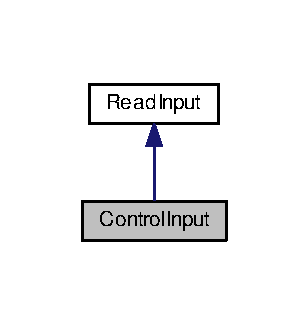
\includegraphics[width=148pt]{class_control_input__inherit__graph}
\end{center}
\end{figure}


Collaboration diagram for Control\-Input\-:\nopagebreak
\begin{figure}[H]
\begin{center}
\leavevmode
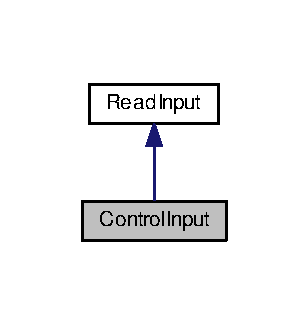
\includegraphics[width=148pt]{class_control_input__coll__graph}
\end{center}
\end{figure}
\subsection*{Public Member Functions}
\begin{DoxyCompactItemize}
\item 
\hyperlink{class_control_input_a50dc4cde4f6410238119971b6934c63a}{Control\-Input} ()
\item 
\hyperlink{class_control_input_aa35022d7c6edbfef7150eb4db594ba58}{$\sim$\-Control\-Input} ()
\item 
void \hyperlink{class_control_input_a2f95d64805ed477f78bf778bb786b30b}{test\-Print} ()
\item 
vector$<$ double $>$ \hyperlink{class_control_input_a3febc929e09306f21f484249c89dbc80}{get\-Wave\-Frequencies} ()
\item 
vector$<$ double $>$ \hyperlink{class_control_input_a2e80de357be6fe5112add0f5066c6328}{get\-Wave\-Directions} ()
\end{DoxyCompactItemize}
\subsection*{Protected Member Functions}
\begin{DoxyCompactItemize}
\item 
void \hyperlink{class_control_input_af15fe8b88a0e7f496c7fd0d4795ff900}{initialize\-Defaults} ()
\item 
int \hyperlink{class_control_input_af7295a9ba455debb812f0e1d4a647820}{legal\-Keyword} (string)
\item 
bool \hyperlink{class_control_input_acb4fb4c1d2a2453e3b8986e44e096f63}{keyword\-Handler} (int, string, string)
\item 
bool \hyperlink{class_control_input_a33b353c2d8f4316d1543059a319faba7}{keyword\-Handler} (int, vector$<$ string $>$, bool)
\end{DoxyCompactItemize}


\subsection{Detailed Description}
This class parses input from file and stores the data appropriately in the \hyperlink{class_system}{System} object. 

\subsection{Constructor \& Destructor Documentation}
\hypertarget{class_control_input_a50dc4cde4f6410238119971b6934c63a}{\index{Control\-Input@{Control\-Input}!Control\-Input@{Control\-Input}}
\index{Control\-Input@{Control\-Input}!ControlInput@{Control\-Input}}
\subsubsection[{Control\-Input}]{\setlength{\rightskip}{0pt plus 5cm}Control\-Input\-::\-Control\-Input (
\begin{DoxyParamCaption}
{}
\end{DoxyParamCaption}
)}}\label{class_control_input_a50dc4cde4f6410238119971b6934c63a}
The default constructor. 

Here is the call graph for this function\-:\nopagebreak
\begin{figure}[H]
\begin{center}
\leavevmode
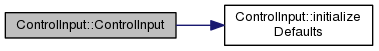
\includegraphics[width=350pt]{class_control_input_a50dc4cde4f6410238119971b6934c63a_cgraph}
\end{center}
\end{figure}


\hypertarget{class_control_input_aa35022d7c6edbfef7150eb4db594ba58}{\index{Control\-Input@{Control\-Input}!$\sim$\-Control\-Input@{$\sim$\-Control\-Input}}
\index{$\sim$\-Control\-Input@{$\sim$\-Control\-Input}!ControlInput@{Control\-Input}}
\subsubsection[{$\sim$\-Control\-Input}]{\setlength{\rightskip}{0pt plus 5cm}Control\-Input\-::$\sim$\-Control\-Input (
\begin{DoxyParamCaption}
{}
\end{DoxyParamCaption}
)}}\label{class_control_input_aa35022d7c6edbfef7150eb4db594ba58}
The default destructor, nothing happens here. 

\subsection{Member Function Documentation}
\hypertarget{class_control_input_a2e80de357be6fe5112add0f5066c6328}{\index{Control\-Input@{Control\-Input}!get\-Wave\-Directions@{get\-Wave\-Directions}}
\index{get\-Wave\-Directions@{get\-Wave\-Directions}!ControlInput@{Control\-Input}}
\subsubsection[{get\-Wave\-Directions}]{\setlength{\rightskip}{0pt plus 5cm}vector$<$ double $>$ Control\-Input\-::get\-Wave\-Directions (
\begin{DoxyParamCaption}
{}
\end{DoxyParamCaption}
)}}\label{class_control_input_a2e80de357be6fe5112add0f5066c6328}
Get function to retrieve wave directions. \begin{DoxyReturn}{Returns}
the list of wave directions. 
\end{DoxyReturn}


Here is the call graph for this function\-:\nopagebreak
\begin{figure}[H]
\begin{center}
\leavevmode
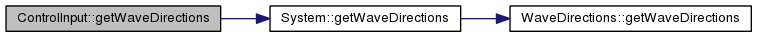
\includegraphics[width=350pt]{class_control_input_a2e80de357be6fe5112add0f5066c6328_cgraph}
\end{center}
\end{figure}


\hypertarget{class_control_input_a3febc929e09306f21f484249c89dbc80}{\index{Control\-Input@{Control\-Input}!get\-Wave\-Frequencies@{get\-Wave\-Frequencies}}
\index{get\-Wave\-Frequencies@{get\-Wave\-Frequencies}!ControlInput@{Control\-Input}}
\subsubsection[{get\-Wave\-Frequencies}]{\setlength{\rightskip}{0pt plus 5cm}vector$<$ double $>$ Control\-Input\-::get\-Wave\-Frequencies (
\begin{DoxyParamCaption}
{}
\end{DoxyParamCaption}
)}}\label{class_control_input_a3febc929e09306f21f484249c89dbc80}
Get function to retrieve wave frequencies. \begin{DoxyReturn}{Returns}
the list of wave frequencies. 
\end{DoxyReturn}


Here is the call graph for this function\-:\nopagebreak
\begin{figure}[H]
\begin{center}
\leavevmode
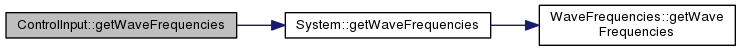
\includegraphics[width=350pt]{class_control_input_a3febc929e09306f21f484249c89dbc80_cgraph}
\end{center}
\end{figure}


\hypertarget{class_control_input_af15fe8b88a0e7f496c7fd0d4795ff900}{\index{Control\-Input@{Control\-Input}!initialize\-Defaults@{initialize\-Defaults}}
\index{initialize\-Defaults@{initialize\-Defaults}!ControlInput@{Control\-Input}}
\subsubsection[{initialize\-Defaults}]{\setlength{\rightskip}{0pt plus 5cm}void Control\-Input\-::initialize\-Defaults (
\begin{DoxyParamCaption}
{}
\end{DoxyParamCaption}
)\hspace{0.3cm}{\ttfamily [protected]}, {\ttfamily [virtual]}}}\label{class_control_input_af15fe8b88a0e7f496c7fd0d4795ff900}
For future use, does nothing as of now. 

Implements \hyperlink{class_read_input_a4ff2727b876cfd7c01299b08bdd65646}{Read\-Input}.



Here is the caller graph for this function\-:\nopagebreak
\begin{figure}[H]
\begin{center}
\leavevmode
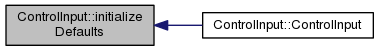
\includegraphics[width=350pt]{class_control_input_af15fe8b88a0e7f496c7fd0d4795ff900_icgraph}
\end{center}
\end{figure}


\hypertarget{class_control_input_acb4fb4c1d2a2453e3b8986e44e096f63}{\index{Control\-Input@{Control\-Input}!keyword\-Handler@{keyword\-Handler}}
\index{keyword\-Handler@{keyword\-Handler}!ControlInput@{Control\-Input}}
\subsubsection[{keyword\-Handler}]{\setlength{\rightskip}{0pt plus 5cm}bool Control\-Input\-::keyword\-Handler (
\begin{DoxyParamCaption}
\item[{int}]{key\-Control, }
\item[{string}]{identifier, }
\item[{string}]{val}
\end{DoxyParamCaption}
)\hspace{0.3cm}{\ttfamily [protected]}, {\ttfamily [virtual]}}}\label{class_control_input_acb4fb4c1d2a2453e3b8986e44e096f63}
Stores the data if valid keyword according to the legeal\-Keyword function. 
\begin{DoxyParams}{Parameters}
{\em key\-Control} & Indicated which case in switch function to use. \\
\hline
{\em identifier} & The keyword. \\
\hline
{\em val} & The value associated with the keyword. \\
\hline
\end{DoxyParams}
\begin{DoxyReturn}{Returns}
false if not done reading data, true to move onto next keyword in parser. 
\end{DoxyReturn}


Implements \hyperlink{class_read_input_a1d8cb0ef59f265300b682de97513f48d}{Read\-Input}.



Here is the call graph for this function\-:\nopagebreak
\begin{figure}[H]
\begin{center}
\leavevmode
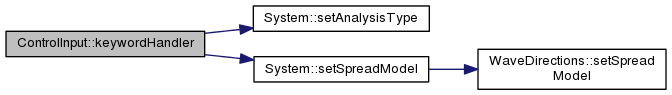
\includegraphics[width=350pt]{class_control_input_acb4fb4c1d2a2453e3b8986e44e096f63_cgraph}
\end{center}
\end{figure}


\hypertarget{class_control_input_a33b353c2d8f4316d1543059a319faba7}{\index{Control\-Input@{Control\-Input}!keyword\-Handler@{keyword\-Handler}}
\index{keyword\-Handler@{keyword\-Handler}!ControlInput@{Control\-Input}}
\subsubsection[{keyword\-Handler}]{\setlength{\rightskip}{0pt plus 5cm}bool Control\-Input\-::keyword\-Handler (
\begin{DoxyParamCaption}
\item[{int}]{key\-Control, }
\item[{vector$<$ string $>$}]{the\-List\-In, }
\item[{bool}]{is\-Direct}
\end{DoxyParamCaption}
)\hspace{0.3cm}{\ttfamily [protected]}, {\ttfamily [virtual]}}}\label{class_control_input_a33b353c2d8f4316d1543059a319faba7}
Stores the list data if valid keyword according to the legeal\-Keyword function. 
\begin{DoxyParams}{Parameters}
{\em key\-Control} & Indicated which case in switch function to use. \\
\hline
{\em the\-List\-In} & List of Values. \\
\hline
{\em is\-Direct} & True if Direct Access List, False if Sequenctial List. \\
\hline
\end{DoxyParams}
\begin{DoxyReturn}{Returns}
false if not done reading data, true to move onto next keyword in parser. 
\end{DoxyReturn}


Implements \hyperlink{class_read_input_afb66a7ff67d0aeb10a3cfa5a4fbc31f8}{Read\-Input}.



Here is the call graph for this function\-:\nopagebreak
\begin{figure}[H]
\begin{center}
\leavevmode
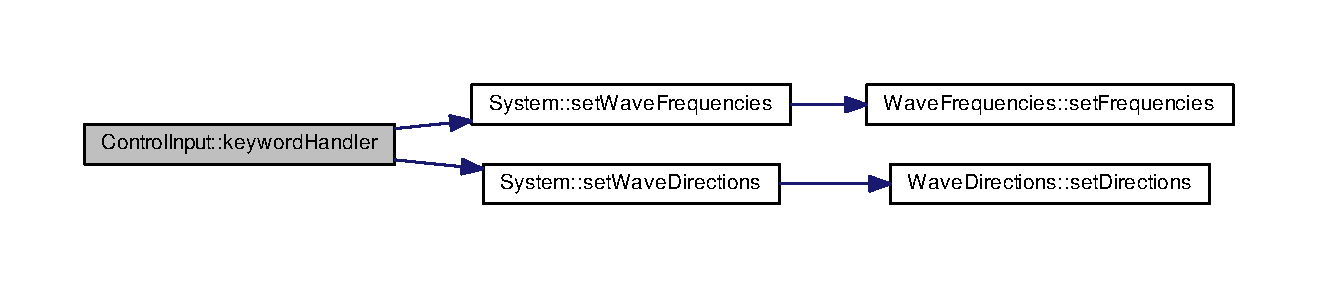
\includegraphics[width=350pt]{class_control_input_a33b353c2d8f4316d1543059a319faba7_cgraph}
\end{center}
\end{figure}


\hypertarget{class_control_input_af7295a9ba455debb812f0e1d4a647820}{\index{Control\-Input@{Control\-Input}!legal\-Keyword@{legal\-Keyword}}
\index{legal\-Keyword@{legal\-Keyword}!ControlInput@{Control\-Input}}
\subsubsection[{legal\-Keyword}]{\setlength{\rightskip}{0pt plus 5cm}int Control\-Input\-::legal\-Keyword (
\begin{DoxyParamCaption}
\item[{string}]{string\-In}
\end{DoxyParamCaption}
)\hspace{0.3cm}{\ttfamily [protected]}, {\ttfamily [virtual]}}}\label{class_control_input_af7295a9ba455debb812f0e1d4a647820}
Returns int greater than 0 if the keyword is legal, the int returned specifies how to handle data in keyword\-Handler. 
\begin{DoxyParams}{Parameters}
{\em string\-In} & Check if a valid keyword. \\
\hline
\end{DoxyParams}
\begin{DoxyReturn}{Returns}
int value which tells keyword\-Handler how to handle the data. 
\end{DoxyReturn}


Implements \hyperlink{class_read_input_a4c67f10e813686bf635dd4c6bb2c61bc}{Read\-Input}.

\hypertarget{class_control_input_a2f95d64805ed477f78bf778bb786b30b}{\index{Control\-Input@{Control\-Input}!test\-Print@{test\-Print}}
\index{test\-Print@{test\-Print}!ControlInput@{Control\-Input}}
\subsubsection[{test\-Print}]{\setlength{\rightskip}{0pt plus 5cm}void Control\-Input\-::test\-Print (
\begin{DoxyParamCaption}
{}
\end{DoxyParamCaption}
)}}\label{class_control_input_a2f95d64805ed477f78bf778bb786b30b}
Print to console all data members. 

Here is the call graph for this function\-:\nopagebreak
\begin{figure}[H]
\begin{center}
\leavevmode
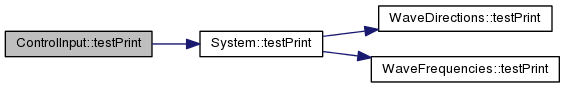
\includegraphics[width=350pt]{class_control_input_a2f95d64805ed477f78bf778bb786b30b_cgraph}
\end{center}
\end{figure}




The documentation for this class was generated from the following files\-:\begin{DoxyCompactItemize}
\item 
/home/nicholas/\-Ship Design/\-Projects/\-D\-M\-S1305 Open\-S\-E\-A/master/200\-\_\-src/bin/ofreq/file\-\_\-reader/controlinput.\-h\item 
/home/nicholas/\-Ship Design/\-Projects/\-D\-M\-S1305 Open\-S\-E\-A/master/200\-\_\-src/bin/ofreq/file\-\_\-reader/controlinput.\-cpp\end{DoxyCompactItemize}

\hypertarget{class_data_input}{\section{Data\-Input Class Reference}
\label{class_data_input}\index{Data\-Input@{Data\-Input}}
}


{\ttfamily \#include $<$datainput.\-h$>$}



Inheritance diagram for Data\-Input\-:\nopagebreak
\begin{figure}[H]
\begin{center}
\leavevmode
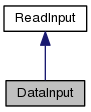
\includegraphics[width=140pt]{class_data_input__inherit__graph}
\end{center}
\end{figure}


Collaboration diagram for Data\-Input\-:\nopagebreak
\begin{figure}[H]
\begin{center}
\leavevmode
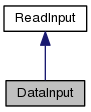
\includegraphics[width=140pt]{class_data_input__coll__graph}
\end{center}
\end{figure}
\subsection*{Public Member Functions}
\begin{DoxyCompactItemize}
\item 
\hyperlink{class_data_input_af2e87fe631ff367c6ef8fa428f3367c4}{Data\-Input} ()
\item 
\hyperlink{class_data_input_a526be3b7b6daeb510ababe0da5222cca}{$\sim$\-Data\-Input} ()
\item 
void \hyperlink{class_data_input_aab1accef9d6147402c2426300656dd3b}{test\-Print} ()
\end{DoxyCompactItemize}
\subsection*{Protected Member Functions}
\begin{DoxyCompactItemize}
\item 
void \hyperlink{class_data_input_a991d4d493aaeaff9d631565b9a49d2ce}{initialize\-Defaults} ()
\item 
int \hyperlink{class_data_input_ae3ca24179103da6e38b99842b9fc1000}{legal\-Keyword} (string)
\item 
bool \hyperlink{class_data_input_a80075c8e86436e00c89d891ce0be57a8}{keyword\-Handler} (int, string, string)
\item 
bool \hyperlink{class_data_input_a70d0380171a30a659a6c7868f2573c92}{keyword\-Handler} (int, vector$<$ string $>$, bool)
\end{DoxyCompactItemize}


\subsection{Detailed Description}
This class parses input from file and stores the data as a list for hyddro file locations. 

\subsection{Constructor \& Destructor Documentation}
\hypertarget{class_data_input_af2e87fe631ff367c6ef8fa428f3367c4}{\index{Data\-Input@{Data\-Input}!Data\-Input@{Data\-Input}}
\index{Data\-Input@{Data\-Input}!DataInput@{Data\-Input}}
\subsubsection[{Data\-Input}]{\setlength{\rightskip}{0pt plus 5cm}Data\-Input\-::\-Data\-Input (
\begin{DoxyParamCaption}
{}
\end{DoxyParamCaption}
)}}\label{class_data_input_af2e87fe631ff367c6ef8fa428f3367c4}
The default constructor. \hypertarget{class_data_input_a526be3b7b6daeb510ababe0da5222cca}{\index{Data\-Input@{Data\-Input}!$\sim$\-Data\-Input@{$\sim$\-Data\-Input}}
\index{$\sim$\-Data\-Input@{$\sim$\-Data\-Input}!DataInput@{Data\-Input}}
\subsubsection[{$\sim$\-Data\-Input}]{\setlength{\rightskip}{0pt plus 5cm}Data\-Input\-::$\sim$\-Data\-Input (
\begin{DoxyParamCaption}
{}
\end{DoxyParamCaption}
)}}\label{class_data_input_a526be3b7b6daeb510ababe0da5222cca}
The default destructor, nothing happens here. 

\subsection{Member Function Documentation}
\hypertarget{class_data_input_a991d4d493aaeaff9d631565b9a49d2ce}{\index{Data\-Input@{Data\-Input}!initialize\-Defaults@{initialize\-Defaults}}
\index{initialize\-Defaults@{initialize\-Defaults}!DataInput@{Data\-Input}}
\subsubsection[{initialize\-Defaults}]{\setlength{\rightskip}{0pt plus 5cm}void Data\-Input\-::initialize\-Defaults (
\begin{DoxyParamCaption}
{}
\end{DoxyParamCaption}
)\hspace{0.3cm}{\ttfamily [protected]}, {\ttfamily [virtual]}}}\label{class_data_input_a991d4d493aaeaff9d631565b9a49d2ce}
For future use, does nothing as of now. 

Implements \hyperlink{class_read_input_a4ff2727b876cfd7c01299b08bdd65646}{Read\-Input}.

\hypertarget{class_data_input_a80075c8e86436e00c89d891ce0be57a8}{\index{Data\-Input@{Data\-Input}!keyword\-Handler@{keyword\-Handler}}
\index{keyword\-Handler@{keyword\-Handler}!DataInput@{Data\-Input}}
\subsubsection[{keyword\-Handler}]{\setlength{\rightskip}{0pt plus 5cm}bool Data\-Input\-::keyword\-Handler (
\begin{DoxyParamCaption}
\item[{int}]{key\-Control, }
\item[{string}]{identifier, }
\item[{string}]{val}
\end{DoxyParamCaption}
)\hspace{0.3cm}{\ttfamily [protected]}, {\ttfamily [virtual]}}}\label{class_data_input_a80075c8e86436e00c89d891ce0be57a8}
Stores the data if valid keyword according to the legeal\-Keyword function. 
\begin{DoxyParams}{Parameters}
{\em key\-Control} & Indicated which case in switch function to use. \\
\hline
{\em identifier} & The keyword. \\
\hline
{\em val} & The value associated with the keyword. \\
\hline
\end{DoxyParams}
\begin{DoxyReturn}{Returns}
false if not done reading data, true to move onto next keyword in parser. 
\end{DoxyReturn}


Implements \hyperlink{class_read_input_a1d8cb0ef59f265300b682de97513f48d}{Read\-Input}.

\hypertarget{class_data_input_a70d0380171a30a659a6c7868f2573c92}{\index{Data\-Input@{Data\-Input}!keyword\-Handler@{keyword\-Handler}}
\index{keyword\-Handler@{keyword\-Handler}!DataInput@{Data\-Input}}
\subsubsection[{keyword\-Handler}]{\setlength{\rightskip}{0pt plus 5cm}bool Data\-Input\-::keyword\-Handler (
\begin{DoxyParamCaption}
\item[{int}]{key\-Control, }
\item[{vector$<$ string $>$}]{the\-List\-In, }
\item[{bool}]{is\-Direct}
\end{DoxyParamCaption}
)\hspace{0.3cm}{\ttfamily [protected]}, {\ttfamily [virtual]}}}\label{class_data_input_a70d0380171a30a659a6c7868f2573c92}
Stores the list data if valid keyword according to the legeal\-Keyword function. 
\begin{DoxyParams}{Parameters}
{\em key\-Control} & Indicated which case in switch function to use. \\
\hline
{\em the\-List\-In} & List of Values. \\
\hline
{\em is\-Direct} & True if Direct Access List, False if Sequenctial List. \\
\hline
\end{DoxyParams}
\begin{DoxyReturn}{Returns}
false if not done reading data, true to move onto next keyword in parser. 
\end{DoxyReturn}


Implements \hyperlink{class_read_input_afb66a7ff67d0aeb10a3cfa5a4fbc31f8}{Read\-Input}.

\hypertarget{class_data_input_ae3ca24179103da6e38b99842b9fc1000}{\index{Data\-Input@{Data\-Input}!legal\-Keyword@{legal\-Keyword}}
\index{legal\-Keyword@{legal\-Keyword}!DataInput@{Data\-Input}}
\subsubsection[{legal\-Keyword}]{\setlength{\rightskip}{0pt plus 5cm}int Data\-Input\-::legal\-Keyword (
\begin{DoxyParamCaption}
\item[{string}]{string\-In}
\end{DoxyParamCaption}
)\hspace{0.3cm}{\ttfamily [protected]}, {\ttfamily [virtual]}}}\label{class_data_input_ae3ca24179103da6e38b99842b9fc1000}
Returns int greater than 0 if the keyword is legal, the int returned specifies how to handle data in keyword\-Handler. 
\begin{DoxyParams}{Parameters}
{\em string\-In} & Check if a valid keyword. \\
\hline
\end{DoxyParams}
\begin{DoxyReturn}{Returns}
int value which tells keyword\-Handler how to handle the data. 
\end{DoxyReturn}


Implements \hyperlink{class_read_input_a4c67f10e813686bf635dd4c6bb2c61bc}{Read\-Input}.

\hypertarget{class_data_input_aab1accef9d6147402c2426300656dd3b}{\index{Data\-Input@{Data\-Input}!test\-Print@{test\-Print}}
\index{test\-Print@{test\-Print}!DataInput@{Data\-Input}}
\subsubsection[{test\-Print}]{\setlength{\rightskip}{0pt plus 5cm}void Data\-Input\-::test\-Print (
\begin{DoxyParamCaption}
{}
\end{DoxyParamCaption}
)}}\label{class_data_input_aab1accef9d6147402c2426300656dd3b}
Print to console all data members. 

The documentation for this class was generated from the following files\-:\begin{DoxyCompactItemize}
\item 
/home/nicholas/\-Ship Design/\-Projects/\-D\-M\-S1305 Open\-S\-E\-A/master/200\-\_\-src/bin/ofreq/file\-\_\-reader/datainput.\-h\item 
/home/nicholas/\-Ship Design/\-Projects/\-D\-M\-S1305 Open\-S\-E\-A/master/200\-\_\-src/bin/ofreq/file\-\_\-reader/datainput.\-cpp\end{DoxyCompactItemize}

\hypertarget{class_derivative}{\section{Derivative Class Reference}
\label{class_derivative}\index{Derivative@{Derivative}}
}


{\ttfamily \#include $<$forcederivative.\-h$>$}

\subsection*{Public Member Functions}
\begin{DoxyCompactItemize}
\item 
\hyperlink{class_derivative_adc03ec3ad150bc0de66a3e7200cd368f}{Derivative} ()
\item 
\hyperlink{class_derivative_a7fc4ee53f460dfb98b3db2e9c9830cf9}{$\sim$\-Derivative} ()
\item 
void \hyperlink{class_derivative_afe00a18765c0d70c3232a41f5ac663dd}{test\-Print} ()
\item 
int \hyperlink{class_derivative_ac95af6fb993314a578b3f0d3cd57a9cc}{get\-Equation\-List\-Size} ()
\end{DoxyCompactItemize}
\subsection*{Public Attributes}
\begin{DoxyCompactItemize}
\item 
\hyperlink{class_equation}{Equation} \hyperlink{class_derivative_a183278e468ffc4d3313968a01c6770ea}{equation\-List} \mbox{[}M\-A\-X\-\_\-\-E\-Q\-U\-A\-T\-I\-O\-N\-S\mbox{]}
\end{DoxyCompactItemize}


\subsection{Detailed Description}
This class holds data for a derivative. 

\subsection{Constructor \& Destructor Documentation}
\hypertarget{class_derivative_adc03ec3ad150bc0de66a3e7200cd368f}{\index{Derivative@{Derivative}!Derivative@{Derivative}}
\index{Derivative@{Derivative}!Derivative@{Derivative}}
\subsubsection[{Derivative}]{\setlength{\rightskip}{0pt plus 5cm}Derivative\-::\-Derivative (
\begin{DoxyParamCaption}
{}
\end{DoxyParamCaption}
)}}\label{class_derivative_adc03ec3ad150bc0de66a3e7200cd368f}
This default constructor creates a \hyperlink{class_body}{Body} object. \hypertarget{class_derivative_a7fc4ee53f460dfb98b3db2e9c9830cf9}{\index{Derivative@{Derivative}!$\sim$\-Derivative@{$\sim$\-Derivative}}
\index{$\sim$\-Derivative@{$\sim$\-Derivative}!Derivative@{Derivative}}
\subsubsection[{$\sim$\-Derivative}]{\setlength{\rightskip}{0pt plus 5cm}Derivative\-::$\sim$\-Derivative (
\begin{DoxyParamCaption}
{}
\end{DoxyParamCaption}
)}}\label{class_derivative_a7fc4ee53f460dfb98b3db2e9c9830cf9}
The default destructor, nothing happens here. 

\subsection{Member Function Documentation}
\hypertarget{class_derivative_ac95af6fb993314a578b3f0d3cd57a9cc}{\index{Derivative@{Derivative}!get\-Equation\-List\-Size@{get\-Equation\-List\-Size}}
\index{get\-Equation\-List\-Size@{get\-Equation\-List\-Size}!Derivative@{Derivative}}
\subsubsection[{get\-Equation\-List\-Size}]{\setlength{\rightskip}{0pt plus 5cm}int Derivative\-::get\-Equation\-List\-Size (
\begin{DoxyParamCaption}
{}
\end{DoxyParamCaption}
)}}\label{class_derivative_ac95af6fb993314a578b3f0d3cd57a9cc}
Retrieve the size of the equation list. \begin{DoxyReturn}{Returns}
The size of the equation list. 
\end{DoxyReturn}
\hypertarget{class_derivative_afe00a18765c0d70c3232a41f5ac663dd}{\index{Derivative@{Derivative}!test\-Print@{test\-Print}}
\index{test\-Print@{test\-Print}!Derivative@{Derivative}}
\subsubsection[{test\-Print}]{\setlength{\rightskip}{0pt plus 5cm}void Derivative\-::test\-Print (
\begin{DoxyParamCaption}
{}
\end{DoxyParamCaption}
)}}\label{class_derivative_afe00a18765c0d70c3232a41f5ac663dd}
Test print to console the values of all data members. 

\subsection{Member Data Documentation}
\hypertarget{class_derivative_a183278e468ffc4d3313968a01c6770ea}{\index{Derivative@{Derivative}!equation\-List@{equation\-List}}
\index{equation\-List@{equation\-List}!Derivative@{Derivative}}
\subsubsection[{equation\-List}]{\setlength{\rightskip}{0pt plus 5cm}{\bf Equation} Derivative\-::equation\-List\mbox{[}M\-A\-X\-\_\-\-E\-Q\-U\-A\-T\-I\-O\-N\-S\mbox{]}}}\label{class_derivative_a183278e468ffc4d3313968a01c6770ea}
The list of equations. 

The documentation for this class was generated from the following files\-:\begin{DoxyCompactItemize}
\item 
Visual Studio 2010/\-Projects/o\-Freq Windows V\-S2010/o\-Freq/forcederivative.\-h\item 
Visual Studio 2010/\-Projects/o\-Freq Windows V\-S2010/o\-Freq/forcederivative.\-cpp\end{DoxyCompactItemize}

\hypertarget{class_equation}{\section{Equation Class Reference}
\label{class_equation}\index{Equation@{Equation}}
}


{\ttfamily \#include $<$equation.\-h$>$}

\subsection*{Public Member Functions}
\begin{DoxyCompactItemize}
\item 
\hyperlink{class_equation_a68511fc719250ed80f86c50de9136733}{Equation} ()
\item 
\hyperlink{class_equation_a37fec641aec75302c37590d191421790}{Equation} (int Index\-In)
\begin{DoxyCompactList}\small\item\em Constructor with setting the data index. \end{DoxyCompactList}\item 
\hyperlink{class_equation_a097243d0dfd608330fc91f115a0d15bb}{$\sim$\-Equation} ()
\item 
void \hyperlink{class_equation_af6c9148998a4abe47f4a4215c51ce3c8}{test\-Print} ()
\item 
vector$<$ double $>$ \& \hyperlink{class_equation_abe2b02e37a07bddaf1040d2d24c3564c}{Coefficients} ()
\begin{DoxyCompactList}\small\item\em Direct access to the list of coefficients. \end{DoxyCompactList}\item 
double \hyperlink{class_equation_a6aa77458d50e80de2a31708756c7925b}{get\-Coefficient} (int number)
\begin{DoxyCompactList}\small\item\em Get the coefficient at the specified number. \end{DoxyCompactList}\item 
void \hyperlink{class_equation_a96dd6f24624703a1ff3ffb4d19a76582}{set\-Coefficient} (int number, double coeff\-In)
\begin{DoxyCompactList}\small\item\em Set the coefficient value at the specified index number. \end{DoxyCompactList}\item 
int \hyperlink{class_equation_abb01745ac8c816354d72ee529d2bddc0}{get\-Coefficient\-List\-Size} ()
\item 
void \hyperlink{class_equation_aa9e40c1cc6fb3cb030e9956663025a87}{set\-Data\-Index} (int index)
\begin{DoxyCompactList}\small\item\em Set the index number of any equation data that should be retrieved. \end{DoxyCompactList}\item 
int \hyperlink{class_equation_ac5fd13eba76ddbbf4813823fad4166e2}{get\-Data\-Index} ()
\begin{DoxyCompactList}\small\item\em Get the index number of any equation data that should be retrieved. \end{DoxyCompactList}\item 
int \& \hyperlink{class_equation_ad3c7c4766cf4b17eaf4f07e0792f012a}{Data\-Index} ()
\begin{DoxyCompactList}\small\item\em Exposed access to the data access variable. \end{DoxyCompactList}\end{DoxyCompactItemize}


\subsection{Detailed Description}
This class holds data for an equation. 

\subsection{Constructor \& Destructor Documentation}
\hypertarget{class_equation_a68511fc719250ed80f86c50de9136733}{\index{Equation@{Equation}!Equation@{Equation}}
\index{Equation@{Equation}!Equation@{Equation}}
\subsubsection[{Equation}]{\setlength{\rightskip}{0pt plus 5cm}Equation\-::\-Equation (
\begin{DoxyParamCaption}
{}
\end{DoxyParamCaption}
)}}\label{class_equation_a68511fc719250ed80f86c50de9136733}
This default constructor. 

Here is the caller graph for this function\-:\nopagebreak
\begin{figure}[H]
\begin{center}
\leavevmode
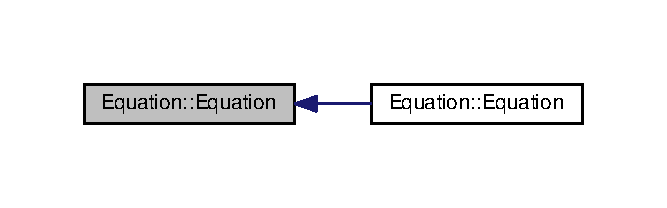
\includegraphics[width=320pt]{class_equation_a68511fc719250ed80f86c50de9136733_icgraph}
\end{center}
\end{figure}


\hypertarget{class_equation_a37fec641aec75302c37590d191421790}{\index{Equation@{Equation}!Equation@{Equation}}
\index{Equation@{Equation}!Equation@{Equation}}
\subsubsection[{Equation}]{\setlength{\rightskip}{0pt plus 5cm}Equation\-::\-Equation (
\begin{DoxyParamCaption}
\item[{int}]{Index\-In}
\end{DoxyParamCaption}
)}}\label{class_equation_a37fec641aec75302c37590d191421790}


Constructor with setting the data index. 

Constructor with setting the data index. 
\begin{DoxyParams}{Parameters}
{\em Index\-In} & The integer specifying the data index number. \\
\hline
\end{DoxyParams}


Here is the call graph for this function\-:\nopagebreak
\begin{figure}[H]
\begin{center}
\leavevmode
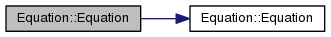
\includegraphics[width=320pt]{class_equation_a37fec641aec75302c37590d191421790_cgraph}
\end{center}
\end{figure}


\hypertarget{class_equation_a097243d0dfd608330fc91f115a0d15bb}{\index{Equation@{Equation}!$\sim$\-Equation@{$\sim$\-Equation}}
\index{$\sim$\-Equation@{$\sim$\-Equation}!Equation@{Equation}}
\subsubsection[{$\sim$\-Equation}]{\setlength{\rightskip}{0pt plus 5cm}Equation\-::$\sim$\-Equation (
\begin{DoxyParamCaption}
{}
\end{DoxyParamCaption}
)}}\label{class_equation_a097243d0dfd608330fc91f115a0d15bb}
The default destructor, nothing happens here. 

\subsection{Member Function Documentation}
\hypertarget{class_equation_abe2b02e37a07bddaf1040d2d24c3564c}{\index{Equation@{Equation}!Coefficients@{Coefficients}}
\index{Coefficients@{Coefficients}!Equation@{Equation}}
\subsubsection[{Coefficients}]{\setlength{\rightskip}{0pt plus 5cm}vector$<$ double $>$ \& Equation\-::\-Coefficients (
\begin{DoxyParamCaption}
{}
\end{DoxyParamCaption}
)}}\label{class_equation_abe2b02e37a07bddaf1040d2d24c3564c}


Direct access to the list of coefficients. 

\begin{DoxyReturn}{Returns}
Pointer to the list of coefficients. 
\end{DoxyReturn}
\hypertarget{class_equation_ad3c7c4766cf4b17eaf4f07e0792f012a}{\index{Equation@{Equation}!Data\-Index@{Data\-Index}}
\index{Data\-Index@{Data\-Index}!Equation@{Equation}}
\subsubsection[{Data\-Index}]{\setlength{\rightskip}{0pt plus 5cm}int \& Equation\-::\-Data\-Index (
\begin{DoxyParamCaption}
{}
\end{DoxyParamCaption}
)}}\label{class_equation_ad3c7c4766cf4b17eaf4f07e0792f012a}


Exposed access to the data access variable. 

\begin{DoxyReturn}{Returns}
Returns the data access variable. Return passed by reference. 
\end{DoxyReturn}
\hypertarget{class_equation_a6aa77458d50e80de2a31708756c7925b}{\index{Equation@{Equation}!get\-Coefficient@{get\-Coefficient}}
\index{get\-Coefficient@{get\-Coefficient}!Equation@{Equation}}
\subsubsection[{get\-Coefficient}]{\setlength{\rightskip}{0pt plus 5cm}double Equation\-::get\-Coefficient (
\begin{DoxyParamCaption}
\item[{int}]{number}
\end{DoxyParamCaption}
)}}\label{class_equation_a6aa77458d50e80de2a31708756c7925b}


Get the coefficient at the specified number. 


\begin{DoxyParams}{Parameters}
{\em number} & The index number of the coefficient to retrieve. \\
\hline
\end{DoxyParams}
\begin{DoxyReturn}{Returns}
Returns a double precision floating point number of the coefficient at the index specified by number. 
\end{DoxyReturn}
\hypertarget{class_equation_abb01745ac8c816354d72ee529d2bddc0}{\index{Equation@{Equation}!get\-Coefficient\-List\-Size@{get\-Coefficient\-List\-Size}}
\index{get\-Coefficient\-List\-Size@{get\-Coefficient\-List\-Size}!Equation@{Equation}}
\subsubsection[{get\-Coefficient\-List\-Size}]{\setlength{\rightskip}{0pt plus 5cm}int Equation\-::get\-Coefficient\-List\-Size (
\begin{DoxyParamCaption}
{}
\end{DoxyParamCaption}
)}}\label{class_equation_abb01745ac8c816354d72ee529d2bddc0}
Retrieve the size of the coefficient list. \begin{DoxyReturn}{Returns}
The size of the coefficient list. 
\end{DoxyReturn}
\hypertarget{class_equation_ac5fd13eba76ddbbf4813823fad4166e2}{\index{Equation@{Equation}!get\-Data\-Index@{get\-Data\-Index}}
\index{get\-Data\-Index@{get\-Data\-Index}!Equation@{Equation}}
\subsubsection[{get\-Data\-Index}]{\setlength{\rightskip}{0pt plus 5cm}int Equation\-::get\-Data\-Index (
\begin{DoxyParamCaption}
{}
\end{DoxyParamCaption}
)}}\label{class_equation_ac5fd13eba76ddbbf4813823fad4166e2}


Get the index number of any equation data that should be retrieved. 

Get the index number of any equation data that should be retrieved. Because the first six values in the index are reserved for 6\-D\-O\-F, it is necessary that equation objects should be able to specify their index as something other than their place in a containing vector. The default initialization value for this is -\/1, which indicates the index is not set. Any number less than zero indicates the index is not set. 
\begin{DoxyParams}{Parameters}
{\em index} & Integer. The index number that should be retrieved. Any number less than zero indicates the index is not set. \\
\hline
\end{DoxyParams}
\hypertarget{class_equation_a96dd6f24624703a1ff3ffb4d19a76582}{\index{Equation@{Equation}!set\-Coefficient@{set\-Coefficient}}
\index{set\-Coefficient@{set\-Coefficient}!Equation@{Equation}}
\subsubsection[{set\-Coefficient}]{\setlength{\rightskip}{0pt plus 5cm}void Equation\-::set\-Coefficient (
\begin{DoxyParamCaption}
\item[{int}]{number, }
\item[{double}]{coeff\-In}
\end{DoxyParamCaption}
)}}\label{class_equation_a96dd6f24624703a1ff3ffb4d19a76582}


Set the coefficient value at the specified index number. 

Set the coefficient value at the specified index number. 
\begin{DoxyParams}{Parameters}
{\em number} & Integer. The index number of the coefficient to set. \\
\hline
{\em coeff\-In} & Double precision floating number. The value of the coefficient to set at the specified index. \\
\hline
\end{DoxyParams}
\hypertarget{class_equation_aa9e40c1cc6fb3cb030e9956663025a87}{\index{Equation@{Equation}!set\-Data\-Index@{set\-Data\-Index}}
\index{set\-Data\-Index@{set\-Data\-Index}!Equation@{Equation}}
\subsubsection[{set\-Data\-Index}]{\setlength{\rightskip}{0pt plus 5cm}void Equation\-::set\-Data\-Index (
\begin{DoxyParamCaption}
\item[{int}]{index}
\end{DoxyParamCaption}
)}}\label{class_equation_aa9e40c1cc6fb3cb030e9956663025a87}


Set the index number of any equation data that should be retrieved. 

Set the index number of any equation data that should be retrieved. Because the first six values in the index are reserved for 6\-D\-O\-F, it is necessary that equation objects should be able to specify their index as something other than their place in a containing vector. The default initialization value for this is -\/1, which indicates the index is not set. Any number less than zero indicates the index is not set. 
\begin{DoxyParams}{Parameters}
{\em index} & The index number that should be set. Any number less than zero indicates the index is not set. \\
\hline
\end{DoxyParams}
\hypertarget{class_equation_af6c9148998a4abe47f4a4215c51ce3c8}{\index{Equation@{Equation}!test\-Print@{test\-Print}}
\index{test\-Print@{test\-Print}!Equation@{Equation}}
\subsubsection[{test\-Print}]{\setlength{\rightskip}{0pt plus 5cm}void Equation\-::test\-Print (
\begin{DoxyParamCaption}
{}
\end{DoxyParamCaption}
)}}\label{class_equation_af6c9148998a4abe47f4a4215c51ce3c8}
Test print to console the values of all data members. 

The documentation for this class was generated from the following files\-:\begin{DoxyCompactItemize}
\item 
/home/nicholas/\-Ship Design/\-Projects/\-D\-M\-S1305 Open\-S\-E\-A/master/200\-\_\-src/bin/ofreq/motion\-\_\-solver/equation.\-h\item 
/home/nicholas/\-Ship Design/\-Projects/\-D\-M\-S1305 Open\-S\-E\-A/master/200\-\_\-src/bin/ofreq/motion\-\_\-solver/equation.\-cpp\end{DoxyCompactItemize}

\hypertarget{class_equation_of_motion}{\section{Equation\-Of\-Motion Class Reference}
\label{class_equation_of_motion}\index{Equation\-Of\-Motion@{Equation\-Of\-Motion}}
}


{\ttfamily \#include $<$equationofmotion.\-h$>$}

Inheritance diagram for Equation\-Of\-Motion\-:\begin{figure}[H]
\begin{center}
\leavevmode
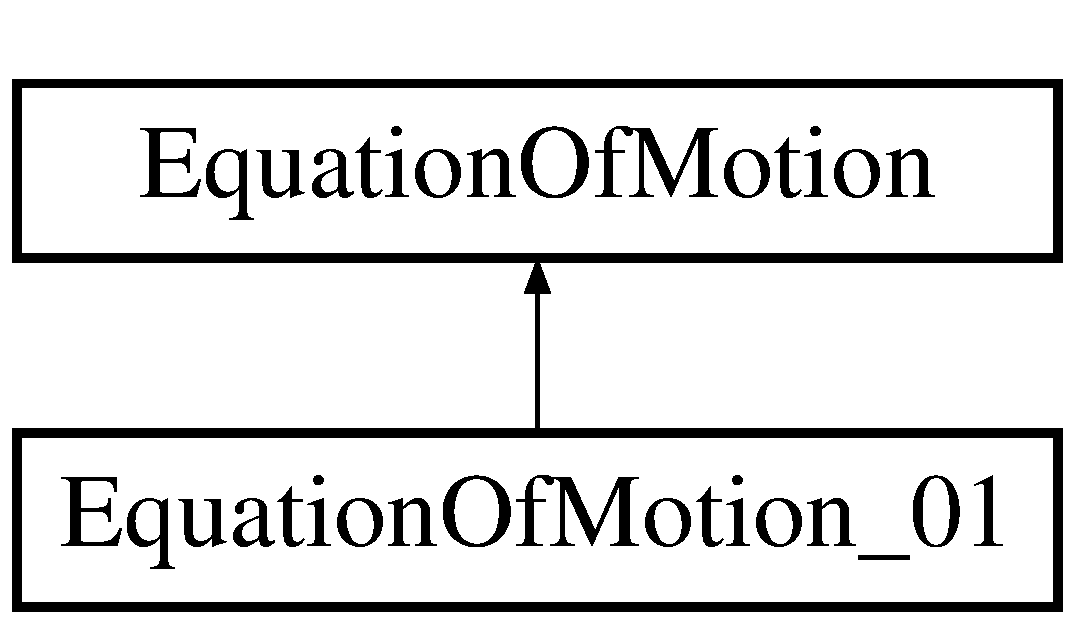
\includegraphics[height=2.000000cm]{class_equation_of_motion}
\end{center}
\end{figure}
\subsection*{Public Member Functions}
\begin{DoxyCompactItemize}
\item 
\hyperlink{class_equation_of_motion_abdb595c57202820b3c78518cb5d459e4}{Equation\-Of\-Motion} ()
\item 
\hyperlink{class_equation_of_motion_ac62caa9b6cdc62ff36d725637e53e62f}{$\sim$\-Equation\-Of\-Motion} ()
\item 
void \hyperlink{class_equation_of_motion_a2c1b3517a0f2aaef687c99fb6b4803dc}{set\-Wave\-Freq} (double)
\item 
virtual void \hyperlink{class_equation_of_motion_a340c67ae539fb20634e7b5bb8edf65f0}{set\-Body\-Data} (\hyperlink{class_body}{Body}, \hyperlink{class_user_forces}{User\-Forces})=0
\item 
\hyperlink{class_body_with_force_matrix}{Body\-With\-Force\-Matrix} \hyperlink{class_equation_of_motion_a7481a809cff3f63523885e1ac372fcc3}{get\-Body\-Force\-Data} ()
\item 
double \hyperlink{class_equation_of_motion_a2b16c339fe40262a4ef1f7b8b0036a01}{kronecker\-Delta} (int, int)
\item 
complex\-Double \hyperlink{class_equation_of_motion_a52e671f290c5a07d1187d56849c84060}{time\-Differentiation} (complex\-Double, int)
\end{DoxyCompactItemize}
\subsection*{Public Attributes}
\begin{DoxyCompactItemize}
\item 
\hyperlink{class_body_with_force_matrix}{Body\-With\-Force\-Matrix} \hyperlink{class_equation_of_motion_aef744ed7692bf6186bb976e0d53f972f}{new\-Body\-Matrix}
\end{DoxyCompactItemize}


\subsection{Detailed Description}
This abstract class holds for data for an equaion of motion. 

\subsection{Constructor \& Destructor Documentation}
\hypertarget{class_equation_of_motion_abdb595c57202820b3c78518cb5d459e4}{\index{Equation\-Of\-Motion@{Equation\-Of\-Motion}!Equation\-Of\-Motion@{Equation\-Of\-Motion}}
\index{Equation\-Of\-Motion@{Equation\-Of\-Motion}!EquationOfMotion@{Equation\-Of\-Motion}}
\subsubsection[{Equation\-Of\-Motion}]{\setlength{\rightskip}{0pt plus 5cm}Equation\-Of\-Motion\-::\-Equation\-Of\-Motion (
\begin{DoxyParamCaption}
{}
\end{DoxyParamCaption}
)}}\label{class_equation_of_motion_abdb595c57202820b3c78518cb5d459e4}
The default constructor. \hypertarget{class_equation_of_motion_ac62caa9b6cdc62ff36d725637e53e62f}{\index{Equation\-Of\-Motion@{Equation\-Of\-Motion}!$\sim$\-Equation\-Of\-Motion@{$\sim$\-Equation\-Of\-Motion}}
\index{$\sim$\-Equation\-Of\-Motion@{$\sim$\-Equation\-Of\-Motion}!EquationOfMotion@{Equation\-Of\-Motion}}
\subsubsection[{$\sim$\-Equation\-Of\-Motion}]{\setlength{\rightskip}{0pt plus 5cm}Equation\-Of\-Motion\-::$\sim$\-Equation\-Of\-Motion (
\begin{DoxyParamCaption}
{}
\end{DoxyParamCaption}
)}}\label{class_equation_of_motion_ac62caa9b6cdc62ff36d725637e53e62f}
The default destructor, nothing happens here. 

\subsection{Member Function Documentation}
\hypertarget{class_equation_of_motion_a7481a809cff3f63523885e1ac372fcc3}{\index{Equation\-Of\-Motion@{Equation\-Of\-Motion}!get\-Body\-Force\-Data@{get\-Body\-Force\-Data}}
\index{get\-Body\-Force\-Data@{get\-Body\-Force\-Data}!EquationOfMotion@{Equation\-Of\-Motion}}
\subsubsection[{get\-Body\-Force\-Data}]{\setlength{\rightskip}{0pt plus 5cm}{\bf Body\-With\-Force\-Matrix} Equation\-Of\-Motion\-::get\-Body\-Force\-Data (
\begin{DoxyParamCaption}
{}
\end{DoxyParamCaption}
)}}\label{class_equation_of_motion_a7481a809cff3f63523885e1ac372fcc3}
Retrieve the body with force matrix object. \begin{DoxyReturn}{Returns}
The body with force matrix object. 
\end{DoxyReturn}
\hypertarget{class_equation_of_motion_a2b16c339fe40262a4ef1f7b8b0036a01}{\index{Equation\-Of\-Motion@{Equation\-Of\-Motion}!kronecker\-Delta@{kronecker\-Delta}}
\index{kronecker\-Delta@{kronecker\-Delta}!EquationOfMotion@{Equation\-Of\-Motion}}
\subsubsection[{kronecker\-Delta}]{\setlength{\rightskip}{0pt plus 5cm}double Equation\-Of\-Motion\-::kronecker\-Delta (
\begin{DoxyParamCaption}
\item[{int}]{num1, }
\item[{int}]{num2}
\end{DoxyParamCaption}
)}}\label{class_equation_of_motion_a2b16c339fe40262a4ef1f7b8b0036a01}
Retrieve the body with force matrix object. 
\begin{DoxyParams}{Parameters}
{\em num1} & An int. \\
\hline
{\em num2} & An int. \\
\hline
\end{DoxyParams}
\begin{DoxyReturn}{Returns}
Return 0 if two numbers are equal or 1 if not. 
\end{DoxyReturn}
\hypertarget{class_equation_of_motion_a340c67ae539fb20634e7b5bb8edf65f0}{\index{Equation\-Of\-Motion@{Equation\-Of\-Motion}!set\-Body\-Data@{set\-Body\-Data}}
\index{set\-Body\-Data@{set\-Body\-Data}!EquationOfMotion@{Equation\-Of\-Motion}}
\subsubsection[{set\-Body\-Data}]{\setlength{\rightskip}{0pt plus 5cm}virtual void Equation\-Of\-Motion\-::set\-Body\-Data (
\begin{DoxyParamCaption}
\item[{{\bf Body}}]{, }
\item[{{\bf User\-Forces}}]{}
\end{DoxyParamCaption}
)\hspace{0.3cm}{\ttfamily [pure virtual]}}}\label{class_equation_of_motion_a340c67ae539fb20634e7b5bb8edf65f0}
This pure virtual function must be implemented by child classes. 
\begin{DoxyParams}{Parameters}
{\em The} & \hyperlink{class_body}{Body}. \\
\hline
{\em The} & User Forces. \\
\hline
\end{DoxyParams}


Implemented in \hyperlink{class_equation_of_motion__01_a97581ef832e495feda5c7f91a30bb8c8}{Equation\-Of\-Motion\-\_\-01}.

\hypertarget{class_equation_of_motion_a2c1b3517a0f2aaef687c99fb6b4803dc}{\index{Equation\-Of\-Motion@{Equation\-Of\-Motion}!set\-Wave\-Freq@{set\-Wave\-Freq}}
\index{set\-Wave\-Freq@{set\-Wave\-Freq}!EquationOfMotion@{Equation\-Of\-Motion}}
\subsubsection[{set\-Wave\-Freq}]{\setlength{\rightskip}{0pt plus 5cm}void Equation\-Of\-Motion\-::set\-Wave\-Freq (
\begin{DoxyParamCaption}
\item[{double}]{new\-Freq\-In}
\end{DoxyParamCaption}
)}}\label{class_equation_of_motion_a2c1b3517a0f2aaef687c99fb6b4803dc}
Sets the current wave frequency to be used. 
\begin{DoxyParams}{Parameters}
{\em new\-Freq\-In} & The current wave frequency. \\
\hline
\end{DoxyParams}
\hypertarget{class_equation_of_motion_a52e671f290c5a07d1187d56849c84060}{\index{Equation\-Of\-Motion@{Equation\-Of\-Motion}!time\-Differentiation@{time\-Differentiation}}
\index{time\-Differentiation@{time\-Differentiation}!EquationOfMotion@{Equation\-Of\-Motion}}
\subsubsection[{time\-Differentiation}]{\setlength{\rightskip}{0pt plus 5cm}complex\-Double Equation\-Of\-Motion\-::time\-Differentiation (
\begin{DoxyParamCaption}
\item[{complex\-Double}]{variable, }
\item[{int}]{order}
\end{DoxyParamCaption}
)}}\label{class_equation_of_motion_a52e671f290c5a07d1187d56849c84060}
Computes the time differention on the values passed in. 
\begin{DoxyParams}{Parameters}
{\em variable} & A force coefficient. \\
\hline
{\em order} & The order derivative. \\
\hline
\end{DoxyParams}
\begin{DoxyReturn}{Returns}
Returns the computed time differentiation. 
\end{DoxyReturn}


\subsection{Member Data Documentation}
\hypertarget{class_equation_of_motion_aef744ed7692bf6186bb976e0d53f972f}{\index{Equation\-Of\-Motion@{Equation\-Of\-Motion}!new\-Body\-Matrix@{new\-Body\-Matrix}}
\index{new\-Body\-Matrix@{new\-Body\-Matrix}!EquationOfMotion@{Equation\-Of\-Motion}}
\subsubsection[{new\-Body\-Matrix}]{\setlength{\rightskip}{0pt plus 5cm}{\bf Body\-With\-Force\-Matrix} Equation\-Of\-Motion\-::new\-Body\-Matrix}}\label{class_equation_of_motion_aef744ed7692bf6186bb976e0d53f972f}
The \hyperlink{class_body}{Body} with force matrix object.. 

The documentation for this class was generated from the following files\-:\begin{DoxyCompactItemize}
\item 
Visual Studio 2010/\-Projects/o\-Freq Windows V\-S2010/o\-Freq/equationofmotion.\-h\item 
Visual Studio 2010/\-Projects/o\-Freq Windows V\-S2010/o\-Freq/equationofmotion.\-cpp\end{DoxyCompactItemize}

\hypertarget{class_equation_of_motion__01}{\section{Equation\-Of\-Motion\-\_\-01 Class Reference}
\label{class_equation_of_motion__01}\index{Equation\-Of\-Motion\-\_\-01@{Equation\-Of\-Motion\-\_\-01}}
}


{\ttfamily \#include $<$equationofmotion\-\_\-01.\-h$>$}

Inheritance diagram for Equation\-Of\-Motion\-\_\-01\-:\begin{figure}[H]
\begin{center}
\leavevmode
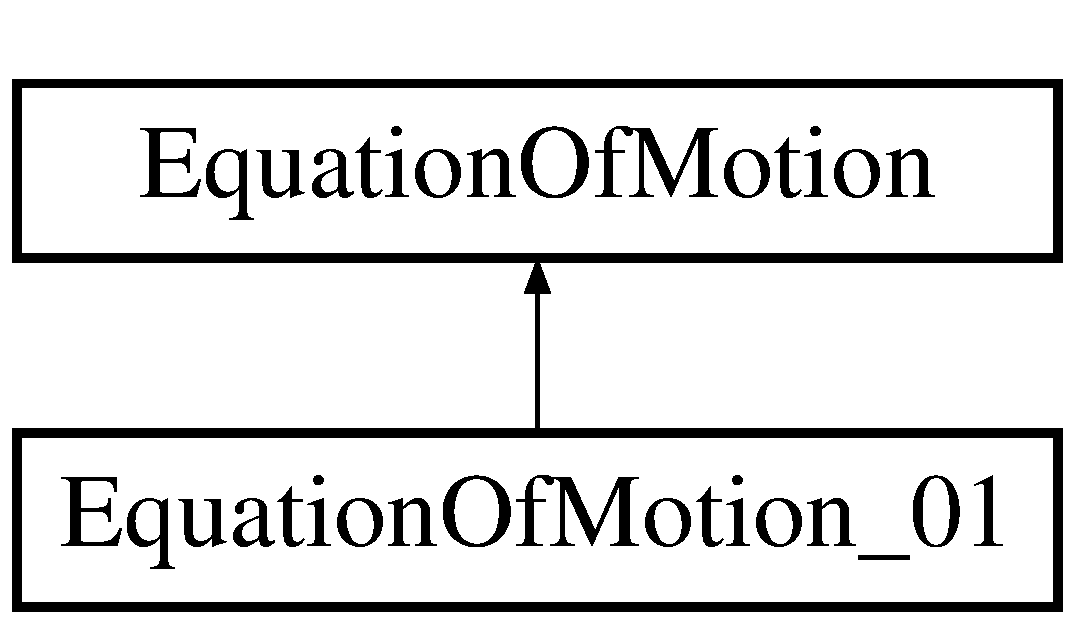
\includegraphics[height=2.000000cm]{class_equation_of_motion__01}
\end{center}
\end{figure}
\subsection*{Public Member Functions}
\begin{DoxyCompactItemize}
\item 
\hyperlink{class_equation_of_motion__01_aeb61f23820f4598eece331449e34643f}{Equation\-Of\-Motion\-\_\-01} ()
\item 
\hyperlink{class_equation_of_motion__01_ae771afba4d9d3b258008493413d0a3a2}{$\sim$\-Equation\-Of\-Motion\-\_\-01} ()
\item 
void \hyperlink{class_equation_of_motion__01_a97581ef832e495feda5c7f91a30bb8c8}{set\-Body\-Data} (\hyperlink{class_body}{Body}, \hyperlink{class_user_forces}{User\-Forces})
\item 
void \hyperlink{class_equation_of_motion__01_a5f38bbfdb6fde4267260216d49b01416}{calculate\-Equations} (\hyperlink{class_body_with_force_matrix}{Body\-With\-Force\-Matrix})
\item 
complex\-Double \hyperlink{class_equation_of_motion__01_a8d21abea0294b0631e5bcbb025a1912d}{get\-Body\-Mass\-Val} (int, int)
\item 
void \hyperlink{class_equation_of_motion__01_a2bd0fd9e562d494c9481f538f7661b1e}{set\-Body\-Mass\-Indexs} (int)
\item 
bool \hyperlink{class_equation_of_motion__01_a69f34f20a208c4b180e24a8aea815fd4}{is\-Current\-Body\-Mass\-Index} (int)
\end{DoxyCompactItemize}
\subsection*{Public Attributes}
\begin{DoxyCompactItemize}
\item 
int \hyperlink{class_equation_of_motion__01_a6f5e508b6824154b02267d7088ec6ba1}{body\-Mass\-Indexs} \mbox{[}body\-Equation\-Size\mbox{]}
\item 
cx\-\_\-mat \hyperlink{class_equation_of_motion__01_a735773656f31e5510aec14d72356801c}{solution\-Matrix}
\end{DoxyCompactItemize}


\subsection{Detailed Description}
This class holds data and functions to calculate the 6\-D\-O\-F \hyperlink{class_equation}{Equation} of Motion. 

\subsection{Constructor \& Destructor Documentation}
\hypertarget{class_equation_of_motion__01_aeb61f23820f4598eece331449e34643f}{\index{Equation\-Of\-Motion\-\_\-01@{Equation\-Of\-Motion\-\_\-01}!Equation\-Of\-Motion\-\_\-01@{Equation\-Of\-Motion\-\_\-01}}
\index{Equation\-Of\-Motion\-\_\-01@{Equation\-Of\-Motion\-\_\-01}!EquationOfMotion_01@{Equation\-Of\-Motion\-\_\-01}}
\subsubsection[{Equation\-Of\-Motion\-\_\-01}]{\setlength{\rightskip}{0pt plus 5cm}Equation\-Of\-Motion\-\_\-01\-::\-Equation\-Of\-Motion\-\_\-01 (
\begin{DoxyParamCaption}
{}
\end{DoxyParamCaption}
)}}\label{class_equation_of_motion__01_aeb61f23820f4598eece331449e34643f}
The default constructor. \hypertarget{class_equation_of_motion__01_ae771afba4d9d3b258008493413d0a3a2}{\index{Equation\-Of\-Motion\-\_\-01@{Equation\-Of\-Motion\-\_\-01}!$\sim$\-Equation\-Of\-Motion\-\_\-01@{$\sim$\-Equation\-Of\-Motion\-\_\-01}}
\index{$\sim$\-Equation\-Of\-Motion\-\_\-01@{$\sim$\-Equation\-Of\-Motion\-\_\-01}!EquationOfMotion_01@{Equation\-Of\-Motion\-\_\-01}}
\subsubsection[{$\sim$\-Equation\-Of\-Motion\-\_\-01}]{\setlength{\rightskip}{0pt plus 5cm}Equation\-Of\-Motion\-\_\-01\-::$\sim$\-Equation\-Of\-Motion\-\_\-01 (
\begin{DoxyParamCaption}
{}
\end{DoxyParamCaption}
)}}\label{class_equation_of_motion__01_ae771afba4d9d3b258008493413d0a3a2}
The default destructor, nothing happens here. 

\subsection{Member Function Documentation}
\hypertarget{class_equation_of_motion__01_a5f38bbfdb6fde4267260216d49b01416}{\index{Equation\-Of\-Motion\-\_\-01@{Equation\-Of\-Motion\-\_\-01}!calculate\-Equations@{calculate\-Equations}}
\index{calculate\-Equations@{calculate\-Equations}!EquationOfMotion_01@{Equation\-Of\-Motion\-\_\-01}}
\subsubsection[{calculate\-Equations}]{\setlength{\rightskip}{0pt plus 5cm}void Equation\-Of\-Motion\-\_\-01\-::calculate\-Equations (
\begin{DoxyParamCaption}
\item[{{\bf Body\-With\-Force\-Matrix}}]{the\-Body\-With\-Force\-Matrices}
\end{DoxyParamCaption}
)}}\label{class_equation_of_motion__01_a5f38bbfdb6fde4267260216d49b01416}
Perform the calculations for the 6\-D\-O\-F Motion Model. 
\begin{DoxyParams}{Parameters}
{\em the\-Body\-With\-Force\-Matrices} & The \hyperlink{class_body}{Body} with force matrices. \\
\hline
\end{DoxyParams}
\hypertarget{class_equation_of_motion__01_a8d21abea0294b0631e5bcbb025a1912d}{\index{Equation\-Of\-Motion\-\_\-01@{Equation\-Of\-Motion\-\_\-01}!get\-Body\-Mass\-Val@{get\-Body\-Mass\-Val}}
\index{get\-Body\-Mass\-Val@{get\-Body\-Mass\-Val}!EquationOfMotion_01@{Equation\-Of\-Motion\-\_\-01}}
\subsubsection[{get\-Body\-Mass\-Val}]{\setlength{\rightskip}{0pt plus 5cm}complex\-Double Equation\-Of\-Motion\-\_\-01\-::get\-Body\-Mass\-Val (
\begin{DoxyParamCaption}
\item[{int}]{equation\-Num, }
\item[{int}]{var}
\end{DoxyParamCaption}
)}}\label{class_equation_of_motion__01_a8d21abea0294b0631e5bcbb025a1912d}
Retrieve a variable in the equaion from the mass matrix. 
\begin{DoxyParams}{Parameters}
{\em equation\-Num} & The equation number (row in mass matrix). \\
\hline
{\em var} & The variable in the equation (column in mass matrix). \\
\hline
\end{DoxyParams}
\begin{DoxyReturn}{Returns}
The variable in the specified equation from the mass matrix. 
\end{DoxyReturn}
\hypertarget{class_equation_of_motion__01_a69f34f20a208c4b180e24a8aea815fd4}{\index{Equation\-Of\-Motion\-\_\-01@{Equation\-Of\-Motion\-\_\-01}!is\-Current\-Body\-Mass\-Index@{is\-Current\-Body\-Mass\-Index}}
\index{is\-Current\-Body\-Mass\-Index@{is\-Current\-Body\-Mass\-Index}!EquationOfMotion_01@{Equation\-Of\-Motion\-\_\-01}}
\subsubsection[{is\-Current\-Body\-Mass\-Index}]{\setlength{\rightskip}{0pt plus 5cm}bool Equation\-Of\-Motion\-\_\-01\-::is\-Current\-Body\-Mass\-Index (
\begin{DoxyParamCaption}
\item[{int}]{cur\-Index}
\end{DoxyParamCaption}
)}}\label{class_equation_of_motion__01_a69f34f20a208c4b180e24a8aea815fd4}
Check if current index is valid in the mass matrix. 
\begin{DoxyParams}{Parameters}
{\em cur\-Index} & The current index in mass matrix. return True if a valid entry in mass matrix. \\
\hline
\end{DoxyParams}
\hypertarget{class_equation_of_motion__01_a97581ef832e495feda5c7f91a30bb8c8}{\index{Equation\-Of\-Motion\-\_\-01@{Equation\-Of\-Motion\-\_\-01}!set\-Body\-Data@{set\-Body\-Data}}
\index{set\-Body\-Data@{set\-Body\-Data}!EquationOfMotion_01@{Equation\-Of\-Motion\-\_\-01}}
\subsubsection[{set\-Body\-Data}]{\setlength{\rightskip}{0pt plus 5cm}void Equation\-Of\-Motion\-\_\-01\-::set\-Body\-Data (
\begin{DoxyParamCaption}
\item[{{\bf Body}}]{body\-Data\-In, }
\item[{{\bf User\-Forces}}]{user\-Forces\-In}
\end{DoxyParamCaption}
)\hspace{0.3cm}{\ttfamily [virtual]}}}\label{class_equation_of_motion__01_a97581ef832e495feda5c7f91a30bb8c8}
Sets the body and forces data for this object. 
\begin{DoxyParams}{Parameters}
{\em body\-Data\-In} & The \hyperlink{class_body}{Body}. \\
\hline
{\em user\-Forces\-In} & The user forces. \\
\hline
\end{DoxyParams}


Implements \hyperlink{class_equation_of_motion_a340c67ae539fb20634e7b5bb8edf65f0}{Equation\-Of\-Motion}.

\hypertarget{class_equation_of_motion__01_a2bd0fd9e562d494c9481f538f7661b1e}{\index{Equation\-Of\-Motion\-\_\-01@{Equation\-Of\-Motion\-\_\-01}!set\-Body\-Mass\-Indexs@{set\-Body\-Mass\-Indexs}}
\index{set\-Body\-Mass\-Indexs@{set\-Body\-Mass\-Indexs}!EquationOfMotion_01@{Equation\-Of\-Motion\-\_\-01}}
\subsubsection[{set\-Body\-Mass\-Indexs}]{\setlength{\rightskip}{0pt plus 5cm}void Equation\-Of\-Motion\-\_\-01\-::set\-Body\-Mass\-Indexs (
\begin{DoxyParamCaption}
\item[{int}]{cur\-Index}
\end{DoxyParamCaption}
)}}\label{class_equation_of_motion__01_a2bd0fd9e562d494c9481f538f7661b1e}
Sets the Indexs in solution matrix, This Needs to be fixed, only supports 2 bodies max. 
\begin{DoxyParams}{Parameters}
{\em cur\-Index} & The current index in the matrix. \\
\hline
\end{DoxyParams}


\subsection{Member Data Documentation}
\hypertarget{class_equation_of_motion__01_a6f5e508b6824154b02267d7088ec6ba1}{\index{Equation\-Of\-Motion\-\_\-01@{Equation\-Of\-Motion\-\_\-01}!body\-Mass\-Indexs@{body\-Mass\-Indexs}}
\index{body\-Mass\-Indexs@{body\-Mass\-Indexs}!EquationOfMotion_01@{Equation\-Of\-Motion\-\_\-01}}
\subsubsection[{body\-Mass\-Indexs}]{\setlength{\rightskip}{0pt plus 5cm}int Equation\-Of\-Motion\-\_\-01\-::body\-Mass\-Indexs\mbox{[}body\-Equation\-Size\mbox{]}}}\label{class_equation_of_motion__01_a6f5e508b6824154b02267d7088ec6ba1}
The indexs in solution matrix for all sub matrices. \hypertarget{class_equation_of_motion__01_a735773656f31e5510aec14d72356801c}{\index{Equation\-Of\-Motion\-\_\-01@{Equation\-Of\-Motion\-\_\-01}!solution\-Matrix@{solution\-Matrix}}
\index{solution\-Matrix@{solution\-Matrix}!EquationOfMotion_01@{Equation\-Of\-Motion\-\_\-01}}
\subsubsection[{solution\-Matrix}]{\setlength{\rightskip}{0pt plus 5cm}cx\-\_\-mat Equation\-Of\-Motion\-\_\-01\-::solution\-Matrix}}\label{class_equation_of_motion__01_a735773656f31e5510aec14d72356801c}
The solution matirx. 

The documentation for this class was generated from the following files\-:\begin{DoxyCompactItemize}
\item 
Visual Studio 2010/\-Projects/o\-Freq Windows V\-S2010/o\-Freq/equationofmotion\-\_\-01.\-h\item 
Visual Studio 2010/\-Projects/o\-Freq Windows V\-S2010/o\-Freq/equationofmotion\-\_\-01.\-cpp\end{DoxyCompactItemize}

\hypertarget{class_file_writer}{\section{File\-Writer Class Reference}
\label{class_file_writer}\index{File\-Writer@{File\-Writer}}
}


{\ttfamily \#include $<$filewriter.\-h$>$}

\subsection*{Public Member Functions}
\begin{DoxyCompactItemize}
\item 
\hypertarget{class_file_writer_aa6b362f5b306dd3409af81a463e97f40}{\hyperlink{class_file_writer_aa6b362f5b306dd3409af81a463e97f40}{File\-Writer} ()}\label{class_file_writer_aa6b362f5b306dd3409af81a463e97f40}

\begin{DoxyCompactList}\small\item\em The default constructor. \end{DoxyCompactList}\item 
\hyperlink{class_file_writer_a08b98dceafbf0cd0875197072dfd7d58}{File\-Writer} (string root\-Path, \hyperlink{class_outputs_body}{Outputs\-Body} \&Body\-In)
\begin{DoxyCompactList}\small\item\em Constructor that includes the two important properties that must be declared for \hyperlink{class_file_writer}{File\-Writer} to work correctly. The root path for the project must be declared. And the pointer to the \hyperlink{class_outputs_body}{Outputs\-Body} object must be declared. \end{DoxyCompactList}\item 
\hyperlink{class_file_writer_ae5490307dcaf9237f4c1b8b8df433e03}{$\sim$\-File\-Writer} ()
\item 
void \hyperlink{class_file_writer_a15370335402192f7e5342a6049f664fc}{set\-Project\-Dir} (string dir\-In)
\begin{DoxyCompactList}\small\item\em Sets the path to the project directory. Assumes the string specifying the path does not end with a slash mark. The class will automatically add the slash mark. If a slash mark is present, the function will automatically remove it. \end{DoxyCompactList}\item 
bool \hyperlink{class_file_writer_a74a40c3c47b4d12582a2aa44c38d9d07}{clear\-Files} ()
\item 
\hyperlink{class_outputs_body}{Outputs\-Body} \& \hyperlink{class_file_writer_a77da1b41e1332209f39243fcca4d1287}{ref\-Outputs\-Body} ()
\begin{DoxyCompactList}\small\item\em Provides direct access to the \hyperlink{class_outputs_body}{Outputs\-Body} object. The \hyperlink{class_outputs_body}{Outputs\-Body} object must be set for the file\-Writer to work. All file data comes from the \hyperlink{class_file_writer}{File\-Writer} object. \end{DoxyCompactList}\item 
bool \hyperlink{class_file_writer_a268a7349181f2d8c739a0809ba0eede2}{file\-Exists} (string filename)
\begin{DoxyCompactList}\small\item\em Test is a file exists. Function automatically assumes that the file is located in the directory associated with the \hyperlink{class_file_writer_a9748d987475a225b49e14f48b8be0cd6}{get\-Cur\-Wave\-Ind()} function. Returns true if the file exists and is valid. Returns false if the file does not exist or the directory does not exist. \end{DoxyCompactList}\item 
bool \hyperlink{class_file_writer_a0428a4f8ad72d01ff5316bfa3e4ce631}{write\-Wave\-Direction} ()
\begin{DoxyCompactList}\small\item\em Writes the directions list to file. \end{DoxyCompactList}\item 
bool \hyperlink{class_file_writer_ac6df31af71020a41adb6ecd6ff136532}{write\-Frequency} ()
\item 
bool \hyperlink{class_file_writer_a5c921b5ae92039cf50458e2c46e204da}{write\-Global\-Motion} ()
\begin{DoxyCompactList}\small\item\em Writes the output file of global motions. If file exists, appends to the file, assuming the appended file is a new body object. \end{DoxyCompactList}\item 
bool \hyperlink{class_file_writer_a2078a50dbd21946aeed86d8e0bccd50e}{write\-Global\-Velocity} ()
\begin{DoxyCompactList}\small\item\em Writes the output file of global velocities. If file exists, appends to the file, assuming the appended file is a new body object. \end{DoxyCompactList}\item 
bool \hyperlink{class_file_writer_aaff553c2e03cb1c1639e107cfeac3038}{write\-Global\-Acceleration} ()
\begin{DoxyCompactList}\small\item\em Writes the output file of global accelerations. If file exists, appends to the file, assuming the appended file is a new body object. \end{DoxyCompactList}\item 
bool \hyperlink{class_file_writer_a317649499b8c16dd529e2bf588e3be88}{write\-Global\-Solution} ()
\begin{DoxyCompactList}\small\item\em Writes the output file of global solutions. If file exists, appends to the file, assuming the appended file is a new body object. \end{DoxyCompactList}\end{DoxyCompactItemize}
\subsection*{Protected Member Functions}
\begin{DoxyCompactItemize}
\item 
int \hyperlink{class_file_writer_a9748d987475a225b49e14f48b8be0cd6}{get\-Cur\-Wave\-Ind} ()
\begin{DoxyCompactList}\small\item\em Gets the index of the current wave direction. The index is used to specify which directory to write the file into. \end{DoxyCompactList}\item 
string \hyperlink{class_file_writer_a82a3acb66bd5c0396836386258608a40}{get\-Cur\-Wave\-Dir} ()
\begin{DoxyCompactList}\small\item\em Returns the string containing the folder path for the current wave direction. Path name includes the slash mark. For example, if using wave index 0, the string output would be\-: \char`\"{}d0/\char`\"{}. \end{DoxyCompactList}\item 
bool \hyperlink{class_file_writer_ae6e5afc50484694d033628c954c62df3}{create\-Dir} (string path)
\begin{DoxyCompactList}\small\item\em Creates the directory specified by the string path. Assumes any specified directory is under the root project directory. \end{DoxyCompactList}\item 
\hypertarget{class_file_writer_aeea3ca877f0c5280b22ea7ff653db233}{void \hyperlink{class_file_writer_aeea3ca877f0c5280b22ea7ff653db233}{set\-Header} ()}\label{class_file_writer_aeea3ca877f0c5280b22ea7ff653db233}

\begin{DoxyCompactList}\small\item\em Reads in from input file the header to be used in all files. This is a basic header text that should be at the top of all Open\-S\-E\-A output files. Simple identification of the program. Nothing specific for output. \end{DoxyCompactList}\item 
string \hyperlink{class_file_writer_a419b9ba153151766c7a8c68717a11778}{get\-Info\-Block} (string name\-In)
\end{DoxyCompactItemize}


\subsection{Detailed Description}
This class write all outputs to files. All output data is based on the attached \hyperlink{class_outputs_body}{Outputs\-Body} object. To use the filewriter object, follow this sequence of steps\-: 1.) Create object. 2.) Set \hyperlink{class_outputs_body}{Outputs\-Body} object associated with the file. 3.) Set the filesystem path to the root directory for the current run of ofreq. 4.) Run the \hyperlink{class_file_writer_a74a40c3c47b4d12582a2aa44c38d9d07}{clear\-Files()} function, which will clear out any pre-\/existing files. 5.) Run the write\-File function for the specified file that you want to write out.

Note that the \hyperlink{class_outputs_body}{Outputs\-Body} object also provides the information on the current wave direction. And the \hyperlink{class_file_writer}{File\-Writer} changes its directory to write to depending on the current wave direction. So the \hyperlink{class_outputs_body}{Outputs\-Body} object must be updated before writing a new wave direction. 

\subsection{Constructor \& Destructor Documentation}
\hypertarget{class_file_writer_a08b98dceafbf0cd0875197072dfd7d58}{\index{File\-Writer@{File\-Writer}!File\-Writer@{File\-Writer}}
\index{File\-Writer@{File\-Writer}!FileWriter@{File\-Writer}}
\subsubsection[{File\-Writer}]{\setlength{\rightskip}{0pt plus 5cm}File\-Writer\-::\-File\-Writer (
\begin{DoxyParamCaption}
\item[{string}]{root\-Path, }
\item[{{\bf Outputs\-Body} \&}]{Body\-In}
\end{DoxyParamCaption}
)}}\label{class_file_writer_a08b98dceafbf0cd0875197072dfd7d58}


Constructor that includes the two important properties that must be declared for \hyperlink{class_file_writer}{File\-Writer} to work correctly. The root path for the project must be declared. And the pointer to the \hyperlink{class_outputs_body}{Outputs\-Body} object must be declared. 


\begin{DoxyParams}{Parameters}
{\em root\-Path} & The full fule system path to the root directory of the currently running o\-Freq project. Not the path to the o\-Freq executable files. This is the path to the directory containing input and output files. \\
\hline
{\em Body\-In} & The \hyperlink{class_outputs_body}{Outputs\-Body} object that will be used to write out data for the \hyperlink{class_file_writer}{File\-Writer}. The \hyperlink{class_outputs_body}{Outputs\-Body} object supplies the data, and the \hyperlink{class_file_writer}{File\-Writer} writes that data to the A\-S\-C\-I\-I text file. The \hyperlink{class_outputs_body}{Outputs\-Body} object also provides the information on the current wave direction. So the \hyperlink{class_outputs_body}{Outputs\-Body} object must be updated before writing a new wave direction. \\
\hline
\end{DoxyParams}
\begin{DoxySeeAlso}{See Also}
\hyperlink{class_outputs_body}{Outputs\-Body} 
\end{DoxySeeAlso}


Here is the call graph for this function\-:\nopagebreak
\begin{figure}[H]
\begin{center}
\leavevmode
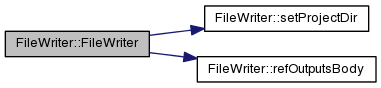
\includegraphics[width=350pt]{class_file_writer_a08b98dceafbf0cd0875197072dfd7d58_cgraph}
\end{center}
\end{figure}


\hypertarget{class_file_writer_ae5490307dcaf9237f4c1b8b8df433e03}{\index{File\-Writer@{File\-Writer}!$\sim$\-File\-Writer@{$\sim$\-File\-Writer}}
\index{$\sim$\-File\-Writer@{$\sim$\-File\-Writer}!FileWriter@{File\-Writer}}
\subsubsection[{$\sim$\-File\-Writer}]{\setlength{\rightskip}{0pt plus 5cm}File\-Writer\-::$\sim$\-File\-Writer (
\begin{DoxyParamCaption}
{}
\end{DoxyParamCaption}
)}}\label{class_file_writer_ae5490307dcaf9237f4c1b8b8df433e03}
The default destructor, nothing happens here. 

\subsection{Member Function Documentation}
\hypertarget{class_file_writer_a74a40c3c47b4d12582a2aa44c38d9d07}{\index{File\-Writer@{File\-Writer}!clear\-Files@{clear\-Files}}
\index{clear\-Files@{clear\-Files}!FileWriter@{File\-Writer}}
\subsubsection[{clear\-Files}]{\setlength{\rightskip}{0pt plus 5cm}bool File\-Writer\-::clear\-Files (
\begin{DoxyParamCaption}
{}
\end{DoxyParamCaption}
)}}\label{class_file_writer_a74a40c3c47b4d12582a2aa44c38d9d07}
Remove all old directiories \& files written by o\-Freq previous run. \begin{DoxyReturn}{Returns}
Return true if all files \& directories were successfully deleted. 
\end{DoxyReturn}
\hypertarget{class_file_writer_ae6e5afc50484694d033628c954c62df3}{\index{File\-Writer@{File\-Writer}!create\-Dir@{create\-Dir}}
\index{create\-Dir@{create\-Dir}!FileWriter@{File\-Writer}}
\subsubsection[{create\-Dir}]{\setlength{\rightskip}{0pt plus 5cm}bool File\-Writer\-::create\-Dir (
\begin{DoxyParamCaption}
\item[{string}]{path}
\end{DoxyParamCaption}
)\hspace{0.3cm}{\ttfamily [protected]}}}\label{class_file_writer_ae6e5afc50484694d033628c954c62df3}


Creates the directory specified by the string path. Assumes any specified directory is under the root project directory. 


\begin{DoxyParams}{Parameters}
{\em path} & String. The path of the directory to create. \\
\hline
\end{DoxyParams}
\begin{DoxyReturn}{Returns}
Returns true if creation sucessful. 
\end{DoxyReturn}


Here is the caller graph for this function\-:\nopagebreak
\begin{figure}[H]
\begin{center}
\leavevmode
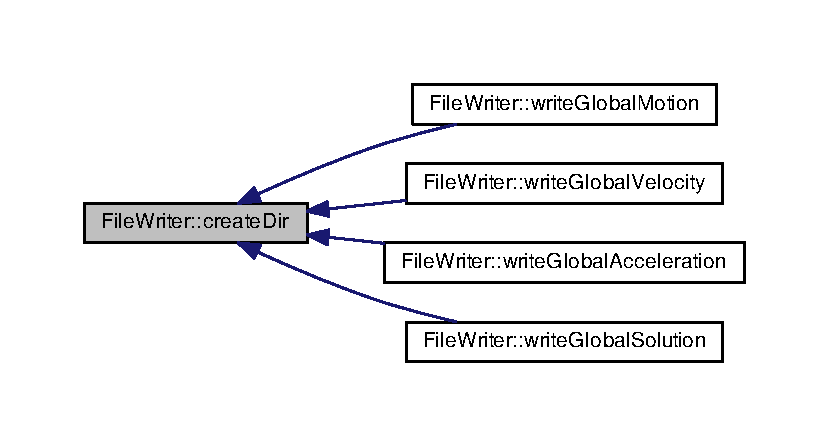
\includegraphics[width=350pt]{class_file_writer_ae6e5afc50484694d033628c954c62df3_icgraph}
\end{center}
\end{figure}


\hypertarget{class_file_writer_a268a7349181f2d8c739a0809ba0eede2}{\index{File\-Writer@{File\-Writer}!file\-Exists@{file\-Exists}}
\index{file\-Exists@{file\-Exists}!FileWriter@{File\-Writer}}
\subsubsection[{file\-Exists}]{\setlength{\rightskip}{0pt plus 5cm}bool File\-Writer\-::file\-Exists (
\begin{DoxyParamCaption}
\item[{string}]{filename}
\end{DoxyParamCaption}
)}}\label{class_file_writer_a268a7349181f2d8c739a0809ba0eede2}


Test is a file exists. Function automatically assumes that the file is located in the directory associated with the \hyperlink{class_file_writer_a9748d987475a225b49e14f48b8be0cd6}{get\-Cur\-Wave\-Ind()} function. Returns true if the file exists and is valid. Returns false if the file does not exist or the directory does not exist. 


\begin{DoxyParams}{Parameters}
{\em filename} & String. Specifies the filename to search for. Only needs to specify local filename. Directory information is already inferred from previous settings with the \hyperlink{class_outputs_body}{Outputs\-Body} object. \\
\hline
\end{DoxyParams}
\begin{DoxyReturn}{Returns}
Returns boolean variable. True if the file exists. False if the file or any required directories do not exist. 
\end{DoxyReturn}
\begin{DoxySeeAlso}{See Also}
\hyperlink{class_file_writer_a9748d987475a225b49e14f48b8be0cd6}{File\-Writer\-::get\-Cur\-Wave\-Ind()} 
\end{DoxySeeAlso}


Here is the call graph for this function\-:\nopagebreak
\begin{figure}[H]
\begin{center}
\leavevmode
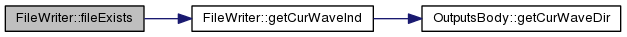
\includegraphics[width=350pt]{class_file_writer_a268a7349181f2d8c739a0809ba0eede2_cgraph}
\end{center}
\end{figure}


\hypertarget{class_file_writer_a82a3acb66bd5c0396836386258608a40}{\index{File\-Writer@{File\-Writer}!get\-Cur\-Wave\-Dir@{get\-Cur\-Wave\-Dir}}
\index{get\-Cur\-Wave\-Dir@{get\-Cur\-Wave\-Dir}!FileWriter@{File\-Writer}}
\subsubsection[{get\-Cur\-Wave\-Dir}]{\setlength{\rightskip}{0pt plus 5cm}string File\-Writer\-::get\-Cur\-Wave\-Dir (
\begin{DoxyParamCaption}
{}
\end{DoxyParamCaption}
)\hspace{0.3cm}{\ttfamily [protected]}}}\label{class_file_writer_a82a3acb66bd5c0396836386258608a40}


Returns the string containing the folder path for the current wave direction. Path name includes the slash mark. For example, if using wave index 0, the string output would be\-: \char`\"{}d0/\char`\"{}. 

\begin{DoxyReturn}{Returns}
String output. Has the path name for the current wave directory. 
\end{DoxyReturn}


Here is the call graph for this function\-:\nopagebreak
\begin{figure}[H]
\begin{center}
\leavevmode
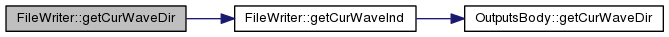
\includegraphics[width=350pt]{class_file_writer_a82a3acb66bd5c0396836386258608a40_cgraph}
\end{center}
\end{figure}




Here is the caller graph for this function\-:\nopagebreak
\begin{figure}[H]
\begin{center}
\leavevmode
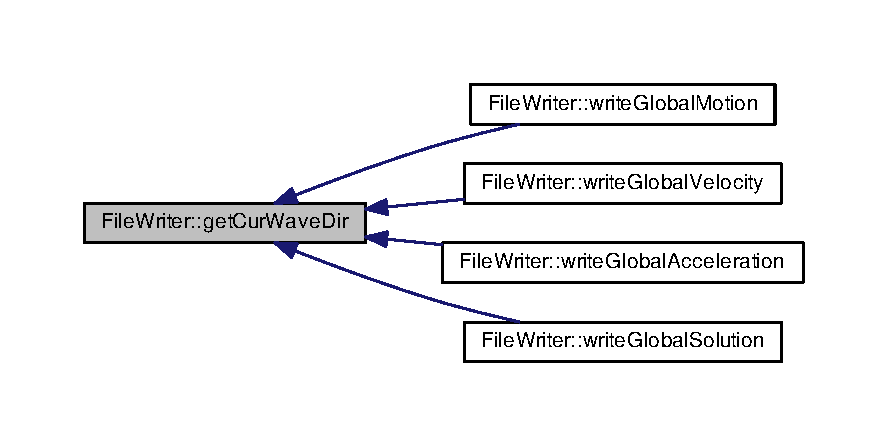
\includegraphics[width=350pt]{class_file_writer_a82a3acb66bd5c0396836386258608a40_icgraph}
\end{center}
\end{figure}


\hypertarget{class_file_writer_a9748d987475a225b49e14f48b8be0cd6}{\index{File\-Writer@{File\-Writer}!get\-Cur\-Wave\-Ind@{get\-Cur\-Wave\-Ind}}
\index{get\-Cur\-Wave\-Ind@{get\-Cur\-Wave\-Ind}!FileWriter@{File\-Writer}}
\subsubsection[{get\-Cur\-Wave\-Ind}]{\setlength{\rightskip}{0pt plus 5cm}int File\-Writer\-::get\-Cur\-Wave\-Ind (
\begin{DoxyParamCaption}
{}
\end{DoxyParamCaption}
)\hspace{0.3cm}{\ttfamily [protected]}}}\label{class_file_writer_a9748d987475a225b49e14f48b8be0cd6}


Gets the index of the current wave direction. The index is used to specify which directory to write the file into. 

\begin{DoxyReturn}{Returns}
Returns integer which specifies the index of the current wave direction. Index specifies the wave direction in the list of wave directions. Valid values are any integer from 0 or greater. 
\end{DoxyReturn}


Here is the call graph for this function\-:\nopagebreak
\begin{figure}[H]
\begin{center}
\leavevmode
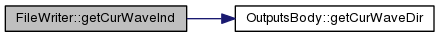
\includegraphics[width=350pt]{class_file_writer_a9748d987475a225b49e14f48b8be0cd6_cgraph}
\end{center}
\end{figure}




Here is the caller graph for this function\-:\nopagebreak
\begin{figure}[H]
\begin{center}
\leavevmode
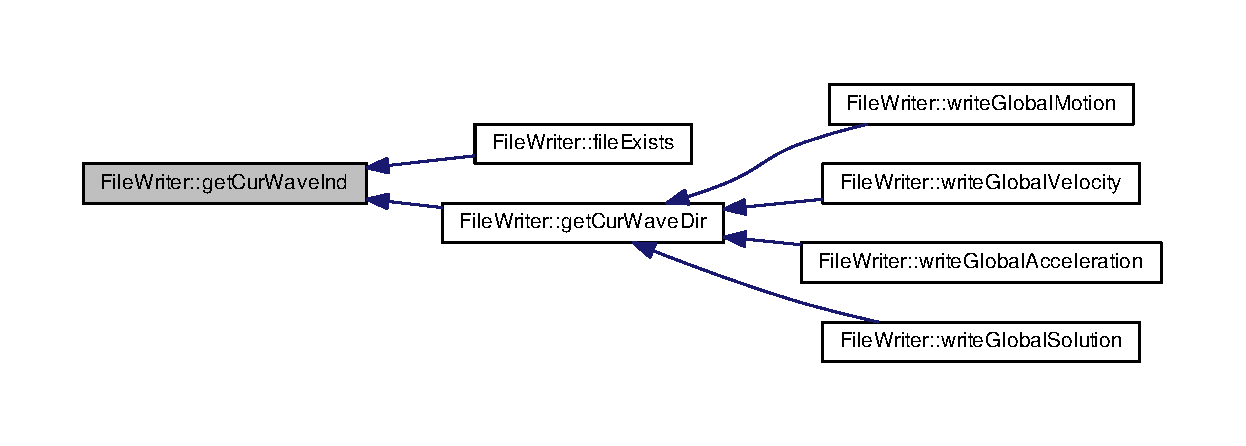
\includegraphics[width=350pt]{class_file_writer_a9748d987475a225b49e14f48b8be0cd6_icgraph}
\end{center}
\end{figure}


\hypertarget{class_file_writer_a419b9ba153151766c7a8c68717a11778}{\index{File\-Writer@{File\-Writer}!get\-Info\-Block@{get\-Info\-Block}}
\index{get\-Info\-Block@{get\-Info\-Block}!FileWriter@{File\-Writer}}
\subsubsection[{get\-Info\-Block}]{\setlength{\rightskip}{0pt plus 5cm}string File\-Writer\-::get\-Info\-Block (
\begin{DoxyParamCaption}
\item[{string}]{name\-In}
\end{DoxyParamCaption}
)\hspace{0.3cm}{\ttfamily [protected]}}}\label{class_file_writer_a419b9ba153151766c7a8c68717a11778}
Set information about the file to be written after header and above data, included in the seafile block. 
\begin{DoxyParams}{Parameters}
{\em name\-In} & The name of the object. \\
\hline
\end{DoxyParams}
\begin{DoxyReturn}{Returns}
Returns string. String contains the file info for the output file. Everything written into the seafile block. Variable passed by value. 
\end{DoxyReturn}


Here is the caller graph for this function\-:\nopagebreak
\begin{figure}[H]
\begin{center}
\leavevmode
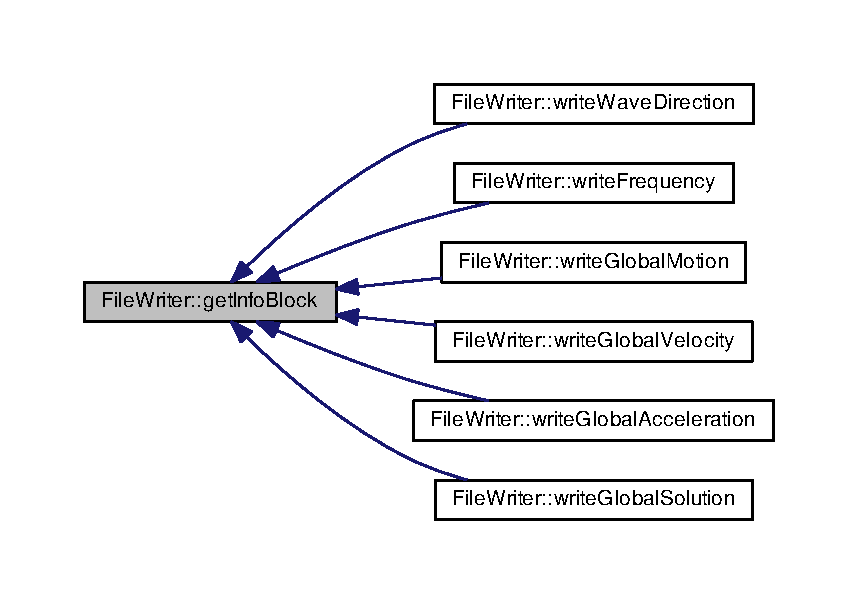
\includegraphics[width=350pt]{class_file_writer_a419b9ba153151766c7a8c68717a11778_icgraph}
\end{center}
\end{figure}


\hypertarget{class_file_writer_a77da1b41e1332209f39243fcca4d1287}{\index{File\-Writer@{File\-Writer}!ref\-Outputs\-Body@{ref\-Outputs\-Body}}
\index{ref\-Outputs\-Body@{ref\-Outputs\-Body}!FileWriter@{File\-Writer}}
\subsubsection[{ref\-Outputs\-Body}]{\setlength{\rightskip}{0pt plus 5cm}{\bf Outputs\-Body} \& File\-Writer\-::ref\-Outputs\-Body (
\begin{DoxyParamCaption}
{}
\end{DoxyParamCaption}
)}}\label{class_file_writer_a77da1b41e1332209f39243fcca4d1287}


Provides direct access to the \hyperlink{class_outputs_body}{Outputs\-Body} object. The \hyperlink{class_outputs_body}{Outputs\-Body} object must be set for the file\-Writer to work. All file data comes from the \hyperlink{class_file_writer}{File\-Writer} object. 

\begin{DoxyReturn}{Returns}
Returns pointer to the \hyperlink{class_outputs_body}{Outputs\-Body} object. Variable passed by reference. 
\end{DoxyReturn}


Here is the caller graph for this function\-:\nopagebreak
\begin{figure}[H]
\begin{center}
\leavevmode
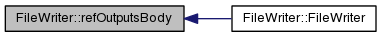
\includegraphics[width=350pt]{class_file_writer_a77da1b41e1332209f39243fcca4d1287_icgraph}
\end{center}
\end{figure}


\hypertarget{class_file_writer_a15370335402192f7e5342a6049f664fc}{\index{File\-Writer@{File\-Writer}!set\-Project\-Dir@{set\-Project\-Dir}}
\index{set\-Project\-Dir@{set\-Project\-Dir}!FileWriter@{File\-Writer}}
\subsubsection[{set\-Project\-Dir}]{\setlength{\rightskip}{0pt plus 5cm}void File\-Writer\-::set\-Project\-Dir (
\begin{DoxyParamCaption}
\item[{string}]{dir\-In}
\end{DoxyParamCaption}
)}}\label{class_file_writer_a15370335402192f7e5342a6049f664fc}


Sets the path to the project directory. Assumes the string specifying the path does not end with a slash mark. The class will automatically add the slash mark. If a slash mark is present, the function will automatically remove it. 


\begin{DoxyParams}{Parameters}
{\em dir\-In} & String specifying the path to the project directory. Variable passed by value. \\
\hline
\end{DoxyParams}


Here is the caller graph for this function\-:\nopagebreak
\begin{figure}[H]
\begin{center}
\leavevmode
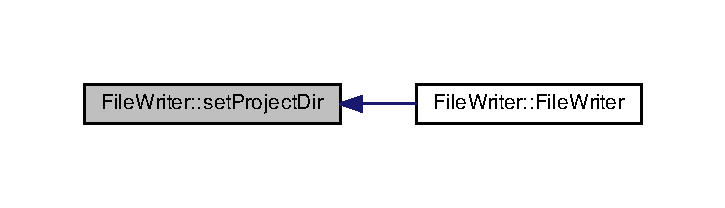
\includegraphics[width=348pt]{class_file_writer_a15370335402192f7e5342a6049f664fc_icgraph}
\end{center}
\end{figure}


\hypertarget{class_file_writer_ac6df31af71020a41adb6ecd6ff136532}{\index{File\-Writer@{File\-Writer}!write\-Frequency@{write\-Frequency}}
\index{write\-Frequency@{write\-Frequency}!FileWriter@{File\-Writer}}
\subsubsection[{write\-Frequency}]{\setlength{\rightskip}{0pt plus 5cm}bool File\-Writer\-::write\-Frequency (
\begin{DoxyParamCaption}
{}
\end{DoxyParamCaption}
)}}\label{class_file_writer_ac6df31af71020a41adb6ecd6ff136532}
Writes the frequencies list to file. \begin{DoxyReturn}{Returns}
true if write successful. 
\end{DoxyReturn}


Here is the call graph for this function\-:\nopagebreak
\begin{figure}[H]
\begin{center}
\leavevmode
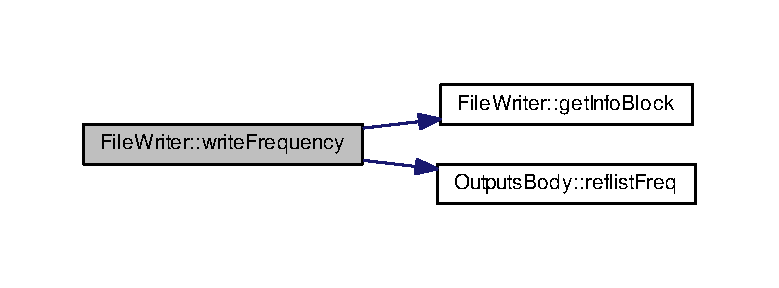
\includegraphics[width=350pt]{class_file_writer_ac6df31af71020a41adb6ecd6ff136532_cgraph}
\end{center}
\end{figure}


\hypertarget{class_file_writer_aaff553c2e03cb1c1639e107cfeac3038}{\index{File\-Writer@{File\-Writer}!write\-Global\-Acceleration@{write\-Global\-Acceleration}}
\index{write\-Global\-Acceleration@{write\-Global\-Acceleration}!FileWriter@{File\-Writer}}
\subsubsection[{write\-Global\-Acceleration}]{\setlength{\rightskip}{0pt plus 5cm}bool File\-Writer\-::write\-Global\-Acceleration (
\begin{DoxyParamCaption}
{}
\end{DoxyParamCaption}
)}}\label{class_file_writer_aaff553c2e03cb1c1639e107cfeac3038}


Writes the output file of global accelerations. If file exists, appends to the file, assuming the appended file is a new body object. 

\begin{DoxyReturn}{Returns}
Returns true if write successful. 
\end{DoxyReturn}


Here is the call graph for this function\-:\nopagebreak
\begin{figure}[H]
\begin{center}
\leavevmode
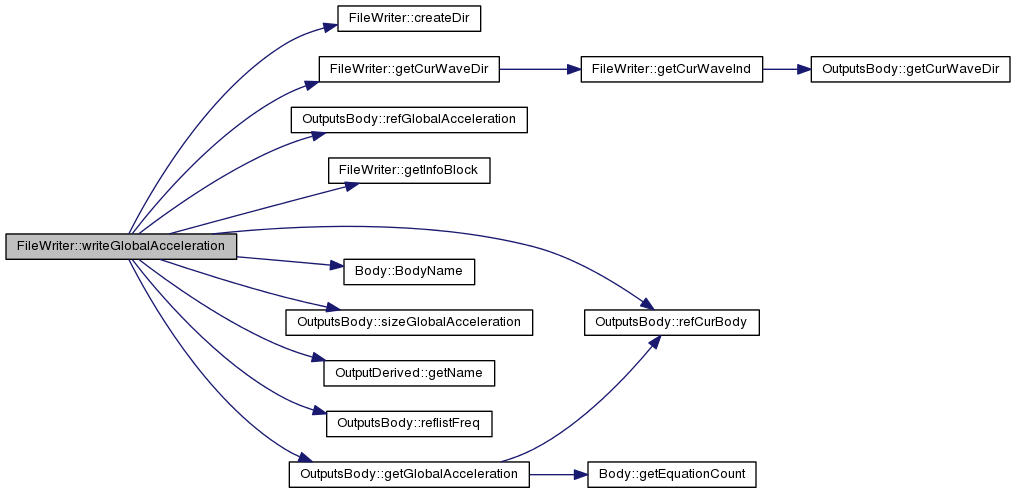
\includegraphics[width=350pt]{class_file_writer_aaff553c2e03cb1c1639e107cfeac3038_cgraph}
\end{center}
\end{figure}


\hypertarget{class_file_writer_a5c921b5ae92039cf50458e2c46e204da}{\index{File\-Writer@{File\-Writer}!write\-Global\-Motion@{write\-Global\-Motion}}
\index{write\-Global\-Motion@{write\-Global\-Motion}!FileWriter@{File\-Writer}}
\subsubsection[{write\-Global\-Motion}]{\setlength{\rightskip}{0pt plus 5cm}bool File\-Writer\-::write\-Global\-Motion (
\begin{DoxyParamCaption}
{}
\end{DoxyParamCaption}
)}}\label{class_file_writer_a5c921b5ae92039cf50458e2c46e204da}


Writes the output file of global motions. If file exists, appends to the file, assuming the appended file is a new body object. 

\begin{DoxyReturn}{Returns}
Returns true if write successful. 
\end{DoxyReturn}


Here is the call graph for this function\-:\nopagebreak
\begin{figure}[H]
\begin{center}
\leavevmode
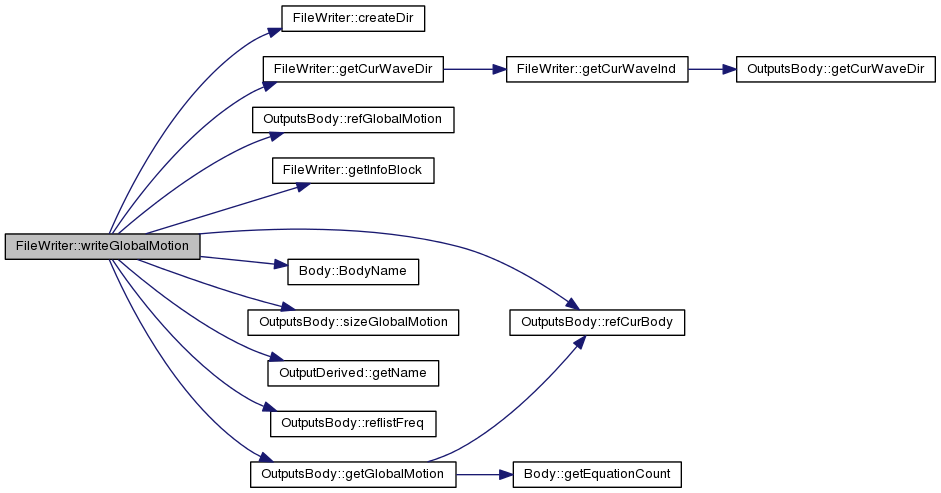
\includegraphics[width=350pt]{class_file_writer_a5c921b5ae92039cf50458e2c46e204da_cgraph}
\end{center}
\end{figure}


\hypertarget{class_file_writer_a317649499b8c16dd529e2bf588e3be88}{\index{File\-Writer@{File\-Writer}!write\-Global\-Solution@{write\-Global\-Solution}}
\index{write\-Global\-Solution@{write\-Global\-Solution}!FileWriter@{File\-Writer}}
\subsubsection[{write\-Global\-Solution}]{\setlength{\rightskip}{0pt plus 5cm}bool File\-Writer\-::write\-Global\-Solution (
\begin{DoxyParamCaption}
{}
\end{DoxyParamCaption}
)}}\label{class_file_writer_a317649499b8c16dd529e2bf588e3be88}


Writes the output file of global solutions. If file exists, appends to the file, assuming the appended file is a new body object. 

\begin{DoxyReturn}{Returns}
Returns true if write successful. 
\end{DoxyReturn}


Here is the call graph for this function\-:\nopagebreak
\begin{figure}[H]
\begin{center}
\leavevmode
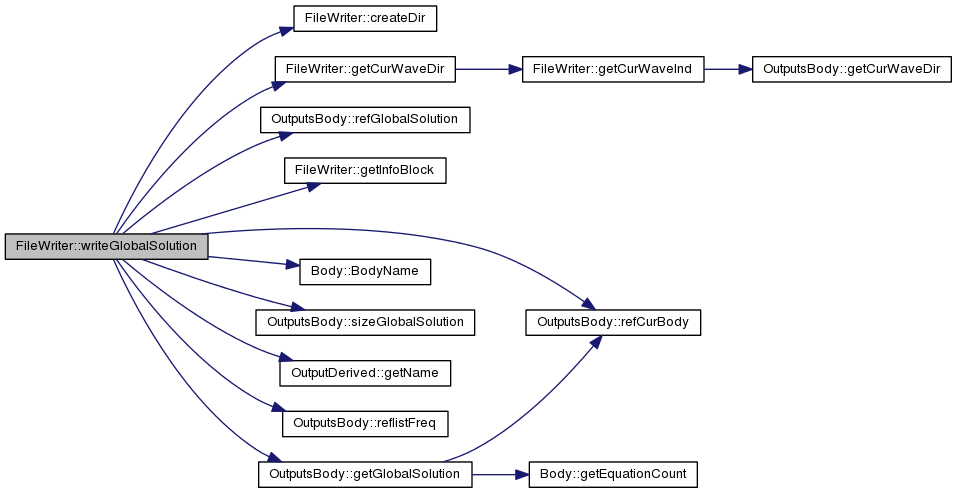
\includegraphics[width=350pt]{class_file_writer_a317649499b8c16dd529e2bf588e3be88_cgraph}
\end{center}
\end{figure}


\hypertarget{class_file_writer_a2078a50dbd21946aeed86d8e0bccd50e}{\index{File\-Writer@{File\-Writer}!write\-Global\-Velocity@{write\-Global\-Velocity}}
\index{write\-Global\-Velocity@{write\-Global\-Velocity}!FileWriter@{File\-Writer}}
\subsubsection[{write\-Global\-Velocity}]{\setlength{\rightskip}{0pt plus 5cm}bool File\-Writer\-::write\-Global\-Velocity (
\begin{DoxyParamCaption}
{}
\end{DoxyParamCaption}
)}}\label{class_file_writer_a2078a50dbd21946aeed86d8e0bccd50e}


Writes the output file of global velocities. If file exists, appends to the file, assuming the appended file is a new body object. 

\begin{DoxyReturn}{Returns}
Returns true if write successful. 
\end{DoxyReturn}


Here is the call graph for this function\-:\nopagebreak
\begin{figure}[H]
\begin{center}
\leavevmode
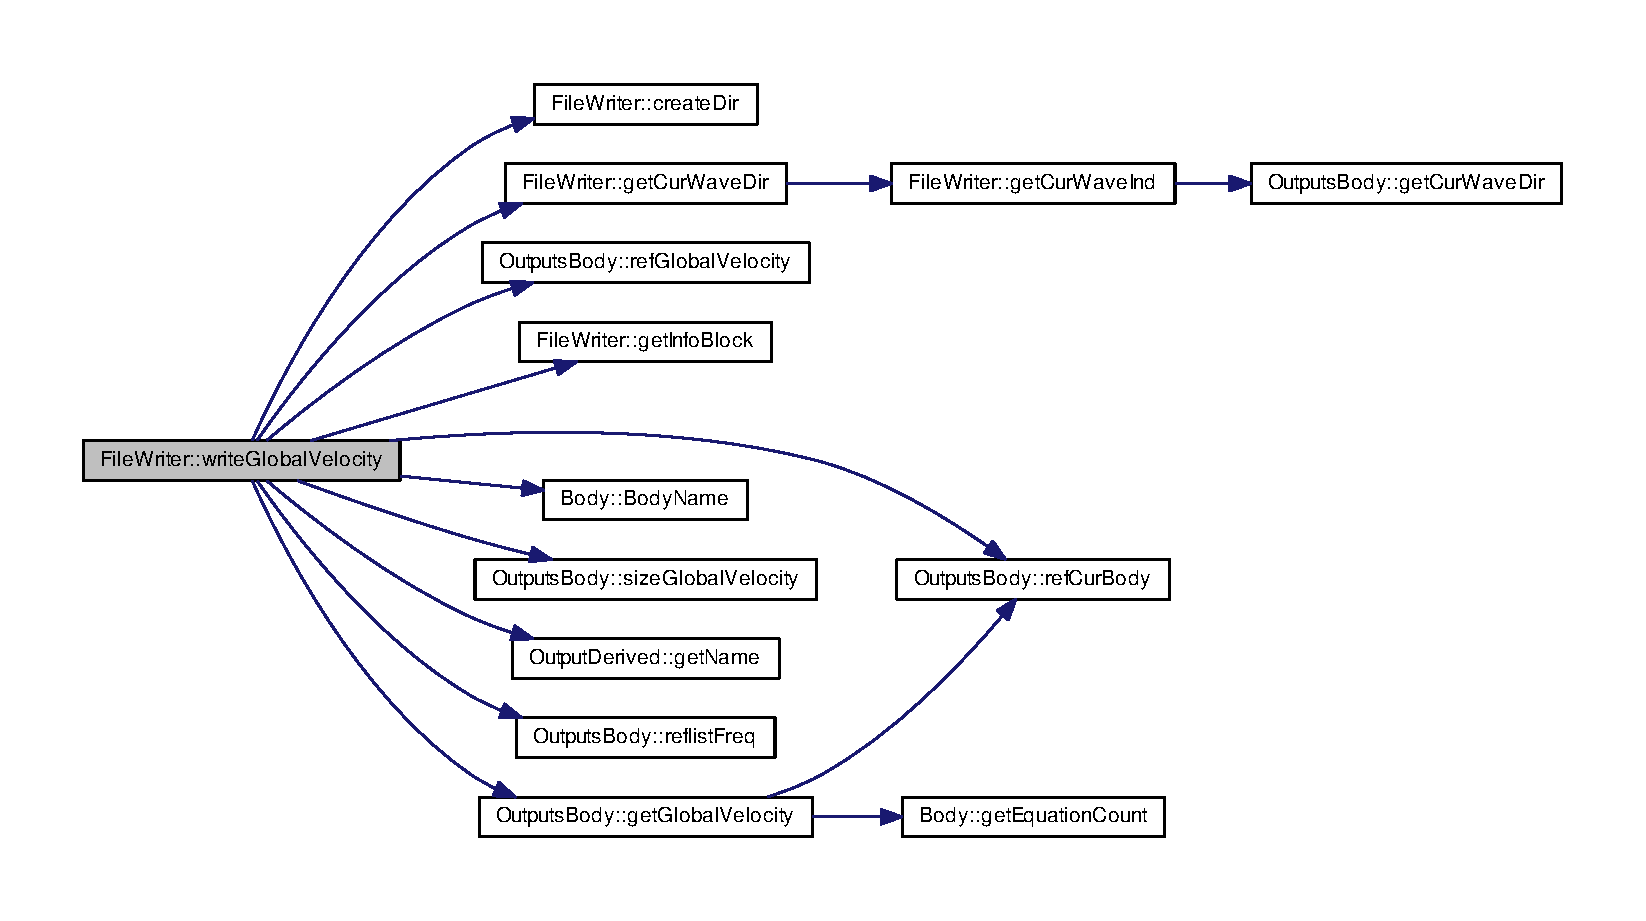
\includegraphics[width=350pt]{class_file_writer_a2078a50dbd21946aeed86d8e0bccd50e_cgraph}
\end{center}
\end{figure}


\hypertarget{class_file_writer_a0428a4f8ad72d01ff5316bfa3e4ce631}{\index{File\-Writer@{File\-Writer}!write\-Wave\-Direction@{write\-Wave\-Direction}}
\index{write\-Wave\-Direction@{write\-Wave\-Direction}!FileWriter@{File\-Writer}}
\subsubsection[{write\-Wave\-Direction}]{\setlength{\rightskip}{0pt plus 5cm}bool File\-Writer\-::write\-Wave\-Direction (
\begin{DoxyParamCaption}
{}
\end{DoxyParamCaption}
)}}\label{class_file_writer_a0428a4f8ad72d01ff5316bfa3e4ce631}


Writes the directions list to file. 

\begin{DoxyReturn}{Returns}
true if write successful. 
\end{DoxyReturn}


Here is the call graph for this function\-:\nopagebreak
\begin{figure}[H]
\begin{center}
\leavevmode
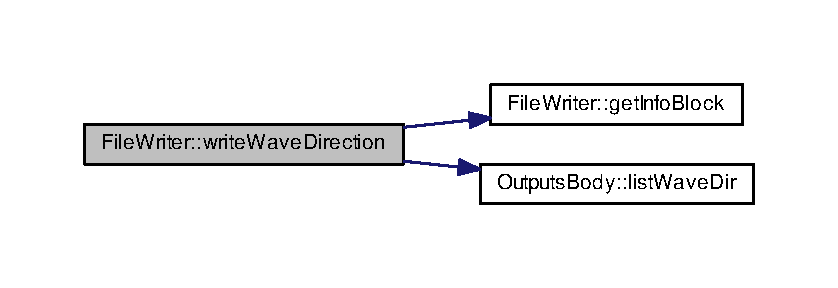
\includegraphics[width=350pt]{class_file_writer_a0428a4f8ad72d01ff5316bfa3e4ce631_cgraph}
\end{center}
\end{figure}




The documentation for this class was generated from the following files\-:\begin{DoxyCompactItemize}
\item 
/home/nicholas/\-Ship Design/\-Projects/\-D\-M\-S1305 Open\-S\-E\-A/master/200\-\_\-src/bin/ofreq/file\-\_\-writer/filewriter.\-h\item 
/home/nicholas/\-Ship Design/\-Projects/\-D\-M\-S1305 Open\-S\-E\-A/master/200\-\_\-src/bin/ofreq/file\-\_\-writer/filewriter.\-cpp\end{DoxyCompactItemize}

\hypertarget{class_force}{\section{Force Class Reference}
\label{class_force}\index{Force@{Force}}
}


{\ttfamily \#include $<$force.\-h$>$}

Inheritance diagram for Force\-:\begin{figure}[H]
\begin{center}
\leavevmode
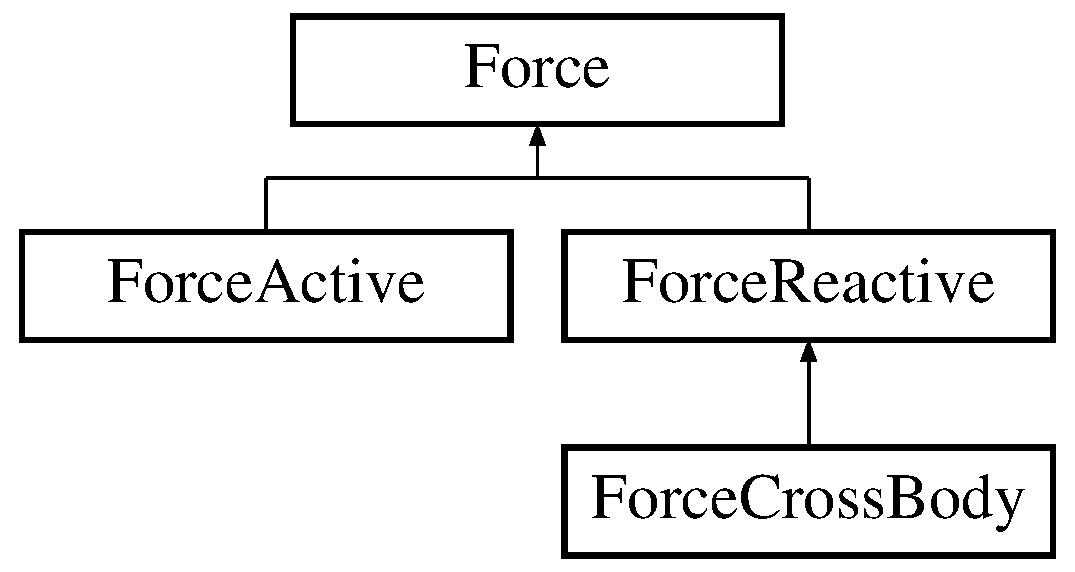
\includegraphics[height=3.000000cm]{class_force}
\end{center}
\end{figure}
\subsection*{Public Member Functions}
\begin{DoxyCompactItemize}
\item 
\hyperlink{class_force_a00983e3bbc206a00bb9253deafc4e424}{Force} ()
\item 
\hyperlink{class_force_a8767ca332cee738a462befe1bfbfa454}{$\sim$\-Force} ()
\item 
void \hyperlink{class_force_aefb0b71694f6ffbfe1ee06516f5536c3}{set\-Force\-Name} (string)
\item 
string \hyperlink{class_force_a8431fcc0edd27e3edb77f8176bec6908}{get\-Force\-Name} ()
\end{DoxyCompactItemize}
\subsection*{Protected Attributes}
\begin{DoxyCompactItemize}
\item 
string \hyperlink{class_force_a50b8739b17f549bd250936b0251ca571}{force\-Name}
\end{DoxyCompactItemize}


\subsection{Detailed Description}
This (base) class holds data for a force object. 

\subsection{Constructor \& Destructor Documentation}
\hypertarget{class_force_a00983e3bbc206a00bb9253deafc4e424}{\index{Force@{Force}!Force@{Force}}
\index{Force@{Force}!Force@{Force}}
\subsubsection[{Force}]{\setlength{\rightskip}{0pt plus 5cm}Force\-::\-Force (
\begin{DoxyParamCaption}
{}
\end{DoxyParamCaption}
)}}\label{class_force_a00983e3bbc206a00bb9253deafc4e424}
The default constructor. \hypertarget{class_force_a8767ca332cee738a462befe1bfbfa454}{\index{Force@{Force}!$\sim$\-Force@{$\sim$\-Force}}
\index{$\sim$\-Force@{$\sim$\-Force}!Force@{Force}}
\subsubsection[{$\sim$\-Force}]{\setlength{\rightskip}{0pt plus 5cm}Force\-::$\sim$\-Force (
\begin{DoxyParamCaption}
{}
\end{DoxyParamCaption}
)}}\label{class_force_a8767ca332cee738a462befe1bfbfa454}
The default destructor, nothing happens here. 

\subsection{Member Function Documentation}
\hypertarget{class_force_a8431fcc0edd27e3edb77f8176bec6908}{\index{Force@{Force}!get\-Force\-Name@{get\-Force\-Name}}
\index{get\-Force\-Name@{get\-Force\-Name}!Force@{Force}}
\subsubsection[{get\-Force\-Name}]{\setlength{\rightskip}{0pt plus 5cm}string Force\-::get\-Force\-Name (
\begin{DoxyParamCaption}
{}
\end{DoxyParamCaption}
)}}\label{class_force_a8431fcc0edd27e3edb77f8176bec6908}
Retrieve the name of the force. \begin{DoxyReturn}{Returns}
new\-Name The name of the force. 
\end{DoxyReturn}
\hypertarget{class_force_aefb0b71694f6ffbfe1ee06516f5536c3}{\index{Force@{Force}!set\-Force\-Name@{set\-Force\-Name}}
\index{set\-Force\-Name@{set\-Force\-Name}!Force@{Force}}
\subsubsection[{set\-Force\-Name}]{\setlength{\rightskip}{0pt plus 5cm}void Force\-::set\-Force\-Name (
\begin{DoxyParamCaption}
\item[{string}]{new\-Name}
\end{DoxyParamCaption}
)}}\label{class_force_aefb0b71694f6ffbfe1ee06516f5536c3}
Sets the name of the force. 
\begin{DoxyParams}{Parameters}
{\em new\-Name} & The name of the force. \\
\hline
\end{DoxyParams}


\subsection{Member Data Documentation}
\hypertarget{class_force_a50b8739b17f549bd250936b0251ca571}{\index{Force@{Force}!force\-Name@{force\-Name}}
\index{force\-Name@{force\-Name}!Force@{Force}}
\subsubsection[{force\-Name}]{\setlength{\rightskip}{0pt plus 5cm}string Force\-::force\-Name\hspace{0.3cm}{\ttfamily [protected]}}}\label{class_force_a50b8739b17f549bd250936b0251ca571}
The force name. 

The documentation for this class was generated from the following files\-:\begin{DoxyCompactItemize}
\item 
Visual Studio 2010/\-Projects/o\-Freq Windows V\-S2010/o\-Freq/force.\-h\item 
Visual Studio 2010/\-Projects/o\-Freq Windows V\-S2010/o\-Freq/force.\-cpp\end{DoxyCompactItemize}

\hypertarget{class_force_active}{\section{Force\-Active Class Reference}
\label{class_force_active}\index{Force\-Active@{Force\-Active}}
}


{\ttfamily \#include $<$forceactive.\-h$>$}



Inheritance diagram for Force\-Active\-:\nopagebreak
\begin{figure}[H]
\begin{center}
\leavevmode
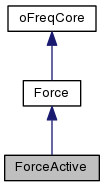
\includegraphics[width=150pt]{class_force_active__inherit__graph}
\end{center}
\end{figure}


Collaboration diagram for Force\-Active\-:\nopagebreak
\begin{figure}[H]
\begin{center}
\leavevmode
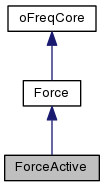
\includegraphics[width=150pt]{class_force_active__coll__graph}
\end{center}
\end{figure}
\subsection*{Public Member Functions}
\begin{DoxyCompactItemize}
\item 
\hyperlink{class_force_active_ae006e3394f8c925c6a3218686c5cc8ae}{Force\-Active} ()
\item 
virtual \hyperlink{class_force_active_aa2db4bc1fb74ecb6e0ee46c59a40dd2a}{$\sim$\-Force\-Active} ()
\item 
void \hyperlink{class_force_active_a1775530282b1d473cd95afd7f01619bb}{set\-Coeff} (complex$<$ double $>$ coeff\-In, unsigned int index)
\begin{DoxyCompactList}\small\item\em Sets the coefficient for the specified index. \end{DoxyCompactList}\item 
vector$<$ complex\-Double $>$ \& \hyperlink{class_force_active_a752a48e1f4dfc483a1cdb18754f8e630}{list\-Coefficients} ()
\item 
complex\-Double \& \hyperlink{class_force_active_af96d4a0a2f0aa28911d8798f62d3b8bd}{list\-Coefficients} (unsigned int index)
\begin{DoxyCompactList}\small\item\em Provides direct access to a coefficient from the list of coefficients. \end{DoxyCompactList}\item 
vector$<$ complex\-Double $>$ \& \hyperlink{class_force_active_a931628f3a5c5d9b142726697a96e1407}{list\-Equation} ()
\begin{DoxyCompactList}\small\item\em Another implementation of function list\-Coefficients. \end{DoxyCompactList}\item 
complex\-Double \& \hyperlink{class_force_active_a573a98979938dd6bfbaf5d40ae17a058}{list\-Equation} (unsigned int index)
\begin{DoxyCompactList}\small\item\em Another implementation of function list\-Coefficients(index). \end{DoxyCompactList}\item 
complex\-Double \hyperlink{class_force_active_a2e01f54c3071d2f8831fb7763cf14500}{get\-Equation} (int number)
\begin{DoxyCompactList}\small\item\em Get a specific number from the list of coefficients. \end{DoxyCompactList}\end{DoxyCompactItemize}
\subsection*{Protected Attributes}
\begin{DoxyCompactItemize}
\item 
vector$<$ complex\-Double $>$ \hyperlink{class_force_active_a8850c1b1145e5eb76f7d545466ef0ec6}{p\-Coefficients}
\end{DoxyCompactItemize}
\subsection*{Additional Inherited Members}


\subsection{Detailed Description}
This class holds data for an active force. 

\subsection{Constructor \& Destructor Documentation}
\hypertarget{class_force_active_ae006e3394f8c925c6a3218686c5cc8ae}{\index{Force\-Active@{Force\-Active}!Force\-Active@{Force\-Active}}
\index{Force\-Active@{Force\-Active}!ForceActive@{Force\-Active}}
\subsubsection[{Force\-Active}]{\setlength{\rightskip}{0pt plus 5cm}Force\-Active\-::\-Force\-Active (
\begin{DoxyParamCaption}
{}
\end{DoxyParamCaption}
)}}\label{class_force_active_ae006e3394f8c925c6a3218686c5cc8ae}
The default constructor. \hypertarget{class_force_active_aa2db4bc1fb74ecb6e0ee46c59a40dd2a}{\index{Force\-Active@{Force\-Active}!$\sim$\-Force\-Active@{$\sim$\-Force\-Active}}
\index{$\sim$\-Force\-Active@{$\sim$\-Force\-Active}!ForceActive@{Force\-Active}}
\subsubsection[{$\sim$\-Force\-Active}]{\setlength{\rightskip}{0pt plus 5cm}Force\-Active\-::$\sim$\-Force\-Active (
\begin{DoxyParamCaption}
{}
\end{DoxyParamCaption}
)\hspace{0.3cm}{\ttfamily [virtual]}}}\label{class_force_active_aa2db4bc1fb74ecb6e0ee46c59a40dd2a}
The default destructor, nothing happens here. 

\subsection{Member Function Documentation}
\hypertarget{class_force_active_a2e01f54c3071d2f8831fb7763cf14500}{\index{Force\-Active@{Force\-Active}!get\-Equation@{get\-Equation}}
\index{get\-Equation@{get\-Equation}!ForceActive@{Force\-Active}}
\subsubsection[{get\-Equation}]{\setlength{\rightskip}{0pt plus 5cm}complex\-Double Force\-Active\-::get\-Equation (
\begin{DoxyParamCaption}
\item[{int}]{number}
\end{DoxyParamCaption}
)}}\label{class_force_active_a2e01f54c3071d2f8831fb7763cf14500}


Get a specific number from the list of coefficients. 

Get a specific number from the list of coefficients. Similar to get\-Coefficients(), only instead of returning the entire vector of coefficients, this only returns a single value in the list. 
\begin{DoxyParams}{Parameters}
{\em number} & Integer specifying which number should be retrieved from the list. \\
\hline
\end{DoxyParams}
\begin{DoxyReturn}{Returns}
Complex Double which is the input coefficient for the active force on the equation specified by number. Returns by value, not by reference. 
\end{DoxyReturn}
\hypertarget{class_force_active_a752a48e1f4dfc483a1cdb18754f8e630}{\index{Force\-Active@{Force\-Active}!list\-Coefficients@{list\-Coefficients}}
\index{list\-Coefficients@{list\-Coefficients}!ForceActive@{Force\-Active}}
\subsubsection[{list\-Coefficients}]{\setlength{\rightskip}{0pt plus 5cm}vector$<$ complex\-Double $>$ \& Force\-Active\-::list\-Coefficients (
\begin{DoxyParamCaption}
{}
\end{DoxyParamCaption}
)}}\label{class_force_active_a752a48e1f4dfc483a1cdb18754f8e630}
Retrieve the list of coefficients. \begin{DoxyReturn}{Returns}
The list of coefficients. 
\end{DoxyReturn}


Here is the caller graph for this function\-:
\nopagebreak
\begin{figure}[H]
\begin{center}
\leavevmode
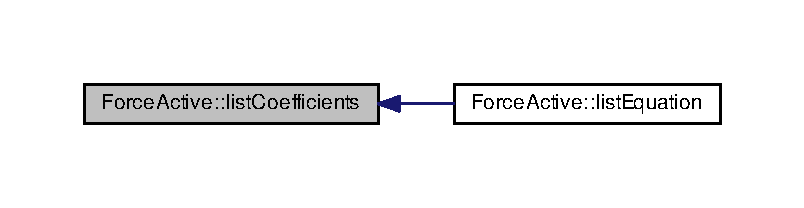
\includegraphics[width=350pt]{class_force_active_a752a48e1f4dfc483a1cdb18754f8e630_icgraph}
\end{center}
\end{figure}


\hypertarget{class_force_active_af96d4a0a2f0aa28911d8798f62d3b8bd}{\index{Force\-Active@{Force\-Active}!list\-Coefficients@{list\-Coefficients}}
\index{list\-Coefficients@{list\-Coefficients}!ForceActive@{Force\-Active}}
\subsubsection[{list\-Coefficients}]{\setlength{\rightskip}{0pt plus 5cm}complex\-Double \& Force\-Active\-::list\-Coefficients (
\begin{DoxyParamCaption}
\item[{unsigned int}]{index}
\end{DoxyParamCaption}
)}}\label{class_force_active_af96d4a0a2f0aa28911d8798f62d3b8bd}


Provides direct access to a coefficient from the list of coefficients. 

Returns a value from the list of coefficents. Which value to return is specified by the input index. 
\begin{DoxyParams}{Parameters}
{\em index} & Unsigned integer. Specifies which value to return from the list of coefficients. \\
\hline
\end{DoxyParams}
\begin{DoxyReturn}{Returns}
Returns a complex double. Returned variable is a value from the list of coefficients. Returned variable is passed by reference. 
\end{DoxyReturn}
\hypertarget{class_force_active_a931628f3a5c5d9b142726697a96e1407}{\index{Force\-Active@{Force\-Active}!list\-Equation@{list\-Equation}}
\index{list\-Equation@{list\-Equation}!ForceActive@{Force\-Active}}
\subsubsection[{list\-Equation}]{\setlength{\rightskip}{0pt plus 5cm}vector$<$ complex\-Double $>$ \& Force\-Active\-::list\-Equation (
\begin{DoxyParamCaption}
{}
\end{DoxyParamCaption}
)}}\label{class_force_active_a931628f3a5c5d9b142726697a96e1407}


Another implementation of function list\-Coefficients. 

\begin{DoxyReturn}{Returns}
Vector containing the list of coefficients. Argument passed by reference. 
\end{DoxyReturn}


Here is the call graph for this function\-:
\nopagebreak
\begin{figure}[H]
\begin{center}
\leavevmode
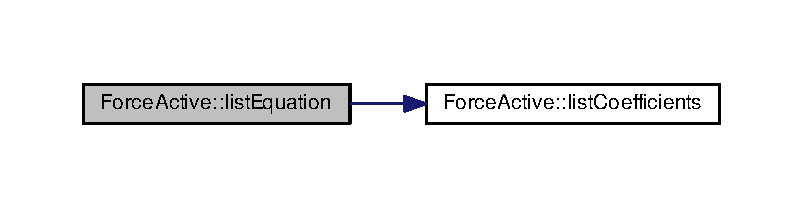
\includegraphics[width=350pt]{class_force_active_a931628f3a5c5d9b142726697a96e1407_cgraph}
\end{center}
\end{figure}


\hypertarget{class_force_active_a573a98979938dd6bfbaf5d40ae17a058}{\index{Force\-Active@{Force\-Active}!list\-Equation@{list\-Equation}}
\index{list\-Equation@{list\-Equation}!ForceActive@{Force\-Active}}
\subsubsection[{list\-Equation}]{\setlength{\rightskip}{0pt plus 5cm}complex\-Double \& Force\-Active\-::list\-Equation (
\begin{DoxyParamCaption}
\item[{unsigned int}]{index}
\end{DoxyParamCaption}
)}}\label{class_force_active_a573a98979938dd6bfbaf5d40ae17a058}


Another implementation of function list\-Coefficients(index). 

Provides direct access to items in the list of equations. Returns a single variable from the list of coefficients. 
\begin{DoxyParams}{Parameters}
{\em index} & Unsigned integer. Specifies which value to return from the list of coefficients. \\
\hline
\end{DoxyParams}
\begin{DoxyReturn}{Returns}
Returns a complex double. Returned variable is a value from the list of coefficients. Returned variable is passed by reference. 
\end{DoxyReturn}


Here is the call graph for this function\-:
\nopagebreak
\begin{figure}[H]
\begin{center}
\leavevmode
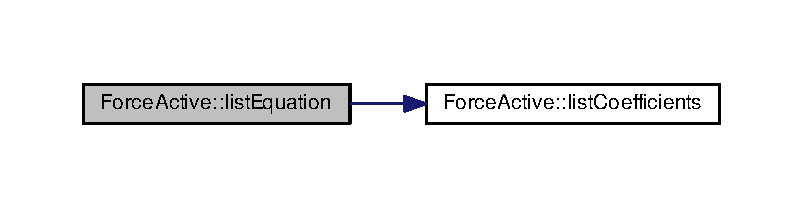
\includegraphics[width=350pt]{class_force_active_a573a98979938dd6bfbaf5d40ae17a058_cgraph}
\end{center}
\end{figure}


\hypertarget{class_force_active_a1775530282b1d473cd95afd7f01619bb}{\index{Force\-Active@{Force\-Active}!set\-Coeff@{set\-Coeff}}
\index{set\-Coeff@{set\-Coeff}!ForceActive@{Force\-Active}}
\subsubsection[{set\-Coeff}]{\setlength{\rightskip}{0pt plus 5cm}void Force\-Active\-::set\-Coeff (
\begin{DoxyParamCaption}
\item[{complex$<$ double $>$}]{coeff\-In, }
\item[{unsigned int}]{index}
\end{DoxyParamCaption}
)}}\label{class_force_active_a1775530282b1d473cd95afd7f01619bb}


Sets the coefficient for the specified index. 


\begin{DoxyParams}{Parameters}
{\em coeff\-In} & The value of the coefficient to specify. Added as a complex number. Variable passed by value. \\
\hline
{\em index} & The equation index of the coefficient to specify. \\
\hline
\end{DoxyParams}


\subsection{Member Data Documentation}
\hypertarget{class_force_active_a8850c1b1145e5eb76f7d545466ef0ec6}{\index{Force\-Active@{Force\-Active}!p\-Coefficients@{p\-Coefficients}}
\index{p\-Coefficients@{p\-Coefficients}!ForceActive@{Force\-Active}}
\subsubsection[{p\-Coefficients}]{\setlength{\rightskip}{0pt plus 5cm}vector$<$complex\-Double$>$ Force\-Active\-::p\-Coefficients\hspace{0.3cm}{\ttfamily [protected]}}}\label{class_force_active_a8850c1b1145e5eb76f7d545466ef0ec6}
The list of force coeffients. 

The documentation for this class was generated from the following files\-:\begin{DoxyCompactItemize}
\item 
forceactive.\-h\item 
forceactive.\-cpp\end{DoxyCompactItemize}

\hypertarget{class_force_cross_body}{\section{Force\-Cross\-Body Class Reference}
\label{class_force_cross_body}\index{Force\-Cross\-Body@{Force\-Cross\-Body}}
}


{\ttfamily \#include $<$forcecrossbody.\-h$>$}

Inheritance diagram for Force\-Cross\-Body\-:\begin{figure}[H]
\begin{center}
\leavevmode
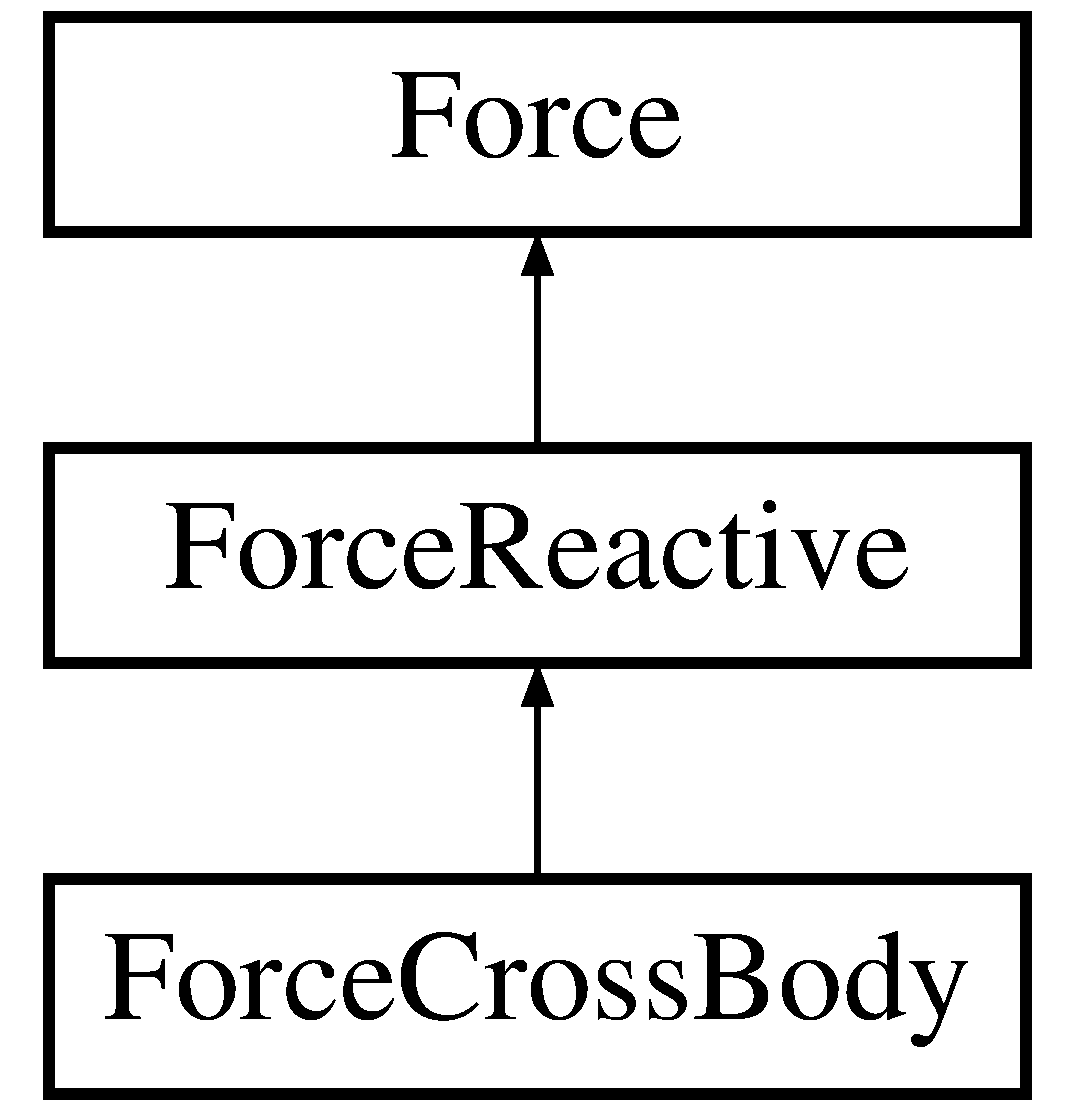
\includegraphics[height=3.000000cm]{class_force_cross_body}
\end{center}
\end{figure}
\subsection*{Public Member Functions}
\begin{DoxyCompactItemize}
\item 
\hyperlink{class_force_cross_body_a722c4ffad05245be224190bde22c6607}{Force\-Cross\-Body} ()
\item 
\hyperlink{class_force_cross_body_aaac5e33c56dcd4aee27f1e5ce1a0afa5}{$\sim$\-Force\-Cross\-Body} ()
\item 
void \hyperlink{class_force_cross_body_ab6bb83f04e9eec3b537b2570d712b3f8}{test\-Print} ()
\end{DoxyCompactItemize}
\subsection*{Additional Inherited Members}


\subsection{Detailed Description}
This class holds data for a cross body force. 

\subsection{Constructor \& Destructor Documentation}
\hypertarget{class_force_cross_body_a722c4ffad05245be224190bde22c6607}{\index{Force\-Cross\-Body@{Force\-Cross\-Body}!Force\-Cross\-Body@{Force\-Cross\-Body}}
\index{Force\-Cross\-Body@{Force\-Cross\-Body}!ForceCrossBody@{Force\-Cross\-Body}}
\subsubsection[{Force\-Cross\-Body}]{\setlength{\rightskip}{0pt plus 5cm}Force\-Cross\-Body\-::\-Force\-Cross\-Body (
\begin{DoxyParamCaption}
{}
\end{DoxyParamCaption}
)}}\label{class_force_cross_body_a722c4ffad05245be224190bde22c6607}
This default constructor creates a \hyperlink{class_body}{Body} object. \hypertarget{class_force_cross_body_aaac5e33c56dcd4aee27f1e5ce1a0afa5}{\index{Force\-Cross\-Body@{Force\-Cross\-Body}!$\sim$\-Force\-Cross\-Body@{$\sim$\-Force\-Cross\-Body}}
\index{$\sim$\-Force\-Cross\-Body@{$\sim$\-Force\-Cross\-Body}!ForceCrossBody@{Force\-Cross\-Body}}
\subsubsection[{$\sim$\-Force\-Cross\-Body}]{\setlength{\rightskip}{0pt plus 5cm}Force\-Cross\-Body\-::$\sim$\-Force\-Cross\-Body (
\begin{DoxyParamCaption}
{}
\end{DoxyParamCaption}
)}}\label{class_force_cross_body_aaac5e33c56dcd4aee27f1e5ce1a0afa5}
The default destructor, nothing happens here. 

\subsection{Member Function Documentation}
\hypertarget{class_force_cross_body_ab6bb83f04e9eec3b537b2570d712b3f8}{\index{Force\-Cross\-Body@{Force\-Cross\-Body}!test\-Print@{test\-Print}}
\index{test\-Print@{test\-Print}!ForceCrossBody@{Force\-Cross\-Body}}
\subsubsection[{test\-Print}]{\setlength{\rightskip}{0pt plus 5cm}void Force\-Cross\-Body\-::test\-Print (
\begin{DoxyParamCaption}
{}
\end{DoxyParamCaption}
)}}\label{class_force_cross_body_ab6bb83f04e9eec3b537b2570d712b3f8}
Test print to console the values of all data members. 

The documentation for this class was generated from the following files\-:\begin{DoxyCompactItemize}
\item 
Visual Studio 2010/\-Projects/o\-Freq Windows V\-S2010/o\-Freq/forcecrossbody.\-h\item 
Visual Studio 2010/\-Projects/o\-Freq Windows V\-S2010/o\-Freq/forcecrossbody.\-cpp\end{DoxyCompactItemize}

\hypertarget{class_force_reactive}{\section{Force\-Reactive Class Reference}
\label{class_force_reactive}\index{Force\-Reactive@{Force\-Reactive}}
}


{\ttfamily \#include $<$forcereactive.\-h$>$}

Inheritance diagram for Force\-Reactive\-:\begin{figure}[H]
\begin{center}
\leavevmode
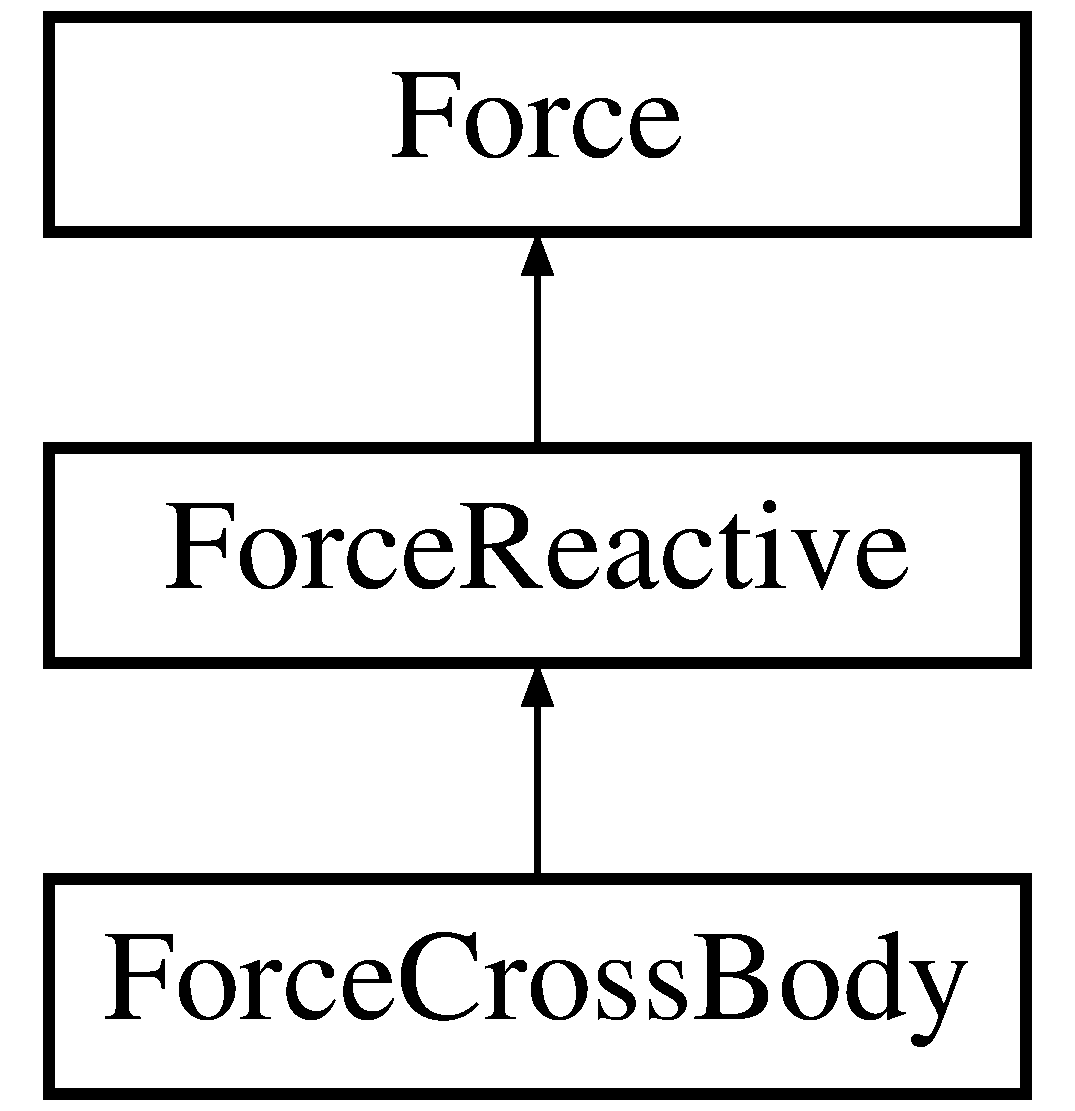
\includegraphics[height=3.000000cm]{class_force_reactive}
\end{center}
\end{figure}
\subsection*{Public Member Functions}
\begin{DoxyCompactItemize}
\item 
\hyperlink{class_force_reactive_a620cb084872d0d7e1c5d596fc05b00e5}{Force\-Reactive} ()
\item 
\hyperlink{class_force_reactive_abb3aceb796c02f9289b6b270a36d1a9d}{$\sim$\-Force\-Reactive} ()
\item 
void \hyperlink{class_force_reactive_adc057ed59345c6f7a8f522e80ab9be08}{test\-Print} ()
\item 
void \hyperlink{class_force_reactive_a2594a1dd03dd983e7eb4204148698c34}{set\-Coeff} (vector$<$ string $>$, bool)
\item 
void \hyperlink{class_force_reactive_a6f1969b59143d74dfd05006dcb18414d}{set\-Cur\-Derivative} (int)
\item 
void \hyperlink{class_force_reactive_a6e1a59348fb32dc15a6918bfc42a4cad}{set\-Cur\-Equation\-Num} (int)
\item 
vector$<$ \hyperlink{class_derivative}{Derivative} $>$ \hyperlink{class_force_reactive_aff4ed3ee3ba6ff0b013fb02183c01af8}{get\-Derivatives} ()
\end{DoxyCompactItemize}
\subsection*{Protected Attributes}
\begin{DoxyCompactItemize}
\item 
\hyperlink{class_derivative}{Derivative} \hyperlink{class_force_reactive_ad0da544a781cfac29d317e8c59e9f3f0}{derivative} \mbox{[}M\-A\-X\-\_\-\-O\-R\-D\-E\-R\-\_\-\-D\-E\-R\-I\-V\-A\-T\-I\-V\-E\mbox{]}
\item 
int \hyperlink{class_force_reactive_a6c4302050614499c9ffeda4ad21928ec}{current\-Derivative}
\item 
int \hyperlink{class_force_reactive_a9aa1f30d63006bc56be33830da1d8331}{current\-Equation}
\end{DoxyCompactItemize}


\subsection{Detailed Description}
This class holds all of the data for a reactive force. 

\subsection{Constructor \& Destructor Documentation}
\hypertarget{class_force_reactive_a620cb084872d0d7e1c5d596fc05b00e5}{\index{Force\-Reactive@{Force\-Reactive}!Force\-Reactive@{Force\-Reactive}}
\index{Force\-Reactive@{Force\-Reactive}!ForceReactive@{Force\-Reactive}}
\subsubsection[{Force\-Reactive}]{\setlength{\rightskip}{0pt plus 5cm}Force\-Reactive\-::\-Force\-Reactive (
\begin{DoxyParamCaption}
{}
\end{DoxyParamCaption}
)}}\label{class_force_reactive_a620cb084872d0d7e1c5d596fc05b00e5}
This default constructor. \hypertarget{class_force_reactive_abb3aceb796c02f9289b6b270a36d1a9d}{\index{Force\-Reactive@{Force\-Reactive}!$\sim$\-Force\-Reactive@{$\sim$\-Force\-Reactive}}
\index{$\sim$\-Force\-Reactive@{$\sim$\-Force\-Reactive}!ForceReactive@{Force\-Reactive}}
\subsubsection[{$\sim$\-Force\-Reactive}]{\setlength{\rightskip}{0pt plus 5cm}Force\-Reactive\-::$\sim$\-Force\-Reactive (
\begin{DoxyParamCaption}
{}
\end{DoxyParamCaption}
)}}\label{class_force_reactive_abb3aceb796c02f9289b6b270a36d1a9d}
The default destructor, nothing happens here. 

\subsection{Member Function Documentation}
\hypertarget{class_force_reactive_aff4ed3ee3ba6ff0b013fb02183c01af8}{\index{Force\-Reactive@{Force\-Reactive}!get\-Derivatives@{get\-Derivatives}}
\index{get\-Derivatives@{get\-Derivatives}!ForceReactive@{Force\-Reactive}}
\subsubsection[{get\-Derivatives}]{\setlength{\rightskip}{0pt plus 5cm}vector$<$ {\bf Derivative} $>$ Force\-Reactive\-::get\-Derivatives (
\begin{DoxyParamCaption}
{}
\end{DoxyParamCaption}
)}}\label{class_force_reactive_aff4ed3ee3ba6ff0b013fb02183c01af8}
Retrieve the order derivative \begin{DoxyReturn}{Returns}
The order derivative of this object. 
\end{DoxyReturn}
\hypertarget{class_force_reactive_a2594a1dd03dd983e7eb4204148698c34}{\index{Force\-Reactive@{Force\-Reactive}!set\-Coeff@{set\-Coeff}}
\index{set\-Coeff@{set\-Coeff}!ForceReactive@{Force\-Reactive}}
\subsubsection[{set\-Coeff}]{\setlength{\rightskip}{0pt plus 5cm}void Force\-Reactive\-::set\-Coeff (
\begin{DoxyParamCaption}
\item[{vector$<$ string $>$}]{new\-List, }
\item[{bool}]{is\-Direct\-List}
\end{DoxyParamCaption}
)}}\label{class_force_reactive_a2594a1dd03dd983e7eb4204148698c34}
Sets the list of coeffcients. 
\begin{DoxyParams}{Parameters}
{\em new\-List} & The list of coefficients. \\
\hline
{\em is\-Direct\-List} & Specifies whether the list is direct or sequential. \\
\hline
\end{DoxyParams}
\hypertarget{class_force_reactive_a6f1969b59143d74dfd05006dcb18414d}{\index{Force\-Reactive@{Force\-Reactive}!set\-Cur\-Derivative@{set\-Cur\-Derivative}}
\index{set\-Cur\-Derivative@{set\-Cur\-Derivative}!ForceReactive@{Force\-Reactive}}
\subsubsection[{set\-Cur\-Derivative}]{\setlength{\rightskip}{0pt plus 5cm}void Force\-Reactive\-::set\-Cur\-Derivative (
\begin{DoxyParamCaption}
\item[{int}]{new\-Order}
\end{DoxyParamCaption}
)}}\label{class_force_reactive_a6f1969b59143d74dfd05006dcb18414d}
Sets the current derivative. 
\begin{DoxyParams}{Parameters}
{\em neworder} & The order of derivative. \\
\hline
\end{DoxyParams}
\hypertarget{class_force_reactive_a6e1a59348fb32dc15a6918bfc42a4cad}{\index{Force\-Reactive@{Force\-Reactive}!set\-Cur\-Equation\-Num@{set\-Cur\-Equation\-Num}}
\index{set\-Cur\-Equation\-Num@{set\-Cur\-Equation\-Num}!ForceReactive@{Force\-Reactive}}
\subsubsection[{set\-Cur\-Equation\-Num}]{\setlength{\rightskip}{0pt plus 5cm}void Force\-Reactive\-::set\-Cur\-Equation\-Num (
\begin{DoxyParamCaption}
\item[{int}]{new\-Equation\-Num}
\end{DoxyParamCaption}
)}}\label{class_force_reactive_a6e1a59348fb32dc15a6918bfc42a4cad}
Sets the current number of the equation. 
\begin{DoxyParams}{Parameters}
{\em new\-Equation\-Num} & The number of the equation. \\
\hline
\end{DoxyParams}
\hypertarget{class_force_reactive_adc057ed59345c6f7a8f522e80ab9be08}{\index{Force\-Reactive@{Force\-Reactive}!test\-Print@{test\-Print}}
\index{test\-Print@{test\-Print}!ForceReactive@{Force\-Reactive}}
\subsubsection[{test\-Print}]{\setlength{\rightskip}{0pt plus 5cm}void Force\-Reactive\-::test\-Print (
\begin{DoxyParamCaption}
{}
\end{DoxyParamCaption}
)}}\label{class_force_reactive_adc057ed59345c6f7a8f522e80ab9be08}
Test print to console the values of all data members. 

\subsection{Member Data Documentation}
\hypertarget{class_force_reactive_a6c4302050614499c9ffeda4ad21928ec}{\index{Force\-Reactive@{Force\-Reactive}!current\-Derivative@{current\-Derivative}}
\index{current\-Derivative@{current\-Derivative}!ForceReactive@{Force\-Reactive}}
\subsubsection[{current\-Derivative}]{\setlength{\rightskip}{0pt plus 5cm}int Force\-Reactive\-::current\-Derivative\hspace{0.3cm}{\ttfamily [protected]}}}\label{class_force_reactive_a6c4302050614499c9ffeda4ad21928ec}
The current order derivative. \hypertarget{class_force_reactive_a9aa1f30d63006bc56be33830da1d8331}{\index{Force\-Reactive@{Force\-Reactive}!current\-Equation@{current\-Equation}}
\index{current\-Equation@{current\-Equation}!ForceReactive@{Force\-Reactive}}
\subsubsection[{current\-Equation}]{\setlength{\rightskip}{0pt plus 5cm}int Force\-Reactive\-::current\-Equation\hspace{0.3cm}{\ttfamily [protected]}}}\label{class_force_reactive_a9aa1f30d63006bc56be33830da1d8331}
This current equation number. \hypertarget{class_force_reactive_ad0da544a781cfac29d317e8c59e9f3f0}{\index{Force\-Reactive@{Force\-Reactive}!derivative@{derivative}}
\index{derivative@{derivative}!ForceReactive@{Force\-Reactive}}
\subsubsection[{derivative}]{\setlength{\rightskip}{0pt plus 5cm}{\bf Derivative} Force\-Reactive\-::derivative\mbox{[}M\-A\-X\-\_\-\-O\-R\-D\-E\-R\-\_\-\-D\-E\-R\-I\-V\-A\-T\-I\-V\-E\mbox{]}\hspace{0.3cm}{\ttfamily [protected]}}}\label{class_force_reactive_ad0da544a781cfac29d317e8c59e9f3f0}
This list of derivatives. 

The documentation for this class was generated from the following files\-:\begin{DoxyCompactItemize}
\item 
Visual Studio 2010/\-Projects/o\-Freq Windows V\-S2010/o\-Freq/forcereactive.\-h\item 
Visual Studio 2010/\-Projects/o\-Freq Windows V\-S2010/o\-Freq/forcereactive.\-cpp\end{DoxyCompactItemize}

\hypertarget{class_forces_input}{\section{Forces\-Input Class Reference}
\label{class_forces_input}\index{Forces\-Input@{Forces\-Input}}
}


{\ttfamily \#include $<$forcesinput.\-h$>$}



Inheritance diagram for Forces\-Input\-:\nopagebreak
\begin{figure}[H]
\begin{center}
\leavevmode
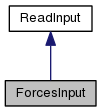
\includegraphics[width=148pt]{class_forces_input__inherit__graph}
\end{center}
\end{figure}


Collaboration diagram for Forces\-Input\-:\nopagebreak
\begin{figure}[H]
\begin{center}
\leavevmode
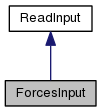
\includegraphics[width=148pt]{class_forces_input__coll__graph}
\end{center}
\end{figure}
\subsection*{Public Member Functions}
\begin{DoxyCompactItemize}
\item 
\hyperlink{class_forces_input_ad3da9dd7decddd74ba054f3e58a848fe}{Forces\-Input} ()
\item 
\hyperlink{class_forces_input_a5891d1dd81b2e4202fe023985aa0ff1b}{$\sim$\-Forces\-Input} ()
\item 
void \hyperlink{class_forces_input_af9ca173b1f53914ba8f118ae2cc211a3}{test\-Print} ()
\item 
User\-Forces \hyperlink{class_forces_input_ab5262ae1b53c658dbaab66d338e465e2}{get\-User\-Forces} ()
\end{DoxyCompactItemize}
\subsection*{Protected Member Functions}
\begin{DoxyCompactItemize}
\item 
void \hyperlink{class_forces_input_a8bcfe50a80d1c2fe11a742081a5e7343}{initialize\-Defaults} ()
\item 
int \hyperlink{class_forces_input_a5f4086acc636b54b64bcd611bdff1aa4}{legal\-Keyword} (string)
\item 
bool \hyperlink{class_forces_input_a3e82ee7aa3c5bd35a6bb1b06fcafafa9}{keyword\-Handler} (int, string, string)
\item 
bool \hyperlink{class_forces_input_a52965f2bfde734252e7f4f65bf0fde25}{keyword\-Handler} (int, vector$<$ string $>$, bool)
\end{DoxyCompactItemize}


\subsection{Detailed Description}
This class parses input from file and stores the data appropriately in the User\-Forces object. 

\subsection{Constructor \& Destructor Documentation}
\hypertarget{class_forces_input_ad3da9dd7decddd74ba054f3e58a848fe}{\index{Forces\-Input@{Forces\-Input}!Forces\-Input@{Forces\-Input}}
\index{Forces\-Input@{Forces\-Input}!ForcesInput@{Forces\-Input}}
\subsubsection[{Forces\-Input}]{\setlength{\rightskip}{0pt plus 5cm}Forces\-Input\-::\-Forces\-Input (
\begin{DoxyParamCaption}
{}
\end{DoxyParamCaption}
)}}\label{class_forces_input_ad3da9dd7decddd74ba054f3e58a848fe}
The default constructor. \hypertarget{class_forces_input_a5891d1dd81b2e4202fe023985aa0ff1b}{\index{Forces\-Input@{Forces\-Input}!$\sim$\-Forces\-Input@{$\sim$\-Forces\-Input}}
\index{$\sim$\-Forces\-Input@{$\sim$\-Forces\-Input}!ForcesInput@{Forces\-Input}}
\subsubsection[{$\sim$\-Forces\-Input}]{\setlength{\rightskip}{0pt plus 5cm}Forces\-Input\-::$\sim$\-Forces\-Input (
\begin{DoxyParamCaption}
{}
\end{DoxyParamCaption}
)}}\label{class_forces_input_a5891d1dd81b2e4202fe023985aa0ff1b}
The default destructor, nothing happens here. 

\subsection{Member Function Documentation}
\hypertarget{class_forces_input_ab5262ae1b53c658dbaab66d338e465e2}{\index{Forces\-Input@{Forces\-Input}!get\-User\-Forces@{get\-User\-Forces}}
\index{get\-User\-Forces@{get\-User\-Forces}!ForcesInput@{Forces\-Input}}
\subsubsection[{get\-User\-Forces}]{\setlength{\rightskip}{0pt plus 5cm}User\-Forces Forces\-Input\-::get\-User\-Forces (
\begin{DoxyParamCaption}
{}
\end{DoxyParamCaption}
)}}\label{class_forces_input_ab5262ae1b53c658dbaab66d338e465e2}
Returns user forces. \hypertarget{class_forces_input_a8bcfe50a80d1c2fe11a742081a5e7343}{\index{Forces\-Input@{Forces\-Input}!initialize\-Defaults@{initialize\-Defaults}}
\index{initialize\-Defaults@{initialize\-Defaults}!ForcesInput@{Forces\-Input}}
\subsubsection[{initialize\-Defaults}]{\setlength{\rightskip}{0pt plus 5cm}void Forces\-Input\-::initialize\-Defaults (
\begin{DoxyParamCaption}
{}
\end{DoxyParamCaption}
)\hspace{0.3cm}{\ttfamily [protected]}, {\ttfamily [virtual]}}}\label{class_forces_input_a8bcfe50a80d1c2fe11a742081a5e7343}
For future use, does nothing as of now. 

Implements \hyperlink{class_read_input_a4ff2727b876cfd7c01299b08bdd65646}{Read\-Input}.

\hypertarget{class_forces_input_a3e82ee7aa3c5bd35a6bb1b06fcafafa9}{\index{Forces\-Input@{Forces\-Input}!keyword\-Handler@{keyword\-Handler}}
\index{keyword\-Handler@{keyword\-Handler}!ForcesInput@{Forces\-Input}}
\subsubsection[{keyword\-Handler}]{\setlength{\rightskip}{0pt plus 5cm}bool Forces\-Input\-::keyword\-Handler (
\begin{DoxyParamCaption}
\item[{int}]{key\-Control, }
\item[{string}]{identifier, }
\item[{string}]{val}
\end{DoxyParamCaption}
)\hspace{0.3cm}{\ttfamily [protected]}, {\ttfamily [virtual]}}}\label{class_forces_input_a3e82ee7aa3c5bd35a6bb1b06fcafafa9}
Stores the data if valid keyword according to the legeal\-Keyword function. 
\begin{DoxyParams}{Parameters}
{\em key\-Control} & Indicated which case in switch function to use. \\
\hline
{\em identifier} & The keyword. \\
\hline
{\em val} & The value associated with the keyword. \\
\hline
\end{DoxyParams}
\begin{DoxyReturn}{Returns}
false if not done reading data, true to move onto next keyword in parser. 
\end{DoxyReturn}


Implements \hyperlink{class_read_input_a1d8cb0ef59f265300b682de97513f48d}{Read\-Input}.

\hypertarget{class_forces_input_a52965f2bfde734252e7f4f65bf0fde25}{\index{Forces\-Input@{Forces\-Input}!keyword\-Handler@{keyword\-Handler}}
\index{keyword\-Handler@{keyword\-Handler}!ForcesInput@{Forces\-Input}}
\subsubsection[{keyword\-Handler}]{\setlength{\rightskip}{0pt plus 5cm}bool Forces\-Input\-::keyword\-Handler (
\begin{DoxyParamCaption}
\item[{int}]{key\-Control, }
\item[{vector$<$ string $>$}]{the\-List\-In, }
\item[{bool}]{is\-Direct}
\end{DoxyParamCaption}
)\hspace{0.3cm}{\ttfamily [protected]}, {\ttfamily [virtual]}}}\label{class_forces_input_a52965f2bfde734252e7f4f65bf0fde25}
Stores the list data if valid keyword according to the legeal\-Keyword function. 
\begin{DoxyParams}{Parameters}
{\em key\-Control} & Indicated which case in switch function to use. \\
\hline
{\em the\-List\-In} & List of Values. \\
\hline
{\em is\-Direct} & True if Direct Access List, False if Sequenctial List. \\
\hline
\end{DoxyParams}
\begin{DoxyReturn}{Returns}
false if not done reading data, true to move onto next keyword in parser. 
\end{DoxyReturn}


Implements \hyperlink{class_read_input_afb66a7ff67d0aeb10a3cfa5a4fbc31f8}{Read\-Input}.

\hypertarget{class_forces_input_a5f4086acc636b54b64bcd611bdff1aa4}{\index{Forces\-Input@{Forces\-Input}!legal\-Keyword@{legal\-Keyword}}
\index{legal\-Keyword@{legal\-Keyword}!ForcesInput@{Forces\-Input}}
\subsubsection[{legal\-Keyword}]{\setlength{\rightskip}{0pt plus 5cm}int Forces\-Input\-::legal\-Keyword (
\begin{DoxyParamCaption}
\item[{string}]{string\-In}
\end{DoxyParamCaption}
)\hspace{0.3cm}{\ttfamily [protected]}, {\ttfamily [virtual]}}}\label{class_forces_input_a5f4086acc636b54b64bcd611bdff1aa4}
Returns int greater than 0 if the keyword is legal, the int returned specifies how to handle data in keyword\-Handler. 
\begin{DoxyParams}{Parameters}
{\em string\-In} & Check if a valid keyword. \\
\hline
\end{DoxyParams}
\begin{DoxyReturn}{Returns}
int value which tells keyword\-Handler how to handle the data. 
\end{DoxyReturn}


Implements \hyperlink{class_read_input_a4c67f10e813686bf635dd4c6bb2c61bc}{Read\-Input}.

\hypertarget{class_forces_input_af9ca173b1f53914ba8f118ae2cc211a3}{\index{Forces\-Input@{Forces\-Input}!test\-Print@{test\-Print}}
\index{test\-Print@{test\-Print}!ForcesInput@{Forces\-Input}}
\subsubsection[{test\-Print}]{\setlength{\rightskip}{0pt plus 5cm}void Forces\-Input\-::test\-Print (
\begin{DoxyParamCaption}
{}
\end{DoxyParamCaption}
)}}\label{class_forces_input_af9ca173b1f53914ba8f118ae2cc211a3}
Print to console all data members. 

The documentation for this class was generated from the following files\-:\begin{DoxyCompactItemize}
\item 
/home/nicholas/\-Ship Design/\-Projects/\-D\-M\-S1305 Open\-S\-E\-A/master/200\-\_\-src/bin/ofreq/file\-\_\-reader/forcesinput.\-h\item 
/home/nicholas/\-Ship Design/\-Projects/\-D\-M\-S1305 Open\-S\-E\-A/master/200\-\_\-src/bin/ofreq/file\-\_\-reader/forcesinput.\-cpp\end{DoxyCompactItemize}

\hypertarget{class_global_acceleration}{\section{Global\-Acceleration Class Reference}
\label{class_global_acceleration}\index{Global\-Acceleration@{Global\-Acceleration}}
}


{\ttfamily \#include $<$globalacceleration.\-h$>$}



Inheritance diagram for Global\-Acceleration\-:
\nopagebreak
\begin{figure}[H]
\begin{center}
\leavevmode
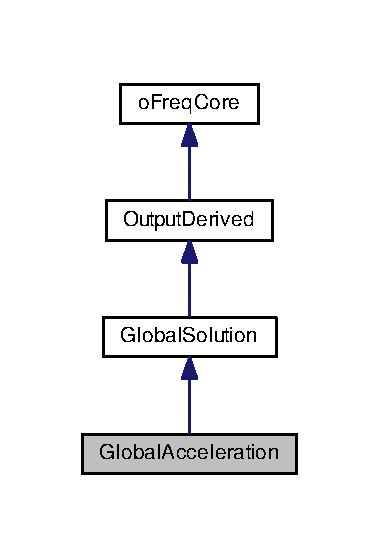
\includegraphics[width=182pt]{class_global_acceleration__inherit__graph}
\end{center}
\end{figure}


Collaboration diagram for Global\-Acceleration\-:
\nopagebreak
\begin{figure}[H]
\begin{center}
\leavevmode
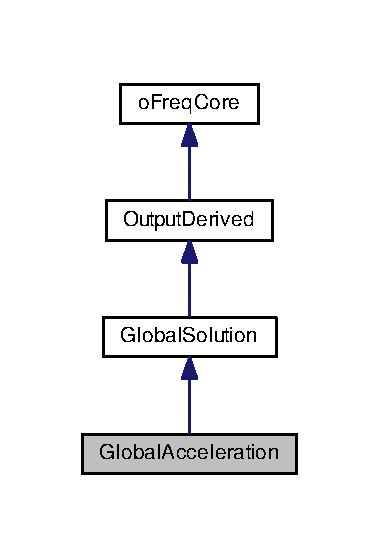
\includegraphics[width=182pt]{class_global_acceleration__coll__graph}
\end{center}
\end{figure}
\subsection*{Public Member Functions}
\begin{DoxyCompactItemize}
\item 
\hyperlink{class_global_acceleration_a37a05fcecd06641847388428a3f43fb8}{Global\-Acceleration} ()
\item 
\hyperlink{class_global_acceleration_aafb7853a1923f0e06b96f2ef4eca03d3}{$\sim$\-Global\-Acceleration} ()
\item 
void \hyperlink{class_global_acceleration_a14a041ea42d4c1bc10211c9a44aa3431}{set\-Derivative} (int ord)
\begin{DoxyCompactList}\small\item\em Sets the order of the derivative for the object. \end{DoxyCompactList}\end{DoxyCompactItemize}
\subsection*{Additional Inherited Members}


\subsection{Detailed Description}
This class represents the Global Acceleraion \hyperlink{class_solution}{Solution}. 

\subsection{Constructor \& Destructor Documentation}
\hypertarget{class_global_acceleration_a37a05fcecd06641847388428a3f43fb8}{\index{Global\-Acceleration@{Global\-Acceleration}!Global\-Acceleration@{Global\-Acceleration}}
\index{Global\-Acceleration@{Global\-Acceleration}!GlobalAcceleration@{Global\-Acceleration}}
\subsubsection[{Global\-Acceleration}]{\setlength{\rightskip}{0pt plus 5cm}Global\-Acceleration\-::\-Global\-Acceleration (
\begin{DoxyParamCaption}
{}
\end{DoxyParamCaption}
)}}\label{class_global_acceleration_a37a05fcecd06641847388428a3f43fb8}
This default constructor creates a Global Acceleration object. \hypertarget{class_global_acceleration_aafb7853a1923f0e06b96f2ef4eca03d3}{\index{Global\-Acceleration@{Global\-Acceleration}!$\sim$\-Global\-Acceleration@{$\sim$\-Global\-Acceleration}}
\index{$\sim$\-Global\-Acceleration@{$\sim$\-Global\-Acceleration}!GlobalAcceleration@{Global\-Acceleration}}
\subsubsection[{$\sim$\-Global\-Acceleration}]{\setlength{\rightskip}{0pt plus 5cm}Global\-Acceleration\-::$\sim$\-Global\-Acceleration (
\begin{DoxyParamCaption}
{}
\end{DoxyParamCaption}
)}}\label{class_global_acceleration_aafb7853a1923f0e06b96f2ef4eca03d3}
The default destructor, nothing happens here. 

\subsection{Member Function Documentation}
\hypertarget{class_global_acceleration_a14a041ea42d4c1bc10211c9a44aa3431}{\index{Global\-Acceleration@{Global\-Acceleration}!set\-Derivative@{set\-Derivative}}
\index{set\-Derivative@{set\-Derivative}!GlobalAcceleration@{Global\-Acceleration}}
\subsubsection[{set\-Derivative}]{\setlength{\rightskip}{0pt plus 5cm}void Global\-Acceleration\-::set\-Derivative (
\begin{DoxyParamCaption}
\item[{int}]{ord}
\end{DoxyParamCaption}
)\hspace{0.3cm}{\ttfamily [virtual]}}}\label{class_global_acceleration_a14a041ea42d4c1bc10211c9a44aa3431}


Sets the order of the derivative for the object. 


\begin{DoxyParams}{Parameters}
{\em ord} & Integer input that specifies the order of the derivative. Value can be anything from 0 or larger. Variable is passed by value. \\
\hline
\end{DoxyParams}


Reimplemented from \hyperlink{class_global_solution_a537163391f1f55d073720b20f69acfa5}{Global\-Solution}.



Here is the call graph for this function\-:\nopagebreak
\begin{figure}[H]
\begin{center}
\leavevmode
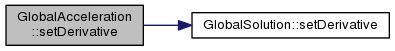
\includegraphics[width=350pt]{class_global_acceleration_a14a041ea42d4c1bc10211c9a44aa3431_cgraph}
\end{center}
\end{figure}




The documentation for this class was generated from the following files\-:\begin{DoxyCompactItemize}
\item 
globalacceleration.\-h\item 
globalacceleration.\-cpp\end{DoxyCompactItemize}

\hypertarget{class_global_motion}{\section{Global\-Motion Class Reference}
\label{class_global_motion}\index{Global\-Motion@{Global\-Motion}}
}


{\ttfamily \#include $<$globalmotion.\-h$>$}



Inheritance diagram for Global\-Motion\-:\nopagebreak
\begin{figure}[H]
\begin{center}
\leavevmode
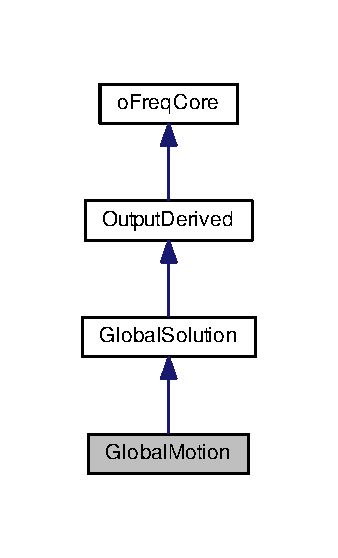
\includegraphics[width=162pt]{class_global_motion__inherit__graph}
\end{center}
\end{figure}


Collaboration diagram for Global\-Motion\-:\nopagebreak
\begin{figure}[H]
\begin{center}
\leavevmode
\includegraphics[width=162pt]{class_global_motion__coll__graph}
\end{center}
\end{figure}
\subsection*{Public Member Functions}
\begin{DoxyCompactItemize}
\item 
\hyperlink{class_global_motion_afe0b801895608782addf27d231bce572}{Global\-Motion} ()
\item 
\hyperlink{class_global_motion_aee21eade3de9cb666a6b8fa42cf1e9e1}{$\sim$\-Global\-Motion} ()
\item 
void \hyperlink{class_global_motion_a15a8c0d57ffedf65a1cd84154cdaa6ae}{set\-Derivative} (int ord)
\begin{DoxyCompactList}\small\item\em Sets the order of the derivative for the object. \end{DoxyCompactList}\end{DoxyCompactItemize}
\subsection*{Additional Inherited Members}


\subsection{Detailed Description}
This class represents the Global Motion \hyperlink{class_solution}{Solution}. 

\subsection{Constructor \& Destructor Documentation}
\hypertarget{class_global_motion_afe0b801895608782addf27d231bce572}{\index{Global\-Motion@{Global\-Motion}!Global\-Motion@{Global\-Motion}}
\index{Global\-Motion@{Global\-Motion}!GlobalMotion@{Global\-Motion}}
\subsubsection[{Global\-Motion}]{\setlength{\rightskip}{0pt plus 5cm}Global\-Motion\-::\-Global\-Motion (
\begin{DoxyParamCaption}
{}
\end{DoxyParamCaption}
)}}\label{class_global_motion_afe0b801895608782addf27d231bce572}
This default constructor creates a Global Motion object. \hypertarget{class_global_motion_aee21eade3de9cb666a6b8fa42cf1e9e1}{\index{Global\-Motion@{Global\-Motion}!$\sim$\-Global\-Motion@{$\sim$\-Global\-Motion}}
\index{$\sim$\-Global\-Motion@{$\sim$\-Global\-Motion}!GlobalMotion@{Global\-Motion}}
\subsubsection[{$\sim$\-Global\-Motion}]{\setlength{\rightskip}{0pt plus 5cm}Global\-Motion\-::$\sim$\-Global\-Motion (
\begin{DoxyParamCaption}
{}
\end{DoxyParamCaption}
)}}\label{class_global_motion_aee21eade3de9cb666a6b8fa42cf1e9e1}
The default destructor, nothing happens here. 

\subsection{Member Function Documentation}
\hypertarget{class_global_motion_a15a8c0d57ffedf65a1cd84154cdaa6ae}{\index{Global\-Motion@{Global\-Motion}!set\-Derivative@{set\-Derivative}}
\index{set\-Derivative@{set\-Derivative}!GlobalMotion@{Global\-Motion}}
\subsubsection[{set\-Derivative}]{\setlength{\rightskip}{0pt plus 5cm}void Global\-Motion\-::set\-Derivative (
\begin{DoxyParamCaption}
\item[{int}]{ord}
\end{DoxyParamCaption}
)\hspace{0.3cm}{\ttfamily [virtual]}}}\label{class_global_motion_a15a8c0d57ffedf65a1cd84154cdaa6ae}


Sets the order of the derivative for the object. 


\begin{DoxyParams}{Parameters}
{\em ord} & Integer input that specifies the order of the derivative. Value can be anything from 0 or larger. Variable is passed by value. \\
\hline
\end{DoxyParams}


Reimplemented from \hyperlink{class_global_solution_a537163391f1f55d073720b20f69acfa5}{Global\-Solution}.



Here is the call graph for this function\-:\nopagebreak
\begin{figure}[H]
\begin{center}
\leavevmode
\includegraphics[width=350pt]{class_global_motion_a15a8c0d57ffedf65a1cd84154cdaa6ae_cgraph}
\end{center}
\end{figure}




The documentation for this class was generated from the following files\-:\begin{DoxyCompactItemize}
\item 
/home/nicholas/\-Ship Design/\-Projects/\-D\-M\-S1305 Open\-S\-E\-A/master/200\-\_\-src/bin/ofreq/derived\-\_\-outputs/globalmotion.\-h\item 
/home/nicholas/\-Ship Design/\-Projects/\-D\-M\-S1305 Open\-S\-E\-A/master/200\-\_\-src/bin/ofreq/derived\-\_\-outputs/globalmotion.\-cpp\end{DoxyCompactItemize}

\hypertarget{class_global_solution}{\section{Global\-Solution Class Reference}
\label{class_global_solution}\index{Global\-Solution@{Global\-Solution}}
}


{\ttfamily \#include $<$globalsolution.\-h$>$}



Inheritance diagram for Global\-Solution\-:\nopagebreak
\begin{figure}[H]
\begin{center}
\leavevmode
\includegraphics[width=350pt]{class_global_solution__inherit__graph}
\end{center}
\end{figure}


Collaboration diagram for Global\-Solution\-:\nopagebreak
\begin{figure}[H]
\begin{center}
\leavevmode
\includegraphics[width=162pt]{class_global_solution__coll__graph}
\end{center}
\end{figure}
\subsection*{Public Member Functions}
\begin{DoxyCompactItemize}
\item 
\hyperlink{class_global_solution_a27fcfb056c30fc07f8937bc71ec677e6}{Global\-Solution} ()
\item 
\hyperlink{class_global_solution_aea630b237ced06e04c5ea00bf1bb9398}{$\sim$\-Global\-Solution} ()
\item 
virtual void \hyperlink{class_global_solution_a537163391f1f55d073720b20f69acfa5}{set\-Derivative} (int ord)
\begin{DoxyCompactList}\small\item\em Sets the order of the derivative for the object. \end{DoxyCompactList}\item 
int \hyperlink{class_global_solution_abf8fa956895f2728820d65fda2f5304d}{get\-Derivative} ()
\begin{DoxyCompactList}\small\item\em Gets the order of derivative set for the object. \end{DoxyCompactList}\item 
cx\-\_\-mat \hyperlink{class_global_solution_adf90922a97153ce858da530e20bc3f4d}{calc\-Output} (double freq\-In)
\begin{DoxyCompactList}\small\item\em Calculates the \hyperlink{class_global_solution}{Global\-Solution} output. \hyperlink{class_global_solution}{Global\-Solution} is the direct output of the solution for each body, translated into body coordinates. The output is modified to provide the specified order of derivative for the solution. \end{DoxyCompactList}\end{DoxyCompactItemize}
\subsection*{Protected Member Functions}
\begin{DoxyCompactItemize}
\item 
\hyperlink{class_solution}{Solution} \& \hyperlink{class_global_solution_a43a8caad9f88e3b468c3e9a364b45500}{get\-Solution} (double freq\-In)
\begin{DoxyCompactList}\small\item\em Gets the solution matrix to perform operations on. Accesses the solution matrix from the parent body. \end{DoxyCompactList}\end{DoxyCompactItemize}
\subsection*{Protected Attributes}
\begin{DoxyCompactItemize}
\item 
\hypertarget{class_global_solution_a026746ffb8e416eb4142a058b108148c}{int \hyperlink{class_global_solution_a026746ffb8e416eb4142a058b108148c}{order\-Derivative}}\label{class_global_solution_a026746ffb8e416eb4142a058b108148c}

\begin{DoxyCompactList}\small\item\em The order of derivative to use for calculating output. Set by child classes for specifying specific outputs. \end{DoxyCompactList}\end{DoxyCompactItemize}


\subsection{Detailed Description}
This class represents the Global \hyperlink{class_solution}{Solution}. The Global \hyperlink{class_solution}{Solution} is the direct output of the solved values for each body. It provides the motions calculated for each body, translated back to body coordinate system. The \hyperlink{class_global_solution}{Global\-Solution} can output any desired derivative of the solved motions. Several other child classes are derived from this class. The only difference is that for those other classes, the order of derivative is predefined. \begin{DoxySeeAlso}{See Also}
\hyperlink{class_global_motion}{Global\-Motion} 

\hyperlink{class_global_velocity}{Global\-Velocity} 

\hyperlink{class_global_acceleration}{Global\-Acceleration} 
\end{DoxySeeAlso}


\subsection{Constructor \& Destructor Documentation}
\hypertarget{class_global_solution_a27fcfb056c30fc07f8937bc71ec677e6}{\index{Global\-Solution@{Global\-Solution}!Global\-Solution@{Global\-Solution}}
\index{Global\-Solution@{Global\-Solution}!GlobalSolution@{Global\-Solution}}
\subsubsection[{Global\-Solution}]{\setlength{\rightskip}{0pt plus 5cm}Global\-Solution\-::\-Global\-Solution (
\begin{DoxyParamCaption}
{}
\end{DoxyParamCaption}
)}}\label{class_global_solution_a27fcfb056c30fc07f8937bc71ec677e6}
This default constructor creates a Global \hyperlink{class_solution}{Solution} object. 

Here is the call graph for this function\-:\nopagebreak
\begin{figure}[H]
\begin{center}
\leavevmode
\includegraphics[width=350pt]{class_global_solution_a27fcfb056c30fc07f8937bc71ec677e6_cgraph}
\end{center}
\end{figure}


\hypertarget{class_global_solution_aea630b237ced06e04c5ea00bf1bb9398}{\index{Global\-Solution@{Global\-Solution}!$\sim$\-Global\-Solution@{$\sim$\-Global\-Solution}}
\index{$\sim$\-Global\-Solution@{$\sim$\-Global\-Solution}!GlobalSolution@{Global\-Solution}}
\subsubsection[{$\sim$\-Global\-Solution}]{\setlength{\rightskip}{0pt plus 5cm}Global\-Solution\-::$\sim$\-Global\-Solution (
\begin{DoxyParamCaption}
{}
\end{DoxyParamCaption}
)}}\label{class_global_solution_aea630b237ced06e04c5ea00bf1bb9398}
The default destructor, nothing happens here. 

\subsection{Member Function Documentation}
\hypertarget{class_global_solution_adf90922a97153ce858da530e20bc3f4d}{\index{Global\-Solution@{Global\-Solution}!calc\-Output@{calc\-Output}}
\index{calc\-Output@{calc\-Output}!GlobalSolution@{Global\-Solution}}
\subsubsection[{calc\-Output}]{\setlength{\rightskip}{0pt plus 5cm}cx\-\_\-mat Global\-Solution\-::calc\-Output (
\begin{DoxyParamCaption}
\item[{double}]{freq\-In}
\end{DoxyParamCaption}
)\hspace{0.3cm}{\ttfamily [virtual]}}}\label{class_global_solution_adf90922a97153ce858da530e20bc3f4d}


Calculates the \hyperlink{class_global_solution}{Global\-Solution} output. \hyperlink{class_global_solution}{Global\-Solution} is the direct output of the solution for each body, translated into body coordinates. The output is modified to provide the specified order of derivative for the solution. 


\begin{DoxyParams}{Parameters}
{\em freq\-In} & The wave frequency to use for calculating the \hyperlink{class_output_derived}{Output\-Derived} object. Most outputs will depend on the wave frequency. \\
\hline
\end{DoxyParams}
\begin{DoxyReturn}{Returns}
Returns a complex matrix that is the \hyperlink{class_global_solution}{Global\-Solution} object. The complex matrix is a single row matrix. Each column in the row matrix represents a new degree of freedom variable. 
\end{DoxyReturn}


Implements \hyperlink{class_output_derived_a7a65864e45519edfe7fe45c408457f41}{Output\-Derived}.



Here is the call graph for this function\-:\nopagebreak
\begin{figure}[H]
\begin{center}
\leavevmode
\includegraphics[width=350pt]{class_global_solution_adf90922a97153ce858da530e20bc3f4d_cgraph}
\end{center}
\end{figure}


\hypertarget{class_global_solution_abf8fa956895f2728820d65fda2f5304d}{\index{Global\-Solution@{Global\-Solution}!get\-Derivative@{get\-Derivative}}
\index{get\-Derivative@{get\-Derivative}!GlobalSolution@{Global\-Solution}}
\subsubsection[{get\-Derivative}]{\setlength{\rightskip}{0pt plus 5cm}int Global\-Solution\-::get\-Derivative (
\begin{DoxyParamCaption}
{}
\end{DoxyParamCaption}
)}}\label{class_global_solution_abf8fa956895f2728820d65fda2f5304d}


Gets the order of derivative set for the object. 

\begin{DoxyReturn}{Returns}
Integer that specifies the order of the derivative. Value can be anything from 0 or larger. Variable is passed by value. 
\end{DoxyReturn}
\hypertarget{class_global_solution_a43a8caad9f88e3b468c3e9a364b45500}{\index{Global\-Solution@{Global\-Solution}!get\-Solution@{get\-Solution}}
\index{get\-Solution@{get\-Solution}!GlobalSolution@{Global\-Solution}}
\subsubsection[{get\-Solution}]{\setlength{\rightskip}{0pt plus 5cm}{\bf Solution} \& Global\-Solution\-::get\-Solution (
\begin{DoxyParamCaption}
\item[{double}]{freq\-In}
\end{DoxyParamCaption}
)\hspace{0.3cm}{\ttfamily [protected]}}}\label{class_global_solution_a43a8caad9f88e3b468c3e9a364b45500}


Gets the solution matrix to perform operations on. Accesses the solution matrix from the parent body. 


\begin{DoxyParams}{Parameters}
{\em freq\-In} & The wave frequency. Used to identify which variable to access in the solution matrix. \\
\hline
\end{DoxyParams}
\begin{DoxyReturn}{Returns}
Returns the \hyperlink{class_solution}{Solution} object to use for calculations. Variable is passed by reference. 
\end{DoxyReturn}


Here is the caller graph for this function\-:\nopagebreak
\begin{figure}[H]
\begin{center}
\leavevmode
\includegraphics[width=350pt]{class_global_solution_a43a8caad9f88e3b468c3e9a364b45500_icgraph}
\end{center}
\end{figure}


\hypertarget{class_global_solution_a537163391f1f55d073720b20f69acfa5}{\index{Global\-Solution@{Global\-Solution}!set\-Derivative@{set\-Derivative}}
\index{set\-Derivative@{set\-Derivative}!GlobalSolution@{Global\-Solution}}
\subsubsection[{set\-Derivative}]{\setlength{\rightskip}{0pt plus 5cm}void Global\-Solution\-::set\-Derivative (
\begin{DoxyParamCaption}
\item[{int}]{ord}
\end{DoxyParamCaption}
)\hspace{0.3cm}{\ttfamily [virtual]}}}\label{class_global_solution_a537163391f1f55d073720b20f69acfa5}


Sets the order of the derivative for the object. 


\begin{DoxyParams}{Parameters}
{\em ord} & Integer input that specifies the order of the derivative. Value can be anything from 0 or larger. Variable is passed by value. \\
\hline
\end{DoxyParams}


Reimplemented in \hyperlink{class_global_acceleration_a14a041ea42d4c1bc10211c9a44aa3431}{Global\-Acceleration}, \hyperlink{class_global_motion_a15a8c0d57ffedf65a1cd84154cdaa6ae}{Global\-Motion}, and \hyperlink{class_global_velocity_a11229a6dbc7f85f3c321b5eddb127f10}{Global\-Velocity}.



Here is the caller graph for this function\-:\nopagebreak
\begin{figure}[H]
\begin{center}
\leavevmode
\includegraphics[width=350pt]{class_global_solution_a537163391f1f55d073720b20f69acfa5_icgraph}
\end{center}
\end{figure}




The documentation for this class was generated from the following files\-:\begin{DoxyCompactItemize}
\item 
/home/nicholas/\-Ship Design/\-Projects/\-D\-M\-S1305 Open\-S\-E\-A/master/200\-\_\-src/bin/ofreq/derived\-\_\-outputs/globalsolution.\-h\item 
/home/nicholas/\-Ship Design/\-Projects/\-D\-M\-S1305 Open\-S\-E\-A/master/200\-\_\-src/bin/ofreq/derived\-\_\-outputs/globalsolution.\-cpp\end{DoxyCompactItemize}

\hypertarget{class_global_velocity}{\section{Global\-Velocity Class Reference}
\label{class_global_velocity}\index{Global\-Velocity@{Global\-Velocity}}
}


{\ttfamily \#include $<$globalvelocity.\-h$>$}



Inheritance diagram for Global\-Velocity\-:
\nopagebreak
\begin{figure}[H]
\begin{center}
\leavevmode
\includegraphics[width=162pt]{class_global_velocity__inherit__graph}
\end{center}
\end{figure}


Collaboration diagram for Global\-Velocity\-:
\nopagebreak
\begin{figure}[H]
\begin{center}
\leavevmode
\includegraphics[width=162pt]{class_global_velocity__coll__graph}
\end{center}
\end{figure}
\subsection*{Public Member Functions}
\begin{DoxyCompactItemize}
\item 
\hyperlink{class_global_velocity_a444ab39b351acd4e6ca7dc8088e2a9b8}{Global\-Velocity} ()
\item 
\hyperlink{class_global_velocity_a2b8f719180b1786a582d90603db8f2d8}{$\sim$\-Global\-Velocity} ()
\item 
\hypertarget{class_global_velocity_a11229a6dbc7f85f3c321b5eddb127f10}{void {\bfseries set\-Derivative} (int ord)}\label{class_global_velocity_a11229a6dbc7f85f3c321b5eddb127f10}

\end{DoxyCompactItemize}


\subsection{Detailed Description}
This class represents the Global Velocity \hyperlink{class_solution}{Solution}. 

\subsection{Constructor \& Destructor Documentation}
\hypertarget{class_global_velocity_a444ab39b351acd4e6ca7dc8088e2a9b8}{\index{Global\-Velocity@{Global\-Velocity}!Global\-Velocity@{Global\-Velocity}}
\index{Global\-Velocity@{Global\-Velocity}!GlobalVelocity@{Global\-Velocity}}
\subsubsection[{Global\-Velocity}]{\setlength{\rightskip}{0pt plus 5cm}Global\-Velocity\-::\-Global\-Velocity (
\begin{DoxyParamCaption}
{}
\end{DoxyParamCaption}
)}}\label{class_global_velocity_a444ab39b351acd4e6ca7dc8088e2a9b8}
This default constructor creates a Global Velocity object. \hypertarget{class_global_velocity_a2b8f719180b1786a582d90603db8f2d8}{\index{Global\-Velocity@{Global\-Velocity}!$\sim$\-Global\-Velocity@{$\sim$\-Global\-Velocity}}
\index{$\sim$\-Global\-Velocity@{$\sim$\-Global\-Velocity}!GlobalVelocity@{Global\-Velocity}}
\subsubsection[{$\sim$\-Global\-Velocity}]{\setlength{\rightskip}{0pt plus 5cm}Global\-Velocity\-::$\sim$\-Global\-Velocity (
\begin{DoxyParamCaption}
{}
\end{DoxyParamCaption}
)}}\label{class_global_velocity_a2b8f719180b1786a582d90603db8f2d8}
The default destructor, nothing happens here. 

The documentation for this class was generated from the following files\-:\begin{DoxyCompactItemize}
\item 
globalvelocity.\-h\item 
globalvelocity.\-cpp\end{DoxyCompactItemize}

\hypertarget{class_hydrodynamic_input}{\section{Hydrodynamic\-Input Class Reference}
\label{class_hydrodynamic_input}\index{Hydrodynamic\-Input@{Hydrodynamic\-Input}}
}


Inheritance diagram for Hydrodynamic\-Input\-:\nopagebreak
\begin{figure}[H]
\begin{center}
\leavevmode
\includegraphics[width=180pt]{class_hydrodynamic_input__inherit__graph}
\end{center}
\end{figure}


Collaboration diagram for Hydrodynamic\-Input\-:\nopagebreak
\begin{figure}[H]
\begin{center}
\leavevmode
\includegraphics[width=180pt]{class_hydrodynamic_input__coll__graph}
\end{center}
\end{figure}
\subsection*{Protected Member Functions}
\begin{DoxyCompactItemize}
\item 
void \hyperlink{class_hydrodynamic_input_a311ec06f62b7929fb6712e90240a1436}{initialize\-Defaults} ()
\item 
\hypertarget{class_hydrodynamic_input_a5497b513fc1785b84dccea59fd16fff2}{void {\bfseries set\-Data} (istream \&)}\label{class_hydrodynamic_input_a5497b513fc1785b84dccea59fd16fff2}

\item 
int \hyperlink{class_hydrodynamic_input_a6cf4ad1a8407191c8e2633ca0554f641}{legal\-Keyword} (string)
\end{DoxyCompactItemize}
\subsection*{Additional Inherited Members}


\subsection{Member Function Documentation}
\hypertarget{class_hydrodynamic_input_a311ec06f62b7929fb6712e90240a1436}{\index{Hydrodynamic\-Input@{Hydrodynamic\-Input}!initialize\-Defaults@{initialize\-Defaults}}
\index{initialize\-Defaults@{initialize\-Defaults}!HydrodynamicInput@{Hydrodynamic\-Input}}
\subsubsection[{initialize\-Defaults}]{\setlength{\rightskip}{0pt plus 5cm}void Hydrodynamic\-Input\-::initialize\-Defaults (
\begin{DoxyParamCaption}
{}
\end{DoxyParamCaption}
)\hspace{0.3cm}{\ttfamily [protected]}, {\ttfamily [virtual]}}}\label{class_hydrodynamic_input_a311ec06f62b7929fb6712e90240a1436}
Must be implemented by child class. 

Implements \hyperlink{class_read_input_a4ff2727b876cfd7c01299b08bdd65646}{Read\-Input}.

\hypertarget{class_hydrodynamic_input_a6cf4ad1a8407191c8e2633ca0554f641}{\index{Hydrodynamic\-Input@{Hydrodynamic\-Input}!legal\-Keyword@{legal\-Keyword}}
\index{legal\-Keyword@{legal\-Keyword}!HydrodynamicInput@{Hydrodynamic\-Input}}
\subsubsection[{legal\-Keyword}]{\setlength{\rightskip}{0pt plus 5cm}int Hydrodynamic\-Input\-::legal\-Keyword (
\begin{DoxyParamCaption}
\item[{string}]{}
\end{DoxyParamCaption}
)\hspace{0.3cm}{\ttfamily [protected]}, {\ttfamily [virtual]}}}\label{class_hydrodynamic_input_a6cf4ad1a8407191c8e2633ca0554f641}
Must be implemented by child class, determine if keyword is legal. 

Implements \hyperlink{class_read_input_a4c67f10e813686bf635dd4c6bb2c61bc}{Read\-Input}.



The documentation for this class was generated from the following files\-:\begin{DoxyCompactItemize}
\item 
/home/nicholas/\-Ship Design/\-Projects/\-D\-M\-S1305 Open\-S\-E\-A/master/200\-\_\-src/bin/ofreq/file\-\_\-reader/hydrodynamicinput.\-h\item 
/home/nicholas/\-Ship Design/\-Projects/\-D\-M\-S1305 Open\-S\-E\-A/master/200\-\_\-src/bin/ofreq/file\-\_\-reader/hydrodynamicinput.\-cpp\end{DoxyCompactItemize}

\hypertarget{class_motion_model}{\section{Motion\-Model Class Reference}
\label{class_motion_model}\index{Motion\-Model@{Motion\-Model}}
}


{\ttfamily \#include $<$motionmodel.\-h$>$}



Inheritance diagram for Motion\-Model\-:\nopagebreak
\begin{figure}[H]
\begin{center}
\leavevmode
\includegraphics[width=154pt]{class_motion_model__inherit__graph}
\end{center}
\end{figure}


Collaboration diagram for Motion\-Model\-:\nopagebreak
\begin{figure}[H]
\begin{center}
\leavevmode
\includegraphics[width=154pt]{class_motion_model__coll__graph}
\end{center}
\end{figure}
\subsection*{Public Member Functions}
\begin{DoxyCompactItemize}
\item 
\hyperlink{class_motion_model_a5a5e4bba0f6ca24e1fdd316458f4f824}{Motion\-Model} ()
\item 
\hyperlink{class_motion_model_a6a790fa8f769da8e97bae08e25b6fde8}{Motion\-Model} (vector$<$ \hyperlink{class_body}{Body} $>$ \&list\-Bod\-In)
\begin{DoxyCompactList}\small\item\em Constructor. This is the preferred constructor as it supplies the body data. \end{DoxyCompactList}\item 
\hyperlink{class_motion_model_ac48a359c77d9efe39d4ec8c9e862a1cd}{$\sim$\-Motion\-Model} ()
\item 
void \hyperlink{class_motion_model_a4a62fab7349a99d8f62a8693bffd92b5}{setlist\-Body} (vector$<$ \hyperlink{class_body}{Body} $>$ \&list\-Bod\-In)
\begin{DoxyCompactList}\small\item\em Inputs the list of body data. \end{DoxyCompactList}\item 
void \hyperlink{class_motion_model_a713b903a3e78141fff2af9c045755ffb}{set\-Body} (int bod)
\begin{DoxyCompactList}\small\item\em Sets the index for the body that all calculations are based on. \end{DoxyCompactList}\item 
bool \& \hyperlink{class_motion_model_af4d34bfa133e77f1527cee1aa36b02f4}{Coefficient\-Only} ()
\begin{DoxyCompactList}\small\item\em Determines whether the class should calculate force coefficients or actual force values. True = Calculate force coefficients only. False = Calculate force values. Default = (False) Calculate force values. \end{DoxyCompactList}\item 
bool \hyperlink{class_motion_model_afc54a14912e56315505ef5dbec28bd39}{get\-Active\-Only} ()
\begin{DoxyCompactList}\small\item\em Boolean to track whether only the active forces are requested. \end{DoxyCompactList}\item 
vector$<$ int $>$ \& \hyperlink{class_motion_model_ac4169ab37ab7d69f5030a0d67cb3dc86}{list\-Comp\-Cross\-Bod\-\_\-hydro} ()
\begin{DoxyCompactList}\small\item\em Records the index of the body object referenced by the cross body. \end{DoxyCompactList}\item 
int \& \hyperlink{class_motion_model_abe445279c6f964b5a64e046945249ea9}{list\-Comp\-Cross\-Bod\-\_\-hydro} (int crossbod\-In)
\begin{DoxyCompactList}\small\item\em Records the index of the body object referenced by the cross body. \end{DoxyCompactList}\item 
vector$<$ int $>$ \& \hyperlink{class_motion_model_a873a325f0017d73989cee1cdf8285b3c}{list\-Comp\-Cross\-Bod\-\_\-user} ()
\begin{DoxyCompactList}\small\item\em Records the index of the body object referenced by the cross body. \end{DoxyCompactList}\item 
int \& \hyperlink{class_motion_model_a63d9e54f8cbb434f67753fe737a89ee6}{list\-Comp\-Cross\-Bod\-\_\-user} (int crossbod\-In)
\begin{DoxyCompactList}\small\item\em Records the index of the body object referenced by the cross body. \end{DoxyCompactList}\item 
\hypertarget{class_motion_model_a27842d2b76ab078534c0626601da446b}{void \hyperlink{class_motion_model_a27842d2b76ab078534c0626601da446b}{Reset} ()}\label{class_motion_model_a27842d2b76ab078534c0626601da446b}

\begin{DoxyCompactList}\small\item\em Resets the class data to have all input coefficients. Any evaluation after a reset will produce a value of zero. \hyperlink{class_force}{Force} coefficients will be zero and force values will be zero. \end{DoxyCompactList}\item 
void \hyperlink{class_motion_model_a18e880b4a0b1a1d1c385bc3be3524440}{set\-Freq} (double freq)
\begin{DoxyCompactList}\small\item\em Sets the current operating frequency for the function. Only necessary when calculating true forces and using derivatives defined in the motion model. Otherwise, you can safely ignore this function. \end{DoxyCompactList}\item 
double \hyperlink{class_motion_model_a3461ede3739b468b6bab3a05f94093cc}{get\-Freq} ()
\begin{DoxyCompactList}\small\item\em Gets the current operating frequency for the function. Only necessary when calculating true forces and using derivatives defined in the motion model. Otherwise, you can safely ignore this function. \end{DoxyCompactList}\item 
void \hyperlink{class_motion_model_aaf761fac4693612a10771e38993431a0}{use\-Force\-Active\-\_\-user} (unsigned int force, unsigned int eqn)
\begin{DoxyCompactList}\small\item\em Passes information to the object to use input coefficients from the entry specified. \end{DoxyCompactList}\item 
void \hyperlink{class_motion_model_a4d3e0590135e1a9f7ce954406f99ff44}{use\-Force\-Active\-\_\-hydro} (unsigned int force, unsigned int eqn)
\begin{DoxyCompactList}\small\item\em Passes information to the object to use input coefficients from the entry specified. \end{DoxyCompactList}\item 
void \hyperlink{class_motion_model_a7db1d1ebebe216d17efd7b38f2e9deec}{use\-Force\-React\-\_\-user} (unsigned int force, unsigned int ord, unsigned int eqn, unsigned int var)
\begin{DoxyCompactList}\small\item\em Passes information to the object to use input coefficients from the entry specified. \end{DoxyCompactList}\item 
void \hyperlink{class_motion_model_ae3d2c7527ea2daddc6a85b6e02febb45}{use\-Force\-React\-\_\-hydro} (unsigned int force, unsigned int ord, unsigned int eqn, unsigned int var)
\begin{DoxyCompactList}\small\item\em Passes information to the object to use input coefficients from the entry specified. \end{DoxyCompactList}\item 
void \hyperlink{class_motion_model_a1159117995080d2b62e50fceaeb29778}{use\-Force\-Cross\-\_\-user} (unsigned int force, unsigned int ord, unsigned int eqn, unsigned int var)
\begin{DoxyCompactList}\small\item\em Passes information to the object to use input coefficients from the entry specified. \end{DoxyCompactList}\item 
void \hyperlink{class_motion_model_abfd6e4a22ec23d7ee462adb737fab3f2}{use\-Force\-Cross\-\_\-hydro} (unsigned int force, unsigned int ord, unsigned int eqn, unsigned int var)
\begin{DoxyCompactList}\small\item\em Passes information to the object to use input coefficients from the entry specified. \end{DoxyCompactList}\item 
void \hyperlink{class_motion_model_aecaf9f0261355cff2acf602acd728644}{use\-Force\-Mass} (unsigned int eqn, unsigned int var)
\begin{DoxyCompactList}\small\item\em Passes information to the object to use input coefficients from the entry specified. \end{DoxyCompactList}\item 
cx\-\_\-mat \hyperlink{class_motion_model_af9d30b6afa16093429fab496d18c5d00}{get\-Mat\-Force\-Active\-\_\-user} (int force)
\begin{DoxyCompactList}\small\item\em Evaluates the motion model for a whole range of equations on the specified force. \end{DoxyCompactList}\item 
cx\-\_\-mat \hyperlink{class_motion_model_a56059a3d7f37c9dad5f906714ba159de}{get\-Mat\-Force\-Active\-\_\-hydro} (int force)
\begin{DoxyCompactList}\small\item\em Evaluates the motion model for a whole range of equations on the specified force. \end{DoxyCompactList}\item 
cx\-\_\-mat \hyperlink{class_motion_model_a44e885c0255e74d82664c785499138f0}{get\-Mat\-Force\-React\-\_\-user} (int force, int ord)
\begin{DoxyCompactList}\small\item\em Evaluates the motion model for a whole range of equations and variable on the specified force and order of derivative. \end{DoxyCompactList}\item 
cx\-\_\-mat \hyperlink{class_motion_model_af239389973af6d198a21ee0c07db19c6}{get\-Mat\-Force\-React\-\_\-hydro} (int force, int ord)
\begin{DoxyCompactList}\small\item\em Evaluates the motion model for a whole range of equations and variable on the specified force and order of derivative. \end{DoxyCompactList}\item 
cx\-\_\-mat \hyperlink{class_motion_model_addbd875f2fc266823f645fc7f2d207e8}{get\-Mat\-Force\-Cross\-\_\-user} (int force, int ord)
\begin{DoxyCompactList}\small\item\em Evaluates the motion model for a whole range of equations and variable on the specified force and order of derivative. \end{DoxyCompactList}\item 
cx\-\_\-mat \hyperlink{class_motion_model_a7d661c296c3fe5c97322a62cceabb5d4}{get\-Mat\-Force\-Cross\-\_\-hydro} (int force, int ord)
\begin{DoxyCompactList}\small\item\em Evaluates the motion model for a whole range of equations and variable on the specified force and order of derivative. \end{DoxyCompactList}\item 
cx\-\_\-mat \hyperlink{class_motion_model_a7215db9f6f0c3e79f4559a4b9eadbcfc}{get\-Mat\-Force\-Mass} ()
\begin{DoxyCompactList}\small\item\em Evaluates the motion model for a whole range of equations and variable on the specified force and order of derivative. \end{DoxyCompactList}\item 
complex$<$ double $>$ \hyperlink{class_motion_model_a331d96a45df8ca0911fc4610705c3a30}{Evaluate} (int eqn)
\begin{DoxyCompactList}\small\item\em Triggers evaluation of the currently activated set of input coefficients. \end{DoxyCompactList}\item 
int \hyperlink{class_motion_model_a0a228c24a524e2a1c6636d3121a842be}{num\-Equations} ()
\begin{DoxyCompactList}\small\item\em Reports the number of equations used in the motion model. \end{DoxyCompactList}\item 
vector$<$ int $>$ \& \hyperlink{class_motion_model_ac62401cfe337e9404867819c529f2300}{ref\-Data\-Index} ()
\begin{DoxyCompactList}\small\item\em Returns a vector containing all equation indices. This may be the same as the number of equations. Very few equations may be used. However, if they are custom equations, they must avoid the first six indices, which are reserved for standard 6dof models. \end{DoxyCompactList}\item 
int \hyperlink{class_motion_model_a81ed21162a09ffce06043f3a7fb4213d}{Max\-Data\-Index} ()
\begin{DoxyCompactList}\small\item\em Returns the maximum number of the data index. \end{DoxyCompactList}\item 
void \hyperlink{class_motion_model_ad0da46b7982308fedcd87331f9d47d18}{set\-Name} (string name\-In)
\begin{DoxyCompactList}\small\item\em Name for the motion model. \end{DoxyCompactList}\item 
string \hyperlink{class_motion_model_af9fd1e58735b7f47bc5d5257bdca9139}{get\-Name} ()
\begin{DoxyCompactList}\small\item\em Name for the motion model. \end{DoxyCompactList}\item 
void \hyperlink{class_motion_model_a48cc314ff0f0c831c40bf1c399240b17}{set\-Description} (string Desc\-In)
\begin{DoxyCompactList}\small\item\em Description for the motion model. \end{DoxyCompactList}\item 
string \hyperlink{class_motion_model_a8594356137407b25d03927a68a422dc9}{get\-Description} ()
\begin{DoxyCompactList}\small\item\em Description for the motion model. \end{DoxyCompactList}\item 
vector$<$ \hyperlink{class_body}{Body} $>$ \& \hyperlink{class_motion_model_a67ad0e6b993a20af61170cdebe8f418f}{list\-Body} ()
\begin{DoxyCompactList}\small\item\em Provides direct access to the list of Bodies referenced by the motion model. \end{DoxyCompactList}\item 
\hyperlink{class_body}{Body} \& \hyperlink{class_motion_model_a3c08da3c6cb3e959b53f2cf6f614d3c0}{list\-Body} (int bod\-In)
\begin{DoxyCompactList}\small\item\em Direct access to an individual \hyperlink{class_body}{Body} from the list of Bodies contained in the motion model. \end{DoxyCompactList}\item 
vector$<$ \hyperlink{class_body}{Body} $>$ \& \hyperlink{class_motion_model_ae63712716bcaff9ff263d9728f39323a}{list\-Data} ()
\begin{DoxyCompactList}\small\item\em Provides direct access to the list of Bodies used as data for the motion model. \end{DoxyCompactList}\item 
\hyperlink{class_body}{Body} \& \hyperlink{class_motion_model_a1d7e2b929c15789259aaf732efd7f752}{list\-Data} (int data\-In)
\begin{DoxyCompactList}\small\item\em Direct access to an individual \hyperlink{class_body}{Body} from the list of Data contained in the motion model. \end{DoxyCompactList}\item 
vector$<$ \hyperlink{class_equationof_motion}{Equationof\-Motion} $>$ \& \hyperlink{class_motion_model_a608c356b5eb21fee5036a44124497815}{list\-Equation} ()
\begin{DoxyCompactList}\small\item\em Provides direct access to the list of equation of motion objects used in the motion model. \end{DoxyCompactList}\item 
\hyperlink{class_equationof_motion}{Equationof\-Motion} \& \hyperlink{class_motion_model_a444cd6e6ca1aea0822545b732118aeb9}{list\-Equation} (int eq\-In)
\begin{DoxyCompactList}\small\item\em Direct access to an individual \hyperlink{class_equationof_motion}{Equationof\-Motion} object from the list of Equations contained in the motion model. \end{DoxyCompactList}\end{DoxyCompactItemize}
\subsection*{Additional Inherited Members}


\subsection{Detailed Description}
This class provides the functionality to translate between input coefficients in the body class and the force coefficients in the \hyperlink{classmat_body}{mat\-Body} class. Most important, it acts as an interface for advanced users to enter their own equations of motion. This was devised to create a very generic interface that could allow any sort of definition for equations. The use of functions for the class should use the following sequence. 1.) Create class\-: constructor 2.) Set body data (if not already done in constructor)\-: set\-List\-Bodies 3.) Set the current body working with\-: set\-Body 4.) Set the current wave frequency working with\-: set\-Freq 5.) Set whether calculating coefficients or values (default\-: Values)\-: calc\-Coefficient 6.) Reset the forces you wish to use. 7.) Set the new list of forces you wish to use.\-: use\-Force\-Act\-\_\-usr use\-Force\-Act\-\_\-hydro use\-Force\-React\-\_\-usr use\-Force\-React\-\_\-hydro use\-Force\-Cross\-\_\-usr use\-Force\-Cross\-\_\-hydro use\-Force\-Mass 7.) Evaluate the motion model to produce a single complex value result. 

\subsection{Constructor \& Destructor Documentation}
\hypertarget{class_motion_model_a5a5e4bba0f6ca24e1fdd316458f4f824}{\index{Motion\-Model@{Motion\-Model}!Motion\-Model@{Motion\-Model}}
\index{Motion\-Model@{Motion\-Model}!MotionModel@{Motion\-Model}}
\subsubsection[{Motion\-Model}]{\setlength{\rightskip}{0pt plus 5cm}Motion\-Model\-::\-Motion\-Model (
\begin{DoxyParamCaption}
{}
\end{DoxyParamCaption}
)}}\label{class_motion_model_a5a5e4bba0f6ca24e1fdd316458f4f824}
Default constructor. \hypertarget{class_motion_model_a6a790fa8f769da8e97bae08e25b6fde8}{\index{Motion\-Model@{Motion\-Model}!Motion\-Model@{Motion\-Model}}
\index{Motion\-Model@{Motion\-Model}!MotionModel@{Motion\-Model}}
\subsubsection[{Motion\-Model}]{\setlength{\rightskip}{0pt plus 5cm}Motion\-Model\-::\-Motion\-Model (
\begin{DoxyParamCaption}
\item[{vector$<$ {\bf Body} $>$ \&}]{list\-Bod\-In}
\end{DoxyParamCaption}
)}}\label{class_motion_model_a6a790fa8f769da8e97bae08e25b6fde8}


Constructor. This is the preferred constructor as it supplies the body data. 


\begin{DoxyParams}{Parameters}
{\em list\-Bod\-In} & The vector of the body objects to input. \\
\hline
\end{DoxyParams}


Here is the call graph for this function\-:
\nopagebreak
\begin{figure}[H]
\begin{center}
\leavevmode
\includegraphics[width=350pt]{class_motion_model_a6a790fa8f769da8e97bae08e25b6fde8_cgraph}
\end{center}
\end{figure}


\hypertarget{class_motion_model_ac48a359c77d9efe39d4ec8c9e862a1cd}{\index{Motion\-Model@{Motion\-Model}!$\sim$\-Motion\-Model@{$\sim$\-Motion\-Model}}
\index{$\sim$\-Motion\-Model@{$\sim$\-Motion\-Model}!MotionModel@{Motion\-Model}}
\subsubsection[{$\sim$\-Motion\-Model}]{\setlength{\rightskip}{0pt plus 5cm}Motion\-Model\-::$\sim$\-Motion\-Model (
\begin{DoxyParamCaption}
{}
\end{DoxyParamCaption}
)}}\label{class_motion_model_ac48a359c77d9efe39d4ec8c9e862a1cd}
Default destructor. 

\subsection{Member Function Documentation}
\hypertarget{class_motion_model_af4d34bfa133e77f1527cee1aa36b02f4}{\index{Motion\-Model@{Motion\-Model}!Coefficient\-Only@{Coefficient\-Only}}
\index{Coefficient\-Only@{Coefficient\-Only}!MotionModel@{Motion\-Model}}
\subsubsection[{Coefficient\-Only}]{\setlength{\rightskip}{0pt plus 5cm}bool \& Motion\-Model\-::\-Coefficient\-Only (
\begin{DoxyParamCaption}
{}
\end{DoxyParamCaption}
)}}\label{class_motion_model_af4d34bfa133e77f1527cee1aa36b02f4}


Determines whether the class should calculate force coefficients or actual force values. True = Calculate force coefficients only. False = Calculate force values. Default = (False) Calculate force values. 

\begin{DoxyReturn}{Returns}
Boolean to determine whether should calculate coefficients or values. 
\end{DoxyReturn}


Here is the caller graph for this function\-:\nopagebreak
\begin{figure}[H]
\begin{center}
\leavevmode
\includegraphics[width=350pt]{class_motion_model_af4d34bfa133e77f1527cee1aa36b02f4_icgraph}
\end{center}
\end{figure}


\hypertarget{class_motion_model_a331d96a45df8ca0911fc4610705c3a30}{\index{Motion\-Model@{Motion\-Model}!Evaluate@{Evaluate}}
\index{Evaluate@{Evaluate}!MotionModel@{Motion\-Model}}
\subsubsection[{Evaluate}]{\setlength{\rightskip}{0pt plus 5cm}complex$<$ double $>$ Motion\-Model\-::\-Evaluate (
\begin{DoxyParamCaption}
\item[{int}]{eqn}
\end{DoxyParamCaption}
)}}\label{class_motion_model_a331d96a45df8ca0911fc4610705c3a30}


Triggers evaluation of the currently activated set of input coefficients. 

Triggers evaluation of the currently activated set of input coefficients. If Calc\-\_\-\-Coeff is set to True, then evaluation will only generate the force coefficients from the resulting evaluation. Otherwise, the evaluation will use the currently defined solution data and evaluate for force values. 
\begin{DoxyParams}{Parameters}
{\em eqn} & Integer representing which equation object to evaluate. \\
\hline
\end{DoxyParams}
\begin{DoxyReturn}{Returns}
Returns a complex number representing the force under the currently set conditions. 
\end{DoxyReturn}


Here is the caller graph for this function\-:\nopagebreak
\begin{figure}[H]
\begin{center}
\leavevmode
\includegraphics[width=350pt]{class_motion_model_a331d96a45df8ca0911fc4610705c3a30_icgraph}
\end{center}
\end{figure}


\hypertarget{class_motion_model_afc54a14912e56315505ef5dbec28bd39}{\index{Motion\-Model@{Motion\-Model}!get\-Active\-Only@{get\-Active\-Only}}
\index{get\-Active\-Only@{get\-Active\-Only}!MotionModel@{Motion\-Model}}
\subsubsection[{get\-Active\-Only}]{\setlength{\rightskip}{0pt plus 5cm}bool Motion\-Model\-::get\-Active\-Only (
\begin{DoxyParamCaption}
{}
\end{DoxyParamCaption}
)}}\label{class_motion_model_afc54a14912e56315505ef5dbec28bd39}


Boolean to track whether only the active forces are requested. 

Boolean to track whether only the active forces are requested. The active forces are included negatively in the equation of motion. They should be on the opposite side of the equation and included as a positive constant. The final matrix body accomplishes this. And when only active forces are requested, they should be sent out as positive values. However, when pulling the information out, the signs must be reversed. The boolean variable triggers to determine if this should happen. If any reactive or cross-\/body forces are activated as well, this variable is set false. \begin{DoxyReturn}{Returns}
Returns boolean variable. Variable passed by value. Returns true if only active forces are used in the equation of motion. Returns false if any reactive or cross-\/body forces are used in the equation of motion. 
\end{DoxyReturn}


Here is the caller graph for this function\-:\nopagebreak
\begin{figure}[H]
\begin{center}
\leavevmode
\includegraphics[width=350pt]{class_motion_model_afc54a14912e56315505ef5dbec28bd39_icgraph}
\end{center}
\end{figure}


\hypertarget{class_motion_model_a8594356137407b25d03927a68a422dc9}{\index{Motion\-Model@{Motion\-Model}!get\-Description@{get\-Description}}
\index{get\-Description@{get\-Description}!MotionModel@{Motion\-Model}}
\subsubsection[{get\-Description}]{\setlength{\rightskip}{0pt plus 5cm}string Motion\-Model\-::get\-Description (
\begin{DoxyParamCaption}
{}
\end{DoxyParamCaption}
)}}\label{class_motion_model_a8594356137407b25d03927a68a422dc9}


Description for the motion model. 

Description for the motion model. Used by the user to provide a more extensive description of the motion model. Used purely for user information. Not used for model identification. \begin{DoxyReturn}{Returns}
String. The description for the motion model. Variable passed by value. 
\end{DoxyReturn}
\hypertarget{class_motion_model_a3461ede3739b468b6bab3a05f94093cc}{\index{Motion\-Model@{Motion\-Model}!get\-Freq@{get\-Freq}}
\index{get\-Freq@{get\-Freq}!MotionModel@{Motion\-Model}}
\subsubsection[{get\-Freq}]{\setlength{\rightskip}{0pt plus 5cm}double Motion\-Model\-::get\-Freq (
\begin{DoxyParamCaption}
{}
\end{DoxyParamCaption}
)}}\label{class_motion_model_a3461ede3739b468b6bab3a05f94093cc}


Gets the current operating frequency for the function. Only necessary when calculating true forces and using derivatives defined in the motion model. Otherwise, you can safely ignore this function. 

\begin{DoxyReturn}{Returns}
Double precision variable that is the current wave frequency value. Variable returned by value. 
\end{DoxyReturn}


Here is the caller graph for this function\-:\nopagebreak
\begin{figure}[H]
\begin{center}
\leavevmode
\includegraphics[width=348pt]{class_motion_model_a3461ede3739b468b6bab3a05f94093cc_icgraph}
\end{center}
\end{figure}


\hypertarget{class_motion_model_a56059a3d7f37c9dad5f906714ba159de}{\index{Motion\-Model@{Motion\-Model}!get\-Mat\-Force\-Active\-\_\-hydro@{get\-Mat\-Force\-Active\-\_\-hydro}}
\index{get\-Mat\-Force\-Active\-\_\-hydro@{get\-Mat\-Force\-Active\-\_\-hydro}!MotionModel@{Motion\-Model}}
\subsubsection[{get\-Mat\-Force\-Active\-\_\-hydro}]{\setlength{\rightskip}{0pt plus 5cm}cx\-\_\-mat Motion\-Model\-::get\-Mat\-Force\-Active\-\_\-hydro (
\begin{DoxyParamCaption}
\item[{int}]{force}
\end{DoxyParamCaption}
)}}\label{class_motion_model_a56059a3d7f37c9dad5f906714ba159de}


Evaluates the motion model for a whole range of equations on the specified force. 

Evaluates the motion model for a whole range of equations on the specified force. Returns a complex matrix that contains the results of the entire evaluation. 
\begin{DoxyParams}{Parameters}
{\em force} & Integer specifying which force object to evaluate. \\
\hline
\end{DoxyParams}
\begin{DoxyReturn}{Returns}
Returns a complex matrix that contains the results of the entire evaluation. Returned argument passed by value. 
\end{DoxyReturn}


Here is the call graph for this function\-:
\nopagebreak
\begin{figure}[H]
\begin{center}
\leavevmode
\includegraphics[width=350pt]{class_motion_model_a56059a3d7f37c9dad5f906714ba159de_cgraph}
\end{center}
\end{figure}


\hypertarget{class_motion_model_af9d30b6afa16093429fab496d18c5d00}{\index{Motion\-Model@{Motion\-Model}!get\-Mat\-Force\-Active\-\_\-user@{get\-Mat\-Force\-Active\-\_\-user}}
\index{get\-Mat\-Force\-Active\-\_\-user@{get\-Mat\-Force\-Active\-\_\-user}!MotionModel@{Motion\-Model}}
\subsubsection[{get\-Mat\-Force\-Active\-\_\-user}]{\setlength{\rightskip}{0pt plus 5cm}cx\-\_\-mat Motion\-Model\-::get\-Mat\-Force\-Active\-\_\-user (
\begin{DoxyParamCaption}
\item[{int}]{force}
\end{DoxyParamCaption}
)}}\label{class_motion_model_af9d30b6afa16093429fab496d18c5d00}


Evaluates the motion model for a whole range of equations on the specified force. 

Evaluates the motion model for a whole range of equations on the specified force. Returns a complex matrix that contains the results of the entire evaluation. 
\begin{DoxyParams}{Parameters}
{\em force} & Integer specifying which force object to evaluate. \\
\hline
\end{DoxyParams}
\begin{DoxyReturn}{Returns}
Returns a complex matrix that contains the results of the entire evaluation. Returned argument passed by value. 
\end{DoxyReturn}


Here is the call graph for this function\-:
\nopagebreak
\begin{figure}[H]
\begin{center}
\leavevmode
\includegraphics[width=350pt]{class_motion_model_af9d30b6afa16093429fab496d18c5d00_cgraph}
\end{center}
\end{figure}


\hypertarget{class_motion_model_a7d661c296c3fe5c97322a62cceabb5d4}{\index{Motion\-Model@{Motion\-Model}!get\-Mat\-Force\-Cross\-\_\-hydro@{get\-Mat\-Force\-Cross\-\_\-hydro}}
\index{get\-Mat\-Force\-Cross\-\_\-hydro@{get\-Mat\-Force\-Cross\-\_\-hydro}!MotionModel@{Motion\-Model}}
\subsubsection[{get\-Mat\-Force\-Cross\-\_\-hydro}]{\setlength{\rightskip}{0pt plus 5cm}cx\-\_\-mat Motion\-Model\-::get\-Mat\-Force\-Cross\-\_\-hydro (
\begin{DoxyParamCaption}
\item[{int}]{force, }
\item[{int}]{ord}
\end{DoxyParamCaption}
)}}\label{class_motion_model_a7d661c296c3fe5c97322a62cceabb5d4}


Evaluates the motion model for a whole range of equations and variable on the specified force and order of derivative. 

Evaluates the motion model for a whole range of equations and variable on the specified force and order of derivative. Returns a complex matrix that contains the results of the entire evaluation. Saves some time on computing effort. 
\begin{DoxyParams}{Parameters}
{\em force} & Integer specifying the force object to use. \\
\hline
{\em ord} & Integer specifying which order of derivative to use on the specified force object. \\
\hline
\end{DoxyParams}
\begin{DoxyReturn}{Returns}
Returns a complex matrix that contains the results of the entire evaluation. Saves some time on computing effort. 
\end{DoxyReturn}


Here is the call graph for this function\-:
\nopagebreak
\begin{figure}[H]
\begin{center}
\leavevmode
\includegraphics[width=350pt]{class_motion_model_a7d661c296c3fe5c97322a62cceabb5d4_cgraph}
\end{center}
\end{figure}


\hypertarget{class_motion_model_addbd875f2fc266823f645fc7f2d207e8}{\index{Motion\-Model@{Motion\-Model}!get\-Mat\-Force\-Cross\-\_\-user@{get\-Mat\-Force\-Cross\-\_\-user}}
\index{get\-Mat\-Force\-Cross\-\_\-user@{get\-Mat\-Force\-Cross\-\_\-user}!MotionModel@{Motion\-Model}}
\subsubsection[{get\-Mat\-Force\-Cross\-\_\-user}]{\setlength{\rightskip}{0pt plus 5cm}cx\-\_\-mat Motion\-Model\-::get\-Mat\-Force\-Cross\-\_\-user (
\begin{DoxyParamCaption}
\item[{int}]{force, }
\item[{int}]{ord}
\end{DoxyParamCaption}
)}}\label{class_motion_model_addbd875f2fc266823f645fc7f2d207e8}


Evaluates the motion model for a whole range of equations and variable on the specified force and order of derivative. 

Evaluates the motion model for a whole range of equations and variable on the specified force and order of derivative. Returns a complex matrix that contains the results of the entire evaluation. Saves some time on computing effort. 
\begin{DoxyParams}{Parameters}
{\em force} & Integer specifying the force object to use. \\
\hline
{\em ord} & Integer specifying which order of derivative to use on the specified force object. \\
\hline
\end{DoxyParams}
\begin{DoxyReturn}{Returns}
Returns a complex matrix that contains the results of the entire evaluation. Saves some time on computing effort. 
\end{DoxyReturn}


Here is the call graph for this function\-:
\nopagebreak
\begin{figure}[H]
\begin{center}
\leavevmode
\includegraphics[width=350pt]{class_motion_model_addbd875f2fc266823f645fc7f2d207e8_cgraph}
\end{center}
\end{figure}


\hypertarget{class_motion_model_a7215db9f6f0c3e79f4559a4b9eadbcfc}{\index{Motion\-Model@{Motion\-Model}!get\-Mat\-Force\-Mass@{get\-Mat\-Force\-Mass}}
\index{get\-Mat\-Force\-Mass@{get\-Mat\-Force\-Mass}!MotionModel@{Motion\-Model}}
\subsubsection[{get\-Mat\-Force\-Mass}]{\setlength{\rightskip}{0pt plus 5cm}cx\-\_\-mat Motion\-Model\-::get\-Mat\-Force\-Mass (
\begin{DoxyParamCaption}
{}
\end{DoxyParamCaption}
)}}\label{class_motion_model_a7215db9f6f0c3e79f4559a4b9eadbcfc}


Evaluates the motion model for a whole range of equations and variable on the specified force and order of derivative. 

Evaluates the motion model for a whole range of equations and variable on the specified force and order of derivative. Returns a complex matrix that contains the results of the entire evaluation. Saves some time on computing effort. \begin{DoxyReturn}{Returns}
Returns a complex matrix that contains the results of the entire evaluation. Saves some time on computing effort. 
\end{DoxyReturn}


Here is the call graph for this function\-:\nopagebreak
\begin{figure}[H]
\begin{center}
\leavevmode
\includegraphics[width=350pt]{class_motion_model_a7215db9f6f0c3e79f4559a4b9eadbcfc_cgraph}
\end{center}
\end{figure}


\hypertarget{class_motion_model_af239389973af6d198a21ee0c07db19c6}{\index{Motion\-Model@{Motion\-Model}!get\-Mat\-Force\-React\-\_\-hydro@{get\-Mat\-Force\-React\-\_\-hydro}}
\index{get\-Mat\-Force\-React\-\_\-hydro@{get\-Mat\-Force\-React\-\_\-hydro}!MotionModel@{Motion\-Model}}
\subsubsection[{get\-Mat\-Force\-React\-\_\-hydro}]{\setlength{\rightskip}{0pt plus 5cm}cx\-\_\-mat Motion\-Model\-::get\-Mat\-Force\-React\-\_\-hydro (
\begin{DoxyParamCaption}
\item[{int}]{force, }
\item[{int}]{ord}
\end{DoxyParamCaption}
)}}\label{class_motion_model_af239389973af6d198a21ee0c07db19c6}


Evaluates the motion model for a whole range of equations and variable on the specified force and order of derivative. 

Evaluates the motion model for a whole range of equations and variable on the specified force and order of derivative. Returns a complex matrix that contains the results of the entire evaluation. Saves some time on computing effort. 
\begin{DoxyParams}{Parameters}
{\em force} & Integer specifying the force object to use. \\
\hline
{\em ord} & Integer specifying which order of derivative to use on the specified force object. \\
\hline
\end{DoxyParams}
\begin{DoxyReturn}{Returns}
Returns a complex matrix that contains the results of the entire evaluation. Saves some time on computing effort. 
\end{DoxyReturn}


Here is the call graph for this function\-:
\nopagebreak
\begin{figure}[H]
\begin{center}
\leavevmode
\includegraphics[width=350pt]{class_motion_model_af239389973af6d198a21ee0c07db19c6_cgraph}
\end{center}
\end{figure}


\hypertarget{class_motion_model_a44e885c0255e74d82664c785499138f0}{\index{Motion\-Model@{Motion\-Model}!get\-Mat\-Force\-React\-\_\-user@{get\-Mat\-Force\-React\-\_\-user}}
\index{get\-Mat\-Force\-React\-\_\-user@{get\-Mat\-Force\-React\-\_\-user}!MotionModel@{Motion\-Model}}
\subsubsection[{get\-Mat\-Force\-React\-\_\-user}]{\setlength{\rightskip}{0pt plus 5cm}cx\-\_\-mat Motion\-Model\-::get\-Mat\-Force\-React\-\_\-user (
\begin{DoxyParamCaption}
\item[{int}]{force, }
\item[{int}]{ord}
\end{DoxyParamCaption}
)}}\label{class_motion_model_a44e885c0255e74d82664c785499138f0}


Evaluates the motion model for a whole range of equations and variable on the specified force and order of derivative. 

Evaluates the motion model for a whole range of equations and variable on the specified force and order of derivative. Returns a complex matrix that contains the results of the entire evaluation. Saves some time on computing effort. 
\begin{DoxyParams}{Parameters}
{\em force} & Integer specifying the force object to use. \\
\hline
{\em ord} & Integer specifying which order of derivative to use on the specified force object. \\
\hline
\end{DoxyParams}
\begin{DoxyReturn}{Returns}
Returns a complex matrix that contains the results of the entire evaluation. Saves some time on computing effort. 
\end{DoxyReturn}


Here is the call graph for this function\-:
\nopagebreak
\begin{figure}[H]
\begin{center}
\leavevmode
\includegraphics[width=350pt]{class_motion_model_a44e885c0255e74d82664c785499138f0_cgraph}
\end{center}
\end{figure}


\hypertarget{class_motion_model_af9fd1e58735b7f47bc5d5257bdca9139}{\index{Motion\-Model@{Motion\-Model}!get\-Name@{get\-Name}}
\index{get\-Name@{get\-Name}!MotionModel@{Motion\-Model}}
\subsubsection[{get\-Name}]{\setlength{\rightskip}{0pt plus 5cm}string Motion\-Model\-::get\-Name (
\begin{DoxyParamCaption}
{}
\end{DoxyParamCaption}
)}}\label{class_motion_model_af9fd1e58735b7f47bc5d5257bdca9139}


Name for the motion model. 

Name for the motion model. Used by the user to identify the motion model. \begin{DoxyReturn}{Returns}
The name to set for the motion model. String variable. Variable passed by value. 
\end{DoxyReturn}
\hypertarget{class_motion_model_a67ad0e6b993a20af61170cdebe8f418f}{\index{Motion\-Model@{Motion\-Model}!list\-Body@{list\-Body}}
\index{list\-Body@{list\-Body}!MotionModel@{Motion\-Model}}
\subsubsection[{list\-Body}]{\setlength{\rightskip}{0pt plus 5cm}vector$<$ {\bf Body} $>$ \& Motion\-Model\-::list\-Body (
\begin{DoxyParamCaption}
{}
\end{DoxyParamCaption}
)}}\label{class_motion_model_a67ad0e6b993a20af61170cdebe8f418f}


Provides direct access to the list of Bodies referenced by the motion model. 

\begin{DoxyReturn}{Returns}
Reference to vector of \hyperlink{class_body}{Body} objects. Variable passed by reference. 
\end{DoxyReturn}
\begin{DoxySeeAlso}{See Also}
\hyperlink{class_body}{Body} 
\end{DoxySeeAlso}
\hypertarget{class_motion_model_a3c08da3c6cb3e959b53f2cf6f614d3c0}{\index{Motion\-Model@{Motion\-Model}!list\-Body@{list\-Body}}
\index{list\-Body@{list\-Body}!MotionModel@{Motion\-Model}}
\subsubsection[{list\-Body}]{\setlength{\rightskip}{0pt plus 5cm}{\bf Body} \& Motion\-Model\-::list\-Body (
\begin{DoxyParamCaption}
\item[{int}]{bod\-In}
\end{DoxyParamCaption}
)}}\label{class_motion_model_a3c08da3c6cb3e959b53f2cf6f614d3c0}


Direct access to an individual \hyperlink{class_body}{Body} from the list of Bodies contained in the motion model. 


\begin{DoxyParams}{Parameters}
{\em bod\-In} & Integer specifying which \hyperlink{class_body}{Body} object to access in the list of Bodies. \\
\hline
\end{DoxyParams}
\begin{DoxyReturn}{Returns}
Returns reference to the \hyperlink{class_body}{Body} object specified by input bod\-In. 
\end{DoxyReturn}
\begin{DoxySeeAlso}{See Also}
\hyperlink{class_motion_model_a67ad0e6b993a20af61170cdebe8f418f}{list\-Body()} 
\end{DoxySeeAlso}
\hypertarget{class_motion_model_ac4169ab37ab7d69f5030a0d67cb3dc86}{\index{Motion\-Model@{Motion\-Model}!list\-Comp\-Cross\-Bod\-\_\-hydro@{list\-Comp\-Cross\-Bod\-\_\-hydro}}
\index{list\-Comp\-Cross\-Bod\-\_\-hydro@{list\-Comp\-Cross\-Bod\-\_\-hydro}!MotionModel@{Motion\-Model}}
\subsubsection[{list\-Comp\-Cross\-Bod\-\_\-hydro}]{\setlength{\rightskip}{0pt plus 5cm}vector$<$ int $>$ \& Motion\-Model\-::list\-Comp\-Cross\-Bod\-\_\-hydro (
\begin{DoxyParamCaption}
{}
\end{DoxyParamCaption}
)}}\label{class_motion_model_ac4169ab37ab7d69f5030a0d67cb3dc86}


Records the index of the body object referenced by the cross body. 

Records the index of the body object referenced by the cross body. Each body object contains a list of pointers for the cross-\/body objects. Each cross-\/body force has a pointer associated with it. This pointer points to another body object. This allows comparison between memory addresses of different body objects. However, when the body objects are copied over, the pointers are now pointing to different, invalid memory addresses. to eliminate this problem in the motion model, the model will record the position of the body object in the vector of body objects. This forms a vector. Each entry in the vector represents one cross-\/body force for the current body. The integer entry in the vector is the integer index of the body that the cross-\/body force is linked to. \begin{DoxyReturn}{Returns}
Returns a vector of integers. Returned variable is passed by reference. Each entry in the vector represents one cross-\/body force for the current body. The integer entry in the vector is the integer index of the body that the cross-\/body force is linked to. 
\end{DoxyReturn}


Here is the caller graph for this function\-:\nopagebreak
\begin{figure}[H]
\begin{center}
\leavevmode
\includegraphics[width=350pt]{class_motion_model_ac4169ab37ab7d69f5030a0d67cb3dc86_icgraph}
\end{center}
\end{figure}


\hypertarget{class_motion_model_abe445279c6f964b5a64e046945249ea9}{\index{Motion\-Model@{Motion\-Model}!list\-Comp\-Cross\-Bod\-\_\-hydro@{list\-Comp\-Cross\-Bod\-\_\-hydro}}
\index{list\-Comp\-Cross\-Bod\-\_\-hydro@{list\-Comp\-Cross\-Bod\-\_\-hydro}!MotionModel@{Motion\-Model}}
\subsubsection[{list\-Comp\-Cross\-Bod\-\_\-hydro}]{\setlength{\rightskip}{0pt plus 5cm}int \& Motion\-Model\-::list\-Comp\-Cross\-Bod\-\_\-hydro (
\begin{DoxyParamCaption}
\item[{int}]{crossbod\-In}
\end{DoxyParamCaption}
)}}\label{class_motion_model_abe445279c6f964b5a64e046945249ea9}


Records the index of the body object referenced by the cross body. 

Records the index of the body object referenced by the cross body. Each body object contains a list of pointers for the cross-\/body objects. Each cross-\/body force has a pointer associated with it. This pointer points to another body object. This allows comparison between memory addresses of different body objects. However, when the body objects are copied over, the pointers are now pointing to different, invalid memory addresses. to eliminate this problem in the motion model, the model will record the position of the body object in the vector of body objects. This forms a vector. Each entry in the vector represents one cross-\/body force for the current body. The integer entry in the vector is the integer index of the body that the cross-\/body force is linked to. 
\begin{DoxyParams}{Parameters}
{\em crossbod\-In} & Integer parameter. Specified the index of which value to retrieve from the list of values for the Cross\-Bod indices. \\
\hline
\end{DoxyParams}
\begin{DoxyReturn}{Returns}
Returns an integer. Variable passed by reference. Returned integer is the index of the \hyperlink{class_body}{Body} object referenced by the cross-\/body force located at the index specified by Cross\-Bod. Example\-: Cross\-Bod (index) -\/$>$ (vector of cross body forces) -\/$>$ Index of \hyperlink{class_body}{Body} object that cross-\/body force points to. 
\end{DoxyReturn}
\hypertarget{class_motion_model_a873a325f0017d73989cee1cdf8285b3c}{\index{Motion\-Model@{Motion\-Model}!list\-Comp\-Cross\-Bod\-\_\-user@{list\-Comp\-Cross\-Bod\-\_\-user}}
\index{list\-Comp\-Cross\-Bod\-\_\-user@{list\-Comp\-Cross\-Bod\-\_\-user}!MotionModel@{Motion\-Model}}
\subsubsection[{list\-Comp\-Cross\-Bod\-\_\-user}]{\setlength{\rightskip}{0pt plus 5cm}vector$<$ int $>$ \& Motion\-Model\-::list\-Comp\-Cross\-Bod\-\_\-user (
\begin{DoxyParamCaption}
{}
\end{DoxyParamCaption}
)}}\label{class_motion_model_a873a325f0017d73989cee1cdf8285b3c}


Records the index of the body object referenced by the cross body. 

Records the index of the body object referenced by the cross body. Each body object contains a list of pointers for the cross-\/body objects. Each cross-\/body force has a pointer associated with it. This pointer points to another body object. This allows comparison between memory addresses of different body objects. However, when the body objects are copied over, the pointers are now pointing to different, invalid memory addresses. to eliminate this problem in the motion model, the model will record the position of the body object in the vector of body objects. This forms a vector. Each entry in the vector represents one cross-\/body force for the current body. The integer entry in the vector is the integer index of the body that the cross-\/body force is linked to. \begin{DoxyReturn}{Returns}
Returns a vector of integers. Returned variable is passed by reference. Each entry in the vector represents one cross-\/body force for the current body. The integer entry in the vector is the integer index of the body that the cross-\/body force is linked to. 
\end{DoxyReturn}


Here is the caller graph for this function\-:\nopagebreak
\begin{figure}[H]
\begin{center}
\leavevmode
\includegraphics[width=350pt]{class_motion_model_a873a325f0017d73989cee1cdf8285b3c_icgraph}
\end{center}
\end{figure}


\hypertarget{class_motion_model_a63d9e54f8cbb434f67753fe737a89ee6}{\index{Motion\-Model@{Motion\-Model}!list\-Comp\-Cross\-Bod\-\_\-user@{list\-Comp\-Cross\-Bod\-\_\-user}}
\index{list\-Comp\-Cross\-Bod\-\_\-user@{list\-Comp\-Cross\-Bod\-\_\-user}!MotionModel@{Motion\-Model}}
\subsubsection[{list\-Comp\-Cross\-Bod\-\_\-user}]{\setlength{\rightskip}{0pt plus 5cm}int \& Motion\-Model\-::list\-Comp\-Cross\-Bod\-\_\-user (
\begin{DoxyParamCaption}
\item[{int}]{crossbod\-In}
\end{DoxyParamCaption}
)}}\label{class_motion_model_a63d9e54f8cbb434f67753fe737a89ee6}


Records the index of the body object referenced by the cross body. 

Records the index of the body object referenced by the cross body. Each body object contains a list of pointers for the cross-\/body objects. Each cross-\/body force has a pointer associated with it. This pointer points to another body object. This allows comparison between memory addresses of different body objects. However, when the body objects are copied over, the pointers are now pointing to different, invalid memory addresses. to eliminate this problem in the motion model, the model will record the position of the body object in the vector of body objects. This forms a vector. Each entry in the vector represents one cross-\/body force for the current body. The integer entry in the vector is the integer index of the body that the cross-\/body force is linked to. 
\begin{DoxyParams}{Parameters}
{\em crossbod\-In} & Integer parameter. Specified the index of which value to retrieve from the list of values for the Cross\-Bod indices. \\
\hline
\end{DoxyParams}
\begin{DoxyReturn}{Returns}
Returns an integer. Variable passed by reference. Returned integer is the index of the \hyperlink{class_body}{Body} object referenced by the cross-\/body force located at the index specified by Cross\-Bod. Example\-: Cross\-Bod (index) -\/$>$ (vector of cross body forces) -\/$>$ Index of \hyperlink{class_body}{Body} object that cross-\/body force points to. 
\end{DoxyReturn}
\hypertarget{class_motion_model_ae63712716bcaff9ff263d9728f39323a}{\index{Motion\-Model@{Motion\-Model}!list\-Data@{list\-Data}}
\index{list\-Data@{list\-Data}!MotionModel@{Motion\-Model}}
\subsubsection[{list\-Data}]{\setlength{\rightskip}{0pt plus 5cm}vector$<$ {\bf Body} $>$ \& Motion\-Model\-::list\-Data (
\begin{DoxyParamCaption}
{}
\end{DoxyParamCaption}
)}}\label{class_motion_model_ae63712716bcaff9ff263d9728f39323a}


Provides direct access to the list of Bodies used as data for the motion model. 

\begin{DoxyReturn}{Returns}
Reference to the vector of \hyperlink{class_body}{Body} objects used as data. Variable passed by reference. 
\end{DoxyReturn}
\begin{DoxySeeAlso}{See Also}
\hyperlink{class_body}{Body} 
\end{DoxySeeAlso}


Here is the caller graph for this function\-:
\nopagebreak
\begin{figure}[H]
\begin{center}
\leavevmode
\includegraphics[width=350pt]{class_motion_model_ae63712716bcaff9ff263d9728f39323a_icgraph}
\end{center}
\end{figure}


\hypertarget{class_motion_model_a1d7e2b929c15789259aaf732efd7f752}{\index{Motion\-Model@{Motion\-Model}!list\-Data@{list\-Data}}
\index{list\-Data@{list\-Data}!MotionModel@{Motion\-Model}}
\subsubsection[{list\-Data}]{\setlength{\rightskip}{0pt plus 5cm}{\bf Body} \& Motion\-Model\-::list\-Data (
\begin{DoxyParamCaption}
\item[{int}]{data\-In}
\end{DoxyParamCaption}
)}}\label{class_motion_model_a1d7e2b929c15789259aaf732efd7f752}


Direct access to an individual \hyperlink{class_body}{Body} from the list of Data contained in the motion model. 


\begin{DoxyParams}{Parameters}
{\em data\-In} & Integer specifying which \hyperlink{class_body}{Body} object to access from the list of Data. \\
\hline
\end{DoxyParams}
\begin{DoxyReturn}{Returns}
Returns reference to the \hyperlink{class_body}{Body} object specified by data\-In. 
\end{DoxyReturn}
\begin{DoxySeeAlso}{See Also}
\hyperlink{class_motion_model_ae63712716bcaff9ff263d9728f39323a}{list\-Data()} 
\end{DoxySeeAlso}
\hypertarget{class_motion_model_a608c356b5eb21fee5036a44124497815}{\index{Motion\-Model@{Motion\-Model}!list\-Equation@{list\-Equation}}
\index{list\-Equation@{list\-Equation}!MotionModel@{Motion\-Model}}
\subsubsection[{list\-Equation}]{\setlength{\rightskip}{0pt plus 5cm}vector$<$ {\bf Equationof\-Motion} $>$ \& Motion\-Model\-::list\-Equation (
\begin{DoxyParamCaption}
{}
\end{DoxyParamCaption}
)}}\label{class_motion_model_a608c356b5eb21fee5036a44124497815}


Provides direct access to the list of equation of motion objects used in the motion model. 

\begin{DoxyReturn}{Returns}
Reference to the vector of \hyperlink{class_equationof_motion}{Equationof\-Motion} objects. Variable passed by reference. 
\end{DoxyReturn}
\begin{DoxySeeAlso}{See Also}
\hyperlink{class_equationof_motion}{Equationof\-Motion} 
\end{DoxySeeAlso}


Here is the caller graph for this function\-:
\nopagebreak
\begin{figure}[H]
\begin{center}
\leavevmode
\includegraphics[width=350pt]{class_motion_model_a608c356b5eb21fee5036a44124497815_icgraph}
\end{center}
\end{figure}


\hypertarget{class_motion_model_a444cd6e6ca1aea0822545b732118aeb9}{\index{Motion\-Model@{Motion\-Model}!list\-Equation@{list\-Equation}}
\index{list\-Equation@{list\-Equation}!MotionModel@{Motion\-Model}}
\subsubsection[{list\-Equation}]{\setlength{\rightskip}{0pt plus 5cm}{\bf Equationof\-Motion} \& Motion\-Model\-::list\-Equation (
\begin{DoxyParamCaption}
\item[{int}]{eq\-In}
\end{DoxyParamCaption}
)}}\label{class_motion_model_a444cd6e6ca1aea0822545b732118aeb9}


Direct access to an individual \hyperlink{class_equationof_motion}{Equationof\-Motion} object from the list of Equations contained in the motion model. 


\begin{DoxyParams}{Parameters}
{\em eq\-In} & Integer specifying which \hyperlink{class_equationof_motion}{Equationof\-Motion} object to access from the list of Equations \\
\hline
\end{DoxyParams}
\begin{DoxyReturn}{Returns}
Returns reference to the \hyperlink{class_equationof_motion}{Equationof\-Motion} object specified by eq\-In. 
\end{DoxyReturn}
\hypertarget{class_motion_model_a81ed21162a09ffce06043f3a7fb4213d}{\index{Motion\-Model@{Motion\-Model}!Max\-Data\-Index@{Max\-Data\-Index}}
\index{Max\-Data\-Index@{Max\-Data\-Index}!MotionModel@{Motion\-Model}}
\subsubsection[{Max\-Data\-Index}]{\setlength{\rightskip}{0pt plus 5cm}int Motion\-Model\-::\-Max\-Data\-Index (
\begin{DoxyParamCaption}
{}
\end{DoxyParamCaption}
)}}\label{class_motion_model_a81ed21162a09ffce06043f3a7fb4213d}


Returns the maximum number of the data index. 

Returns the maximum number of the data index. This may be the same as the number of equations. Very few equations may be used. However, if they are custom equations, they must avoid the first six indices, which are reserved for standard 6dof models. \begin{DoxyReturn}{Returns}
Returns integer number representing the maximum number of the data index found from all equations. 
\end{DoxyReturn}


Here is the call graph for this function\-:\nopagebreak
\begin{figure}[H]
\begin{center}
\leavevmode
\includegraphics[width=350pt]{class_motion_model_a81ed21162a09ffce06043f3a7fb4213d_cgraph}
\end{center}
\end{figure}


\hypertarget{class_motion_model_a0a228c24a524e2a1c6636d3121a842be}{\index{Motion\-Model@{Motion\-Model}!num\-Equations@{num\-Equations}}
\index{num\-Equations@{num\-Equations}!MotionModel@{Motion\-Model}}
\subsubsection[{num\-Equations}]{\setlength{\rightskip}{0pt plus 5cm}int Motion\-Model\-::num\-Equations (
\begin{DoxyParamCaption}
{}
\end{DoxyParamCaption}
)}}\label{class_motion_model_a0a228c24a524e2a1c6636d3121a842be}


Reports the number of equations used in the motion model. 

Reports the number of equations used in the motion model. This lets the \hyperlink{classmat_body}{mat\-Body} object know how many equations to prepare for. \begin{DoxyReturn}{Returns}
Returns the number of equations used in the motion model. 
\end{DoxyReturn}


Here is the caller graph for this function\-:\nopagebreak
\begin{figure}[H]
\begin{center}
\leavevmode
\includegraphics[width=350pt]{class_motion_model_a0a228c24a524e2a1c6636d3121a842be_icgraph}
\end{center}
\end{figure}


\hypertarget{class_motion_model_ac62401cfe337e9404867819c529f2300}{\index{Motion\-Model@{Motion\-Model}!ref\-Data\-Index@{ref\-Data\-Index}}
\index{ref\-Data\-Index@{ref\-Data\-Index}!MotionModel@{Motion\-Model}}
\subsubsection[{ref\-Data\-Index}]{\setlength{\rightskip}{0pt plus 5cm}vector$<$ int $>$ \& Motion\-Model\-::ref\-Data\-Index (
\begin{DoxyParamCaption}
{}
\end{DoxyParamCaption}
)}}\label{class_motion_model_ac62401cfe337e9404867819c529f2300}


Returns a vector containing all equation indices. This may be the same as the number of equations. Very few equations may be used. However, if they are custom equations, they must avoid the first six indices, which are reserved for standard 6dof models. 

\begin{DoxyReturn}{Returns}
Returns the highest count of the equation index. 
\end{DoxyReturn}


Here is the call graph for this function\-:\nopagebreak
\begin{figure}[H]
\begin{center}
\leavevmode
\includegraphics[width=350pt]{class_motion_model_ac62401cfe337e9404867819c529f2300_cgraph}
\end{center}
\end{figure}




Here is the caller graph for this function\-:\nopagebreak
\begin{figure}[H]
\begin{center}
\leavevmode
\includegraphics[width=350pt]{class_motion_model_ac62401cfe337e9404867819c529f2300_icgraph}
\end{center}
\end{figure}


\hypertarget{class_motion_model_a713b903a3e78141fff2af9c045755ffb}{\index{Motion\-Model@{Motion\-Model}!set\-Body@{set\-Body}}
\index{set\-Body@{set\-Body}!MotionModel@{Motion\-Model}}
\subsubsection[{set\-Body}]{\setlength{\rightskip}{0pt plus 5cm}void Motion\-Model\-::set\-Body (
\begin{DoxyParamCaption}
\item[{int}]{bod}
\end{DoxyParamCaption}
)}}\label{class_motion_model_a713b903a3e78141fff2af9c045755ffb}


Sets the index for the body that all calculations are based on. 


\begin{DoxyParams}{Parameters}
{\em Integer} & input specifying the number of the body to use. Integer corresponds to the sequence of bodies in the vector supplied with the body. \\
\hline
\end{DoxyParams}
\hypertarget{class_motion_model_a48cc314ff0f0c831c40bf1c399240b17}{\index{Motion\-Model@{Motion\-Model}!set\-Description@{set\-Description}}
\index{set\-Description@{set\-Description}!MotionModel@{Motion\-Model}}
\subsubsection[{set\-Description}]{\setlength{\rightskip}{0pt plus 5cm}void Motion\-Model\-::set\-Description (
\begin{DoxyParamCaption}
\item[{string}]{Desc\-In}
\end{DoxyParamCaption}
)}}\label{class_motion_model_a48cc314ff0f0c831c40bf1c399240b17}


Description for the motion model. 

Description for the motion model. Used by the user to provide a more extensive description of the motion model. Used purely for user information. Not used for model identification. 
\begin{DoxyParams}{Parameters}
{\em Desc\-In} & String. The description for the motion model. Variable passed by value. \\
\hline
\end{DoxyParams}
\hypertarget{class_motion_model_a18e880b4a0b1a1d1c385bc3be3524440}{\index{Motion\-Model@{Motion\-Model}!set\-Freq@{set\-Freq}}
\index{set\-Freq@{set\-Freq}!MotionModel@{Motion\-Model}}
\subsubsection[{set\-Freq}]{\setlength{\rightskip}{0pt plus 5cm}void Motion\-Model\-::set\-Freq (
\begin{DoxyParamCaption}
\item[{double}]{freq}
\end{DoxyParamCaption}
)}}\label{class_motion_model_a18e880b4a0b1a1d1c385bc3be3524440}


Sets the current operating frequency for the function. Only necessary when calculating true forces and using derivatives defined in the motion model. Otherwise, you can safely ignore this function. 


\begin{DoxyParams}{Parameters}
{\em Double} & precision value that sets the current wave frequency value. \\
\hline
\end{DoxyParams}
\hypertarget{class_motion_model_a4a62fab7349a99d8f62a8693bffd92b5}{\index{Motion\-Model@{Motion\-Model}!setlist\-Body@{setlist\-Body}}
\index{setlist\-Body@{setlist\-Body}!MotionModel@{Motion\-Model}}
\subsubsection[{setlist\-Body}]{\setlength{\rightskip}{0pt plus 5cm}void Motion\-Model\-::setlist\-Body (
\begin{DoxyParamCaption}
\item[{vector$<$ {\bf Body} $>$ \&}]{list\-Bod\-In}
\end{DoxyParamCaption}
)}}\label{class_motion_model_a4a62fab7349a99d8f62a8693bffd92b5}


Inputs the list of body data. 


\begin{DoxyParams}{Parameters}
{\em list\-Bod\-In} & The vector of body objects to input. \\
\hline
\end{DoxyParams}


Here is the caller graph for this function\-:
\nopagebreak
\begin{figure}[H]
\begin{center}
\leavevmode
\includegraphics[width=350pt]{class_motion_model_a4a62fab7349a99d8f62a8693bffd92b5_icgraph}
\end{center}
\end{figure}


\hypertarget{class_motion_model_ad0da46b7982308fedcd87331f9d47d18}{\index{Motion\-Model@{Motion\-Model}!set\-Name@{set\-Name}}
\index{set\-Name@{set\-Name}!MotionModel@{Motion\-Model}}
\subsubsection[{set\-Name}]{\setlength{\rightskip}{0pt plus 5cm}void Motion\-Model\-::set\-Name (
\begin{DoxyParamCaption}
\item[{string}]{name\-In}
\end{DoxyParamCaption}
)}}\label{class_motion_model_ad0da46b7982308fedcd87331f9d47d18}


Name for the motion model. 

Name for the motion model. Used by the user to identify the motion model. 
\begin{DoxyParams}{Parameters}
{\em name\-In} & The name to set for the motion model. String variable. Variable passed by value. \\
\hline
\end{DoxyParams}
\hypertarget{class_motion_model_a4d3e0590135e1a9f7ce954406f99ff44}{\index{Motion\-Model@{Motion\-Model}!use\-Force\-Active\-\_\-hydro@{use\-Force\-Active\-\_\-hydro}}
\index{use\-Force\-Active\-\_\-hydro@{use\-Force\-Active\-\_\-hydro}!MotionModel@{Motion\-Model}}
\subsubsection[{use\-Force\-Active\-\_\-hydro}]{\setlength{\rightskip}{0pt plus 5cm}void Motion\-Model\-::use\-Force\-Active\-\_\-hydro (
\begin{DoxyParamCaption}
\item[{unsigned int}]{force, }
\item[{unsigned int}]{eqn}
\end{DoxyParamCaption}
)}}\label{class_motion_model_a4d3e0590135e1a9f7ce954406f99ff44}


Passes information to the object to use input coefficients from the entry specified. 

Passes information to the object to use input coefficients from the entry specified. Limits inputs to only the force object type specified by the method. Calls to use\-Force methods are cumulative. Sucessive calls to different entries in the same force sequence will add their coefficients to the sets for evaluation. Can be combined with other use\-Force methods. Multiple calls to the same use\-Force method with the same index coordinates are not cumulative. An input coefficient can either be on or off, not multiple instances of the exact same coefficient. 
\begin{DoxyParams}{Parameters}
{\em force} & Integer specifying which force to use in the set of forces for the given force type. \\
\hline
{\em eqn} & Integer specifying which equation to use in the selected force. \\
\hline
\end{DoxyParams}


Here is the call graph for this function\-:
\nopagebreak
\begin{figure}[H]
\begin{center}
\leavevmode
\includegraphics[width=350pt]{class_motion_model_a4d3e0590135e1a9f7ce954406f99ff44_cgraph}
\end{center}
\end{figure}




Here is the caller graph for this function\-:\nopagebreak
\begin{figure}[H]
\begin{center}
\leavevmode
\includegraphics[width=350pt]{class_motion_model_a4d3e0590135e1a9f7ce954406f99ff44_icgraph}
\end{center}
\end{figure}


\hypertarget{class_motion_model_aaf761fac4693612a10771e38993431a0}{\index{Motion\-Model@{Motion\-Model}!use\-Force\-Active\-\_\-user@{use\-Force\-Active\-\_\-user}}
\index{use\-Force\-Active\-\_\-user@{use\-Force\-Active\-\_\-user}!MotionModel@{Motion\-Model}}
\subsubsection[{use\-Force\-Active\-\_\-user}]{\setlength{\rightskip}{0pt plus 5cm}void Motion\-Model\-::use\-Force\-Active\-\_\-user (
\begin{DoxyParamCaption}
\item[{unsigned int}]{force, }
\item[{unsigned int}]{eqn}
\end{DoxyParamCaption}
)}}\label{class_motion_model_aaf761fac4693612a10771e38993431a0}


Passes information to the object to use input coefficients from the entry specified. 

Passes information to the object to use input coefficients from the entry specified. Limits inputs to only the force object type specified by the method. Calls to use\-Force methods are cumulative. Sucessive calls to different entries in the same force sequence will add their coefficients to the sets for evaluation. Can be combined with other use\-Force methods. Multiple calls to the same use\-Force method with the same index coordinates are not cumulative. An input coefficient can either be on or off, not multiple instances of the exact same coefficient. 
\begin{DoxyParams}{Parameters}
{\em force} & Integer specifying which force to use in the set of forces for the given force type. \\
\hline
{\em eqn} & Integer specifying which equation to use in the selected force. \\
\hline
\end{DoxyParams}


Here is the call graph for this function\-:
\nopagebreak
\begin{figure}[H]
\begin{center}
\leavevmode
\includegraphics[width=350pt]{class_motion_model_aaf761fac4693612a10771e38993431a0_cgraph}
\end{center}
\end{figure}




Here is the caller graph for this function\-:\nopagebreak
\begin{figure}[H]
\begin{center}
\leavevmode
\includegraphics[width=350pt]{class_motion_model_aaf761fac4693612a10771e38993431a0_icgraph}
\end{center}
\end{figure}


\hypertarget{class_motion_model_abfd6e4a22ec23d7ee462adb737fab3f2}{\index{Motion\-Model@{Motion\-Model}!use\-Force\-Cross\-\_\-hydro@{use\-Force\-Cross\-\_\-hydro}}
\index{use\-Force\-Cross\-\_\-hydro@{use\-Force\-Cross\-\_\-hydro}!MotionModel@{Motion\-Model}}
\subsubsection[{use\-Force\-Cross\-\_\-hydro}]{\setlength{\rightskip}{0pt plus 5cm}void Motion\-Model\-::use\-Force\-Cross\-\_\-hydro (
\begin{DoxyParamCaption}
\item[{unsigned int}]{force, }
\item[{unsigned int}]{ord, }
\item[{unsigned int}]{eqn, }
\item[{unsigned int}]{var}
\end{DoxyParamCaption}
)}}\label{class_motion_model_abfd6e4a22ec23d7ee462adb737fab3f2}


Passes information to the object to use input coefficients from the entry specified. 

Passes information to the object to use input coefficients from the entry specified. Limits inputs to only the force object type specified by the method. Calls to use\-Force methods are cumulative. Sucessive calls to different entries in the same force sequence will add their coefficients to the sets for evaluation. Can be combined with other use\-Force methods. Multiple calls to the same use\-Force method with the same index coordinates are not cumulative. An input coefficient can either be on or off, not multiple instances of the exact same coefficient. 
\begin{DoxyParams}{Parameters}
{\em force} & Integer specifying which force to use in the set of forces for the given force type. \\
\hline
{\em ord} & Integer specifying which order of derviative to use for the selected force. \\
\hline
{\em eqn} & Integer specifying which equation to use in the selected force. \\
\hline
{\em var} & Integer specifying which variable to use from the selected equation. \\
\hline
\end{DoxyParams}


Here is the call graph for this function\-:
\nopagebreak
\begin{figure}[H]
\begin{center}
\leavevmode
\includegraphics[width=350pt]{class_motion_model_abfd6e4a22ec23d7ee462adb737fab3f2_cgraph}
\end{center}
\end{figure}




Here is the caller graph for this function\-:\nopagebreak
\begin{figure}[H]
\begin{center}
\leavevmode
\includegraphics[width=350pt]{class_motion_model_abfd6e4a22ec23d7ee462adb737fab3f2_icgraph}
\end{center}
\end{figure}


\hypertarget{class_motion_model_a1159117995080d2b62e50fceaeb29778}{\index{Motion\-Model@{Motion\-Model}!use\-Force\-Cross\-\_\-user@{use\-Force\-Cross\-\_\-user}}
\index{use\-Force\-Cross\-\_\-user@{use\-Force\-Cross\-\_\-user}!MotionModel@{Motion\-Model}}
\subsubsection[{use\-Force\-Cross\-\_\-user}]{\setlength{\rightskip}{0pt plus 5cm}void Motion\-Model\-::use\-Force\-Cross\-\_\-user (
\begin{DoxyParamCaption}
\item[{unsigned int}]{force, }
\item[{unsigned int}]{ord, }
\item[{unsigned int}]{eqn, }
\item[{unsigned int}]{var}
\end{DoxyParamCaption}
)}}\label{class_motion_model_a1159117995080d2b62e50fceaeb29778}


Passes information to the object to use input coefficients from the entry specified. 

Passes information to the object to use input coefficients from the entry specified. Limits inputs to only the force object type specified by the method. Calls to use\-Force methods are cumulative. Sucessive calls to different entries in the same force sequence will add their coefficients to the sets for evaluation. Can be combined with other use\-Force methods. Multiple calls to the same use\-Force method with the same index coordinates are not cumulative. An input coefficient can either be on or off, not multiple instances of the exact same coefficient. 
\begin{DoxyParams}{Parameters}
{\em force} & Integer specifying which force to use in the set of forces for the given force type. \\
\hline
{\em ord} & Integer specifying which order of derviative to use for the selected force. \\
\hline
{\em eqn} & Integer specifying which equation to use in the selected force. \\
\hline
{\em var} & Integer specifying which variable to use from the selected equation. \\
\hline
\end{DoxyParams}


Here is the call graph for this function\-:
\nopagebreak
\begin{figure}[H]
\begin{center}
\leavevmode
\includegraphics[width=350pt]{class_motion_model_a1159117995080d2b62e50fceaeb29778_cgraph}
\end{center}
\end{figure}




Here is the caller graph for this function\-:\nopagebreak
\begin{figure}[H]
\begin{center}
\leavevmode
\includegraphics[width=350pt]{class_motion_model_a1159117995080d2b62e50fceaeb29778_icgraph}
\end{center}
\end{figure}


\hypertarget{class_motion_model_aecaf9f0261355cff2acf602acd728644}{\index{Motion\-Model@{Motion\-Model}!use\-Force\-Mass@{use\-Force\-Mass}}
\index{use\-Force\-Mass@{use\-Force\-Mass}!MotionModel@{Motion\-Model}}
\subsubsection[{use\-Force\-Mass}]{\setlength{\rightskip}{0pt plus 5cm}void Motion\-Model\-::use\-Force\-Mass (
\begin{DoxyParamCaption}
\item[{unsigned int}]{eqn, }
\item[{unsigned int}]{var}
\end{DoxyParamCaption}
)}}\label{class_motion_model_aecaf9f0261355cff2acf602acd728644}


Passes information to the object to use input coefficients from the entry specified. 

Passes information to the object to use input coefficients from the entry specified. Limits inputs to only the force object type specified by the method. Calls to use\-Force methods are cumulative. Sucessive calls to different entries in the same force sequence will add their coefficients to the sets for evaluation. Can be combined with other use\-Force methods. Multiple calls to the same use\-Force method with the same index coordinates are not cumulative. An input coefficient can either be on or off, not multiple instances of the exact same coefficient. 
\begin{DoxyParams}{Parameters}
{\em eqn} & Integer specifying which equation to use in the selected force. \\
\hline
{\em var} & Integer specifying which variable to use from the selected equation. \\
\hline
\end{DoxyParams}


Here is the caller graph for this function\-:\nopagebreak
\begin{figure}[H]
\begin{center}
\leavevmode
\includegraphics[width=350pt]{class_motion_model_aecaf9f0261355cff2acf602acd728644_icgraph}
\end{center}
\end{figure}


\hypertarget{class_motion_model_ae3d2c7527ea2daddc6a85b6e02febb45}{\index{Motion\-Model@{Motion\-Model}!use\-Force\-React\-\_\-hydro@{use\-Force\-React\-\_\-hydro}}
\index{use\-Force\-React\-\_\-hydro@{use\-Force\-React\-\_\-hydro}!MotionModel@{Motion\-Model}}
\subsubsection[{use\-Force\-React\-\_\-hydro}]{\setlength{\rightskip}{0pt plus 5cm}void Motion\-Model\-::use\-Force\-React\-\_\-hydro (
\begin{DoxyParamCaption}
\item[{unsigned int}]{force, }
\item[{unsigned int}]{ord, }
\item[{unsigned int}]{eqn, }
\item[{unsigned int}]{var}
\end{DoxyParamCaption}
)}}\label{class_motion_model_ae3d2c7527ea2daddc6a85b6e02febb45}


Passes information to the object to use input coefficients from the entry specified. 

Passes information to the object to use input coefficients from the entry specified. Limits inputs to only the force object type specified by the method. Calls to use\-Force methods are cumulative. Sucessive calls to different entries in the same force sequence will add their coefficients to the sets for evaluation. Can be combined with other use\-Force methods. Multiple calls to the same use\-Force method with the same index coordinates are not cumulative. An input coefficient can either be on or off, not multiple instances of the exact same coefficient. 
\begin{DoxyParams}{Parameters}
{\em force} & Integer specifying which force to use in the set of forces for the given force type. \\
\hline
{\em ord} & Integer specifying which order of derviative to use for the selected force. \\
\hline
{\em eqn} & Integer specifying which equation to use in the selected force. \\
\hline
{\em var} & Integer specifying which variable to use from the selected equation. \\
\hline
\end{DoxyParams}


Here is the call graph for this function\-:
\nopagebreak
\begin{figure}[H]
\begin{center}
\leavevmode
\includegraphics[width=350pt]{class_motion_model_ae3d2c7527ea2daddc6a85b6e02febb45_cgraph}
\end{center}
\end{figure}




Here is the caller graph for this function\-:\nopagebreak
\begin{figure}[H]
\begin{center}
\leavevmode
\includegraphics[width=350pt]{class_motion_model_ae3d2c7527ea2daddc6a85b6e02febb45_icgraph}
\end{center}
\end{figure}


\hypertarget{class_motion_model_a7db1d1ebebe216d17efd7b38f2e9deec}{\index{Motion\-Model@{Motion\-Model}!use\-Force\-React\-\_\-user@{use\-Force\-React\-\_\-user}}
\index{use\-Force\-React\-\_\-user@{use\-Force\-React\-\_\-user}!MotionModel@{Motion\-Model}}
\subsubsection[{use\-Force\-React\-\_\-user}]{\setlength{\rightskip}{0pt plus 5cm}void Motion\-Model\-::use\-Force\-React\-\_\-user (
\begin{DoxyParamCaption}
\item[{unsigned int}]{force, }
\item[{unsigned int}]{ord, }
\item[{unsigned int}]{eqn, }
\item[{unsigned int}]{var}
\end{DoxyParamCaption}
)}}\label{class_motion_model_a7db1d1ebebe216d17efd7b38f2e9deec}


Passes information to the object to use input coefficients from the entry specified. 

Passes information to the object to use input coefficients from the entry specified. Limits inputs to only the force object type specified by the method. Calls to use\-Force methods are cumulative. Sucessive calls to different entries in the same force sequence will add their coefficients to the sets for evaluation. Can be combined with other use\-Force methods. Multiple calls to the same use\-Force method with the same index coordinates are not cumulative. An input coefficient can either be on or off, not multiple instances of the exact same coefficient. 
\begin{DoxyParams}{Parameters}
{\em force} & Integer specifying which force to use in the set of forces for the given force type. \\
\hline
{\em ord} & Integer specifying which order of derviative to use for the selected force. \\
\hline
{\em eqn} & Integer specifying which equation to use in the selected force. \\
\hline
{\em var} & Integer specifying which variable to use from the selected equation. \\
\hline
\end{DoxyParams}


Here is the call graph for this function\-:
\nopagebreak
\begin{figure}[H]
\begin{center}
\leavevmode
\includegraphics[width=350pt]{class_motion_model_a7db1d1ebebe216d17efd7b38f2e9deec_cgraph}
\end{center}
\end{figure}




Here is the caller graph for this function\-:\nopagebreak
\begin{figure}[H]
\begin{center}
\leavevmode
\includegraphics[width=350pt]{class_motion_model_a7db1d1ebebe216d17efd7b38f2e9deec_icgraph}
\end{center}
\end{figure}




The documentation for this class was generated from the following files\-:\begin{DoxyCompactItemize}
\item 
motionmodel.\-h\item 
motionmodel.\-cpp\end{DoxyCompactItemize}

\hypertarget{class_motion_solver}{\section{Motion\-Solver Class Reference}
\label{class_motion_solver}\index{Motion\-Solver@{Motion\-Solver}}
}


{\ttfamily \#include $<$motionsolver.\-h$>$}

\subsection*{Public Member Functions}
\begin{DoxyCompactItemize}
\item 
\hyperlink{class_motion_solver_ae231d7c407ef35357e519053091b6003}{Motion\-Solver} (vector$<$ \hyperlink{class_body}{Body} $>$, \hyperlink{class_user_forces}{User\-Forces}, double)
\item 
\hyperlink{class_motion_solver_ae1fb5f389752a21a6d65ce41599b9b91}{$\sim$\-Motion\-Solver} ()
\item 
void \hyperlink{class_motion_solver_ac6c03c2a45d7868b5acb76324fa29279}{set\-Matrix\-Index\-Positions} (int, int)
\item 
vector$<$ cx\-\_\-mat $>$ \hyperlink{class_motion_solver_a89c37a28a333474de2d0d51bada81afa}{sum\-Reactive\-Force\-Each\-Set} (vector$<$ \hyperlink{class_reactive_force_matrix}{Reactive\-Force\-Matrix} $>$)
\item 
cx\-\_\-mat \hyperlink{class_motion_solver_a58ec4344deda599d9b1de11aa3e6abde}{sum\-Active\-Force\-Each\-Set} (vector$<$ cx\-\_\-mat $>$)
\item 
cx\-\_\-mat \hyperlink{class_motion_solver_a26a41ac6907d24228de0a6ddcf9911ce}{sum\-Derivatives} (vector$<$ cx\-\_\-mat $>$)
\item 
vector$<$ cx\-\_\-mat $>$ \hyperlink{class_motion_solver_a2358d623842d0634576d978db98b9198}{Calculate\-Outputs} ()
\end{DoxyCompactItemize}
\subsection*{Public Attributes}
\begin{DoxyCompactItemize}
\item 
vector$<$ \hyperlink{class_body}{Body} $>$ \hyperlink{class_motion_solver_aa706c345b20614a18e9f8f59c6174d2a}{the\-Body\-Data}
\item 
\hyperlink{class_user_forces}{User\-Forces} \hyperlink{class_motion_solver_a9c8dd3a151361ae664c9ff4e9958f649}{the\-Forces\-Data}
\item 
vector$<$ \hyperlink{class_body_with_force_matrix}{Body\-With\-Force\-Matrix} $>$ \hyperlink{class_motion_solver_ac6c73cbeb23091b0064a9a2d0cd0752c}{the\-Body\-With\-Force\-Matrix}
\item 
\hyperlink{class_motion_model}{Motion\-Model} \hyperlink{class_motion_solver_a19e40f754e74afd9f99a3944360165bf}{the\-Motion\-Model}
\item 
double \hyperlink{class_motion_solver_a01ca22785130c0612045094790e2f992}{cur\-Wave\-Frequency}
\item 
int \hyperlink{class_motion_solver_af209f386af69a39839061e436630906c}{max\-Matrix\-Size}
\item 
cx\-\_\-mat \hyperlink{class_motion_solver_a29bb1f9a2fd145b4e8fc74ad711e4351}{reactive\-Force\-Matrix\-Global}
\item 
cx\-\_\-mat \hyperlink{class_motion_solver_a800bc918ff0075782368046bd51eeb87}{active\-Force\-Matrix\-Global}
\item 
cx\-\_\-mat \hyperlink{class_motion_solver_aba617c457e3dab115693c4b3a23f9827}{solution\-Column\-Matrix}
\end{DoxyCompactItemize}


\subsection{Detailed Description}
This class holds data for the motion solver and performs calculations on all of the data to get the solution matrix. 

\subsection{Constructor \& Destructor Documentation}
\hypertarget{class_motion_solver_ae231d7c407ef35357e519053091b6003}{\index{Motion\-Solver@{Motion\-Solver}!Motion\-Solver@{Motion\-Solver}}
\index{Motion\-Solver@{Motion\-Solver}!MotionSolver@{Motion\-Solver}}
\subsubsection[{Motion\-Solver}]{\setlength{\rightskip}{0pt plus 5cm}Motion\-Solver\-::\-Motion\-Solver (
\begin{DoxyParamCaption}
\item[{vector$<$ {\bf Body} $>$}]{body\-Data\-In, }
\item[{{\bf User\-Forces}}]{user\-Forces\-In, }
\item[{double}]{new\-Wave\-Freq}
\end{DoxyParamCaption}
)}}\label{class_motion_solver_ae231d7c407ef35357e519053091b6003}
The constructor. 
\begin{DoxyParams}{Parameters}
{\em body\-Data\-In} & The body. \\
\hline
{\em user\-Forces\-In} & The User Forces. \\
\hline
{\em new\-Wave\-Freq} & The wave frequencies. \\
\hline
\end{DoxyParams}
\hypertarget{class_motion_solver_ae1fb5f389752a21a6d65ce41599b9b91}{\index{Motion\-Solver@{Motion\-Solver}!$\sim$\-Motion\-Solver@{$\sim$\-Motion\-Solver}}
\index{$\sim$\-Motion\-Solver@{$\sim$\-Motion\-Solver}!MotionSolver@{Motion\-Solver}}
\subsubsection[{$\sim$\-Motion\-Solver}]{\setlength{\rightskip}{0pt plus 5cm}Motion\-Solver\-::$\sim$\-Motion\-Solver (
\begin{DoxyParamCaption}
{}
\end{DoxyParamCaption}
)}}\label{class_motion_solver_ae1fb5f389752a21a6d65ce41599b9b91}
The default destructor, nothing happens here. 

\subsection{Member Function Documentation}
\hypertarget{class_motion_solver_a2358d623842d0634576d978db98b9198}{\index{Motion\-Solver@{Motion\-Solver}!Calculate\-Outputs@{Calculate\-Outputs}}
\index{Calculate\-Outputs@{Calculate\-Outputs}!MotionSolver@{Motion\-Solver}}
\subsubsection[{Calculate\-Outputs}]{\setlength{\rightskip}{0pt plus 5cm}vector$<$ cx\-\_\-mat $>$ Motion\-Solver\-::\-Calculate\-Outputs (
\begin{DoxyParamCaption}
{}
\end{DoxyParamCaption}
)}}\label{class_motion_solver_a2358d623842d0634576d978db98b9198}
Calculate the Solution and return the solutions for each body. \begin{DoxyReturn}{Returns}
A list of solutions for each body. 
\end{DoxyReturn}
\hypertarget{class_motion_solver_ac6c03c2a45d7868b5acb76324fa29279}{\index{Motion\-Solver@{Motion\-Solver}!set\-Matrix\-Index\-Positions@{set\-Matrix\-Index\-Positions}}
\index{set\-Matrix\-Index\-Positions@{set\-Matrix\-Index\-Positions}!MotionSolver@{Motion\-Solver}}
\subsubsection[{set\-Matrix\-Index\-Positions}]{\setlength{\rightskip}{0pt plus 5cm}void Motion\-Solver\-::set\-Matrix\-Index\-Positions (
\begin{DoxyParamCaption}
\item[{int}]{num\-Bodies, }
\item[{int}]{per\-Matrix\-Size}
\end{DoxyParamCaption}
)}}\label{class_motion_solver_ac6c03c2a45d7868b5acb76324fa29279}
Set the matrix index positions in the reactive force matrix. 
\begin{DoxyParams}{Parameters}
{\em num\-Bodies} & The number of bodies. \\
\hline
{\em per\-Matrix\-Size} & The roww/column length of matrix. \\
\hline
\end{DoxyParams}
\hypertarget{class_motion_solver_a58ec4344deda599d9b1de11aa3e6abde}{\index{Motion\-Solver@{Motion\-Solver}!sum\-Active\-Force\-Each\-Set@{sum\-Active\-Force\-Each\-Set}}
\index{sum\-Active\-Force\-Each\-Set@{sum\-Active\-Force\-Each\-Set}!MotionSolver@{Motion\-Solver}}
\subsubsection[{sum\-Active\-Force\-Each\-Set}]{\setlength{\rightskip}{0pt plus 5cm}cx\-\_\-mat Motion\-Solver\-::sum\-Active\-Force\-Each\-Set (
\begin{DoxyParamCaption}
\item[{vector$<$ cx\-\_\-mat $>$}]{the\-Active\-Force\-Matrix}
\end{DoxyParamCaption}
)}}\label{class_motion_solver_a58ec4344deda599d9b1de11aa3e6abde}
Sum active forces for each set. 
\begin{DoxyParams}{Parameters}
{\em the\-Active\-Force\-Matrix} & The active force matrix. \\
\hline
\end{DoxyParams}
\begin{DoxyReturn}{Returns}
The sum of active force matrix. 
\end{DoxyReturn}
\hypertarget{class_motion_solver_a26a41ac6907d24228de0a6ddcf9911ce}{\index{Motion\-Solver@{Motion\-Solver}!sum\-Derivatives@{sum\-Derivatives}}
\index{sum\-Derivatives@{sum\-Derivatives}!MotionSolver@{Motion\-Solver}}
\subsubsection[{sum\-Derivatives}]{\setlength{\rightskip}{0pt plus 5cm}cx\-\_\-mat Motion\-Solver\-::sum\-Derivatives (
\begin{DoxyParamCaption}
\item[{vector$<$ cx\-\_\-mat $>$}]{the\-Reactive\-Force\-Matrix}
\end{DoxyParamCaption}
)}}\label{class_motion_solver_a26a41ac6907d24228de0a6ddcf9911ce}
Sum Derivatives for reactive force matrix. 
\begin{DoxyParams}{Parameters}
{\em the\-Reactive\-Force\-Matrix} & The reactive force matrix. \\
\hline
\end{DoxyParams}
\begin{DoxyReturn}{Returns}
T\-Single matrix that is the sum of Matrices passed in. 
\end{DoxyReturn}
\hypertarget{class_motion_solver_a89c37a28a333474de2d0d51bada81afa}{\index{Motion\-Solver@{Motion\-Solver}!sum\-Reactive\-Force\-Each\-Set@{sum\-Reactive\-Force\-Each\-Set}}
\index{sum\-Reactive\-Force\-Each\-Set@{sum\-Reactive\-Force\-Each\-Set}!MotionSolver@{Motion\-Solver}}
\subsubsection[{sum\-Reactive\-Force\-Each\-Set}]{\setlength{\rightskip}{0pt plus 5cm}vector$<$ cx\-\_\-mat $>$ Motion\-Solver\-::sum\-Reactive\-Force\-Each\-Set (
\begin{DoxyParamCaption}
\item[{vector$<$ {\bf Reactive\-Force\-Matrix} $>$}]{the\-Reactive\-Force\-Matrix}
\end{DoxyParamCaption}
)}}\label{class_motion_solver_a89c37a28a333474de2d0d51bada81afa}
Sum Reactive forces for each set. 
\begin{DoxyParams}{Parameters}
{\em the\-Reactive\-Force\-Matrix} & The Reactive force matrix. \\
\hline
\end{DoxyParams}
\begin{DoxyReturn}{Returns}
The sum of reactive force matrices. 
\end{DoxyReturn}


\subsection{Member Data Documentation}
\hypertarget{class_motion_solver_a800bc918ff0075782368046bd51eeb87}{\index{Motion\-Solver@{Motion\-Solver}!active\-Force\-Matrix\-Global@{active\-Force\-Matrix\-Global}}
\index{active\-Force\-Matrix\-Global@{active\-Force\-Matrix\-Global}!MotionSolver@{Motion\-Solver}}
\subsubsection[{active\-Force\-Matrix\-Global}]{\setlength{\rightskip}{0pt plus 5cm}cx\-\_\-mat Motion\-Solver\-::active\-Force\-Matrix\-Global}}\label{class_motion_solver_a800bc918ff0075782368046bd51eeb87}
F Matrix (Active \hyperlink{class_force}{Force} Matirx Global) \hypertarget{class_motion_solver_a01ca22785130c0612045094790e2f992}{\index{Motion\-Solver@{Motion\-Solver}!cur\-Wave\-Frequency@{cur\-Wave\-Frequency}}
\index{cur\-Wave\-Frequency@{cur\-Wave\-Frequency}!MotionSolver@{Motion\-Solver}}
\subsubsection[{cur\-Wave\-Frequency}]{\setlength{\rightskip}{0pt plus 5cm}double Motion\-Solver\-::cur\-Wave\-Frequency}}\label{class_motion_solver_a01ca22785130c0612045094790e2f992}
The current wave frequency \hypertarget{class_motion_solver_af209f386af69a39839061e436630906c}{\index{Motion\-Solver@{Motion\-Solver}!max\-Matrix\-Size@{max\-Matrix\-Size}}
\index{max\-Matrix\-Size@{max\-Matrix\-Size}!MotionSolver@{Motion\-Solver}}
\subsubsection[{max\-Matrix\-Size}]{\setlength{\rightskip}{0pt plus 5cm}int Motion\-Solver\-::max\-Matrix\-Size}}\label{class_motion_solver_af209f386af69a39839061e436630906c}
The max row/column size of the matrix \hypertarget{class_motion_solver_a29bb1f9a2fd145b4e8fc74ad711e4351}{\index{Motion\-Solver@{Motion\-Solver}!reactive\-Force\-Matrix\-Global@{reactive\-Force\-Matrix\-Global}}
\index{reactive\-Force\-Matrix\-Global@{reactive\-Force\-Matrix\-Global}!MotionSolver@{Motion\-Solver}}
\subsubsection[{reactive\-Force\-Matrix\-Global}]{\setlength{\rightskip}{0pt plus 5cm}cx\-\_\-mat Motion\-Solver\-::reactive\-Force\-Matrix\-Global}}\label{class_motion_solver_a29bb1f9a2fd145b4e8fc74ad711e4351}
A Matrix (Reactive \hyperlink{class_force}{Force} Matrix Global) \hypertarget{class_motion_solver_aba617c457e3dab115693c4b3a23f9827}{\index{Motion\-Solver@{Motion\-Solver}!solution\-Column\-Matrix@{solution\-Column\-Matrix}}
\index{solution\-Column\-Matrix@{solution\-Column\-Matrix}!MotionSolver@{Motion\-Solver}}
\subsubsection[{solution\-Column\-Matrix}]{\setlength{\rightskip}{0pt plus 5cm}cx\-\_\-mat Motion\-Solver\-::solution\-Column\-Matrix}}\label{class_motion_solver_aba617c457e3dab115693c4b3a23f9827}
X Matrix (Solution Column Matrix) \hypertarget{class_motion_solver_aa706c345b20614a18e9f8f59c6174d2a}{\index{Motion\-Solver@{Motion\-Solver}!the\-Body\-Data@{the\-Body\-Data}}
\index{the\-Body\-Data@{the\-Body\-Data}!MotionSolver@{Motion\-Solver}}
\subsubsection[{the\-Body\-Data}]{\setlength{\rightskip}{0pt plus 5cm}vector$<${\bf Body}$>$ Motion\-Solver\-::the\-Body\-Data}}\label{class_motion_solver_aa706c345b20614a18e9f8f59c6174d2a}
original body data from input files \hypertarget{class_motion_solver_ac6c73cbeb23091b0064a9a2d0cd0752c}{\index{Motion\-Solver@{Motion\-Solver}!the\-Body\-With\-Force\-Matrix@{the\-Body\-With\-Force\-Matrix}}
\index{the\-Body\-With\-Force\-Matrix@{the\-Body\-With\-Force\-Matrix}!MotionSolver@{Motion\-Solver}}
\subsubsection[{the\-Body\-With\-Force\-Matrix}]{\setlength{\rightskip}{0pt plus 5cm}vector$<${\bf Body\-With\-Force\-Matrix}$>$ Motion\-Solver\-::the\-Body\-With\-Force\-Matrix}}\label{class_motion_solver_ac6c73cbeb23091b0064a9a2d0cd0752c}
\hyperlink{class_body}{Body} with \hyperlink{class_force}{Force} Coefficients \hypertarget{class_motion_solver_a9c8dd3a151361ae664c9ff4e9958f649}{\index{Motion\-Solver@{Motion\-Solver}!the\-Forces\-Data@{the\-Forces\-Data}}
\index{the\-Forces\-Data@{the\-Forces\-Data}!MotionSolver@{Motion\-Solver}}
\subsubsection[{the\-Forces\-Data}]{\setlength{\rightskip}{0pt plus 5cm}{\bf User\-Forces} Motion\-Solver\-::the\-Forces\-Data}}\label{class_motion_solver_a9c8dd3a151361ae664c9ff4e9958f649}
original force data from input files \hypertarget{class_motion_solver_a19e40f754e74afd9f99a3944360165bf}{\index{Motion\-Solver@{Motion\-Solver}!the\-Motion\-Model@{the\-Motion\-Model}}
\index{the\-Motion\-Model@{the\-Motion\-Model}!MotionSolver@{Motion\-Solver}}
\subsubsection[{the\-Motion\-Model}]{\setlength{\rightskip}{0pt plus 5cm}{\bf Motion\-Model} Motion\-Solver\-::the\-Motion\-Model}}\label{class_motion_solver_a19e40f754e74afd9f99a3944360165bf}
The motion model. 

The documentation for this class was generated from the following files\-:\begin{DoxyCompactItemize}
\item 
Visual Studio 2010/\-Projects/o\-Freq Windows V\-S2010/o\-Freq/motionsolver.\-h\item 
Visual Studio 2010/\-Projects/o\-Freq Windows V\-S2010/o\-Freq/motionsolver.\-cpp\end{DoxyCompactItemize}

\hypertarget{class_output_derived}{\section{Output\-Derived Class Reference}
\label{class_output_derived}\index{Output\-Derived@{Output\-Derived}}
}


{\ttfamily \#include $<$outputderived.\-h$>$}



Inheritance diagram for Output\-Derived\-:\nopagebreak
\begin{figure}[H]
\begin{center}
\leavevmode
\includegraphics[width=350pt]{class_output_derived__inherit__graph}
\end{center}
\end{figure}
\subsection*{Public Member Functions}
\begin{DoxyCompactItemize}
\item 
\hypertarget{class_output_derived_af8b70b70b8a5089f2b673da8b59a7b6a}{\hyperlink{class_output_derived_af8b70b70b8a5089f2b673da8b59a7b6a}{Output\-Derived} ()}\label{class_output_derived_af8b70b70b8a5089f2b673da8b59a7b6a}

\begin{DoxyCompactList}\small\item\em Default constructor. Nothing happens here. \end{DoxyCompactList}\item 
\hyperlink{class_output_derived_a4dde733443e52964c74d8bb6477f85f7}{$\sim$\-Output\-Derived} ()
\item 
string \hyperlink{class_output_derived_a31aeafb442ffc032f4e3e8a48285ebef}{get\-Name} ()
\begin{DoxyCompactList}\small\item\em Returns the name of the \hyperlink{class_output_derived}{Output\-Derived} object. This is a name set by the user to idenfity the object. If multiple objects of the same type are created, the name can also distinguish between the various objects. \end{DoxyCompactList}\item 
void \hyperlink{class_output_derived_a617d5070230751c908a1b261072e3672}{set\-Name} (string name\-In)
\begin{DoxyCompactList}\small\item\em Sets the name of the \hyperlink{class_output_derived}{Output\-Derived} object. This is a name set by the user to idenfity the object. If multiple objects of the same type are created, the name can also distinguish between the various objects. \end{DoxyCompactList}\item 
int \hyperlink{class_output_derived_ad4bb95c9693b2f34a40eb0136f2a13f4}{get\-Cur\-Wave\-Ind} ()
\begin{DoxyCompactList}\small\item\em Gets the index of the current wave direction used by the \hyperlink{class_output_derived}{Output\-Derived} object. Some child classes will need this to determine proper calculation of output. This differs from the \hyperlink{class_output_derived_ad59fff8dc8f1772039aff4950a3cdf18}{get\-Cur\-Wave\-Dir()} method in that the other method returns the actual value of the angle. This returns the index of the current angle in the list of wave directions. \end{DoxyCompactList}\item 
virtual cx\-\_\-mat \hyperlink{class_output_derived_a7a65864e45519edfe7fe45c408457f41}{calc\-Output} (double freq\-In)=0
\begin{DoxyCompactList}\small\item\em Pure virtual member. Calculates the output from the \hyperlink{class_output_derived}{Output\-Derived} object. \end{DoxyCompactList}\item 
vector$<$ \hyperlink{class_body}{Body} $>$ \& \hyperlink{class_output_derived_ac6a77d28934026f473f89cc65126d95c}{getlist\-Body} ()
\begin{DoxyCompactList}\small\item\em Returns the list of body objects. Only a c++ reference to the list of body objects. \end{DoxyCompactList}\item 
void \hyperlink{class_output_derived_a261f8d51928fa5aa497cfe8ccd47fb16}{setlist\-Body} (vector$<$ \hyperlink{class_body}{Body} $>$ \&Input)
\begin{DoxyCompactList}\small\item\em Sets the list of \hyperlink{class_body}{Body} objects. \end{DoxyCompactList}\item 
vector$<$ \hyperlink{classlist_solution}{list\-Solution} $>$ \& \hyperlink{class_output_derived_a49a581a23397a24893db0990d3b67bfa}{getlist\-Solution} ()
\begin{DoxyCompactList}\small\item\em Returns a vector of \hyperlink{classlist_solution}{list\-Solution} objects. \end{DoxyCompactList}\item 
void \hyperlink{class_output_derived_a6689e121641bb37ddb1620416b7ccd3c}{setlist\-Solution} (vector$<$ \hyperlink{classlist_solution}{list\-Solution} $>$ \&Input)
\begin{DoxyCompactList}\small\item\em Sets the list of solutions. \end{DoxyCompactList}\item 
vector$<$ double $>$ \& \hyperlink{class_output_derived_a355046fc651296105375693479d57687}{getlist\-Freq} ()
\begin{DoxyCompactList}\small\item\em Gets the list of frequencies. Frequencies are in radians per second. \end{DoxyCompactList}\item 
void \hyperlink{class_output_derived_a0d7ed0123c1af843d2c257630e26595e}{setlist\-Freq} (vector$<$ double $>$ \&Input)
\begin{DoxyCompactList}\small\item\em Sets the list of wave frequencies. Frequencies are in radians per second. \end{DoxyCompactList}\item 
vector$<$ double $>$ \& \hyperlink{class_output_derived_ae52ca63f6ad9b7b99913fd071adda371}{getlist\-Wave\-Dir} ()
\begin{DoxyCompactList}\small\item\em Gets the list of wave directions. Wave directions are measured in radians. True North is zero, with positive angles going counter-\/clockwise. \end{DoxyCompactList}\item 
void \hyperlink{class_output_derived_ab809f8db22894f657c6b3256253395bf}{setlist\-Wave\-Dir} (vector$<$ double $>$ \&Input)
\begin{DoxyCompactList}\small\item\em Sets the list of wave directions. Wave directions are measured in radians. True North is zero, with positive angles going counter-\/clockwise. \end{DoxyCompactList}\item 
int \& \hyperlink{class_output_derived_ad59fff8dc8f1772039aff4950a3cdf18}{get\-Cur\-Wave\-Dir} ()
\begin{DoxyCompactList}\small\item\em Gets the integer index of the current wave direction. \end{DoxyCompactList}\item 
void \hyperlink{class_output_derived_a174188431586c269edca5f17db16b498}{set\-Cur\-Wave\-Dir} (int \&Input)
\begin{DoxyCompactList}\small\item\em Sets the integer index of the current wave direction. \end{DoxyCompactList}\item 
int \hyperlink{class_output_derived_ac3a9e37f0f7bc0ac003d2662db3d17bb}{get\-Cur\-Body} ()
\begin{DoxyCompactList}\small\item\em Gets the integer index of the current body. This represents the \hyperlink{class_body}{Body} object that the derived output is associated with. \end{DoxyCompactList}\item 
void \hyperlink{class_output_derived_a56aa87d4a9aec5e21842bf614920c1dc}{set\-Cur\-Body} (int Input)
\begin{DoxyCompactList}\small\item\em Sets the integer index of the current body. This represents the \hyperlink{class_body}{Body} object that the derived output is associated with. \end{DoxyCompactList}\end{DoxyCompactItemize}
\subsection*{Protected Attributes}
\begin{DoxyCompactItemize}
\item 
\hypertarget{class_output_derived_a54e3e1356bd379db875c0ce8ee223ef6}{string \hyperlink{class_output_derived_a54e3e1356bd379db875c0ce8ee223ef6}{p\-Name}}\label{class_output_derived_a54e3e1356bd379db875c0ce8ee223ef6}

\begin{DoxyCompactList}\small\item\em The name for the derived output object. This is a name set by the user to idenfity the object. If multiple objects of the same type are created, the name can also distinguish between the various objects. \end{DoxyCompactList}\item 
\hypertarget{class_output_derived_a584a7b228dfc4ea3830631763e0a36fa}{vector$<$ \hyperlink{class_body}{Body} $>$ $\ast$ \hyperlink{class_output_derived_a584a7b228dfc4ea3830631763e0a36fa}{plist\-Body}}\label{class_output_derived_a584a7b228dfc4ea3830631763e0a36fa}

\begin{DoxyCompactList}\small\item\em The vector list of \hyperlink{class_body}{Body} objects. \end{DoxyCompactList}\item 
\hypertarget{class_output_derived_a3d5228713e1711a3ab57fe3bd0887c6e}{vector$<$ \hyperlink{classlist_solution}{list\-Solution} $>$ $\ast$ \hyperlink{class_output_derived_a3d5228713e1711a3ab57fe3bd0887c6e}{plist\-Solution}}\label{class_output_derived_a3d5228713e1711a3ab57fe3bd0887c6e}

\begin{DoxyCompactList}\small\item\em The vector list of \hyperlink{classlist_solution}{list\-Solution} objects. \end{DoxyCompactList}\item 
\hypertarget{class_output_derived_a2c367aa51c34c8eb43dc226be92c3d07}{vector$<$ double $>$ $\ast$ \hyperlink{class_output_derived_a2c367aa51c34c8eb43dc226be92c3d07}{plist\-Freq}}\label{class_output_derived_a2c367aa51c34c8eb43dc226be92c3d07}

\begin{DoxyCompactList}\small\item\em The list of wave frequencies. Wave frequency recorded in units of radians per second. \end{DoxyCompactList}\item 
\hypertarget{class_output_derived_a10727e0eabf2b6f22940cb2c9f510772}{vector$<$ double $>$ $\ast$ \hyperlink{class_output_derived_a10727e0eabf2b6f22940cb2c9f510772}{plist\-Wave\-Dir}}\label{class_output_derived_a10727e0eabf2b6f22940cb2c9f510772}

\begin{DoxyCompactList}\small\item\em The list of wave directions. Wave direction recorded in units of radians. Zero is true North direction. Oriented positive counter-\/clockwise. \end{DoxyCompactList}\item 
\hypertarget{class_output_derived_a408bb4755c3f283773bc3d8923f7e7f4}{int $\ast$ \hyperlink{class_output_derived_a408bb4755c3f283773bc3d8923f7e7f4}{p\-Cur\-Wave\-Dir}}\label{class_output_derived_a408bb4755c3f283773bc3d8923f7e7f4}

\begin{DoxyCompactList}\small\item\em The current wave direction used for calculating the Derived\-Output objects. \end{DoxyCompactList}\item 
\hypertarget{class_output_derived_acf0ac8dbd4ead154a92d7d77d8893c1b}{int \hyperlink{class_output_derived_acf0ac8dbd4ead154a92d7d77d8893c1b}{p\-Cur\-Body}}\label{class_output_derived_acf0ac8dbd4ead154a92d7d77d8893c1b}

\begin{DoxyCompactList}\small\item\em The index of the current body used for calculating derived outputs. This index is the position of the current body in the list of \hyperlink{class_body}{Body} objects. \end{DoxyCompactList}\end{DoxyCompactItemize}


\subsection{Detailed Description}
This abstract class represents the Derived Outputs. Derived outputs are any additional information that needs to be calculated from basic information within a body. That can be anything from taking derivatives to calculating an empirical equation for motion sickness incidence. The constructor for this class requires a pointer to the parent class to access any further information required for calculation.

The Derived Output class can not be used directly. Individual types of Derived Outputs must be developed and inherit this Derived Output class. This abstract class provides a common framework that all Derived Outputs must share. The most important part is the \hyperlink{class_output_derived_a7a65864e45519edfe7fe45c408457f41}{calc\-Output()} method. Everything that uses a Derived Output object expects to have this \hyperlink{class_output_derived_a7a65864e45519edfe7fe45c408457f41}{calc\-Output()} method, and will call it by that name.

Developers note\-: The original scheme had the \hyperlink{class_output_derived}{Output\-Derived} class include a pointer to the contain parent class, \hyperlink{class_outputs_body}{Outputs\-Body}. But this creates a cyclic dependency of header files, and will not compile. The only resolution I found to this was to not include the parent class and pass all the necessary information to each individual \hyperlink{class_output_derived}{Output\-Derived} object. This is tedious, but within the reasons of the methods defined by the \hyperlink{class_outputs_body}{Outputs\-Body} class. And it allow compilation. All data items are passed by reference to avoid excess memory duplication.

\begin{DoxySeeAlso}{See Also}
\hyperlink{class_output_derived_a7a65864e45519edfe7fe45c408457f41}{Output\-Derived\-::calc\-Output()}; 
\end{DoxySeeAlso}


\subsection{Constructor \& Destructor Documentation}
\hypertarget{class_output_derived_a4dde733443e52964c74d8bb6477f85f7}{\index{Output\-Derived@{Output\-Derived}!$\sim$\-Output\-Derived@{$\sim$\-Output\-Derived}}
\index{$\sim$\-Output\-Derived@{$\sim$\-Output\-Derived}!OutputDerived@{Output\-Derived}}
\subsubsection[{$\sim$\-Output\-Derived}]{\setlength{\rightskip}{0pt plus 5cm}Output\-Derived\-::$\sim$\-Output\-Derived (
\begin{DoxyParamCaption}
{}
\end{DoxyParamCaption}
)}}\label{class_output_derived_a4dde733443e52964c74d8bb6477f85f7}
The default destructor. Nothing happens here. 

\subsection{Member Function Documentation}
\hypertarget{class_output_derived_a7a65864e45519edfe7fe45c408457f41}{\index{Output\-Derived@{Output\-Derived}!calc\-Output@{calc\-Output}}
\index{calc\-Output@{calc\-Output}!OutputDerived@{Output\-Derived}}
\subsubsection[{calc\-Output}]{\setlength{\rightskip}{0pt plus 5cm}virtual cx\-\_\-mat Output\-Derived\-::calc\-Output (
\begin{DoxyParamCaption}
\item[{double}]{freq\-In}
\end{DoxyParamCaption}
)\hspace{0.3cm}{\ttfamily [pure virtual]}}}\label{class_output_derived_a7a65864e45519edfe7fe45c408457f41}


Pure virtual member. Calculates the output from the \hyperlink{class_output_derived}{Output\-Derived} object. 


\begin{DoxyParams}{Parameters}
{\em freq\-In} & The wave frequency to use for calculating the \hyperlink{class_output_derived}{Output\-Derived} object. Most outputs will depend on the wave frequency. \\
\hline
\end{DoxyParams}
\begin{DoxyReturn}{Returns}
Returns a complex matrix that is the \hyperlink{class_output_derived}{Output\-Derived} result. The exact meaning and organization of the complex matrix changes with each type of \hyperlink{class_output_derived}{Output\-Derived} object created as a child of this class. The cx\-\_\-mat data type is used because that is the most natural data type for the larges number of \hyperlink{class_output_derived}{Output\-Derived} objects. It isn't always the best, but it can usually work well for the intended purposes. 
\end{DoxyReturn}


Implemented in \hyperlink{class_global_solution_adf90922a97153ce858da530e20bc3f4d}{Global\-Solution}.

\hypertarget{class_output_derived_ac3a9e37f0f7bc0ac003d2662db3d17bb}{\index{Output\-Derived@{Output\-Derived}!get\-Cur\-Body@{get\-Cur\-Body}}
\index{get\-Cur\-Body@{get\-Cur\-Body}!OutputDerived@{Output\-Derived}}
\subsubsection[{get\-Cur\-Body}]{\setlength{\rightskip}{0pt plus 5cm}int Output\-Derived\-::get\-Cur\-Body (
\begin{DoxyParamCaption}
{}
\end{DoxyParamCaption}
)}}\label{class_output_derived_ac3a9e37f0f7bc0ac003d2662db3d17bb}


Gets the integer index of the current body. This represents the \hyperlink{class_body}{Body} object that the derived output is associated with. 

\begin{DoxyReturn}{Returns}
Returns the integer index of the current \hyperlink{class_body}{Body} object associated with this derived output object. Variable is passed by value. 
\end{DoxyReturn}
\hypertarget{class_output_derived_ad59fff8dc8f1772039aff4950a3cdf18}{\index{Output\-Derived@{Output\-Derived}!get\-Cur\-Wave\-Dir@{get\-Cur\-Wave\-Dir}}
\index{get\-Cur\-Wave\-Dir@{get\-Cur\-Wave\-Dir}!OutputDerived@{Output\-Derived}}
\subsubsection[{get\-Cur\-Wave\-Dir}]{\setlength{\rightskip}{0pt plus 5cm}int \& Output\-Derived\-::get\-Cur\-Wave\-Dir (
\begin{DoxyParamCaption}
{}
\end{DoxyParamCaption}
)}}\label{class_output_derived_ad59fff8dc8f1772039aff4950a3cdf18}


Gets the integer index of the current wave direction. 

\begin{DoxyReturn}{Returns}
Gets the integer index of the current wave direction. Variable is passed by reference. Variable is stored internally as a pointer. 
\end{DoxyReturn}
\hypertarget{class_output_derived_ad4bb95c9693b2f34a40eb0136f2a13f4}{\index{Output\-Derived@{Output\-Derived}!get\-Cur\-Wave\-Ind@{get\-Cur\-Wave\-Ind}}
\index{get\-Cur\-Wave\-Ind@{get\-Cur\-Wave\-Ind}!OutputDerived@{Output\-Derived}}
\subsubsection[{get\-Cur\-Wave\-Ind}]{\setlength{\rightskip}{0pt plus 5cm}int Output\-Derived\-::get\-Cur\-Wave\-Ind (
\begin{DoxyParamCaption}
{}
\end{DoxyParamCaption}
)}}\label{class_output_derived_ad4bb95c9693b2f34a40eb0136f2a13f4}


Gets the index of the current wave direction used by the \hyperlink{class_output_derived}{Output\-Derived} object. Some child classes will need this to determine proper calculation of output. This differs from the \hyperlink{class_output_derived_ad59fff8dc8f1772039aff4950a3cdf18}{get\-Cur\-Wave\-Dir()} method in that the other method returns the actual value of the angle. This returns the index of the current angle in the list of wave directions. 

\begin{DoxyReturn}{Returns}
Returns an integer that represents the index of the current angle in the list of wave directions. Variable passed by value. 
\end{DoxyReturn}
\hypertarget{class_output_derived_ac6a77d28934026f473f89cc65126d95c}{\index{Output\-Derived@{Output\-Derived}!getlist\-Body@{getlist\-Body}}
\index{getlist\-Body@{getlist\-Body}!OutputDerived@{Output\-Derived}}
\subsubsection[{getlist\-Body}]{\setlength{\rightskip}{0pt plus 5cm}vector$<$ {\bf Body} $>$ \& Output\-Derived\-::getlist\-Body (
\begin{DoxyParamCaption}
{}
\end{DoxyParamCaption}
)}}\label{class_output_derived_ac6a77d28934026f473f89cc65126d95c}


Returns the list of body objects. Only a c++ reference to the list of body objects. 

\begin{DoxyReturn}{Returns}
Returns reference to the list of \hyperlink{class_body}{Body} objects. Variable passed by reference. 
\end{DoxyReturn}
\hypertarget{class_output_derived_a355046fc651296105375693479d57687}{\index{Output\-Derived@{Output\-Derived}!getlist\-Freq@{getlist\-Freq}}
\index{getlist\-Freq@{getlist\-Freq}!OutputDerived@{Output\-Derived}}
\subsubsection[{getlist\-Freq}]{\setlength{\rightskip}{0pt plus 5cm}vector$<$ double $>$ \& Output\-Derived\-::getlist\-Freq (
\begin{DoxyParamCaption}
{}
\end{DoxyParamCaption}
)}}\label{class_output_derived_a355046fc651296105375693479d57687}


Gets the list of frequencies. Frequencies are in radians per second. 

\begin{DoxyReturn}{Returns}
Returns the list of wave frequencies. Variable is passed by reference. Variable is stored internally as a pointer. 
\end{DoxyReturn}
\hypertarget{class_output_derived_a49a581a23397a24893db0990d3b67bfa}{\index{Output\-Derived@{Output\-Derived}!getlist\-Solution@{getlist\-Solution}}
\index{getlist\-Solution@{getlist\-Solution}!OutputDerived@{Output\-Derived}}
\subsubsection[{getlist\-Solution}]{\setlength{\rightskip}{0pt plus 5cm}vector$<$ {\bf list\-Solution} $>$ \& Output\-Derived\-::getlist\-Solution (
\begin{DoxyParamCaption}
{}
\end{DoxyParamCaption}
)}}\label{class_output_derived_a49a581a23397a24893db0990d3b67bfa}


Returns a vector of \hyperlink{classlist_solution}{list\-Solution} objects. 

\begin{DoxyReturn}{Returns}
Returns a vector of \hyperlink{classlist_solution}{list\-Solution} objects. Internal storage is just a set of pointers to the object. Variable is passed by reference. 
\end{DoxyReturn}
\hypertarget{class_output_derived_ae52ca63f6ad9b7b99913fd071adda371}{\index{Output\-Derived@{Output\-Derived}!getlist\-Wave\-Dir@{getlist\-Wave\-Dir}}
\index{getlist\-Wave\-Dir@{getlist\-Wave\-Dir}!OutputDerived@{Output\-Derived}}
\subsubsection[{getlist\-Wave\-Dir}]{\setlength{\rightskip}{0pt plus 5cm}vector$<$ double $>$ \& Output\-Derived\-::getlist\-Wave\-Dir (
\begin{DoxyParamCaption}
{}
\end{DoxyParamCaption}
)}}\label{class_output_derived_ae52ca63f6ad9b7b99913fd071adda371}


Gets the list of wave directions. Wave directions are measured in radians. True North is zero, with positive angles going counter-\/clockwise. 

\begin{DoxyReturn}{Returns}
Returns the vector of doubles containing the wave directions. Variable passed by reference. Variable is stored internally as a pointer. 
\end{DoxyReturn}
\hypertarget{class_output_derived_a31aeafb442ffc032f4e3e8a48285ebef}{\index{Output\-Derived@{Output\-Derived}!get\-Name@{get\-Name}}
\index{get\-Name@{get\-Name}!OutputDerived@{Output\-Derived}}
\subsubsection[{get\-Name}]{\setlength{\rightskip}{0pt plus 5cm}string Output\-Derived\-::get\-Name (
\begin{DoxyParamCaption}
{}
\end{DoxyParamCaption}
)}}\label{class_output_derived_a31aeafb442ffc032f4e3e8a48285ebef}


Returns the name of the \hyperlink{class_output_derived}{Output\-Derived} object. This is a name set by the user to idenfity the object. If multiple objects of the same type are created, the name can also distinguish between the various objects. 

\begin{DoxyReturn}{Returns}
Returns the name of the \hyperlink{class_output_derived}{Output\-Derived} object. String variable. Variable passed by value. 
\end{DoxyReturn}


Here is the caller graph for this function\-:\nopagebreak
\begin{figure}[H]
\begin{center}
\leavevmode
\includegraphics[width=350pt]{class_output_derived_a31aeafb442ffc032f4e3e8a48285ebef_icgraph}
\end{center}
\end{figure}


\hypertarget{class_output_derived_a56aa87d4a9aec5e21842bf614920c1dc}{\index{Output\-Derived@{Output\-Derived}!set\-Cur\-Body@{set\-Cur\-Body}}
\index{set\-Cur\-Body@{set\-Cur\-Body}!OutputDerived@{Output\-Derived}}
\subsubsection[{set\-Cur\-Body}]{\setlength{\rightskip}{0pt plus 5cm}void Output\-Derived\-::set\-Cur\-Body (
\begin{DoxyParamCaption}
\item[{int}]{Input}
\end{DoxyParamCaption}
)}}\label{class_output_derived_a56aa87d4a9aec5e21842bf614920c1dc}


Sets the integer index of the current body. This represents the \hyperlink{class_body}{Body} object that the derived output is associated with. 


\begin{DoxyParams}{Parameters}
{\em Input} & The integer index of the current \hyperlink{class_body}{Body} object associated with this derived output object. Variable is passed by value \\
\hline
\end{DoxyParams}
\hypertarget{class_output_derived_a174188431586c269edca5f17db16b498}{\index{Output\-Derived@{Output\-Derived}!set\-Cur\-Wave\-Dir@{set\-Cur\-Wave\-Dir}}
\index{set\-Cur\-Wave\-Dir@{set\-Cur\-Wave\-Dir}!OutputDerived@{Output\-Derived}}
\subsubsection[{set\-Cur\-Wave\-Dir}]{\setlength{\rightskip}{0pt plus 5cm}void Output\-Derived\-::set\-Cur\-Wave\-Dir (
\begin{DoxyParamCaption}
\item[{int \&}]{Input}
\end{DoxyParamCaption}
)}}\label{class_output_derived_a174188431586c269edca5f17db16b498}


Sets the integer index of the current wave direction. 


\begin{DoxyParams}{Parameters}
{\em Input} & The integer index of the current wave direction in the vector list of wave directions. Variable is passed by reference. Variable is stored internally as a pointer. \\
\hline
\end{DoxyParams}
\hypertarget{class_output_derived_a261f8d51928fa5aa497cfe8ccd47fb16}{\index{Output\-Derived@{Output\-Derived}!setlist\-Body@{setlist\-Body}}
\index{setlist\-Body@{setlist\-Body}!OutputDerived@{Output\-Derived}}
\subsubsection[{setlist\-Body}]{\setlength{\rightskip}{0pt plus 5cm}void Output\-Derived\-::setlist\-Body (
\begin{DoxyParamCaption}
\item[{vector$<$ {\bf Body} $>$ \&}]{Input}
\end{DoxyParamCaption}
)}}\label{class_output_derived_a261f8d51928fa5aa497cfe8ccd47fb16}


Sets the list of \hyperlink{class_body}{Body} objects. 


\begin{DoxyParams}{Parameters}
{\em Input} & T\-He list of \hyperlink{class_body}{Body} objects. Variable passed by reference. \\
\hline
\end{DoxyParams}
\hypertarget{class_output_derived_a0d7ed0123c1af843d2c257630e26595e}{\index{Output\-Derived@{Output\-Derived}!setlist\-Freq@{setlist\-Freq}}
\index{setlist\-Freq@{setlist\-Freq}!OutputDerived@{Output\-Derived}}
\subsubsection[{setlist\-Freq}]{\setlength{\rightskip}{0pt plus 5cm}void Output\-Derived\-::setlist\-Freq (
\begin{DoxyParamCaption}
\item[{vector$<$ double $>$ \&}]{Input}
\end{DoxyParamCaption}
)}}\label{class_output_derived_a0d7ed0123c1af843d2c257630e26595e}


Sets the list of wave frequencies. Frequencies are in radians per second. 


\begin{DoxyParams}{Parameters}
{\em Input} & The list of wave frequencies. Variable is passed by reference. Variable is stored internally as a pointer. \\
\hline
\end{DoxyParams}
\hypertarget{class_output_derived_a6689e121641bb37ddb1620416b7ccd3c}{\index{Output\-Derived@{Output\-Derived}!setlist\-Solution@{setlist\-Solution}}
\index{setlist\-Solution@{setlist\-Solution}!OutputDerived@{Output\-Derived}}
\subsubsection[{setlist\-Solution}]{\setlength{\rightskip}{0pt plus 5cm}void Output\-Derived\-::setlist\-Solution (
\begin{DoxyParamCaption}
\item[{vector$<$ {\bf list\-Solution} $>$ \&}]{Input}
\end{DoxyParamCaption}
)}}\label{class_output_derived_a6689e121641bb37ddb1620416b7ccd3c}


Sets the list of solutions. 


\begin{DoxyParams}{Parameters}
{\em Input} & The vector list of \hyperlink{classlist_solution}{list\-Solution} objects. Variable is passed by reference. Variable is stored internally as a pointer. \\
\hline
\end{DoxyParams}
\hypertarget{class_output_derived_ab809f8db22894f657c6b3256253395bf}{\index{Output\-Derived@{Output\-Derived}!setlist\-Wave\-Dir@{setlist\-Wave\-Dir}}
\index{setlist\-Wave\-Dir@{setlist\-Wave\-Dir}!OutputDerived@{Output\-Derived}}
\subsubsection[{setlist\-Wave\-Dir}]{\setlength{\rightskip}{0pt plus 5cm}void Output\-Derived\-::setlist\-Wave\-Dir (
\begin{DoxyParamCaption}
\item[{vector$<$ double $>$ \&}]{Input}
\end{DoxyParamCaption}
)}}\label{class_output_derived_ab809f8db22894f657c6b3256253395bf}


Sets the list of wave directions. Wave directions are measured in radians. True North is zero, with positive angles going counter-\/clockwise. 


\begin{DoxyParams}{Parameters}
{\em Input} & The vector of doubles containing the wave directions. Variable is passed by reference. Variable is stored internally as a pointer. \\
\hline
\end{DoxyParams}
\hypertarget{class_output_derived_a617d5070230751c908a1b261072e3672}{\index{Output\-Derived@{Output\-Derived}!set\-Name@{set\-Name}}
\index{set\-Name@{set\-Name}!OutputDerived@{Output\-Derived}}
\subsubsection[{set\-Name}]{\setlength{\rightskip}{0pt plus 5cm}void Output\-Derived\-::set\-Name (
\begin{DoxyParamCaption}
\item[{string}]{name\-In}
\end{DoxyParamCaption}
)}}\label{class_output_derived_a617d5070230751c908a1b261072e3672}


Sets the name of the \hyperlink{class_output_derived}{Output\-Derived} object. This is a name set by the user to idenfity the object. If multiple objects of the same type are created, the name can also distinguish between the various objects. 


\begin{DoxyParams}{Parameters}
{\em name\-In} & String variable. Sets the name of the \hyperlink{class_output_derived}{Output\-Derived} object. Variable passed by value. \\
\hline
\end{DoxyParams}


The documentation for this class was generated from the following files\-:\begin{DoxyCompactItemize}
\item 
/home/nicholas/\-Ship Design/\-Projects/\-D\-M\-S1305 Open\-S\-E\-A/master/200\-\_\-src/bin/ofreq/derived\-\_\-outputs/outputderived.\-h\item 
/home/nicholas/\-Ship Design/\-Projects/\-D\-M\-S1305 Open\-S\-E\-A/master/200\-\_\-src/bin/ofreq/derived\-\_\-outputs/outputderived.\-cpp\end{DoxyCompactItemize}

\hypertarget{class_outputs_body}{\section{Outputs\-Body Class Reference}
\label{class_outputs_body}\index{Outputs\-Body@{Outputs\-Body}}
}


{\ttfamily \#include $<$outputsbody.\-h$>$}



Inheritance diagram for Outputs\-Body\-:\nopagebreak
\begin{figure}[H]
\begin{center}
\leavevmode
\includegraphics[width=154pt]{class_outputs_body__inherit__graph}
\end{center}
\end{figure}


Collaboration diagram for Outputs\-Body\-:\nopagebreak
\begin{figure}[H]
\begin{center}
\leavevmode
\includegraphics[width=154pt]{class_outputs_body__coll__graph}
\end{center}
\end{figure}
\subsection*{Public Member Functions}
\begin{DoxyCompactItemize}
\item 
\hypertarget{class_outputs_body_a6898483a0919f9bb9cd82e3036a59a14}{\hyperlink{class_outputs_body_a6898483a0919f9bb9cd82e3036a59a14}{Outputs\-Body} ()}\label{class_outputs_body_a6898483a0919f9bb9cd82e3036a59a14}

\begin{DoxyCompactList}\small\item\em Default constructor for the \hyperlink{class_outputs_body}{Outputs\-Body} object. Nothing happens here. \end{DoxyCompactList}\item 
\hyperlink{class_outputs_body_a2055cae4d0cd0ae53ec3afc6b05f0b70}{Outputs\-Body} (vector$<$ \hyperlink{class_body}{Body} $>$ \&list\-Bod, vector$<$ \hyperlink{class_solution_set}{Solution\-Set} $>$ \&list\-Soln, vector$<$ double $>$ \&\hyperlink{class_outputs_body_a6b28621ef475c1d917270e2259e1629f}{list\-Freq}, vector$<$ double $>$ \&\hyperlink{class_outputs_body_a710a66d19fb8ba5a6c9c15e0143f832e}{list\-Wave\-Dir})
\begin{DoxyCompactList}\small\item\em Overloaded constructor for the \hyperlink{class_outputs_body}{Outputs\-Body} object. Includes inputs for \hyperlink{class_body}{Body} list, \hyperlink{class_solution}{Solution} list, frequencies list, and wave directions list. All inputs are passed by reference and held as constant variables to avoid changing the referenced variables. \end{DoxyCompactList}\item 
\hypertarget{class_outputs_body_a9ec0c3721f511168c425b792bdaf2d62}{\hyperlink{class_outputs_body_a9ec0c3721f511168c425b792bdaf2d62}{$\sim$\-Outputs\-Body} ()}\label{class_outputs_body_a9ec0c3721f511168c425b792bdaf2d62}

\begin{DoxyCompactList}\small\item\em Default destructor. Nothing happens here. \end{DoxyCompactList}\item 
void \hyperlink{class_outputs_body_adf05eb2fc8ffba1c18825163305aea4d}{set\-List\-Body} (vector$<$ \hyperlink{class_body}{Body} $>$ \&list\-In)
\begin{DoxyCompactList}\small\item\em Sets the list of \hyperlink{class_body}{Body} objects to calculate derived outputs for. Derived outputs are calculated for only one \hyperlink{class_body}{Body} object in the list. The rest are included as reference for cross-\/body forces. \end{DoxyCompactList}\item 
void \hyperlink{class_outputs_body_a0d7b68e5b9726370ad3e6522aa9328f4}{set\-Solution\-Set} (vector$<$ \hyperlink{class_solution_set}{Solution\-Set} $>$ \&list\-In)
\begin{DoxyCompactList}\small\item\em Sets the list of \hyperlink{class_solution_set}{Solution\-Set} objects to calculate derived outputs for. Derived outputs are calculated for only one \hyperlink{class_solution_set}{Solution\-Set} object in the list. The rest are included as reference for cross-\/body forces. \end{DoxyCompactList}\item 
void \hyperlink{class_outputs_body_a14e8b435963f1772b48c7038658685ee}{set\-List\-Freq} (vector$<$ double $>$ \&list\-In)
\begin{DoxyCompactList}\small\item\em Sets the list of wave frequencies. \end{DoxyCompactList}\item 
vector$<$ double $>$ \& \hyperlink{class_outputs_body_a6b28621ef475c1d917270e2259e1629f}{list\-Freq} ()
\begin{DoxyCompactList}\small\item\em Gets the list of wave frequencies. Provides direct access to the list. \end{DoxyCompactList}\item 
double \& \hyperlink{class_outputs_body_aea5ac6ef687c5dc979817b967bc9dfe2}{list\-Freq} (int index)
\begin{DoxyCompactList}\small\item\em Returns individual frequency from the list of wave frequencies. \end{DoxyCompactList}\item 
void \hyperlink{class_outputs_body_aea1ad7f17db0392354f1617c59b8d1fc}{set\-List\-Wave\-Dir} (vector$<$ double $>$ \&list\-In)
\begin{DoxyCompactList}\small\item\em Sets the list of wave directions. \end{DoxyCompactList}\item 
vector$<$ double $>$ \& \hyperlink{class_outputs_body_a710a66d19fb8ba5a6c9c15e0143f832e}{list\-Wave\-Dir} ()
\begin{DoxyCompactList}\small\item\em Gets the list of wave directions. Provides direct access to the list. \end{DoxyCompactList}\item 
double \& \hyperlink{class_outputs_body_abc0b04ccd535145e9c9528cde8cd4d15}{list\-Wave\-Dir} (int index)
\begin{DoxyCompactList}\small\item\em Returns individual wave direction from the list of wave directions. \end{DoxyCompactList}\item 
void \hyperlink{class_outputs_body_a7d2b93ecaf1fa39257444bdf3194eacc}{set\-Cur\-Wave\-Dir} (int index)
\begin{DoxyCompactList}\small\item\em Sets the current wave direction. \end{DoxyCompactList}\item 
int \hyperlink{class_outputs_body_acac6b220f8d472d3cc7e9102022c88ff}{get\-Cur\-Wave\-Ind} ()
\begin{DoxyCompactList}\small\item\em Returns the index of the current wave directio entry. \end{DoxyCompactList}\item 
double \hyperlink{class_outputs_body_a21deeef0aaace27fa376c6222bc8b0a4}{get\-Cur\-Wave\-Dir} ()
\begin{DoxyCompactList}\small\item\em Gets the current wave direction. Output is the actual value for the current wave direction, in units of radians. \end{DoxyCompactList}\item 
void \hyperlink{class_outputs_body_a4b33361c2888937d2aa450f3e6df200d}{set\-Cur\-Body} (int index)
\begin{DoxyCompactList}\small\item\em Sets the current \hyperlink{class_body}{Body} to use. Input selects from the list of supplied \hyperlink{class_body}{Body} objects. \end{DoxyCompactList}\item 
int \hyperlink{class_outputs_body_a7331d48ef7cee6bd23ac0ab487894d6c}{get\-Cur\-Body\-Index} ()
\begin{DoxyCompactList}\small\item\em Gets the index of the current \hyperlink{class_body}{Body} in the list of \hyperlink{class_body}{Body} objects. \end{DoxyCompactList}\item 
\hyperlink{class_body}{Body} \& \hyperlink{class_outputs_body_afdb3f49b84baf1a6b2de8a5d014abfe5}{ref\-Cur\-Body} ()
\begin{DoxyCompactList}\small\item\em Gets the current \hyperlink{class_body}{Body} objects used by the class for calculating Derived Outputs. The returned value depends on the last input of set\-Cur\-Body. \end{DoxyCompactList}\item 
int \hyperlink{class_outputs_body_acf20f3cfb2baee6c93a2e17d7e27aa0c}{size\-Global\-Motion} ()
\begin{DoxyCompactList}\small\item\em returns the number of entries for the vector of Global\-Motion outputs. \end{DoxyCompactList}\item 
Global\-Motion \& \hyperlink{class_outputs_body_a54325e076109111454b5ed0633c85660}{ref\-Global\-Motion} (int index=0)
\begin{DoxyCompactList}\small\item\em Returns the Global\-Motion object from the list of Global\-Motion objects. \end{DoxyCompactList}\item 
vector$<$ cx\-\_\-vector $>$ \hyperlink{class_outputs_body_a7450d306af9db6bb159a1186f017ce6e}{get\-Global\-Motion} (int index=0)
\begin{DoxyCompactList}\small\item\em Calculates the Global\-Motion object from the list of Global\-Motion objects and returns the output. \end{DoxyCompactList}\item 
void \hyperlink{class_outputs_body_a29af17e822ec8fe1a397403752d0ff1a}{add\-Global\-Motion} (Global\-Motion input)
\begin{DoxyCompactList}\small\item\em Adds a new Global\-Motion object to the list of Global\-Motion objects. This version sets the new Global\-Motion object equal to the information passed in. \end{DoxyCompactList}\item 
\hypertarget{class_outputs_body_a889dcf6d9be6e910c110018e0a309eae}{void \hyperlink{class_outputs_body_a889dcf6d9be6e910c110018e0a309eae}{add\-Global\-Motion} ()}\label{class_outputs_body_a889dcf6d9be6e910c110018e0a309eae}

\begin{DoxyCompactList}\small\item\em Overloaded function for adding a Global\-Motion object to the list of Global\-Motion objects. This version has no input Global\-Motion object and automatically creates a blank Global\-Motion object. \end{DoxyCompactList}\item 
int \hyperlink{class_outputs_body_af41b4423bd40c87fa87ae0af53bc96e5}{size\-Global\-Velocity} ()
\begin{DoxyCompactList}\small\item\em returns the number of entries for the vector of \hyperlink{class_global_velocity}{Global\-Velocity} outputs. \end{DoxyCompactList}\item 
\hyperlink{class_global_velocity}{Global\-Velocity} \& \hyperlink{class_outputs_body_a6728d42493b83db7d682ca751a8f080a}{ref\-Global\-Velocity} (int index=0)
\begin{DoxyCompactList}\small\item\em Returns the \hyperlink{class_global_velocity}{Global\-Velocity} object from the list of \hyperlink{class_global_velocity}{Global\-Velocity} objects. \end{DoxyCompactList}\item 
vector$<$ cx\-\_\-vector $>$ \hyperlink{class_outputs_body_a16d63ba2343caa9244a461fb3d539843}{get\-Global\-Velocity} (int index=0)
\begin{DoxyCompactList}\small\item\em Calculates the \hyperlink{class_global_velocity}{Global\-Velocity} object from the list of \hyperlink{class_global_velocity}{Global\-Velocity} objects and returns the output. \end{DoxyCompactList}\item 
void \hyperlink{class_outputs_body_abe974976080b1b9bfa3d66ffb89b0640}{add\-Global\-Velocity} (\hyperlink{class_global_velocity}{Global\-Velocity} input)
\begin{DoxyCompactList}\small\item\em Adds a new \hyperlink{class_global_velocity}{Global\-Velocity} object to the list of \hyperlink{class_global_velocity}{Global\-Velocity} objects. This version sets the new \hyperlink{class_global_velocity}{Global\-Velocity} object equal to the information passed in. \end{DoxyCompactList}\item 
\hypertarget{class_outputs_body_a07a548f3df9fa5aff4223a60f5f1b56c}{void \hyperlink{class_outputs_body_a07a548f3df9fa5aff4223a60f5f1b56c}{add\-Global\-Velocity} ()}\label{class_outputs_body_a07a548f3df9fa5aff4223a60f5f1b56c}

\begin{DoxyCompactList}\small\item\em Overloaded function for adding a \hyperlink{class_global_velocity}{Global\-Velocity} object to the list of \hyperlink{class_global_velocity}{Global\-Velocity} objects. This version has no input \hyperlink{class_global_velocity}{Global\-Velocity} object and automatically creates a blank \hyperlink{class_global_velocity}{Global\-Velocity} object. \end{DoxyCompactList}\item 
int \hyperlink{class_outputs_body_a4265e0ece0f65f6ee6b3e36fc66bf960}{size\-Global\-Acceleration} ()
\begin{DoxyCompactList}\small\item\em returns the number of entries for the vector of Global\-Acceleration outputs. \end{DoxyCompactList}\item 
Global\-Acceleration \& \hyperlink{class_outputs_body_a7be24ef361c2dcd9c6b9c62d58ee34bd}{ref\-Global\-Acceleration} (int index=0)
\begin{DoxyCompactList}\small\item\em Returns the Global\-Acceleration object from the list of Global\-Acceleration objects. \end{DoxyCompactList}\item 
vector$<$ cx\-\_\-vector $>$ \hyperlink{class_outputs_body_a9c4de0023e30be8e03c4f910a3848bdc}{get\-Global\-Acceleration} (int index=0)
\begin{DoxyCompactList}\small\item\em Calculates the Global\-Acceleration object from the list of Global\-Acceleration objects and returns the output. \end{DoxyCompactList}\item 
void \hyperlink{class_outputs_body_a38f7909d116feefc04acc11f58515c8c}{add\-Global\-Acceleration} (Global\-Acceleration input)
\begin{DoxyCompactList}\small\item\em Adds a new Global\-Acceleration object to the list of Global\-Acceleration objects. This version sets the new Global\-Acceleration object equal to the information passed in. \end{DoxyCompactList}\item 
\hypertarget{class_outputs_body_a3205155873f5db270a71377e5ff80bb4}{void \hyperlink{class_outputs_body_a3205155873f5db270a71377e5ff80bb4}{add\-Global\-Acceleration} ()}\label{class_outputs_body_a3205155873f5db270a71377e5ff80bb4}

\begin{DoxyCompactList}\small\item\em Overloaded function for adding a Global\-Acceleration object to the list of Global\-Acceleration objects. This version has no input Global\-Acceleration object and automatically creates a blank Global\-Acceleration object. \end{DoxyCompactList}\item 
int \hyperlink{class_outputs_body_abe9227589bf83ee0ff40251e6e0d8d27}{size\-Global\-Solution} ()
\begin{DoxyCompactList}\small\item\em returns the number of entries for the vector of Global\-Solution outputs. \end{DoxyCompactList}\item 
Global\-Solution \& \hyperlink{class_outputs_body_a7480b88e4d67c84a2c540127c93a15d2}{ref\-Global\-Solution} (int index=0)
\begin{DoxyCompactList}\small\item\em Returns the Global\-Solution object from the list of Global\-Solution objects. \end{DoxyCompactList}\item 
vector$<$ cx\-\_\-vector $>$ \hyperlink{class_outputs_body_a0f669819a398d64524a4aff29e20aa8b}{get\-Global\-Solution} (int index=0)
\begin{DoxyCompactList}\small\item\em Calculates the Global\-Solution object from the list of Global\-Solution objects and returns the output. \end{DoxyCompactList}\item 
void \hyperlink{class_outputs_body_a75283b4dd4533851008431eb84341919}{add\-Global\-Solution} (Global\-Solution input)
\begin{DoxyCompactList}\small\item\em Adds a new Global\-Solution object to the list of Global\-Solution objects. This version sets the new Global\-Solution object equal to the information passed in. \end{DoxyCompactList}\item 
\hypertarget{class_outputs_body_a13ae87153fcf43774b970aad94f0ca27}{void \hyperlink{class_outputs_body_a13ae87153fcf43774b970aad94f0ca27}{add\-Global\-Solution} ()}\label{class_outputs_body_a13ae87153fcf43774b970aad94f0ca27}

\begin{DoxyCompactList}\small\item\em Overloaded function for adding a Global\-Solution object to the list of Global\-Solution objects. This version has no input Global\-Solution object and automatically creates a blank Global\-Solution object. \end{DoxyCompactList}\end{DoxyCompactItemize}
\subsection*{Additional Inherited Members}


\subsection{Detailed Description}
This class holds all types of derived outputs for a single body object. Each derived output type is contained in a vector. This allows multiple instances of each output type. To save on memory, an output type is not calculated until it is requested. And then the derived output immediately returns the calculations. Outputs are typically returned as a vector of objects. Each row in the vectorrepresents a different wave frequency. T\-He object contained in the returned vector The meaning may change with each derived output type. You should check the documentation for each derived output.

Each derived output is listed as its own item in the class. Each derived output class has the following methods associated with it. (For this generic example, the term Output refers to any derived output object.)
\begin{DoxyEnumerate}
\item ref\-Output\-: Pointer to the output object itself.
\item get\-Output\-: Calculates the output and writes the result out as a cx\-\_\-matrix object.
\item add\-Output\-: Adds a new output object to the list of objects. Optionally takes the supplied output. Otherwise creates a new output object in the vector list.
\end{DoxyEnumerate}

To use the outputs\-Body class, you must supply several properties to it. These properties give the outputs class full knowledge of the current state of affairs. This allows the different derived outputs to have the most flexibility for how to calculate results. Set the following properties\-:

Data Sets\-:
\begin{DoxyEnumerate}
\item Bodies list
\item Solutions list
\item Frequencies list
\item Wave directions list
\end{DoxyEnumerate}

Individual properties
\begin{DoxyEnumerate}
\item Current body for outputs\-Body object.
\item Current wave direction.
\end{DoxyEnumerate}

Once these properties are set, you may calculate derived outputs. Inputs for derived outputs may be set before all these properties are set.

The following derived outputs are available\-: \begin{DoxySeeAlso}{See Also}
Global\-Solution 

Global\-Motion 

\hyperlink{class_global_velocity}{Global\-Velocity} 

Global\-Acceleration
\end{DoxySeeAlso}

\begin{DoxyItemize}
\item Developers note\-: The original scheme had the \hyperlink{class_output_derived}{Output\-Derived} class include a pointer to the contain parent class, \hyperlink{class_outputs_body}{Outputs\-Body}. But this creates a cyclic dependency of header files, and will not compile. The only resolution I found to this was to not include the parent class and pass all the necessary information to each individual \hyperlink{class_output_derived}{Output\-Derived} object. This is tedious, but within the reasons of the methods defined by the \hyperlink{class_outputs_body}{Outputs\-Body} class. And it allow compilation. All data items are passed by reference to avoid excess memory duplication. 
\end{DoxyItemize}

\subsection{Constructor \& Destructor Documentation}
\hypertarget{class_outputs_body_a2055cae4d0cd0ae53ec3afc6b05f0b70}{\index{Outputs\-Body@{Outputs\-Body}!Outputs\-Body@{Outputs\-Body}}
\index{Outputs\-Body@{Outputs\-Body}!OutputsBody@{Outputs\-Body}}
\subsubsection[{Outputs\-Body}]{\setlength{\rightskip}{0pt plus 5cm}Outputs\-Body\-::\-Outputs\-Body (
\begin{DoxyParamCaption}
\item[{vector$<$ {\bf Body} $>$ \&}]{list\-Bod, }
\item[{vector$<$ {\bf Solution\-Set} $>$ \&}]{list\-Soln, }
\item[{vector$<$ double $>$ \&}]{list\-Freq, }
\item[{vector$<$ double $>$ \&}]{list\-Wave\-Dir}
\end{DoxyParamCaption}
)}}\label{class_outputs_body_a2055cae4d0cd0ae53ec3afc6b05f0b70}


Overloaded constructor for the \hyperlink{class_outputs_body}{Outputs\-Body} object. Includes inputs for \hyperlink{class_body}{Body} list, \hyperlink{class_solution}{Solution} list, frequencies list, and wave directions list. All inputs are passed by reference and held as constant variables to avoid changing the referenced variables. 


\begin{DoxyParams}{Parameters}
{\em list\-Bod} & The vector of \hyperlink{class_body}{Body} objects to use for the object. Contains all the information about \hyperlink{class_body}{Body} forces. \\
\hline
{\em list\-Soln} & The vector of \hyperlink{class_solution_set}{Solution\-Set} objects to use for the object. Contains all the information about solutions for each body. Each \hyperlink{class_solution_set}{Solution\-Set} object in the vector represents the solutions for all frequencies for a single \hyperlink{class_body}{Body} object. \\
\hline
{\em list\-Freq} & The vector of wave frequencies to use for the object. Each wave frequency corresponds to a \hyperlink{class_solution}{Solution} object in the \hyperlink{class_solution_set}{Solution\-Set} object. \\
\hline
{\em list\-Wave\-Dir} & The vector of wave directions to use for the object. This is provided mostly for reference. \\
\hline
\end{DoxyParams}


Here is the call graph for this function\-:\nopagebreak
\begin{figure}[H]
\begin{center}
\leavevmode
\includegraphics[width=350pt]{class_outputs_body_a2055cae4d0cd0ae53ec3afc6b05f0b70_cgraph}
\end{center}
\end{figure}




\subsection{Member Function Documentation}
\hypertarget{class_outputs_body_a38f7909d116feefc04acc11f58515c8c}{\index{Outputs\-Body@{Outputs\-Body}!add\-Global\-Acceleration@{add\-Global\-Acceleration}}
\index{add\-Global\-Acceleration@{add\-Global\-Acceleration}!OutputsBody@{Outputs\-Body}}
\subsubsection[{add\-Global\-Acceleration}]{\setlength{\rightskip}{0pt plus 5cm}void Outputs\-Body\-::add\-Global\-Acceleration (
\begin{DoxyParamCaption}
\item[{Global\-Acceleration}]{input}
\end{DoxyParamCaption}
)}}\label{class_outputs_body_a38f7909d116feefc04acc11f58515c8c}


Adds a new Global\-Acceleration object to the list of Global\-Acceleration objects. This version sets the new Global\-Acceleration object equal to the information passed in. 


\begin{DoxyParams}{Parameters}
{\em input} & The new Global\-Acceleration object to add to the list of Global\-Acceleration objects. Variable is passed by value. \\
\hline
\end{DoxyParams}
\hypertarget{class_outputs_body_a29af17e822ec8fe1a397403752d0ff1a}{\index{Outputs\-Body@{Outputs\-Body}!add\-Global\-Motion@{add\-Global\-Motion}}
\index{add\-Global\-Motion@{add\-Global\-Motion}!OutputsBody@{Outputs\-Body}}
\subsubsection[{add\-Global\-Motion}]{\setlength{\rightskip}{0pt plus 5cm}void Outputs\-Body\-::add\-Global\-Motion (
\begin{DoxyParamCaption}
\item[{Global\-Motion}]{input}
\end{DoxyParamCaption}
)}}\label{class_outputs_body_a29af17e822ec8fe1a397403752d0ff1a}


Adds a new Global\-Motion object to the list of Global\-Motion objects. This version sets the new Global\-Motion object equal to the information passed in. 


\begin{DoxyParams}{Parameters}
{\em input} & The new Global\-Motion object to add to the list of Global\-Motion objects. Variable is passed by value. \\
\hline
\end{DoxyParams}
\hypertarget{class_outputs_body_a75283b4dd4533851008431eb84341919}{\index{Outputs\-Body@{Outputs\-Body}!add\-Global\-Solution@{add\-Global\-Solution}}
\index{add\-Global\-Solution@{add\-Global\-Solution}!OutputsBody@{Outputs\-Body}}
\subsubsection[{add\-Global\-Solution}]{\setlength{\rightskip}{0pt plus 5cm}void Outputs\-Body\-::add\-Global\-Solution (
\begin{DoxyParamCaption}
\item[{Global\-Solution}]{input}
\end{DoxyParamCaption}
)}}\label{class_outputs_body_a75283b4dd4533851008431eb84341919}


Adds a new Global\-Solution object to the list of Global\-Solution objects. This version sets the new Global\-Solution object equal to the information passed in. 


\begin{DoxyParams}{Parameters}
{\em input} & The new Global\-Solution object to add to the list of Global\-Solution objects. Variable is passed by value. \\
\hline
\end{DoxyParams}
\hypertarget{class_outputs_body_abe974976080b1b9bfa3d66ffb89b0640}{\index{Outputs\-Body@{Outputs\-Body}!add\-Global\-Velocity@{add\-Global\-Velocity}}
\index{add\-Global\-Velocity@{add\-Global\-Velocity}!OutputsBody@{Outputs\-Body}}
\subsubsection[{add\-Global\-Velocity}]{\setlength{\rightskip}{0pt plus 5cm}void Outputs\-Body\-::add\-Global\-Velocity (
\begin{DoxyParamCaption}
\item[{{\bf Global\-Velocity}}]{input}
\end{DoxyParamCaption}
)}}\label{class_outputs_body_abe974976080b1b9bfa3d66ffb89b0640}


Adds a new \hyperlink{class_global_velocity}{Global\-Velocity} object to the list of \hyperlink{class_global_velocity}{Global\-Velocity} objects. This version sets the new \hyperlink{class_global_velocity}{Global\-Velocity} object equal to the information passed in. 


\begin{DoxyParams}{Parameters}
{\em input} & The new \hyperlink{class_global_velocity}{Global\-Velocity} object to add to the list of \hyperlink{class_global_velocity}{Global\-Velocity} objects. Variable is passed by value. \\
\hline
\end{DoxyParams}
\hypertarget{class_outputs_body_a7331d48ef7cee6bd23ac0ab487894d6c}{\index{Outputs\-Body@{Outputs\-Body}!get\-Cur\-Body\-Index@{get\-Cur\-Body\-Index}}
\index{get\-Cur\-Body\-Index@{get\-Cur\-Body\-Index}!OutputsBody@{Outputs\-Body}}
\subsubsection[{get\-Cur\-Body\-Index}]{\setlength{\rightskip}{0pt plus 5cm}int Outputs\-Body\-::get\-Cur\-Body\-Index (
\begin{DoxyParamCaption}
{}
\end{DoxyParamCaption}
)}}\label{class_outputs_body_a7331d48ef7cee6bd23ac0ab487894d6c}


Gets the index of the current \hyperlink{class_body}{Body} in the list of \hyperlink{class_body}{Body} objects. 

\begin{DoxyReturn}{Returns}
Returns the index of the current \hyperlink{class_body}{Body} assigned to this \hyperlink{class_outputs_body}{Outputs\-Body} object. This differs from other function \hyperlink{class_outputs_body_afdb3f49b84baf1a6b2de8a5d014abfe5}{ref\-Cur\-Body()} because \hyperlink{class_outputs_body_afdb3f49b84baf1a6b2de8a5d014abfe5}{ref\-Cur\-Body()} returns a pointer to the body directly. But this function, \hyperlink{class_outputs_body_a7331d48ef7cee6bd23ac0ab487894d6c}{get\-Cur\-Body\-Index()} returns the integer index of the \hyperlink{class_body}{Body} object in the vector list of \hyperlink{class_body}{Body} objects. Returned variable is passed by value. 
\end{DoxyReturn}
\hypertarget{class_outputs_body_a21deeef0aaace27fa376c6222bc8b0a4}{\index{Outputs\-Body@{Outputs\-Body}!get\-Cur\-Wave\-Dir@{get\-Cur\-Wave\-Dir}}
\index{get\-Cur\-Wave\-Dir@{get\-Cur\-Wave\-Dir}!OutputsBody@{Outputs\-Body}}
\subsubsection[{get\-Cur\-Wave\-Dir}]{\setlength{\rightskip}{0pt plus 5cm}double Outputs\-Body\-::get\-Cur\-Wave\-Dir (
\begin{DoxyParamCaption}
{}
\end{DoxyParamCaption}
)}}\label{class_outputs_body_a21deeef0aaace27fa376c6222bc8b0a4}


Gets the current wave direction. Output is the actual value for the current wave direction, in units of radians. 

\begin{DoxyReturn}{Returns}
Returns a double that is the current wave direction, in units of radians. Variable is passed by value. 
\end{DoxyReturn}


Here is the caller graph for this function\-:\nopagebreak
\begin{figure}[H]
\begin{center}
\leavevmode
\includegraphics[width=350pt]{class_outputs_body_a21deeef0aaace27fa376c6222bc8b0a4_icgraph}
\end{center}
\end{figure}


\hypertarget{class_outputs_body_acac6b220f8d472d3cc7e9102022c88ff}{\index{Outputs\-Body@{Outputs\-Body}!get\-Cur\-Wave\-Ind@{get\-Cur\-Wave\-Ind}}
\index{get\-Cur\-Wave\-Ind@{get\-Cur\-Wave\-Ind}!OutputsBody@{Outputs\-Body}}
\subsubsection[{get\-Cur\-Wave\-Ind}]{\setlength{\rightskip}{0pt plus 5cm}int Outputs\-Body\-::get\-Cur\-Wave\-Ind (
\begin{DoxyParamCaption}
{}
\end{DoxyParamCaption}
)}}\label{class_outputs_body_acac6b220f8d472d3cc7e9102022c88ff}


Returns the index of the current wave directio entry. 

\begin{DoxyReturn}{Returns}
Integer. Returns the index of the current wave directio entry. Variable passed by value. 
\end{DoxyReturn}
\hypertarget{class_outputs_body_a9c4de0023e30be8e03c4f910a3848bdc}{\index{Outputs\-Body@{Outputs\-Body}!get\-Global\-Acceleration@{get\-Global\-Acceleration}}
\index{get\-Global\-Acceleration@{get\-Global\-Acceleration}!OutputsBody@{Outputs\-Body}}
\subsubsection[{get\-Global\-Acceleration}]{\setlength{\rightskip}{0pt plus 5cm}vector$<$ cx\-\_\-vector $>$ Outputs\-Body\-::get\-Global\-Acceleration (
\begin{DoxyParamCaption}
\item[{int}]{index = {\ttfamily 0}}
\end{DoxyParamCaption}
)}}\label{class_outputs_body_a9c4de0023e30be8e03c4f910a3848bdc}


Calculates the Global\-Acceleration object from the list of Global\-Acceleration objects and returns the output. 

\begin{DoxySeeAlso}{See Also}
Global\-Acceleration 
\end{DoxySeeAlso}

\begin{DoxyParams}{Parameters}
{\em index} & The index of which Global\-Acceleration object to retrieve from the list of objects. For this Derived Output, there is only one Global\-Acceleration object per \hyperlink{class_outputs_body}{Outputs\-Body}. The default value selects this object. \\
\hline
\end{DoxyParams}
\begin{DoxyReturn}{Returns}
Returns a vector of vectors, which is the Global\-Acceleration Results. Each row in the vector represents a wave frequency. Each entry in the vector for that frequency represents a result for one of the degrees of freedom. All entries are complex numbers. Returned variable is passed by value. Value is not stored in memory and must be calculated new each time method is called. 
\end{DoxyReturn}


Here is the call graph for this function\-:\nopagebreak
\begin{figure}[H]
\begin{center}
\leavevmode
\includegraphics[width=350pt]{class_outputs_body_a9c4de0023e30be8e03c4f910a3848bdc_cgraph}
\end{center}
\end{figure}




Here is the caller graph for this function\-:\nopagebreak
\begin{figure}[H]
\begin{center}
\leavevmode
\includegraphics[width=350pt]{class_outputs_body_a9c4de0023e30be8e03c4f910a3848bdc_icgraph}
\end{center}
\end{figure}


\hypertarget{class_outputs_body_a7450d306af9db6bb159a1186f017ce6e}{\index{Outputs\-Body@{Outputs\-Body}!get\-Global\-Motion@{get\-Global\-Motion}}
\index{get\-Global\-Motion@{get\-Global\-Motion}!OutputsBody@{Outputs\-Body}}
\subsubsection[{get\-Global\-Motion}]{\setlength{\rightskip}{0pt plus 5cm}vector$<$ cx\-\_\-vector $>$ Outputs\-Body\-::get\-Global\-Motion (
\begin{DoxyParamCaption}
\item[{int}]{index = {\ttfamily 0}}
\end{DoxyParamCaption}
)}}\label{class_outputs_body_a7450d306af9db6bb159a1186f017ce6e}


Calculates the Global\-Motion object from the list of Global\-Motion objects and returns the output. 

\begin{DoxySeeAlso}{See Also}
Global\-Motion 
\end{DoxySeeAlso}

\begin{DoxyParams}{Parameters}
{\em index} & The index of which Global\-Motion object to retrieve from the list of objects. For this Derived Output, there is only one Global\-Motion object per \hyperlink{class_outputs_body}{Outputs\-Body}. The default value selects this object. \\
\hline
\end{DoxyParams}
\begin{DoxyReturn}{Returns}
Returns a vector of vectors, which is the Global\-Motion Results. Each row in the vector represents a wave frequency. Each entry in the vector for that frequency represents a result for one of the degrees of freedom. All entries are complex numbers. Returned variable is passed by value. Value is not stored in memory and must be calculated new each time method is called. 
\end{DoxyReturn}


Here is the call graph for this function\-:\nopagebreak
\begin{figure}[H]
\begin{center}
\leavevmode
\includegraphics[width=350pt]{class_outputs_body_a7450d306af9db6bb159a1186f017ce6e_cgraph}
\end{center}
\end{figure}




Here is the caller graph for this function\-:\nopagebreak
\begin{figure}[H]
\begin{center}
\leavevmode
\includegraphics[width=350pt]{class_outputs_body_a7450d306af9db6bb159a1186f017ce6e_icgraph}
\end{center}
\end{figure}


\hypertarget{class_outputs_body_a0f669819a398d64524a4aff29e20aa8b}{\index{Outputs\-Body@{Outputs\-Body}!get\-Global\-Solution@{get\-Global\-Solution}}
\index{get\-Global\-Solution@{get\-Global\-Solution}!OutputsBody@{Outputs\-Body}}
\subsubsection[{get\-Global\-Solution}]{\setlength{\rightskip}{0pt plus 5cm}vector$<$ cx\-\_\-vector $>$ Outputs\-Body\-::get\-Global\-Solution (
\begin{DoxyParamCaption}
\item[{int}]{index = {\ttfamily 0}}
\end{DoxyParamCaption}
)}}\label{class_outputs_body_a0f669819a398d64524a4aff29e20aa8b}


Calculates the Global\-Solution object from the list of Global\-Solution objects and returns the output. 

\begin{DoxySeeAlso}{See Also}
Global\-Solution 
\end{DoxySeeAlso}

\begin{DoxyParams}{Parameters}
{\em index} & The index of which Global\-Solution object to retrieve from the list of objects. For this Derived Output, there is only one Global\-Solution object per \hyperlink{class_outputs_body}{Outputs\-Body}. The default value selects this object. \\
\hline
\end{DoxyParams}
\begin{DoxyReturn}{Returns}
Returns a vector of vectors, which is the Global\-Solution Results. Each row in the vector represents a wave frequency. Each entry in the vector for that frequency represents a result for one of the degrees of freedom. All entries are complex numbers. Returned variable is passed by value. Value is not stored in memory and must be calculated new each time method is called. 
\end{DoxyReturn}


Here is the call graph for this function\-:\nopagebreak
\begin{figure}[H]
\begin{center}
\leavevmode
\includegraphics[width=350pt]{class_outputs_body_a0f669819a398d64524a4aff29e20aa8b_cgraph}
\end{center}
\end{figure}




Here is the caller graph for this function\-:\nopagebreak
\begin{figure}[H]
\begin{center}
\leavevmode
\includegraphics[width=350pt]{class_outputs_body_a0f669819a398d64524a4aff29e20aa8b_icgraph}
\end{center}
\end{figure}


\hypertarget{class_outputs_body_a16d63ba2343caa9244a461fb3d539843}{\index{Outputs\-Body@{Outputs\-Body}!get\-Global\-Velocity@{get\-Global\-Velocity}}
\index{get\-Global\-Velocity@{get\-Global\-Velocity}!OutputsBody@{Outputs\-Body}}
\subsubsection[{get\-Global\-Velocity}]{\setlength{\rightskip}{0pt plus 5cm}vector$<$ cx\-\_\-vector $>$ Outputs\-Body\-::get\-Global\-Velocity (
\begin{DoxyParamCaption}
\item[{int}]{index = {\ttfamily 0}}
\end{DoxyParamCaption}
)}}\label{class_outputs_body_a16d63ba2343caa9244a461fb3d539843}


Calculates the \hyperlink{class_global_velocity}{Global\-Velocity} object from the list of \hyperlink{class_global_velocity}{Global\-Velocity} objects and returns the output. 

\begin{DoxySeeAlso}{See Also}
\hyperlink{class_global_velocity}{Global\-Velocity} 
\end{DoxySeeAlso}

\begin{DoxyParams}{Parameters}
{\em index} & The index of which \hyperlink{class_global_velocity}{Global\-Velocity} object to retrieve from the list of objects. For this Derived Output, there is only one \hyperlink{class_global_velocity}{Global\-Velocity} object per \hyperlink{class_outputs_body}{Outputs\-Body}. The default value selects this object. \\
\hline
\end{DoxyParams}
\begin{DoxyReturn}{Returns}
Returns a vector of vectors, which is the \hyperlink{class_global_velocity}{Global\-Velocity} Results. Each row in the vector represents a wave frequency. Each entry in the vector for that frequency represents a result for one of the degrees of freedom. All entries are complex numbers. Returned variable is passed by value. Value is not stored in memory and must be calculated new each time method is called. 
\end{DoxyReturn}


Here is the call graph for this function\-:\nopagebreak
\begin{figure}[H]
\begin{center}
\leavevmode
\includegraphics[width=350pt]{class_outputs_body_a16d63ba2343caa9244a461fb3d539843_cgraph}
\end{center}
\end{figure}




Here is the caller graph for this function\-:\nopagebreak
\begin{figure}[H]
\begin{center}
\leavevmode
\includegraphics[width=350pt]{class_outputs_body_a16d63ba2343caa9244a461fb3d539843_icgraph}
\end{center}
\end{figure}


\hypertarget{class_outputs_body_a6b28621ef475c1d917270e2259e1629f}{\index{Outputs\-Body@{Outputs\-Body}!list\-Freq@{list\-Freq}}
\index{list\-Freq@{list\-Freq}!OutputsBody@{Outputs\-Body}}
\subsubsection[{list\-Freq}]{\setlength{\rightskip}{0pt plus 5cm}vector$<$ double $>$ \& Outputs\-Body\-::list\-Freq (
\begin{DoxyParamCaption}
{}
\end{DoxyParamCaption}
)}}\label{class_outputs_body_a6b28621ef475c1d917270e2259e1629f}


Gets the list of wave frequencies. Provides direct access to the list. 

\begin{DoxyReturn}{Returns}
Returns the vector of doubles representing the wave frequencies. Frequencies entered in units of radians per second. Variable is passed by reference. 
\end{DoxyReturn}


Here is the caller graph for this function\-:\nopagebreak
\begin{figure}[H]
\begin{center}
\leavevmode
\includegraphics[width=350pt]{class_outputs_body_a6b28621ef475c1d917270e2259e1629f_icgraph}
\end{center}
\end{figure}


\hypertarget{class_outputs_body_aea5ac6ef687c5dc979817b967bc9dfe2}{\index{Outputs\-Body@{Outputs\-Body}!list\-Freq@{list\-Freq}}
\index{list\-Freq@{list\-Freq}!OutputsBody@{Outputs\-Body}}
\subsubsection[{list\-Freq}]{\setlength{\rightskip}{0pt plus 5cm}double \& Outputs\-Body\-::list\-Freq (
\begin{DoxyParamCaption}
\item[{int}]{index}
\end{DoxyParamCaption}
)}}\label{class_outputs_body_aea5ac6ef687c5dc979817b967bc9dfe2}


Returns individual frequency from the list of wave frequencies. 

Returns the frequency specified by the index. 
\begin{DoxyParams}{Parameters}
{\em index} & Integer. The index which specifies which wave frequency to return. \\
\hline
\end{DoxyParams}
\begin{DoxyReturn}{Returns}
Double. Returns individual frequency from the list of wave frequencies. Returned variabled is passed by reference. 
\end{DoxyReturn}
\hypertarget{class_outputs_body_a710a66d19fb8ba5a6c9c15e0143f832e}{\index{Outputs\-Body@{Outputs\-Body}!list\-Wave\-Dir@{list\-Wave\-Dir}}
\index{list\-Wave\-Dir@{list\-Wave\-Dir}!OutputsBody@{Outputs\-Body}}
\subsubsection[{list\-Wave\-Dir}]{\setlength{\rightskip}{0pt plus 5cm}vector$<$ double $>$ \& Outputs\-Body\-::list\-Wave\-Dir (
\begin{DoxyParamCaption}
{}
\end{DoxyParamCaption}
)}}\label{class_outputs_body_a710a66d19fb8ba5a6c9c15e0143f832e}


Gets the list of wave directions. Provides direct access to the list. 

\begin{DoxyReturn}{Returns}
Returns the vector of doubles representing the wave directions. Directions entered in units of radians. Variable is passed by reference. 
\end{DoxyReturn}


Here is the caller graph for this function\-:\nopagebreak
\begin{figure}[H]
\begin{center}
\leavevmode
\includegraphics[width=350pt]{class_outputs_body_a710a66d19fb8ba5a6c9c15e0143f832e_icgraph}
\end{center}
\end{figure}


\hypertarget{class_outputs_body_abc0b04ccd535145e9c9528cde8cd4d15}{\index{Outputs\-Body@{Outputs\-Body}!list\-Wave\-Dir@{list\-Wave\-Dir}}
\index{list\-Wave\-Dir@{list\-Wave\-Dir}!OutputsBody@{Outputs\-Body}}
\subsubsection[{list\-Wave\-Dir}]{\setlength{\rightskip}{0pt plus 5cm}double \& Outputs\-Body\-::list\-Wave\-Dir (
\begin{DoxyParamCaption}
\item[{int}]{index}
\end{DoxyParamCaption}
)}}\label{class_outputs_body_abc0b04ccd535145e9c9528cde8cd4d15}


Returns individual wave direction from the list of wave directions. 

Returns the wave direction specified by the index. Wave directions are measured in radians. True North is zero, with positive angles going counter-\/clockwise. 
\begin{DoxyParams}{Parameters}
{\em index} & Integer. The index which specifies which wave direction to return. \\
\hline
\end{DoxyParams}
\begin{DoxyReturn}{Returns}
Double. Returns individual wave direction from the list of wave directions. Returned variable is passed by reference. 
\end{DoxyReturn}
\hypertarget{class_outputs_body_afdb3f49b84baf1a6b2de8a5d014abfe5}{\index{Outputs\-Body@{Outputs\-Body}!ref\-Cur\-Body@{ref\-Cur\-Body}}
\index{ref\-Cur\-Body@{ref\-Cur\-Body}!OutputsBody@{Outputs\-Body}}
\subsubsection[{ref\-Cur\-Body}]{\setlength{\rightskip}{0pt plus 5cm}{\bf Body} \& Outputs\-Body\-::ref\-Cur\-Body (
\begin{DoxyParamCaption}
{}
\end{DoxyParamCaption}
)}}\label{class_outputs_body_afdb3f49b84baf1a6b2de8a5d014abfe5}


Gets the current \hyperlink{class_body}{Body} objects used by the class for calculating Derived Outputs. The returned value depends on the last input of set\-Cur\-Body. 

\begin{DoxyReturn}{Returns}
Returns a pointer the \hyperlink{class_body}{Body} object used by the class for calculating Derived Outputs. The returned variable is passed by reference. 
\end{DoxyReturn}


Here is the caller graph for this function\-:\nopagebreak
\begin{figure}[H]
\begin{center}
\leavevmode
\includegraphics[width=350pt]{class_outputs_body_afdb3f49b84baf1a6b2de8a5d014abfe5_icgraph}
\end{center}
\end{figure}


\hypertarget{class_outputs_body_a7be24ef361c2dcd9c6b9c62d58ee34bd}{\index{Outputs\-Body@{Outputs\-Body}!ref\-Global\-Acceleration@{ref\-Global\-Acceleration}}
\index{ref\-Global\-Acceleration@{ref\-Global\-Acceleration}!OutputsBody@{Outputs\-Body}}
\subsubsection[{ref\-Global\-Acceleration}]{\setlength{\rightskip}{0pt plus 5cm}Global\-Acceleration \& Outputs\-Body\-::ref\-Global\-Acceleration (
\begin{DoxyParamCaption}
\item[{int}]{index = {\ttfamily 0}}
\end{DoxyParamCaption}
)}}\label{class_outputs_body_a7be24ef361c2dcd9c6b9c62d58ee34bd}


Returns the Global\-Acceleration object from the list of Global\-Acceleration objects. 

\begin{DoxySeeAlso}{See Also}
Global\-Acceleration 
\end{DoxySeeAlso}

\begin{DoxyParams}{Parameters}
{\em index} & The index of which Global\-Acceleration object to retrieve from the list of objects. For this Derived Output, there is only one Global\-Acceleration object per \hyperlink{class_outputs_body}{Outputs\-Body}. The default value selects this object. \\
\hline
\end{DoxyParams}
\begin{DoxyReturn}{Returns}
Returns the Global\-Acceleration object from the list of Global\-Acceleration objects. Returned variable is passed by reference. Returns only the object specified by the input index. 
\end{DoxyReturn}


Here is the caller graph for this function\-:\nopagebreak
\begin{figure}[H]
\begin{center}
\leavevmode
\includegraphics[width=350pt]{class_outputs_body_a7be24ef361c2dcd9c6b9c62d58ee34bd_icgraph}
\end{center}
\end{figure}


\hypertarget{class_outputs_body_a54325e076109111454b5ed0633c85660}{\index{Outputs\-Body@{Outputs\-Body}!ref\-Global\-Motion@{ref\-Global\-Motion}}
\index{ref\-Global\-Motion@{ref\-Global\-Motion}!OutputsBody@{Outputs\-Body}}
\subsubsection[{ref\-Global\-Motion}]{\setlength{\rightskip}{0pt plus 5cm}Global\-Motion \& Outputs\-Body\-::ref\-Global\-Motion (
\begin{DoxyParamCaption}
\item[{int}]{index = {\ttfamily 0}}
\end{DoxyParamCaption}
)}}\label{class_outputs_body_a54325e076109111454b5ed0633c85660}


Returns the Global\-Motion object from the list of Global\-Motion objects. 

\begin{DoxySeeAlso}{See Also}
Global\-Motion 
\end{DoxySeeAlso}

\begin{DoxyParams}{Parameters}
{\em index} & The index of which Global\-Motion object to retrieve from the list of objects. For this Derived Output, there is only one Global\-Motion object per \hyperlink{class_outputs_body}{Outputs\-Body}. The default value selects this object. \\
\hline
\end{DoxyParams}
\begin{DoxyReturn}{Returns}
Returns the Global\-Motion object from the list of Global\-Motion objects. Returned variable is passed by reference. Returns only the object specified by the input index. 
\end{DoxyReturn}


Here is the caller graph for this function\-:\nopagebreak
\begin{figure}[H]
\begin{center}
\leavevmode
\includegraphics[width=350pt]{class_outputs_body_a54325e076109111454b5ed0633c85660_icgraph}
\end{center}
\end{figure}


\hypertarget{class_outputs_body_a7480b88e4d67c84a2c540127c93a15d2}{\index{Outputs\-Body@{Outputs\-Body}!ref\-Global\-Solution@{ref\-Global\-Solution}}
\index{ref\-Global\-Solution@{ref\-Global\-Solution}!OutputsBody@{Outputs\-Body}}
\subsubsection[{ref\-Global\-Solution}]{\setlength{\rightskip}{0pt plus 5cm}Global\-Solution \& Outputs\-Body\-::ref\-Global\-Solution (
\begin{DoxyParamCaption}
\item[{int}]{index = {\ttfamily 0}}
\end{DoxyParamCaption}
)}}\label{class_outputs_body_a7480b88e4d67c84a2c540127c93a15d2}


Returns the Global\-Solution object from the list of Global\-Solution objects. 

\begin{DoxySeeAlso}{See Also}
Global\-Solution 
\end{DoxySeeAlso}

\begin{DoxyParams}{Parameters}
{\em index} & The index of which Global\-Solution object to retrieve from the list of objects. For this Derived Output, there is only one Global\-Solution object per \hyperlink{class_outputs_body}{Outputs\-Body}. The default value selects this object. \\
\hline
\end{DoxyParams}
\begin{DoxyReturn}{Returns}
Returns the Global\-Solution object from the list of Global\-Solution objects. Returned variable is passed by reference. Returns only the object specified by the input index. 
\end{DoxyReturn}


Here is the caller graph for this function\-:\nopagebreak
\begin{figure}[H]
\begin{center}
\leavevmode
\includegraphics[width=350pt]{class_outputs_body_a7480b88e4d67c84a2c540127c93a15d2_icgraph}
\end{center}
\end{figure}


\hypertarget{class_outputs_body_a6728d42493b83db7d682ca751a8f080a}{\index{Outputs\-Body@{Outputs\-Body}!ref\-Global\-Velocity@{ref\-Global\-Velocity}}
\index{ref\-Global\-Velocity@{ref\-Global\-Velocity}!OutputsBody@{Outputs\-Body}}
\subsubsection[{ref\-Global\-Velocity}]{\setlength{\rightskip}{0pt plus 5cm}{\bf Global\-Velocity} \& Outputs\-Body\-::ref\-Global\-Velocity (
\begin{DoxyParamCaption}
\item[{int}]{index = {\ttfamily 0}}
\end{DoxyParamCaption}
)}}\label{class_outputs_body_a6728d42493b83db7d682ca751a8f080a}


Returns the \hyperlink{class_global_velocity}{Global\-Velocity} object from the list of \hyperlink{class_global_velocity}{Global\-Velocity} objects. 

\begin{DoxySeeAlso}{See Also}
\hyperlink{class_global_velocity}{Global\-Velocity} 
\end{DoxySeeAlso}

\begin{DoxyParams}{Parameters}
{\em index} & The index of which \hyperlink{class_global_velocity}{Global\-Velocity} object to retrieve from the list of objects. For this Derived Output, there is only one \hyperlink{class_global_velocity}{Global\-Velocity} object per \hyperlink{class_outputs_body}{Outputs\-Body}. The default value selects this object. \\
\hline
\end{DoxyParams}
\begin{DoxyReturn}{Returns}
Returns the \hyperlink{class_global_velocity}{Global\-Velocity} object from the list of \hyperlink{class_global_velocity}{Global\-Velocity} objects. Returned variable is passed by reference. Returns only the object specified by the input index. 
\end{DoxyReturn}


Here is the caller graph for this function\-:\nopagebreak
\begin{figure}[H]
\begin{center}
\leavevmode
\includegraphics[width=350pt]{class_outputs_body_a6728d42493b83db7d682ca751a8f080a_icgraph}
\end{center}
\end{figure}


\hypertarget{class_outputs_body_a4b33361c2888937d2aa450f3e6df200d}{\index{Outputs\-Body@{Outputs\-Body}!set\-Cur\-Body@{set\-Cur\-Body}}
\index{set\-Cur\-Body@{set\-Cur\-Body}!OutputsBody@{Outputs\-Body}}
\subsubsection[{set\-Cur\-Body}]{\setlength{\rightskip}{0pt plus 5cm}void Outputs\-Body\-::set\-Cur\-Body (
\begin{DoxyParamCaption}
\item[{int}]{index}
\end{DoxyParamCaption}
)}}\label{class_outputs_body_a4b33361c2888937d2aa450f3e6df200d}


Sets the current \hyperlink{class_body}{Body} to use. Input selects from the list of supplied \hyperlink{class_body}{Body} objects. 


\begin{DoxyParams}{Parameters}
{\em index} & Integer input that selects from the list of supplied \hyperlink{class_body}{Body} objects. Variable is passed by value. \\
\hline
\end{DoxyParams}
\hypertarget{class_outputs_body_a7d2b93ecaf1fa39257444bdf3194eacc}{\index{Outputs\-Body@{Outputs\-Body}!set\-Cur\-Wave\-Dir@{set\-Cur\-Wave\-Dir}}
\index{set\-Cur\-Wave\-Dir@{set\-Cur\-Wave\-Dir}!OutputsBody@{Outputs\-Body}}
\subsubsection[{set\-Cur\-Wave\-Dir}]{\setlength{\rightskip}{0pt plus 5cm}void Outputs\-Body\-::set\-Cur\-Wave\-Dir (
\begin{DoxyParamCaption}
\item[{int}]{index}
\end{DoxyParamCaption}
)}}\label{class_outputs_body_a7d2b93ecaf1fa39257444bdf3194eacc}


Sets the current wave direction. 


\begin{DoxyParams}{Parameters}
{\em index} & Integer input specifying the index of the current wave direction from the list set by set\-List\-Wave\-Dir. \\
\hline
\end{DoxyParams}
\hypertarget{class_outputs_body_adf05eb2fc8ffba1c18825163305aea4d}{\index{Outputs\-Body@{Outputs\-Body}!set\-List\-Body@{set\-List\-Body}}
\index{set\-List\-Body@{set\-List\-Body}!OutputsBody@{Outputs\-Body}}
\subsubsection[{set\-List\-Body}]{\setlength{\rightskip}{0pt plus 5cm}void Outputs\-Body\-::set\-List\-Body (
\begin{DoxyParamCaption}
\item[{vector$<$ {\bf Body} $>$ \&}]{list\-In}
\end{DoxyParamCaption}
)}}\label{class_outputs_body_adf05eb2fc8ffba1c18825163305aea4d}


Sets the list of \hyperlink{class_body}{Body} objects to calculate derived outputs for. Derived outputs are calculated for only one \hyperlink{class_body}{Body} object in the list. The rest are included as reference for cross-\/body forces. 


\begin{DoxyParams}{Parameters}
{\em list\-In} & The vector of \hyperlink{class_body}{Body} objects to assign to this \hyperlink{class_outputs_body}{Outputs\-Body}. Input is passed by reference. Input is held as a constant value, so that it can not be modified by the class. \\
\hline
\end{DoxyParams}
\hypertarget{class_outputs_body_a14e8b435963f1772b48c7038658685ee}{\index{Outputs\-Body@{Outputs\-Body}!set\-List\-Freq@{set\-List\-Freq}}
\index{set\-List\-Freq@{set\-List\-Freq}!OutputsBody@{Outputs\-Body}}
\subsubsection[{set\-List\-Freq}]{\setlength{\rightskip}{0pt plus 5cm}void Outputs\-Body\-::set\-List\-Freq (
\begin{DoxyParamCaption}
\item[{vector$<$ double $>$ \&}]{list\-In}
\end{DoxyParamCaption}
)}}\label{class_outputs_body_a14e8b435963f1772b48c7038658685ee}


Sets the list of wave frequencies. 


\begin{DoxyParams}{Parameters}
{\em list\-In} & The vector of doubles representing the wave frequencies. Frequencies entered in units of radians per second. Input is passed by reference and held as a constant so that the class can not change the frequencies. \\
\hline
\end{DoxyParams}
\hypertarget{class_outputs_body_aea1ad7f17db0392354f1617c59b8d1fc}{\index{Outputs\-Body@{Outputs\-Body}!set\-List\-Wave\-Dir@{set\-List\-Wave\-Dir}}
\index{set\-List\-Wave\-Dir@{set\-List\-Wave\-Dir}!OutputsBody@{Outputs\-Body}}
\subsubsection[{set\-List\-Wave\-Dir}]{\setlength{\rightskip}{0pt plus 5cm}void Outputs\-Body\-::set\-List\-Wave\-Dir (
\begin{DoxyParamCaption}
\item[{vector$<$ double $>$ \&}]{list\-In}
\end{DoxyParamCaption}
)}}\label{class_outputs_body_aea1ad7f17db0392354f1617c59b8d1fc}


Sets the list of wave directions. 


\begin{DoxyParams}{Parameters}
{\em list\-In} & The vector of doubles representing the wave directions. Directions entered in units of radians. Input is passed by reference and held as a constant so that the class can not change the directions. \\
\hline
\end{DoxyParams}
\hypertarget{class_outputs_body_a0d7b68e5b9726370ad3e6522aa9328f4}{\index{Outputs\-Body@{Outputs\-Body}!set\-Solution\-Set@{set\-Solution\-Set}}
\index{set\-Solution\-Set@{set\-Solution\-Set}!OutputsBody@{Outputs\-Body}}
\subsubsection[{set\-Solution\-Set}]{\setlength{\rightskip}{0pt plus 5cm}void Outputs\-Body\-::set\-Solution\-Set (
\begin{DoxyParamCaption}
\item[{vector$<$ {\bf Solution\-Set} $>$ \&}]{list\-In}
\end{DoxyParamCaption}
)}}\label{class_outputs_body_a0d7b68e5b9726370ad3e6522aa9328f4}


Sets the list of \hyperlink{class_solution_set}{Solution\-Set} objects to calculate derived outputs for. Derived outputs are calculated for only one \hyperlink{class_solution_set}{Solution\-Set} object in the list. The rest are included as reference for cross-\/body forces. 


\begin{DoxyParams}{Parameters}
{\em list\-In} & The vector of \hyperlink{class_solution_set}{Solution\-Set} objects to assign to this \hyperlink{class_outputs_body}{Outputs\-Body}. Input is passed by reference. Inputs is held as a constant value, so that it can not be modified by the class. \\
\hline
\end{DoxyParams}
\hypertarget{class_outputs_body_a4265e0ece0f65f6ee6b3e36fc66bf960}{\index{Outputs\-Body@{Outputs\-Body}!size\-Global\-Acceleration@{size\-Global\-Acceleration}}
\index{size\-Global\-Acceleration@{size\-Global\-Acceleration}!OutputsBody@{Outputs\-Body}}
\subsubsection[{size\-Global\-Acceleration}]{\setlength{\rightskip}{0pt plus 5cm}int Outputs\-Body\-::size\-Global\-Acceleration (
\begin{DoxyParamCaption}
{}
\end{DoxyParamCaption}
)}}\label{class_outputs_body_a4265e0ece0f65f6ee6b3e36fc66bf960}


returns the number of entries for the vector of Global\-Acceleration outputs. 

\begin{DoxyReturn}{Returns}
Integer. Returns the number of entries for the vector of Global\-Acceleration outputs. Variable passed by value. 
\end{DoxyReturn}


Here is the caller graph for this function\-:\nopagebreak
\begin{figure}[H]
\begin{center}
\leavevmode
\includegraphics[width=350pt]{class_outputs_body_a4265e0ece0f65f6ee6b3e36fc66bf960_icgraph}
\end{center}
\end{figure}


\hypertarget{class_outputs_body_acf20f3cfb2baee6c93a2e17d7e27aa0c}{\index{Outputs\-Body@{Outputs\-Body}!size\-Global\-Motion@{size\-Global\-Motion}}
\index{size\-Global\-Motion@{size\-Global\-Motion}!OutputsBody@{Outputs\-Body}}
\subsubsection[{size\-Global\-Motion}]{\setlength{\rightskip}{0pt plus 5cm}int Outputs\-Body\-::size\-Global\-Motion (
\begin{DoxyParamCaption}
{}
\end{DoxyParamCaption}
)}}\label{class_outputs_body_acf20f3cfb2baee6c93a2e17d7e27aa0c}


returns the number of entries for the vector of Global\-Motion outputs. 

\begin{DoxyReturn}{Returns}
Integer. Returns the number of entries for the vector of Global\-Motion outputs. Variable passed by value. 
\end{DoxyReturn}


Here is the caller graph for this function\-:\nopagebreak
\begin{figure}[H]
\begin{center}
\leavevmode
\includegraphics[width=350pt]{class_outputs_body_acf20f3cfb2baee6c93a2e17d7e27aa0c_icgraph}
\end{center}
\end{figure}


\hypertarget{class_outputs_body_abe9227589bf83ee0ff40251e6e0d8d27}{\index{Outputs\-Body@{Outputs\-Body}!size\-Global\-Solution@{size\-Global\-Solution}}
\index{size\-Global\-Solution@{size\-Global\-Solution}!OutputsBody@{Outputs\-Body}}
\subsubsection[{size\-Global\-Solution}]{\setlength{\rightskip}{0pt plus 5cm}int Outputs\-Body\-::size\-Global\-Solution (
\begin{DoxyParamCaption}
{}
\end{DoxyParamCaption}
)}}\label{class_outputs_body_abe9227589bf83ee0ff40251e6e0d8d27}


returns the number of entries for the vector of Global\-Solution outputs. 

\begin{DoxyReturn}{Returns}
Integer. Returns the number of entries for the vector of Global\-Solution outputs. Variable passed by value. 
\end{DoxyReturn}


Here is the caller graph for this function\-:\nopagebreak
\begin{figure}[H]
\begin{center}
\leavevmode
\includegraphics[width=350pt]{class_outputs_body_abe9227589bf83ee0ff40251e6e0d8d27_icgraph}
\end{center}
\end{figure}


\hypertarget{class_outputs_body_af41b4423bd40c87fa87ae0af53bc96e5}{\index{Outputs\-Body@{Outputs\-Body}!size\-Global\-Velocity@{size\-Global\-Velocity}}
\index{size\-Global\-Velocity@{size\-Global\-Velocity}!OutputsBody@{Outputs\-Body}}
\subsubsection[{size\-Global\-Velocity}]{\setlength{\rightskip}{0pt plus 5cm}int Outputs\-Body\-::size\-Global\-Velocity (
\begin{DoxyParamCaption}
{}
\end{DoxyParamCaption}
)}}\label{class_outputs_body_af41b4423bd40c87fa87ae0af53bc96e5}


returns the number of entries for the vector of \hyperlink{class_global_velocity}{Global\-Velocity} outputs. 

\begin{DoxyReturn}{Returns}
Integer. Returns the number of entries for the vector of \hyperlink{class_global_velocity}{Global\-Velocity} outputs. Variable passed by value. 
\end{DoxyReturn}


Here is the caller graph for this function\-:\nopagebreak
\begin{figure}[H]
\begin{center}
\leavevmode
\includegraphics[width=350pt]{class_outputs_body_af41b4423bd40c87fa87ae0af53bc96e5_icgraph}
\end{center}
\end{figure}




The documentation for this class was generated from the following files\-:\begin{DoxyCompactItemize}
\item 
outputsbody.\-h\item 
outputsbody.\-cpp\end{DoxyCompactItemize}

\hypertarget{class_outputs_list}{\section{Outputs\-List Class Reference}
\label{class_outputs_list}\index{Outputs\-List@{Outputs\-List}}
}


{\ttfamily \#include $<$outputslist.\-h$>$}

\subsection*{Public Member Functions}
\begin{DoxyCompactItemize}
\item 
\hyperlink{class_outputs_list_a5f3ea650f5c9ae5e29ad34f2d051e915}{Outputs\-List} ()
\item 
\hyperlink{class_outputs_list_a3a7ab0f85a9874b5563ad3a650219429}{Outputs\-List} (vector$<$ \hyperlink{class_body_with_solution}{Body\-With\-Solution} $>$, vector$<$ double $>$, vector$<$ double $>$)
\item 
\hyperlink{class_outputs_list_ae3e4bc9bece0fd81594fd42576831c0b}{$\sim$\-Outputs\-List} ()
\item 
void \hyperlink{class_outputs_list_a31dd7270ed3468e78168bb1bf85fd79d}{calculate\-Outputs} ()
\end{DoxyCompactItemize}
\subsection*{Public Attributes}
\begin{DoxyCompactItemize}
\item 
vector$<$ \hyperlink{class_outputs_body}{Outputs\-Body} $>$ \hyperlink{class_outputs_list_a060736f6168b7a7ff22480c59ab1cae1}{the\-Outputs\-Body\-List}
\item 
vector$<$ \hyperlink{class_body_with_solution}{Body\-With\-Solution} $>$ \hyperlink{class_outputs_list_a641a2087534a39ba07e5dcc373c3e993}{the\-Body\-List}
\item 
vector$<$ double $>$ \hyperlink{class_outputs_list_afb577c627b76bd4734a450af611313e7}{the\-Frequency\-List}
\item 
vector$<$ double $>$ \hyperlink{class_outputs_list_a2378aea897a70d83842b4aabe3d3c3c2}{the\-Direction\-List}
\end{DoxyCompactItemize}


\subsection{Detailed Description}
This class holds the global solutions for all frequncies for all body object(s). 

\subsection{Constructor \& Destructor Documentation}
\hypertarget{class_outputs_list_a5f3ea650f5c9ae5e29ad34f2d051e915}{\index{Outputs\-List@{Outputs\-List}!Outputs\-List@{Outputs\-List}}
\index{Outputs\-List@{Outputs\-List}!OutputsList@{Outputs\-List}}
\subsubsection[{Outputs\-List}]{\setlength{\rightskip}{0pt plus 5cm}Outputs\-List\-::\-Outputs\-List (
\begin{DoxyParamCaption}
{}
\end{DoxyParamCaption}
)}}\label{class_outputs_list_a5f3ea650f5c9ae5e29ad34f2d051e915}
This default constructor creates a \hyperlink{class_outputs_list}{Outputs\-List} object. \hypertarget{class_outputs_list_a3a7ab0f85a9874b5563ad3a650219429}{\index{Outputs\-List@{Outputs\-List}!Outputs\-List@{Outputs\-List}}
\index{Outputs\-List@{Outputs\-List}!OutputsList@{Outputs\-List}}
\subsubsection[{Outputs\-List}]{\setlength{\rightskip}{0pt plus 5cm}Outputs\-List\-::\-Outputs\-List (
\begin{DoxyParamCaption}
\item[{vector$<$ {\bf Body\-With\-Solution} $>$}]{body\-In, }
\item[{vector$<$ double $>$}]{directions\-In, }
\item[{vector$<$ double $>$}]{frequencies\-In}
\end{DoxyParamCaption}
)}}\label{class_outputs_list_a3a7ab0f85a9874b5563ad3a650219429}
Overloaded constructor 
\begin{DoxyParams}{Parameters}
{\em the\-Body\-List\-In} & All bodies with calculated solutions. \\
\hline
{\em direction\-In} & List of all wave directions. \\
\hline
{\em frequencies\-In} & List of all frequencies. \\
\hline
\end{DoxyParams}
\hypertarget{class_outputs_list_ae3e4bc9bece0fd81594fd42576831c0b}{\index{Outputs\-List@{Outputs\-List}!$\sim$\-Outputs\-List@{$\sim$\-Outputs\-List}}
\index{$\sim$\-Outputs\-List@{$\sim$\-Outputs\-List}!OutputsList@{Outputs\-List}}
\subsubsection[{$\sim$\-Outputs\-List}]{\setlength{\rightskip}{0pt plus 5cm}Outputs\-List\-::$\sim$\-Outputs\-List (
\begin{DoxyParamCaption}
{}
\end{DoxyParamCaption}
)}}\label{class_outputs_list_ae3e4bc9bece0fd81594fd42576831c0b}
The default destructor, nothing happens here. 

\subsection{Member Function Documentation}
\hypertarget{class_outputs_list_a31dd7270ed3468e78168bb1bf85fd79d}{\index{Outputs\-List@{Outputs\-List}!calculate\-Outputs@{calculate\-Outputs}}
\index{calculate\-Outputs@{calculate\-Outputs}!OutputsList@{Outputs\-List}}
\subsubsection[{calculate\-Outputs}]{\setlength{\rightskip}{0pt plus 5cm}void Outputs\-List\-::calculate\-Outputs (
\begin{DoxyParamCaption}
{}
\end{DoxyParamCaption}
)}}\label{class_outputs_list_a31dd7270ed3468e78168bb1bf85fd79d}
Calculate the Global Solutions for each body 

\subsection{Member Data Documentation}
\hypertarget{class_outputs_list_a641a2087534a39ba07e5dcc373c3e993}{\index{Outputs\-List@{Outputs\-List}!the\-Body\-List@{the\-Body\-List}}
\index{the\-Body\-List@{the\-Body\-List}!OutputsList@{Outputs\-List}}
\subsubsection[{the\-Body\-List}]{\setlength{\rightskip}{0pt plus 5cm}vector$<${\bf Body\-With\-Solution}$>$ Outputs\-List\-::the\-Body\-List}}\label{class_outputs_list_a641a2087534a39ba07e5dcc373c3e993}
List of all bodies with soluions computed by motion solver \hypertarget{class_outputs_list_a2378aea897a70d83842b4aabe3d3c3c2}{\index{Outputs\-List@{Outputs\-List}!the\-Direction\-List@{the\-Direction\-List}}
\index{the\-Direction\-List@{the\-Direction\-List}!OutputsList@{Outputs\-List}}
\subsubsection[{the\-Direction\-List}]{\setlength{\rightskip}{0pt plus 5cm}vector$<$double$>$ Outputs\-List\-::the\-Direction\-List}}\label{class_outputs_list_a2378aea897a70d83842b4aabe3d3c3c2}
List of directions used. \hypertarget{class_outputs_list_afb577c627b76bd4734a450af611313e7}{\index{Outputs\-List@{Outputs\-List}!the\-Frequency\-List@{the\-Frequency\-List}}
\index{the\-Frequency\-List@{the\-Frequency\-List}!OutputsList@{Outputs\-List}}
\subsubsection[{the\-Frequency\-List}]{\setlength{\rightskip}{0pt plus 5cm}vector$<$double$>$ Outputs\-List\-::the\-Frequency\-List}}\label{class_outputs_list_afb577c627b76bd4734a450af611313e7}
List of frequencies used. \hypertarget{class_outputs_list_a060736f6168b7a7ff22480c59ab1cae1}{\index{Outputs\-List@{Outputs\-List}!the\-Outputs\-Body\-List@{the\-Outputs\-Body\-List}}
\index{the\-Outputs\-Body\-List@{the\-Outputs\-Body\-List}!OutputsList@{Outputs\-List}}
\subsubsection[{the\-Outputs\-Body\-List}]{\setlength{\rightskip}{0pt plus 5cm}vector$<${\bf Outputs\-Body}$>$ Outputs\-List\-::the\-Outputs\-Body\-List}}\label{class_outputs_list_a060736f6168b7a7ff22480c59ab1cae1}
List of each body with computed globlal matrices 

The documentation for this class was generated from the following files\-:\begin{DoxyCompactItemize}
\item 
Visual Studio 2010/\-Projects/o\-Freq Windows V\-S2010/o\-Freq/outputslist.\-h\item 
Visual Studio 2010/\-Projects/o\-Freq Windows V\-S2010/o\-Freq/outputslist.\-cpp\end{DoxyCompactItemize}

\hypertarget{class_reactive_force_matrix}{\section{Reactive\-Force\-Matrix Class Reference}
\label{class_reactive_force_matrix}\index{Reactive\-Force\-Matrix@{Reactive\-Force\-Matrix}}
}


{\ttfamily \#include $<$reactiveforcematrix.\-h$>$}

\subsection*{Public Member Functions}
\begin{DoxyCompactItemize}
\item 
\hyperlink{class_reactive_force_matrix_aea5a7bd4e681f113e33b163636da4da3}{Reactive\-Force\-Matrix} ()
\item 
\hyperlink{class_reactive_force_matrix_aeb1efffa867375a0e9a08b29ef0a5dd7}{Reactive\-Force\-Matrix} (vector$<$ \hyperlink{class_derivative}{Derivative} $>$)
\item 
\hyperlink{class_reactive_force_matrix_a720e6d74747ee2eb9a8891271c336c1f}{$\sim$\-Reactive\-Force\-Matrix} ()
\item 
int \hyperlink{class_reactive_force_matrix_abb1779e0cb13c2ff1a8d5c0fade96f0d}{get\-Size} ()
\end{DoxyCompactItemize}
\subsection*{Public Attributes}
\begin{DoxyCompactItemize}
\item 
vector$<$ cx\-\_\-mat $>$ \hyperlink{class_reactive_force_matrix_ad135b340ce06171b13a5573fef714707}{derivative\-Matrix}
\end{DoxyCompactItemize}


\subsection{Detailed Description}
This class holds data for reactive force matrix whch includes force coefficients. 

\subsection{Constructor \& Destructor Documentation}
\hypertarget{class_reactive_force_matrix_aea5a7bd4e681f113e33b163636da4da3}{\index{Reactive\-Force\-Matrix@{Reactive\-Force\-Matrix}!Reactive\-Force\-Matrix@{Reactive\-Force\-Matrix}}
\index{Reactive\-Force\-Matrix@{Reactive\-Force\-Matrix}!ReactiveForceMatrix@{Reactive\-Force\-Matrix}}
\subsubsection[{Reactive\-Force\-Matrix}]{\setlength{\rightskip}{0pt plus 5cm}Reactive\-Force\-Matrix\-::\-Reactive\-Force\-Matrix (
\begin{DoxyParamCaption}
{}
\end{DoxyParamCaption}
)}}\label{class_reactive_force_matrix_aea5a7bd4e681f113e33b163636da4da3}
The default constructor. \hypertarget{class_reactive_force_matrix_aeb1efffa867375a0e9a08b29ef0a5dd7}{\index{Reactive\-Force\-Matrix@{Reactive\-Force\-Matrix}!Reactive\-Force\-Matrix@{Reactive\-Force\-Matrix}}
\index{Reactive\-Force\-Matrix@{Reactive\-Force\-Matrix}!ReactiveForceMatrix@{Reactive\-Force\-Matrix}}
\subsubsection[{Reactive\-Force\-Matrix}]{\setlength{\rightskip}{0pt plus 5cm}Reactive\-Force\-Matrix\-::\-Reactive\-Force\-Matrix (
\begin{DoxyParamCaption}
\item[{vector$<$ {\bf Derivative} $>$}]{force\-List\-In}
\end{DoxyParamCaption}
)}}\label{class_reactive_force_matrix_aeb1efffa867375a0e9a08b29ef0a5dd7}
The constructor, converts input coefficients to force coefficients. 
\begin{DoxyParams}{Parameters}
{\em force\-List\-In} & The list of forces. \\
\hline
\end{DoxyParams}
\hypertarget{class_reactive_force_matrix_a720e6d74747ee2eb9a8891271c336c1f}{\index{Reactive\-Force\-Matrix@{Reactive\-Force\-Matrix}!$\sim$\-Reactive\-Force\-Matrix@{$\sim$\-Reactive\-Force\-Matrix}}
\index{$\sim$\-Reactive\-Force\-Matrix@{$\sim$\-Reactive\-Force\-Matrix}!ReactiveForceMatrix@{Reactive\-Force\-Matrix}}
\subsubsection[{$\sim$\-Reactive\-Force\-Matrix}]{\setlength{\rightskip}{0pt plus 5cm}Reactive\-Force\-Matrix\-::$\sim$\-Reactive\-Force\-Matrix (
\begin{DoxyParamCaption}
{}
\end{DoxyParamCaption}
)}}\label{class_reactive_force_matrix_a720e6d74747ee2eb9a8891271c336c1f}
The default destructor, nothing happens here. 

\subsection{Member Function Documentation}
\hypertarget{class_reactive_force_matrix_abb1779e0cb13c2ff1a8d5c0fade96f0d}{\index{Reactive\-Force\-Matrix@{Reactive\-Force\-Matrix}!get\-Size@{get\-Size}}
\index{get\-Size@{get\-Size}!ReactiveForceMatrix@{Reactive\-Force\-Matrix}}
\subsubsection[{get\-Size}]{\setlength{\rightskip}{0pt plus 5cm}int Reactive\-Force\-Matrix\-::get\-Size (
\begin{DoxyParamCaption}
{}
\end{DoxyParamCaption}
)}}\label{class_reactive_force_matrix_abb1779e0cb13c2ff1a8d5c0fade96f0d}
Return the size of the max derivative. 

\subsection{Member Data Documentation}
\hypertarget{class_reactive_force_matrix_ad135b340ce06171b13a5573fef714707}{\index{Reactive\-Force\-Matrix@{Reactive\-Force\-Matrix}!derivative\-Matrix@{derivative\-Matrix}}
\index{derivative\-Matrix@{derivative\-Matrix}!ReactiveForceMatrix@{Reactive\-Force\-Matrix}}
\subsubsection[{derivative\-Matrix}]{\setlength{\rightskip}{0pt plus 5cm}vector$<$cx\-\_\-mat$>$ Reactive\-Force\-Matrix\-::derivative\-Matrix}}\label{class_reactive_force_matrix_ad135b340ce06171b13a5573fef714707}
\hyperlink{class_derivative}{Derivative} matrix in force coefficient form. 

The documentation for this class was generated from the following files\-:\begin{DoxyCompactItemize}
\item 
Visual Studio 2010/\-Projects/o\-Freq Windows V\-S2010/o\-Freq/reactiveforcematrix.\-h\item 
Visual Studio 2010/\-Projects/o\-Freq Windows V\-S2010/o\-Freq/reactiveforcematrix.\-cpp\end{DoxyCompactItemize}

\hypertarget{class_read_input}{\section{Read\-Input Class Reference}
\label{class_read_input}\index{Read\-Input@{Read\-Input}}
}


{\ttfamily \#include $<$readinputfile.\-h$>$}



Inheritance diagram for Read\-Input\-:\nopagebreak
\begin{figure}[H]
\begin{center}
\leavevmode
\includegraphics[width=350pt]{class_read_input__inherit__graph}
\end{center}
\end{figure}
\subsection*{Public Member Functions}
\begin{DoxyCompactItemize}
\item 
\hyperlink{class_read_input_a181da3d718520ea9168808dde2d3e867}{Read\-Input} ()
\item 
\hyperlink{class_read_input_aec19e94e448ed46207c55412a61728fa}{$\sim$\-Read\-Input} ()
\item 
void \hyperlink{class_read_input_a0cebeb9dda7e4508fdc7a295229b8e07}{set\-Data} (istream \&)
\end{DoxyCompactItemize}
\subsection*{Protected Member Functions}
\begin{DoxyCompactItemize}
\item 
virtual void \hyperlink{class_read_input_a4ff2727b876cfd7c01299b08bdd65646}{initialize\-Defaults} ()=0
\item 
virtual int \hyperlink{class_read_input_a4c67f10e813686bf635dd4c6bb2c61bc}{legal\-Keyword} (string)=0
\item 
virtual bool \hyperlink{class_read_input_a1d8cb0ef59f265300b682de97513f48d}{keyword\-Handler} (int, string, string)=0
\item 
virtual bool \hyperlink{class_read_input_afb66a7ff67d0aeb10a3cfa5a4fbc31f8}{keyword\-Handler} (int, vector$<$ string $>$, bool)=0
\end{DoxyCompactItemize}


\subsection{Detailed Description}
This absract class parses input from file and has functions that must be implemented to handle the data. 

\subsection{Constructor \& Destructor Documentation}
\hypertarget{class_read_input_a181da3d718520ea9168808dde2d3e867}{\index{Read\-Input@{Read\-Input}!Read\-Input@{Read\-Input}}
\index{Read\-Input@{Read\-Input}!ReadInput@{Read\-Input}}
\subsubsection[{Read\-Input}]{\setlength{\rightskip}{0pt plus 5cm}Read\-Input\-::\-Read\-Input (
\begin{DoxyParamCaption}
{}
\end{DoxyParamCaption}
)}}\label{class_read_input_a181da3d718520ea9168808dde2d3e867}
The default constructor. \hypertarget{class_read_input_aec19e94e448ed46207c55412a61728fa}{\index{Read\-Input@{Read\-Input}!$\sim$\-Read\-Input@{$\sim$\-Read\-Input}}
\index{$\sim$\-Read\-Input@{$\sim$\-Read\-Input}!ReadInput@{Read\-Input}}
\subsubsection[{$\sim$\-Read\-Input}]{\setlength{\rightskip}{0pt plus 5cm}Read\-Input\-::$\sim$\-Read\-Input (
\begin{DoxyParamCaption}
{}
\end{DoxyParamCaption}
)}}\label{class_read_input_aec19e94e448ed46207c55412a61728fa}
The default destructor, nothing happens here. 

\subsection{Member Function Documentation}
\hypertarget{class_read_input_a4ff2727b876cfd7c01299b08bdd65646}{\index{Read\-Input@{Read\-Input}!initialize\-Defaults@{initialize\-Defaults}}
\index{initialize\-Defaults@{initialize\-Defaults}!ReadInput@{Read\-Input}}
\subsubsection[{initialize\-Defaults}]{\setlength{\rightskip}{0pt plus 5cm}virtual void Read\-Input\-::initialize\-Defaults (
\begin{DoxyParamCaption}
{}
\end{DoxyParamCaption}
)\hspace{0.3cm}{\ttfamily [protected]}, {\ttfamily [pure virtual]}}}\label{class_read_input_a4ff2727b876cfd7c01299b08bdd65646}
Must be implemented by child class. 

Implemented in \hyperlink{class_control_input_af15fe8b88a0e7f496c7fd0d4795ff900}{Control\-Input}, \hyperlink{class_bodiesinput_ae7c0a7ee2c02e1ed63658a7d06f257e5}{Bodiesinput}, \hyperlink{class_forces_input_a8bcfe50a80d1c2fe11a742081a5e7343}{Forces\-Input}, \hyperlink{class_data_input_a991d4d493aaeaff9d631565b9a49d2ce}{Data\-Input}, \hyperlink{class_seaenv_input_a47a254de1906fcbea59ed961c9a1fc0a}{Seaenv\-Input}, and \hyperlink{class_hydrodynamic_input_a311ec06f62b7929fb6712e90240a1436}{Hydrodynamic\-Input}.

\hypertarget{class_read_input_a1d8cb0ef59f265300b682de97513f48d}{\index{Read\-Input@{Read\-Input}!keyword\-Handler@{keyword\-Handler}}
\index{keyword\-Handler@{keyword\-Handler}!ReadInput@{Read\-Input}}
\subsubsection[{keyword\-Handler}]{\setlength{\rightskip}{0pt plus 5cm}virtual bool Read\-Input\-::keyword\-Handler (
\begin{DoxyParamCaption}
\item[{int}]{, }
\item[{string}]{, }
\item[{string}]{}
\end{DoxyParamCaption}
)\hspace{0.3cm}{\ttfamily [protected]}, {\ttfamily [pure virtual]}}}\label{class_read_input_a1d8cb0ef59f265300b682de97513f48d}
Must be implemented by child class, handles single key/val pairs. 

Implemented in \hyperlink{class_control_input_acb4fb4c1d2a2453e3b8986e44e096f63}{Control\-Input}, \hyperlink{class_bodiesinput_a2bf5785740ebd6e397477e667af16a05}{Bodiesinput}, \hyperlink{class_forces_input_a3e82ee7aa3c5bd35a6bb1b06fcafafa9}{Forces\-Input}, \hyperlink{class_data_input_a80075c8e86436e00c89d891ce0be57a8}{Data\-Input}, and \hyperlink{class_seaenv_input_a79edff5224cca5323f679478c09b1c25}{Seaenv\-Input}.



Here is the caller graph for this function\-:\nopagebreak
\begin{figure}[H]
\begin{center}
\leavevmode
\includegraphics[width=350pt]{class_read_input_a1d8cb0ef59f265300b682de97513f48d_icgraph}
\end{center}
\end{figure}


\hypertarget{class_read_input_afb66a7ff67d0aeb10a3cfa5a4fbc31f8}{\index{Read\-Input@{Read\-Input}!keyword\-Handler@{keyword\-Handler}}
\index{keyword\-Handler@{keyword\-Handler}!ReadInput@{Read\-Input}}
\subsubsection[{keyword\-Handler}]{\setlength{\rightskip}{0pt plus 5cm}virtual bool Read\-Input\-::keyword\-Handler (
\begin{DoxyParamCaption}
\item[{int}]{, }
\item[{vector$<$ string $>$}]{, }
\item[{bool}]{}
\end{DoxyParamCaption}
)\hspace{0.3cm}{\ttfamily [protected]}, {\ttfamily [pure virtual]}}}\label{class_read_input_afb66a7ff67d0aeb10a3cfa5a4fbc31f8}
Must be implemented by child class, handles multiple key/val pairs. 

Implemented in \hyperlink{class_control_input_a33b353c2d8f4316d1543059a319faba7}{Control\-Input}, \hyperlink{class_bodiesinput_af735a952cbd5b1a0c5db67c7209ba847}{Bodiesinput}, \hyperlink{class_forces_input_a52965f2bfde734252e7f4f65bf0fde25}{Forces\-Input}, \hyperlink{class_data_input_a70d0380171a30a659a6c7868f2573c92}{Data\-Input}, and \hyperlink{class_seaenv_input_a3e8d24eadb9f83b1f0ff59cb8de1276e}{Seaenv\-Input}.

\hypertarget{class_read_input_a4c67f10e813686bf635dd4c6bb2c61bc}{\index{Read\-Input@{Read\-Input}!legal\-Keyword@{legal\-Keyword}}
\index{legal\-Keyword@{legal\-Keyword}!ReadInput@{Read\-Input}}
\subsubsection[{legal\-Keyword}]{\setlength{\rightskip}{0pt plus 5cm}virtual int Read\-Input\-::legal\-Keyword (
\begin{DoxyParamCaption}
\item[{string}]{}
\end{DoxyParamCaption}
)\hspace{0.3cm}{\ttfamily [protected]}, {\ttfamily [pure virtual]}}}\label{class_read_input_a4c67f10e813686bf635dd4c6bb2c61bc}
Must be implemented by child class, determine if keyword is legal. 

Implemented in \hyperlink{class_control_input_af7295a9ba455debb812f0e1d4a647820}{Control\-Input}, \hyperlink{class_bodiesinput_abe777be6f9181f1d0f8c5ad523eff6e3}{Bodiesinput}, \hyperlink{class_forces_input_a5f4086acc636b54b64bcd611bdff1aa4}{Forces\-Input}, \hyperlink{class_data_input_ae3ca24179103da6e38b99842b9fc1000}{Data\-Input}, \hyperlink{class_seaenv_input_af0e063c0b66093ed993c79a62c8c092f}{Seaenv\-Input}, and \hyperlink{class_hydrodynamic_input_a6cf4ad1a8407191c8e2633ca0554f641}{Hydrodynamic\-Input}.



Here is the caller graph for this function\-:\nopagebreak
\begin{figure}[H]
\begin{center}
\leavevmode
\includegraphics[width=350pt]{class_read_input_a4c67f10e813686bf635dd4c6bb2c61bc_icgraph}
\end{center}
\end{figure}


\hypertarget{class_read_input_a0cebeb9dda7e4508fdc7a295229b8e07}{\index{Read\-Input@{Read\-Input}!set\-Data@{set\-Data}}
\index{set\-Data@{set\-Data}!ReadInput@{Read\-Input}}
\subsubsection[{set\-Data}]{\setlength{\rightskip}{0pt plus 5cm}void Read\-Input\-::set\-Data (
\begin{DoxyParamCaption}
\item[{istream \&}]{infile}
\end{DoxyParamCaption}
)}}\label{class_read_input_a0cebeb9dda7e4508fdc7a295229b8e07}
Parses input files and handles the data. 
\begin{DoxyParams}{Parameters}
{\em infile} & The file that is currently being read in by the parser. \\
\hline
\end{DoxyParams}


Here is the call graph for this function\-:\nopagebreak
\begin{figure}[H]
\begin{center}
\leavevmode
\includegraphics[width=350pt]{class_read_input_a0cebeb9dda7e4508fdc7a295229b8e07_cgraph}
\end{center}
\end{figure}




The documentation for this class was generated from the following files\-:\begin{DoxyCompactItemize}
\item 
/home/nicholas/\-Ship Design/\-Projects/\-D\-M\-S1305 Open\-S\-E\-A/master/200\-\_\-src/bin/ofreq/file\-\_\-reader/readinputfile.\-h\item 
/home/nicholas/\-Ship Design/\-Projects/\-D\-M\-S1305 Open\-S\-E\-A/master/200\-\_\-src/bin/ofreq/file\-\_\-reader/readinputfile.\-cpp\end{DoxyCompactItemize}

\hypertarget{class_seaenv_input}{\section{Seaenv\-Input Class Reference}
\label{class_seaenv_input}\index{Seaenv\-Input@{Seaenv\-Input}}
}


{\ttfamily \#include $<$seaenvinput.\-h$>$}

Inheritance diagram for Seaenv\-Input\-:\begin{figure}[H]
\begin{center}
\leavevmode
\includegraphics[height=2.000000cm]{class_seaenv_input}
\end{center}
\end{figure}
\subsection*{Public Member Functions}
\begin{DoxyCompactItemize}
\item 
\hyperlink{class_seaenv_input_a1d4cf4bbf2effd0d558b7b97b02a092a}{Seaenv\-Input} ()
\item 
\hyperlink{class_seaenv_input_a1211270b8f35af72156e623852ce85a7}{$\sim$\-Seaenv\-Input} ()
\item 
void \hyperlink{class_seaenv_input_af215cdefc653fb335dc68de34962201f}{test\-Print} ()
\end{DoxyCompactItemize}
\subsection*{Protected Member Functions}
\begin{DoxyCompactItemize}
\item 
void \hyperlink{class_seaenv_input_a47a254de1906fcbea59ed961c9a1fc0a}{initialize\-Defaults} ()
\item 
int \hyperlink{class_seaenv_input_af0e063c0b66093ed993c79a62c8c092f}{legal\-Keyword} (string)
\item 
bool \hyperlink{class_seaenv_input_a79edff5224cca5323f679478c09b1c25}{keyword\-Handler} (int, string, string)
\item 
bool \hyperlink{class_seaenv_input_a3e8d24eadb9f83b1f0ff59cb8de1276e}{keyword\-Handler} (int, vector$<$ string $>$, bool)
\end{DoxyCompactItemize}


\subsection{Detailed Description}
This class parses input from file and stores the data appropriately in the \hyperlink{class_sea_enviroment}{Sea\-Enviroment} object. 

\subsection{Constructor \& Destructor Documentation}
\hypertarget{class_seaenv_input_a1d4cf4bbf2effd0d558b7b97b02a092a}{\index{Seaenv\-Input@{Seaenv\-Input}!Seaenv\-Input@{Seaenv\-Input}}
\index{Seaenv\-Input@{Seaenv\-Input}!SeaenvInput@{Seaenv\-Input}}
\subsubsection[{Seaenv\-Input}]{\setlength{\rightskip}{0pt plus 5cm}Seaenv\-Input\-::\-Seaenv\-Input (
\begin{DoxyParamCaption}
{}
\end{DoxyParamCaption}
)}}\label{class_seaenv_input_a1d4cf4bbf2effd0d558b7b97b02a092a}
The default constructor. \hypertarget{class_seaenv_input_a1211270b8f35af72156e623852ce85a7}{\index{Seaenv\-Input@{Seaenv\-Input}!$\sim$\-Seaenv\-Input@{$\sim$\-Seaenv\-Input}}
\index{$\sim$\-Seaenv\-Input@{$\sim$\-Seaenv\-Input}!SeaenvInput@{Seaenv\-Input}}
\subsubsection[{$\sim$\-Seaenv\-Input}]{\setlength{\rightskip}{0pt plus 5cm}Seaenv\-Input\-::$\sim$\-Seaenv\-Input (
\begin{DoxyParamCaption}
{}
\end{DoxyParamCaption}
)}}\label{class_seaenv_input_a1211270b8f35af72156e623852ce85a7}
The default destructor, nothing happens here. 

\subsection{Member Function Documentation}
\hypertarget{class_seaenv_input_a47a254de1906fcbea59ed961c9a1fc0a}{\index{Seaenv\-Input@{Seaenv\-Input}!initialize\-Defaults@{initialize\-Defaults}}
\index{initialize\-Defaults@{initialize\-Defaults}!SeaenvInput@{Seaenv\-Input}}
\subsubsection[{initialize\-Defaults}]{\setlength{\rightskip}{0pt plus 5cm}void Seaenv\-Input\-::initialize\-Defaults (
\begin{DoxyParamCaption}
{}
\end{DoxyParamCaption}
)\hspace{0.3cm}{\ttfamily [protected]}, {\ttfamily [virtual]}}}\label{class_seaenv_input_a47a254de1906fcbea59ed961c9a1fc0a}
For future use, does nothing as of now. 

Implements \hyperlink{class_read_input_a4ff2727b876cfd7c01299b08bdd65646}{Read\-Input}.

\hypertarget{class_seaenv_input_a79edff5224cca5323f679478c09b1c25}{\index{Seaenv\-Input@{Seaenv\-Input}!keyword\-Handler@{keyword\-Handler}}
\index{keyword\-Handler@{keyword\-Handler}!SeaenvInput@{Seaenv\-Input}}
\subsubsection[{keyword\-Handler}]{\setlength{\rightskip}{0pt plus 5cm}bool Seaenv\-Input\-::keyword\-Handler (
\begin{DoxyParamCaption}
\item[{int}]{key\-Control, }
\item[{string}]{identifier, }
\item[{string}]{val}
\end{DoxyParamCaption}
)\hspace{0.3cm}{\ttfamily [protected]}, {\ttfamily [virtual]}}}\label{class_seaenv_input_a79edff5224cca5323f679478c09b1c25}
Stores the data if valid keyword according to the legeal\-Keyword function. 
\begin{DoxyParams}{Parameters}
{\em key\-Control} & Indicated which case in switch function to use. \\
\hline
{\em identifier} & The keyword. \\
\hline
{\em val} & The value associated with the keyword. \\
\hline
\end{DoxyParams}
\begin{DoxyReturn}{Returns}
false if not done reading data, true to move onto next keyword in parser. 
\end{DoxyReturn}


Implements \hyperlink{class_read_input_a1d8cb0ef59f265300b682de97513f48d}{Read\-Input}.

\hypertarget{class_seaenv_input_a3e8d24eadb9f83b1f0ff59cb8de1276e}{\index{Seaenv\-Input@{Seaenv\-Input}!keyword\-Handler@{keyword\-Handler}}
\index{keyword\-Handler@{keyword\-Handler}!SeaenvInput@{Seaenv\-Input}}
\subsubsection[{keyword\-Handler}]{\setlength{\rightskip}{0pt plus 5cm}bool Seaenv\-Input\-::keyword\-Handler (
\begin{DoxyParamCaption}
\item[{int}]{key\-Control, }
\item[{vector$<$ string $>$}]{the\-List\-In, }
\item[{bool}]{is\-Direct}
\end{DoxyParamCaption}
)\hspace{0.3cm}{\ttfamily [protected]}, {\ttfamily [virtual]}}}\label{class_seaenv_input_a3e8d24eadb9f83b1f0ff59cb8de1276e}
Stores the list data if valid keyword according to the legeal\-Keyword function. 
\begin{DoxyParams}{Parameters}
{\em key\-Control} & Indicated which case in switch function to use. \\
\hline
{\em the\-List\-In} & List of Values. \\
\hline
{\em is\-Direct} & True if Direct Access List, False if Sequenctial List. \\
\hline
\end{DoxyParams}
\begin{DoxyReturn}{Returns}
false if not done reading data, true to move onto next keyword in parser. 
\end{DoxyReturn}


Implements \hyperlink{class_read_input_afb66a7ff67d0aeb10a3cfa5a4fbc31f8}{Read\-Input}.

\hypertarget{class_seaenv_input_af0e063c0b66093ed993c79a62c8c092f}{\index{Seaenv\-Input@{Seaenv\-Input}!legal\-Keyword@{legal\-Keyword}}
\index{legal\-Keyword@{legal\-Keyword}!SeaenvInput@{Seaenv\-Input}}
\subsubsection[{legal\-Keyword}]{\setlength{\rightskip}{0pt plus 5cm}int Seaenv\-Input\-::legal\-Keyword (
\begin{DoxyParamCaption}
\item[{string}]{string\-In}
\end{DoxyParamCaption}
)\hspace{0.3cm}{\ttfamily [protected]}, {\ttfamily [virtual]}}}\label{class_seaenv_input_af0e063c0b66093ed993c79a62c8c092f}
Returns int greater than 0 if the keyword is legal, the int returned specifies how to handle data in keyword\-Handler. 
\begin{DoxyParams}{Parameters}
{\em string\-In} & Check if a valid keyword. \\
\hline
\end{DoxyParams}
\begin{DoxyReturn}{Returns}
int value which tells keyword\-Handler how to handle the data. 
\end{DoxyReturn}


Implements \hyperlink{class_read_input_a4c67f10e813686bf635dd4c6bb2c61bc}{Read\-Input}.

\hypertarget{class_seaenv_input_af215cdefc653fb335dc68de34962201f}{\index{Seaenv\-Input@{Seaenv\-Input}!test\-Print@{test\-Print}}
\index{test\-Print@{test\-Print}!SeaenvInput@{Seaenv\-Input}}
\subsubsection[{test\-Print}]{\setlength{\rightskip}{0pt plus 5cm}void Seaenv\-Input\-::test\-Print (
\begin{DoxyParamCaption}
{}
\end{DoxyParamCaption}
)}}\label{class_seaenv_input_af215cdefc653fb335dc68de34962201f}
Print to console all data members. 

The documentation for this class was generated from the following files\-:\begin{DoxyCompactItemize}
\item 
Visual Studio 2010/\-Projects/o\-Freq Windows V\-S2010/o\-Freq/seaenvinput.\-h\item 
Visual Studio 2010/\-Projects/o\-Freq Windows V\-S2010/o\-Freq/seaenvinput.\-cpp\end{DoxyCompactItemize}

\hypertarget{class_sea_enviroment}{\section{Sea\-Enviroment Class Reference}
\label{class_sea_enviroment}\index{Sea\-Enviroment@{Sea\-Enviroment}}
}


{\ttfamily \#include $<$seaenviroment.\-h$>$}

\subsection*{Public Member Functions}
\begin{DoxyCompactItemize}
\item 
\hyperlink{class_sea_enviroment_af76135d3915bfc5e5ff526d5f61379b5}{Sea\-Enviroment} ()
\item 
\hyperlink{class_sea_enviroment_ae287606b637f6bf2bae1ab15b4bd6ead}{$\sim$\-Sea\-Enviroment} ()
\item 
void \hyperlink{class_sea_enviroment_a565628f92f230b23a144efba806db5d5}{test\-Print} ()
\item 
void \hyperlink{class_sea_enviroment_a8ec14b498399f23522f0b934b0dfee6d}{set\-Wave\-Spectrum\-Name} (string)
\item 
void \hyperlink{class_sea_enviroment_a61e0801c1942de481e1b9a0c38484792}{set\-Wave\-Spectrum\-Frequencies} (vector$<$ double $>$)
\item 
void \hyperlink{class_sea_enviroment_a6a0904d98840e33e78f67ac4a2d66636}{set\-Wave\-Spectrum\-Wave\-Energy} (vector$<$ double $>$)
\item 
void \hyperlink{class_sea_enviroment_a9ccfefa30c3f71dc0f72687435aa8e58}{set\-Spread\-Model\-Name} (string)
\item 
void \hyperlink{class_sea_enviroment_a85a797df8c4fe557b6ec9173434a0032}{set\-Spread\-Model\-Direction\-Angle} (double)
\item 
void \hyperlink{class_sea_enviroment_a7abfe63a9de261aa79ed90cf83347999}{set\-Spread\-Model\-Wave\-Spectrum\-Name} (string)
\item 
void \hyperlink{class_sea_enviroment_a8f2f360969e05ebcb478258ec4fd6077}{set\-Spread\-Model\-Scaling\-Factor} (double)
\end{DoxyCompactItemize}


\subsection{Detailed Description}
This class holds all data for the sea enviroment. 

\subsection{Constructor \& Destructor Documentation}
\hypertarget{class_sea_enviroment_af76135d3915bfc5e5ff526d5f61379b5}{\index{Sea\-Enviroment@{Sea\-Enviroment}!Sea\-Enviroment@{Sea\-Enviroment}}
\index{Sea\-Enviroment@{Sea\-Enviroment}!SeaEnviroment@{Sea\-Enviroment}}
\subsubsection[{Sea\-Enviroment}]{\setlength{\rightskip}{0pt plus 5cm}Sea\-Enviroment\-::\-Sea\-Enviroment (
\begin{DoxyParamCaption}
{}
\end{DoxyParamCaption}
)}}\label{class_sea_enviroment_af76135d3915bfc5e5ff526d5f61379b5}
The default constructor. \hypertarget{class_sea_enviroment_ae287606b637f6bf2bae1ab15b4bd6ead}{\index{Sea\-Enviroment@{Sea\-Enviroment}!$\sim$\-Sea\-Enviroment@{$\sim$\-Sea\-Enviroment}}
\index{$\sim$\-Sea\-Enviroment@{$\sim$\-Sea\-Enviroment}!SeaEnviroment@{Sea\-Enviroment}}
\subsubsection[{$\sim$\-Sea\-Enviroment}]{\setlength{\rightskip}{0pt plus 5cm}Sea\-Enviroment\-::$\sim$\-Sea\-Enviroment (
\begin{DoxyParamCaption}
{}
\end{DoxyParamCaption}
)}}\label{class_sea_enviroment_ae287606b637f6bf2bae1ab15b4bd6ead}
The default destructor, nothing happens here. 

\subsection{Member Function Documentation}
\hypertarget{class_sea_enviroment_a85a797df8c4fe557b6ec9173434a0032}{\index{Sea\-Enviroment@{Sea\-Enviroment}!set\-Spread\-Model\-Direction\-Angle@{set\-Spread\-Model\-Direction\-Angle}}
\index{set\-Spread\-Model\-Direction\-Angle@{set\-Spread\-Model\-Direction\-Angle}!SeaEnviroment@{Sea\-Enviroment}}
\subsubsection[{set\-Spread\-Model\-Direction\-Angle}]{\setlength{\rightskip}{0pt plus 5cm}void Sea\-Enviroment\-::set\-Spread\-Model\-Direction\-Angle (
\begin{DoxyParamCaption}
\item[{double}]{}
\end{DoxyParamCaption}
)}}\label{class_sea_enviroment_a85a797df8c4fe557b6ec9173434a0032}
Sets spread model direction angle. 
\begin{DoxyParams}{Parameters}
{\em val} & The direction angle. \\
\hline
\end{DoxyParams}
\hypertarget{class_sea_enviroment_a9ccfefa30c3f71dc0f72687435aa8e58}{\index{Sea\-Enviroment@{Sea\-Enviroment}!set\-Spread\-Model\-Name@{set\-Spread\-Model\-Name}}
\index{set\-Spread\-Model\-Name@{set\-Spread\-Model\-Name}!SeaEnviroment@{Sea\-Enviroment}}
\subsubsection[{set\-Spread\-Model\-Name}]{\setlength{\rightskip}{0pt plus 5cm}void Sea\-Enviroment\-::set\-Spread\-Model\-Name (
\begin{DoxyParamCaption}
\item[{string}]{}
\end{DoxyParamCaption}
)}}\label{class_sea_enviroment_a9ccfefa30c3f71dc0f72687435aa8e58}
Sets the spread model name. 
\begin{DoxyParams}{Parameters}
{\em new\-Name} & The name of the spread model to be used. \\
\hline
\end{DoxyParams}
\hypertarget{class_sea_enviroment_a8f2f360969e05ebcb478258ec4fd6077}{\index{Sea\-Enviroment@{Sea\-Enviroment}!set\-Spread\-Model\-Scaling\-Factor@{set\-Spread\-Model\-Scaling\-Factor}}
\index{set\-Spread\-Model\-Scaling\-Factor@{set\-Spread\-Model\-Scaling\-Factor}!SeaEnviroment@{Sea\-Enviroment}}
\subsubsection[{set\-Spread\-Model\-Scaling\-Factor}]{\setlength{\rightskip}{0pt plus 5cm}void Sea\-Enviroment\-::set\-Spread\-Model\-Scaling\-Factor (
\begin{DoxyParamCaption}
\item[{double}]{}
\end{DoxyParamCaption}
)}}\label{class_sea_enviroment_a8f2f360969e05ebcb478258ec4fd6077}
Sets scaling factor. 
\begin{DoxyParams}{Parameters}
{\em val} & The scaling factor. \\
\hline
\end{DoxyParams}
\hypertarget{class_sea_enviroment_a7abfe63a9de261aa79ed90cf83347999}{\index{Sea\-Enviroment@{Sea\-Enviroment}!set\-Spread\-Model\-Wave\-Spectrum\-Name@{set\-Spread\-Model\-Wave\-Spectrum\-Name}}
\index{set\-Spread\-Model\-Wave\-Spectrum\-Name@{set\-Spread\-Model\-Wave\-Spectrum\-Name}!SeaEnviroment@{Sea\-Enviroment}}
\subsubsection[{set\-Spread\-Model\-Wave\-Spectrum\-Name}]{\setlength{\rightskip}{0pt plus 5cm}void Sea\-Enviroment\-::set\-Spread\-Model\-Wave\-Spectrum\-Name (
\begin{DoxyParamCaption}
\item[{string}]{}
\end{DoxyParamCaption}
)}}\label{class_sea_enviroment_a7abfe63a9de261aa79ed90cf83347999}
Sets spread model direction angle. 
\begin{DoxyParams}{Parameters}
{\em new\-Name} & The name of the wave spectrum. \\
\hline
\end{DoxyParams}
\hypertarget{class_sea_enviroment_a61e0801c1942de481e1b9a0c38484792}{\index{Sea\-Enviroment@{Sea\-Enviroment}!set\-Wave\-Spectrum\-Frequencies@{set\-Wave\-Spectrum\-Frequencies}}
\index{set\-Wave\-Spectrum\-Frequencies@{set\-Wave\-Spectrum\-Frequencies}!SeaEnviroment@{Sea\-Enviroment}}
\subsubsection[{set\-Wave\-Spectrum\-Frequencies}]{\setlength{\rightskip}{0pt plus 5cm}void Sea\-Enviroment\-::set\-Wave\-Spectrum\-Frequencies (
\begin{DoxyParamCaption}
\item[{vector$<$ double $>$}]{}
\end{DoxyParamCaption}
)}}\label{class_sea_enviroment_a61e0801c1942de481e1b9a0c38484792}
Sets the wave frequencies. 
\begin{DoxyParams}{Parameters}
{\em vec\-In} & The list of wave frequencies. \\
\hline
\end{DoxyParams}
\hypertarget{class_sea_enviroment_a8ec14b498399f23522f0b934b0dfee6d}{\index{Sea\-Enviroment@{Sea\-Enviroment}!set\-Wave\-Spectrum\-Name@{set\-Wave\-Spectrum\-Name}}
\index{set\-Wave\-Spectrum\-Name@{set\-Wave\-Spectrum\-Name}!SeaEnviroment@{Sea\-Enviroment}}
\subsubsection[{set\-Wave\-Spectrum\-Name}]{\setlength{\rightskip}{0pt plus 5cm}void Sea\-Enviroment\-::set\-Wave\-Spectrum\-Name (
\begin{DoxyParamCaption}
\item[{string}]{}
\end{DoxyParamCaption}
)}}\label{class_sea_enviroment_a8ec14b498399f23522f0b934b0dfee6d}
Sets the wave spectrum. 
\begin{DoxyParams}{Parameters}
{\em new\-Name} & The name of the wave spectrum. \\
\hline
\end{DoxyParams}
\hypertarget{class_sea_enviroment_a6a0904d98840e33e78f67ac4a2d66636}{\index{Sea\-Enviroment@{Sea\-Enviroment}!set\-Wave\-Spectrum\-Wave\-Energy@{set\-Wave\-Spectrum\-Wave\-Energy}}
\index{set\-Wave\-Spectrum\-Wave\-Energy@{set\-Wave\-Spectrum\-Wave\-Energy}!SeaEnviroment@{Sea\-Enviroment}}
\subsubsection[{set\-Wave\-Spectrum\-Wave\-Energy}]{\setlength{\rightskip}{0pt plus 5cm}void Sea\-Enviroment\-::set\-Wave\-Spectrum\-Wave\-Energy (
\begin{DoxyParamCaption}
\item[{vector$<$ double $>$}]{}
\end{DoxyParamCaption}
)}}\label{class_sea_enviroment_a6a0904d98840e33e78f67ac4a2d66636}
Sets the wave energy. 
\begin{DoxyParams}{Parameters}
{\em vec\-In} & The list of wave energy. \\
\hline
\end{DoxyParams}
\hypertarget{class_sea_enviroment_a565628f92f230b23a144efba806db5d5}{\index{Sea\-Enviroment@{Sea\-Enviroment}!test\-Print@{test\-Print}}
\index{test\-Print@{test\-Print}!SeaEnviroment@{Sea\-Enviroment}}
\subsubsection[{test\-Print}]{\setlength{\rightskip}{0pt plus 5cm}void Sea\-Enviroment\-::test\-Print (
\begin{DoxyParamCaption}
{}
\end{DoxyParamCaption}
)}}\label{class_sea_enviroment_a565628f92f230b23a144efba806db5d5}
Test print to console the values of all data members. 

The documentation for this class was generated from the following file\-:\begin{DoxyCompactItemize}
\item 
seaenviroment.\-h\end{DoxyCompactItemize}

\hypertarget{class_system}{\section{System Class Reference}
\label{class_system}\index{System@{System}}
}


{\ttfamily \#include $<$system.\-h$>$}



Inheritance diagram for System\-:\nopagebreak
\begin{figure}[H]
\begin{center}
\leavevmode
\includegraphics[width=217pt]{class_system__inherit__graph}
\end{center}
\end{figure}


Collaboration diagram for System\-:\nopagebreak
\begin{figure}[H]
\begin{center}
\leavevmode
\includegraphics[width=217pt]{class_system__coll__graph}
\end{center}
\end{figure}
\subsection*{Public Slots}
\begin{DoxyCompactItemize}
\item 
void \hyperlink{class_system_ae58c969c9ba0a1ec4bebff64b88a22ed}{set\-Analysis\-Type} (string)
\item 
void \hyperlink{class_system_a0e146c46e245b3222a77fbcf93901630}{add\-Body} (\hyperlink{class_body}{Body} input)
\begin{DoxyCompactList}\small\item\em Adds another \hyperlink{class_body}{Body} object to the list of \hyperlink{class_body}{Body} objects. Sets the new \hyperlink{class_body}{Body} object equal to the input. \end{DoxyCompactList}\item 
void \hyperlink{class_system_a31949bbe2fceb1df4ba99f9c9c9465cd}{add\-Body} ()
\begin{DoxyCompactList}\small\item\em Adds another \hyperlink{class_body}{Body} object to the list of \hyperlink{class_body}{Body} objects. Uses a blank new \hyperlink{class_body}{Body} object. \end{DoxyCompactList}\item 
void \hyperlink{class_system_a439bada214bf663084c15939a1793e02}{add\-Output} (\hyperlink{class_outputs_body}{Outputs\-Body} input)
\begin{DoxyCompactList}\small\item\em Adds another \hyperlink{class_outputs_body}{Outputs\-Body} object to the list of \hyperlink{class_outputs_body}{Outputs\-Body} objects. Sets the object equal to the input. \end{DoxyCompactList}\item 
void \hyperlink{class_system_a4f84d2819d8a095818cb08bc84fa92f9}{add\-Output} ()
\begin{DoxyCompactList}\small\item\em Adds another \hyperlink{class_outputs_body}{Outputs\-Body} object to the list of \hyperlink{class_outputs_body}{Outputs\-Body} objects. Uses a blank new \hyperlink{class_outputs_body}{Outputs\-Body} object. \end{DoxyCompactList}\item 
void \hyperlink{class_system_a66aaf1fda6d136711c53b0196fd2a50f}{add\-Force\-Active\-\_\-user} (\hyperlink{class_force_active}{Force\-Active} input)
\begin{DoxyCompactList}\small\item\em Adds another \hyperlink{class_force_active}{Force\-Active} object to the list of force\-Active\-\_\-user objects. Sets the object equal to the input. \end{DoxyCompactList}\item 
void \hyperlink{class_system_ad6cb91afdaca6870cafda01933fa85ea}{add\-Force\-Active\-\_\-user} ()
\begin{DoxyCompactList}\small\item\em Adds another \hyperlink{class_force_active}{Force\-Active} Object to the list of force\-Active\-\_\-user objects. Uses a blank new \hyperlink{class_force_active}{Force\-Active} object. \end{DoxyCompactList}\item 
void \hyperlink{class_system_aa51930622fa8340b03e6905b23358982}{add\-Force\-React\-\_\-user} (\hyperlink{class_force_react}{Force\-React} input)
\begin{DoxyCompactList}\small\item\em Adds another \hyperlink{class_force_react}{Force\-React} object to the list of force\-React\-\_\-user objects. Sets the object equal to the input. \end{DoxyCompactList}\item 
void \hyperlink{class_system_aef2d7a3af23839f8c104058f2e4e11e2}{add\-Force\-React\-\_\-user} ()
\begin{DoxyCompactList}\small\item\em Adds another \hyperlink{class_force_react}{Force\-React} Object to the list of force\-React\-\_\-user objects. Uses a blank new \hyperlink{class_force_react}{Force\-React} object. \end{DoxyCompactList}\item 
void \hyperlink{class_system_afa58e77f961286c082e18193aeb14fc7}{add\-Force\-Cross\-\_\-user} (\hyperlink{class_force_cross}{Force\-Cross} input)
\begin{DoxyCompactList}\small\item\em Adds another \hyperlink{class_force_cross}{Force\-Cross} object to the list of force\-Cross\-\_\-user objects. Sets the object equal to the input. \end{DoxyCompactList}\item 
void \hyperlink{class_system_abc3ad01f3fb22863565a8643202347f4}{add\-Force\-Cross\-\_\-user} ()
\begin{DoxyCompactList}\small\item\em Adds another \hyperlink{class_force_cross}{Force\-Cross} Object to the list of force\-Cross\-\_\-user objects. Uses a blank new \hyperlink{class_force_cross}{Force\-Cross} object. \end{DoxyCompactList}\item 
void \hyperlink{class_system_a280d384672341228d20181ea390118b9}{link\-Bodies} (int bod\-I\-D)
\begin{DoxyCompactList}\small\item\em This converts the cross-\/body force links from simple identification by name into actual pointers to each body. The link\-Bodies command must exist so that all bodies can be read into the program before linking takes place. This command searches through the list of bodies to get a matching body name and creates a pointer link to that body. At the end, it clears the list of names for linked bodies, to reduce memory requirements. \end{DoxyCompactList}\end{DoxyCompactItemize}
\subsection*{Signals}
\begin{DoxyCompactItemize}
\item 
void \hyperlink{class_system_a5f20031d9a9b7ee89e035da6dcec6243}{Reference\-System} (\hyperlink{class_system}{System} $\ast$my\-System)
\begin{DoxyCompactList}\small\item\em Returns the \hyperlink{class_system}{System} object for information. Used mainly to access the list of forced defined for the system object. \end{DoxyCompactList}\end{DoxyCompactItemize}
\subsection*{Public Member Functions}
\begin{DoxyCompactItemize}
\item 
\hyperlink{class_system_ae317936c9bcf1374d61745572e0f2f8a}{System} ()
\item 
\hyperlink{class_system_a3be70bb338e3f062f821173fd15680d0}{$\sim$\-System} ()
\item 
void \hyperlink{class_system_ab1bfe916791d4c61bb807c930f73930c}{set\-Wave\-Frequencies} (vector$<$ double $>$)
\item 
void \hyperlink{class_system_a492b1dc5f789192ff6207f2555b23138}{set\-Wave\-Directions} (vector$<$ double $>$)
\item 
void \hyperlink{class_system_a2c26340bdbd94e6bed0f75dba991b49c}{set\-Spread\-Model} (string)
\item 
vector$<$ double $>$ \hyperlink{class_system_a18b18022b6468a41dfdbfc49c881b933}{get\-Wave\-Frequencies} ()
\item 
vector$<$ double $>$ \& \hyperlink{class_system_a02a78c7751da784608be2dc2afbb4022}{list\-Wave\-Frequencies} ()
\begin{DoxyCompactList}\small\item\em Provides direct access to the list of wave frequencies. \end{DoxyCompactList}\item 
vector$<$ double $>$ \hyperlink{class_system_a8e1d633a4b604223236e4cc4de35bd70}{get\-Wave\-Directions} ()
\item 
vector$<$ double $>$ \& \hyperlink{class_system_a18cbe26b239cf4ee83210ac6679f773f}{list\-Wave\-Directions} ()
\begin{DoxyCompactList}\small\item\em Provides direct access to the list of wave directions. \end{DoxyCompactList}\item 
void \hyperlink{class_system_a1bdee1bedde63db2d813fda1036f8299}{set\-Cur\-Wave\-Dir\-Ind} (int input)
\begin{DoxyCompactList}\small\item\em Sets the current wave index. \end{DoxyCompactList}\item 
void \hyperlink{class_system_a76c849ddc8e6d9cc628f4208df2ea950}{set\-Cur\-Freq\-Ind} (int input)
\begin{DoxyCompactList}\small\item\em Sets the current frequency index. \end{DoxyCompactList}\item 
int \hyperlink{class_system_aff94e0e384f1c55cccfa0f0238e445b8}{get\-Cur\-Wave\-Dir\-Ind} ()
\begin{DoxyCompactList}\small\item\em Returns the current wave direction index. \end{DoxyCompactList}\item 
int \hyperlink{class_system_ae348a554ad912c084343e96c3a7b8647}{get\-Cur\-Freq\-Ind} ()
\begin{DoxyCompactList}\small\item\em Returns the current wave frequency index. \end{DoxyCompactList}\item 
double \hyperlink{class_system_aea8c3cb08e84051a4325c06c5a7185fa}{get\-Cur\-Wave\-Dir} ()
\begin{DoxyCompactList}\small\item\em Returns the current wave direction. Actual value of wave direction angle. Angle specified as radians with zero as True North, positive counter-\/clockwise. \end{DoxyCompactList}\item 
double \hyperlink{class_system_ac4dec1ad6e8745d87f18dfb91bbd8f6b}{get\-Cur\-Freq} ()
\begin{DoxyCompactList}\small\item\em Returns the current wave frequency. Actual value of the wave frequency. Value specified with units of radians per second. \end{DoxyCompactList}\item 
vector$<$ \hyperlink{class_body}{Body} $>$ \& \hyperlink{class_system_adf2b36b23ce4bca11639f8dd8bb48918}{list\-Body} ()
\begin{DoxyCompactList}\small\item\em Returns direct access to the list of \hyperlink{class_body}{Body} objects. Includes all the properties included by a vector$<$$>$ class. \end{DoxyCompactList}\item 
\hyperlink{class_body}{Body} \& \hyperlink{class_system_af91978b3309a287948fc55773c4193e5}{list\-Body} (int input)
\begin{DoxyCompactList}\small\item\em Returns direct access to a single \hyperlink{class_body}{Body} object. \end{DoxyCompactList}\item 
vector$<$ \hyperlink{class_outputs_body}{Outputs\-Body} $>$ \& \hyperlink{class_system_ad2c5c4c5be9ed1b30651a267df67c466}{list\-Output} ()
\begin{DoxyCompactList}\small\item\em Returns direct access to the list of \hyperlink{class_outputs_body}{Outputs\-Body} objects. Includes all the properties included by a vector$<$$>$ class. \end{DoxyCompactList}\item 
\hyperlink{class_outputs_body}{Outputs\-Body} \& \hyperlink{class_system_a25b21c2fe11293ecf46ee3f9371afe21}{list\-Output} (int input)
\begin{DoxyCompactList}\small\item\em Returns direct access to a single \hyperlink{class_outputs_body}{Outputs\-Body} object. \end{DoxyCompactList}\item 
void \hyperlink{class_system_af2b3029eb59ffa5fab95e9528592c111}{clear\-Force} (string force\-Class=\char`\"{}\char`\"{})
\begin{DoxyCompactList}\small\item\em Clears the vector of force objects for the specified force type. This is useful to free system memory. \hyperlink{class_force}{Force} type is specified by a string input. If no string input is supplied, all force objects are cleared from the system object. All force objects should already be copied to their respective \hyperlink{class_body}{Body} objects before issuing this function. \end{DoxyCompactList}\item 
\hyperlink{class_force_active}{Force\-Active} \hyperlink{class_system_abec70f59e8adc1d3df942c7893b0736a}{get\-Force\-Active\-\_\-user} (string force\-Name)
\begin{DoxyCompactList}\small\item\em Gets the force\-Active\-\_\-user object referenced by the name specified in the input. The Bodies input file will define the force\-Active\-\_\-user object by a name. This uses that name to retrieve the force\-Active\-\_\-user object. \end{DoxyCompactList}\item 
vector$<$ \hyperlink{class_force_active}{Force\-Active} $>$ \& \hyperlink{class_system_ac50ce91b4ad00fd7748c316ba5fe70a6}{list\-Force\-Active\-\_\-user} ()
\begin{DoxyCompactList}\small\item\em Exposes the vector of force\-Active\-\_\-user objects. Provides direct access to the vector. \end{DoxyCompactList}\item 
\hyperlink{class_force_active}{Force\-Active} \& \hyperlink{class_system_a6166a2799a6b6419f5a91d90c98851a5}{list\-Force\-Active\-\_\-user} (unsigned int force\-Index)
\begin{DoxyCompactList}\small\item\em Returns reference to the force\-Active\-\_\-user object referenced by the index specified in the input. \end{DoxyCompactList}\item 
\hyperlink{class_force_react}{Force\-React} \hyperlink{class_system_a908dbb83c3a65a4f997881a6942ee546}{getforce\-React\-\_\-user} (string force\-Name)
\begin{DoxyCompactList}\small\item\em Gets the force\-React\-\_\-user object referenced by the name specified in the input. The Bodies input file will define the force\-React\-\_\-user object by a name. This uses that name to retrieve the force\-React\-\_\-user object. \end{DoxyCompactList}\item 
vector$<$ \hyperlink{class_force_react}{Force\-React} $>$ \& \hyperlink{class_system_a5f567e325139744bc80fd1653b50b0e3}{list\-Force\-React\-\_\-user} ()
\begin{DoxyCompactList}\small\item\em Exposes the vector of force\-React\-\_\-user objects. Provides direct access to the vector. \end{DoxyCompactList}\item 
\hyperlink{class_force_react}{Force\-React} \& \hyperlink{class_system_a863fea51fba8362e69486bdfdf632ccb}{list\-Force\-React\-\_\-user} (unsigned int force\-Index)
\begin{DoxyCompactList}\small\item\em Returns reference to the force\-React\-\_\-user object referenced by the index specified in the input. \end{DoxyCompactList}\item 
\hyperlink{class_force_cross}{Force\-Cross} \hyperlink{class_system_a05dcad8de0f203adfda7b531e39fe37e}{getforce\-Cross\-\_\-user} (string force\-Name)
\begin{DoxyCompactList}\small\item\em Gets the force\-Cross\-\_\-user object referenced by the name specified in the input. The Bodies input file will define the force\-Cross\-\_\-user object by a name. This uses that name to retrieve the force\-Cross\-\_\-user object. \end{DoxyCompactList}\item 
vector$<$ \hyperlink{class_force_cross}{Force\-Cross} $>$ \& \hyperlink{class_system_aae7cb5596f9d3a44f0bc6fe58b58410a}{list\-Force\-Cross\-\_\-user} ()
\begin{DoxyCompactList}\small\item\em Exposes the vector of force\-Cross\-\_\-user objects. Provides direct access to the vector. \end{DoxyCompactList}\item 
\hyperlink{class_force_cross}{Force\-Cross} \& \hyperlink{class_system_adcde247d6fe68ee68a65f1a5f2dc8e13}{list\-Force\-Cross\-\_\-user} (unsigned int force\-Index)
\begin{DoxyCompactList}\small\item\em Returns reference to the force\-Cross\-\_\-user object referenced by the index specified in the input. \end{DoxyCompactList}\end{DoxyCompactItemize}
\subsection*{Additional Inherited Members}


\subsection{Detailed Description}
This class holds data for the system object. The system object controls the overall behavior of the program. It also decides which analysis type to run\-: motion or resonant frequency. The system object controls the current wave environment settings. 

\subsection{Constructor \& Destructor Documentation}
\hypertarget{class_system_ae317936c9bcf1374d61745572e0f2f8a}{\index{System@{System}!System@{System}}
\index{System@{System}!System@{System}}
\subsubsection[{System}]{\setlength{\rightskip}{0pt plus 5cm}System\-::\-System (
\begin{DoxyParamCaption}
{}
\end{DoxyParamCaption}
)}}\label{class_system_ae317936c9bcf1374d61745572e0f2f8a}
The default constructor. \hypertarget{class_system_a3be70bb338e3f062f821173fd15680d0}{\index{System@{System}!$\sim$\-System@{$\sim$\-System}}
\index{$\sim$\-System@{$\sim$\-System}!System@{System}}
\subsubsection[{$\sim$\-System}]{\setlength{\rightskip}{0pt plus 5cm}System\-::$\sim$\-System (
\begin{DoxyParamCaption}
{}
\end{DoxyParamCaption}
)}}\label{class_system_a3be70bb338e3f062f821173fd15680d0}
The default destructor, nothing happens here. 

\subsection{Member Function Documentation}
\hypertarget{class_system_a0e146c46e245b3222a77fbcf93901630}{\index{System@{System}!add\-Body@{add\-Body}}
\index{add\-Body@{add\-Body}!System@{System}}
\subsubsection[{add\-Body}]{\setlength{\rightskip}{0pt plus 5cm}void System\-::add\-Body (
\begin{DoxyParamCaption}
\item[{{\bf Body}}]{input}
\end{DoxyParamCaption}
)\hspace{0.3cm}{\ttfamily [slot]}}}\label{class_system_a0e146c46e245b3222a77fbcf93901630}


Adds another \hyperlink{class_body}{Body} object to the list of \hyperlink{class_body}{Body} objects. Sets the new \hyperlink{class_body}{Body} object equal to the input. 


\begin{DoxyParams}{Parameters}
{\em input} & \hyperlink{class_body}{Body} object to add into the list of stored \hyperlink{class_body}{Body} objects. Variable is passed by value and stored independant inside the \hyperlink{class_system}{System} class. \\
\hline
\end{DoxyParams}
\begin{DoxySeeAlso}{See Also}
\hyperlink{class_body}{Body} 
\end{DoxySeeAlso}


Here is the call graph for this function\-:\nopagebreak
\begin{figure}[H]
\begin{center}
\leavevmode
\includegraphics[width=350pt]{class_system_a0e146c46e245b3222a77fbcf93901630_cgraph}
\end{center}
\end{figure}




Here is the caller graph for this function\-:\nopagebreak
\begin{figure}[H]
\begin{center}
\leavevmode
\includegraphics[width=340pt]{class_system_a0e146c46e245b3222a77fbcf93901630_icgraph}
\end{center}
\end{figure}


\hypertarget{class_system_a31949bbe2fceb1df4ba99f9c9c9465cd}{\index{System@{System}!add\-Body@{add\-Body}}
\index{add\-Body@{add\-Body}!System@{System}}
\subsubsection[{add\-Body}]{\setlength{\rightskip}{0pt plus 5cm}void System\-::add\-Body (
\begin{DoxyParamCaption}
{}
\end{DoxyParamCaption}
)\hspace{0.3cm}{\ttfamily [slot]}}}\label{class_system_a31949bbe2fceb1df4ba99f9c9c9465cd}


Adds another \hyperlink{class_body}{Body} object to the list of \hyperlink{class_body}{Body} objects. Uses a blank new \hyperlink{class_body}{Body} object. 

\begin{DoxySeeAlso}{See Also}
\hyperlink{class_body}{Body} 
\end{DoxySeeAlso}


Here is the call graph for this function\-:\nopagebreak
\begin{figure}[H]
\begin{center}
\leavevmode
\includegraphics[width=350pt]{class_system_a31949bbe2fceb1df4ba99f9c9c9465cd_cgraph}
\end{center}
\end{figure}


\hypertarget{class_system_a66aaf1fda6d136711c53b0196fd2a50f}{\index{System@{System}!add\-Force\-Active\-\_\-user@{add\-Force\-Active\-\_\-user}}
\index{add\-Force\-Active\-\_\-user@{add\-Force\-Active\-\_\-user}!System@{System}}
\subsubsection[{add\-Force\-Active\-\_\-user}]{\setlength{\rightskip}{0pt plus 5cm}void System\-::add\-Force\-Active\-\_\-user (
\begin{DoxyParamCaption}
\item[{{\bf Force\-Active}}]{input}
\end{DoxyParamCaption}
)\hspace{0.3cm}{\ttfamily [slot]}}}\label{class_system_a66aaf1fda6d136711c53b0196fd2a50f}


Adds another \hyperlink{class_force_active}{Force\-Active} object to the list of force\-Active\-\_\-user objects. Sets the object equal to the input. 


\begin{DoxyParams}{Parameters}
{\em input} & \hyperlink{class_force_active}{Force\-Active} object to add to the list of force\-Active\-\_\-user objects. Variable is passed by value and stored independant inside the \hyperlink{class_system}{System} class. \\
\hline
\end{DoxyParams}
\begin{DoxySeeAlso}{See Also}
\hyperlink{class_force_active}{Force\-Active} 
\end{DoxySeeAlso}
\hypertarget{class_system_ad6cb91afdaca6870cafda01933fa85ea}{\index{System@{System}!add\-Force\-Active\-\_\-user@{add\-Force\-Active\-\_\-user}}
\index{add\-Force\-Active\-\_\-user@{add\-Force\-Active\-\_\-user}!System@{System}}
\subsubsection[{add\-Force\-Active\-\_\-user}]{\setlength{\rightskip}{0pt plus 5cm}void System\-::add\-Force\-Active\-\_\-user (
\begin{DoxyParamCaption}
{}
\end{DoxyParamCaption}
)\hspace{0.3cm}{\ttfamily [slot]}}}\label{class_system_ad6cb91afdaca6870cafda01933fa85ea}


Adds another \hyperlink{class_force_active}{Force\-Active} Object to the list of force\-Active\-\_\-user objects. Uses a blank new \hyperlink{class_force_active}{Force\-Active} object. 

\begin{DoxySeeAlso}{See Also}
\hyperlink{class_force_active}{Force\-Active} 
\end{DoxySeeAlso}
\hypertarget{class_system_afa58e77f961286c082e18193aeb14fc7}{\index{System@{System}!add\-Force\-Cross\-\_\-user@{add\-Force\-Cross\-\_\-user}}
\index{add\-Force\-Cross\-\_\-user@{add\-Force\-Cross\-\_\-user}!System@{System}}
\subsubsection[{add\-Force\-Cross\-\_\-user}]{\setlength{\rightskip}{0pt plus 5cm}void System\-::add\-Force\-Cross\-\_\-user (
\begin{DoxyParamCaption}
\item[{{\bf Force\-Cross}}]{input}
\end{DoxyParamCaption}
)\hspace{0.3cm}{\ttfamily [slot]}}}\label{class_system_afa58e77f961286c082e18193aeb14fc7}


Adds another \hyperlink{class_force_cross}{Force\-Cross} object to the list of force\-Cross\-\_\-user objects. Sets the object equal to the input. 


\begin{DoxyParams}{Parameters}
{\em input} & \hyperlink{class_force_cross}{Force\-Cross} object to add to the list of force\-Cross\-\_\-user objects. Variable is passed by value and stored independant inside the \hyperlink{class_system}{System} class. \\
\hline
\end{DoxyParams}
\begin{DoxySeeAlso}{See Also}
\hyperlink{class_force_cross}{Force\-Cross} 
\end{DoxySeeAlso}
\hypertarget{class_system_abc3ad01f3fb22863565a8643202347f4}{\index{System@{System}!add\-Force\-Cross\-\_\-user@{add\-Force\-Cross\-\_\-user}}
\index{add\-Force\-Cross\-\_\-user@{add\-Force\-Cross\-\_\-user}!System@{System}}
\subsubsection[{add\-Force\-Cross\-\_\-user}]{\setlength{\rightskip}{0pt plus 5cm}void System\-::add\-Force\-Cross\-\_\-user (
\begin{DoxyParamCaption}
{}
\end{DoxyParamCaption}
)\hspace{0.3cm}{\ttfamily [slot]}}}\label{class_system_abc3ad01f3fb22863565a8643202347f4}


Adds another \hyperlink{class_force_cross}{Force\-Cross} Object to the list of force\-Cross\-\_\-user objects. Uses a blank new \hyperlink{class_force_cross}{Force\-Cross} object. 

\begin{DoxySeeAlso}{See Also}
\hyperlink{class_force_cross}{Force\-Cross} 
\end{DoxySeeAlso}
\hypertarget{class_system_aa51930622fa8340b03e6905b23358982}{\index{System@{System}!add\-Force\-React\-\_\-user@{add\-Force\-React\-\_\-user}}
\index{add\-Force\-React\-\_\-user@{add\-Force\-React\-\_\-user}!System@{System}}
\subsubsection[{add\-Force\-React\-\_\-user}]{\setlength{\rightskip}{0pt plus 5cm}void System\-::add\-Force\-React\-\_\-user (
\begin{DoxyParamCaption}
\item[{{\bf Force\-React}}]{input}
\end{DoxyParamCaption}
)\hspace{0.3cm}{\ttfamily [slot]}}}\label{class_system_aa51930622fa8340b03e6905b23358982}


Adds another \hyperlink{class_force_react}{Force\-React} object to the list of force\-React\-\_\-user objects. Sets the object equal to the input. 


\begin{DoxyParams}{Parameters}
{\em input} & \hyperlink{class_force_react}{Force\-React} object to add to the list of force\-React\-\_\-user objects. Variable is passed by value and stored independant inside the \hyperlink{class_system}{System} class. \\
\hline
\end{DoxyParams}
\begin{DoxySeeAlso}{See Also}
\hyperlink{class_force_react}{Force\-React} 
\end{DoxySeeAlso}
\hypertarget{class_system_aef2d7a3af23839f8c104058f2e4e11e2}{\index{System@{System}!add\-Force\-React\-\_\-user@{add\-Force\-React\-\_\-user}}
\index{add\-Force\-React\-\_\-user@{add\-Force\-React\-\_\-user}!System@{System}}
\subsubsection[{add\-Force\-React\-\_\-user}]{\setlength{\rightskip}{0pt plus 5cm}void System\-::add\-Force\-React\-\_\-user (
\begin{DoxyParamCaption}
{}
\end{DoxyParamCaption}
)\hspace{0.3cm}{\ttfamily [slot]}}}\label{class_system_aef2d7a3af23839f8c104058f2e4e11e2}


Adds another \hyperlink{class_force_react}{Force\-React} Object to the list of force\-React\-\_\-user objects. Uses a blank new \hyperlink{class_force_react}{Force\-React} object. 

\begin{DoxySeeAlso}{See Also}
\hyperlink{class_force_react}{Force\-React} 
\end{DoxySeeAlso}
\hypertarget{class_system_a439bada214bf663084c15939a1793e02}{\index{System@{System}!add\-Output@{add\-Output}}
\index{add\-Output@{add\-Output}!System@{System}}
\subsubsection[{add\-Output}]{\setlength{\rightskip}{0pt plus 5cm}void System\-::add\-Output (
\begin{DoxyParamCaption}
\item[{{\bf Outputs\-Body}}]{input}
\end{DoxyParamCaption}
)\hspace{0.3cm}{\ttfamily [slot]}}}\label{class_system_a439bada214bf663084c15939a1793e02}


Adds another \hyperlink{class_outputs_body}{Outputs\-Body} object to the list of \hyperlink{class_outputs_body}{Outputs\-Body} objects. Sets the object equal to the input. 


\begin{DoxyParams}{Parameters}
{\em input} & \hyperlink{class_outputs_body}{Outputs\-Body} object to add into the list of stored \hyperlink{class_outputs_body}{Outputs\-Body} objects. Variable is passed by value and sotred independant inside the \hyperlink{class_system}{System} class. \\
\hline
\end{DoxyParams}
\begin{DoxySeeAlso}{See Also}
\hyperlink{class_outputs_body}{Outputs\-Body} 
\end{DoxySeeAlso}
\hypertarget{class_system_a4f84d2819d8a095818cb08bc84fa92f9}{\index{System@{System}!add\-Output@{add\-Output}}
\index{add\-Output@{add\-Output}!System@{System}}
\subsubsection[{add\-Output}]{\setlength{\rightskip}{0pt plus 5cm}void System\-::add\-Output (
\begin{DoxyParamCaption}
{}
\end{DoxyParamCaption}
)\hspace{0.3cm}{\ttfamily [slot]}}}\label{class_system_a4f84d2819d8a095818cb08bc84fa92f9}


Adds another \hyperlink{class_outputs_body}{Outputs\-Body} object to the list of \hyperlink{class_outputs_body}{Outputs\-Body} objects. Uses a blank new \hyperlink{class_outputs_body}{Outputs\-Body} object. 

\begin{DoxySeeAlso}{See Also}
\hyperlink{class_outputs_body}{Outputs\-Body} 
\end{DoxySeeAlso}
\hypertarget{class_system_af2b3029eb59ffa5fab95e9528592c111}{\index{System@{System}!clear\-Force@{clear\-Force}}
\index{clear\-Force@{clear\-Force}!System@{System}}
\subsubsection[{clear\-Force}]{\setlength{\rightskip}{0pt plus 5cm}void System\-::clear\-Force (
\begin{DoxyParamCaption}
\item[{string}]{force\-Class = {\ttfamily \char`\"{}\char`\"{}}}
\end{DoxyParamCaption}
)}}\label{class_system_af2b3029eb59ffa5fab95e9528592c111}


Clears the vector of force objects for the specified force type. This is useful to free system memory. \hyperlink{class_force}{Force} type is specified by a string input. If no string input is supplied, all force objects are cleared from the system object. All force objects should already be copied to their respective \hyperlink{class_body}{Body} objects before issuing this function. 


\begin{DoxyParams}{Parameters}
{\em force\-Class} & String input designating which force object type to clear. Valid values are\-: \hyperlink{class_force_active}{Force\-Active}\-: Clears the \hyperlink{class_force_active}{Force\-Active} class of objects. \hyperlink{class_force_react}{Force\-React}\-: Clears the \hyperlink{class_force_react}{Force\-React} class of objects. \hyperlink{class_force_cross}{Force\-Cross}\-: Clears the \hyperlink{class_force_cross}{Force\-Cross} class of objects. \char`\"{}\char`\"{}\-: Clears all three object classes of objects. other\-: If an unknown input is encountered, no objects are cleared. \\
\hline
\end{DoxyParams}
\hypertarget{class_system_ac4dec1ad6e8745d87f18dfb91bbd8f6b}{\index{System@{System}!get\-Cur\-Freq@{get\-Cur\-Freq}}
\index{get\-Cur\-Freq@{get\-Cur\-Freq}!System@{System}}
\subsubsection[{get\-Cur\-Freq}]{\setlength{\rightskip}{0pt plus 5cm}double System\-::get\-Cur\-Freq (
\begin{DoxyParamCaption}
{}
\end{DoxyParamCaption}
)}}\label{class_system_ac4dec1ad6e8745d87f18dfb91bbd8f6b}


Returns the current wave frequency. Actual value of the wave frequency. Value specified with units of radians per second. 

\begin{DoxyReturn}{Returns}
Double. Returns the current wave frequency. Actual value of the wave frequency. Value specified with units of radians per second. 
\end{DoxyReturn}
\hypertarget{class_system_ae348a554ad912c084343e96c3a7b8647}{\index{System@{System}!get\-Cur\-Freq\-Ind@{get\-Cur\-Freq\-Ind}}
\index{get\-Cur\-Freq\-Ind@{get\-Cur\-Freq\-Ind}!System@{System}}
\subsubsection[{get\-Cur\-Freq\-Ind}]{\setlength{\rightskip}{0pt plus 5cm}int System\-::get\-Cur\-Freq\-Ind (
\begin{DoxyParamCaption}
{}
\end{DoxyParamCaption}
)}}\label{class_system_ae348a554ad912c084343e96c3a7b8647}


Returns the current wave frequency index. 

\begin{DoxyReturn}{Returns}
Integer. Returns the current wave frequency index. Variable passed by value. 
\end{DoxyReturn}
\hypertarget{class_system_aea8c3cb08e84051a4325c06c5a7185fa}{\index{System@{System}!get\-Cur\-Wave\-Dir@{get\-Cur\-Wave\-Dir}}
\index{get\-Cur\-Wave\-Dir@{get\-Cur\-Wave\-Dir}!System@{System}}
\subsubsection[{get\-Cur\-Wave\-Dir}]{\setlength{\rightskip}{0pt plus 5cm}double System\-::get\-Cur\-Wave\-Dir (
\begin{DoxyParamCaption}
{}
\end{DoxyParamCaption}
)}}\label{class_system_aea8c3cb08e84051a4325c06c5a7185fa}


Returns the current wave direction. Actual value of wave direction angle. Angle specified as radians with zero as True North, positive counter-\/clockwise. 

\begin{DoxyReturn}{Returns}
Double. Returns the current wave direction. Actual value of wave direction angle. Angle specified as radians with zero as True North, positive counter-\/clockwise. Variable passed by value. 
\end{DoxyReturn}
\hypertarget{class_system_aff94e0e384f1c55cccfa0f0238e445b8}{\index{System@{System}!get\-Cur\-Wave\-Dir\-Ind@{get\-Cur\-Wave\-Dir\-Ind}}
\index{get\-Cur\-Wave\-Dir\-Ind@{get\-Cur\-Wave\-Dir\-Ind}!System@{System}}
\subsubsection[{get\-Cur\-Wave\-Dir\-Ind}]{\setlength{\rightskip}{0pt plus 5cm}int System\-::get\-Cur\-Wave\-Dir\-Ind (
\begin{DoxyParamCaption}
{}
\end{DoxyParamCaption}
)}}\label{class_system_aff94e0e384f1c55cccfa0f0238e445b8}


Returns the current wave direction index. 

\begin{DoxyReturn}{Returns}
Integer. Returns the current wave direction index. Variable passed by value. 
\end{DoxyReturn}
\hypertarget{class_system_abec70f59e8adc1d3df942c7893b0736a}{\index{System@{System}!get\-Force\-Active\-\_\-user@{get\-Force\-Active\-\_\-user}}
\index{get\-Force\-Active\-\_\-user@{get\-Force\-Active\-\_\-user}!System@{System}}
\subsubsection[{get\-Force\-Active\-\_\-user}]{\setlength{\rightskip}{0pt plus 5cm}{\bf Force\-Active} System\-::get\-Force\-Active\-\_\-user (
\begin{DoxyParamCaption}
\item[{string}]{force\-Name}
\end{DoxyParamCaption}
)}}\label{class_system_abec70f59e8adc1d3df942c7893b0736a}


Gets the force\-Active\-\_\-user object referenced by the name specified in the input. The Bodies input file will define the force\-Active\-\_\-user object by a name. This uses that name to retrieve the force\-Active\-\_\-user object. 


\begin{DoxyParams}{Parameters}
{\em force\-Name} & String input. Variable passed by value. The name of the force\-Active\-\_\-user object. Must match exactly what is defined in the Forces.\-in input file which defines the force\-Active\-\_\-user object. \\
\hline
\end{DoxyParams}
\begin{DoxyReturn}{Returns}
Returns a force\-Active\-\_\-user object as requested. Variable passed by value. 
\end{DoxyReturn}
\hypertarget{class_system_a05dcad8de0f203adfda7b531e39fe37e}{\index{System@{System}!getforce\-Cross\-\_\-user@{getforce\-Cross\-\_\-user}}
\index{getforce\-Cross\-\_\-user@{getforce\-Cross\-\_\-user}!System@{System}}
\subsubsection[{getforce\-Cross\-\_\-user}]{\setlength{\rightskip}{0pt plus 5cm}{\bf Force\-Cross} System\-::getforce\-Cross\-\_\-user (
\begin{DoxyParamCaption}
\item[{string}]{force\-Name}
\end{DoxyParamCaption}
)}}\label{class_system_a05dcad8de0f203adfda7b531e39fe37e}


Gets the force\-Cross\-\_\-user object referenced by the name specified in the input. The Bodies input file will define the force\-Cross\-\_\-user object by a name. This uses that name to retrieve the force\-Cross\-\_\-user object. 


\begin{DoxyParams}{Parameters}
{\em force\-Name} & String input. Variable passed by value. The name of the force\-Cross\-\_\-user object. Must match exactly what is defined in the Forces.\-in input file which defines the force\-Cross\-\_\-user object. \\
\hline
\end{DoxyParams}
\begin{DoxyReturn}{Returns}
Returns a force\-Cross\-\_\-user object as requested. Variable passed by value. 
\end{DoxyReturn}
\hypertarget{class_system_a908dbb83c3a65a4f997881a6942ee546}{\index{System@{System}!getforce\-React\-\_\-user@{getforce\-React\-\_\-user}}
\index{getforce\-React\-\_\-user@{getforce\-React\-\_\-user}!System@{System}}
\subsubsection[{getforce\-React\-\_\-user}]{\setlength{\rightskip}{0pt plus 5cm}{\bf Force\-React} System\-::getforce\-React\-\_\-user (
\begin{DoxyParamCaption}
\item[{string}]{force\-Name}
\end{DoxyParamCaption}
)}}\label{class_system_a908dbb83c3a65a4f997881a6942ee546}


Gets the force\-React\-\_\-user object referenced by the name specified in the input. The Bodies input file will define the force\-React\-\_\-user object by a name. This uses that name to retrieve the force\-React\-\_\-user object. 


\begin{DoxyParams}{Parameters}
{\em force\-Name} & String input. Variable passed by value. The name of the force\-React\-\_\-user object. Must match exactly what is defined in the Forces.\-in input file which defines the force\-React\-\_\-user object. \\
\hline
\end{DoxyParams}
\begin{DoxyReturn}{Returns}
Returns a force\-React\-\_\-user object as requested. Variable passed by value. 
\end{DoxyReturn}
\hypertarget{class_system_a8e1d633a4b604223236e4cc4de35bd70}{\index{System@{System}!get\-Wave\-Directions@{get\-Wave\-Directions}}
\index{get\-Wave\-Directions@{get\-Wave\-Directions}!System@{System}}
\subsubsection[{get\-Wave\-Directions}]{\setlength{\rightskip}{0pt plus 5cm}vector$<$ double $>$ System\-::get\-Wave\-Directions (
\begin{DoxyParamCaption}
{}
\end{DoxyParamCaption}
)}}\label{class_system_a8e1d633a4b604223236e4cc4de35bd70}
Retrieve the list of wave directions. \begin{DoxyReturn}{Returns}
The list of wave directions. 
\end{DoxyReturn}
\hypertarget{class_system_a18b18022b6468a41dfdbfc49c881b933}{\index{System@{System}!get\-Wave\-Frequencies@{get\-Wave\-Frequencies}}
\index{get\-Wave\-Frequencies@{get\-Wave\-Frequencies}!System@{System}}
\subsubsection[{get\-Wave\-Frequencies}]{\setlength{\rightskip}{0pt plus 5cm}vector$<$ double $>$ System\-::get\-Wave\-Frequencies (
\begin{DoxyParamCaption}
{}
\end{DoxyParamCaption}
)}}\label{class_system_a18b18022b6468a41dfdbfc49c881b933}
Retrieve the list of wave frequencies. \begin{DoxyReturn}{Returns}
The list of wave frequencies. 
\end{DoxyReturn}
\hypertarget{class_system_a280d384672341228d20181ea390118b9}{\index{System@{System}!link\-Bodies@{link\-Bodies}}
\index{link\-Bodies@{link\-Bodies}!System@{System}}
\subsubsection[{link\-Bodies}]{\setlength{\rightskip}{0pt plus 5cm}void System\-::link\-Bodies (
\begin{DoxyParamCaption}
\item[{int}]{bod\-I\-D}
\end{DoxyParamCaption}
)\hspace{0.3cm}{\ttfamily [slot]}}}\label{class_system_a280d384672341228d20181ea390118b9}


This converts the cross-\/body force links from simple identification by name into actual pointers to each body. The link\-Bodies command must exist so that all bodies can be read into the program before linking takes place. This command searches through the list of bodies to get a matching body name and creates a pointer link to that body. At the end, it clears the list of names for linked bodies, to reduce memory requirements. 


\begin{DoxyParams}{Parameters}
{\em bod\-I\-D} & An integer variable that describes the base body which the function should process all links for. parameter passed by value. \\
\hline
\end{DoxyParams}
\begin{DoxySeeAlso}{See Also}
\hyperlink{class_body_a07d8ed6fdf5a4c6ef73b2d39b58403ce}{Body\-::list\-Named\-Link\-\_\-user()} 

\hyperlink{class_body_abc4abd052a3776123df114c6faf34bae}{Body\-::list\-Named\-Link\-\_\-hydro()}; 
\end{DoxySeeAlso}


Here is the call graph for this function\-:\nopagebreak
\begin{figure}[H]
\begin{center}
\leavevmode
\includegraphics[width=312pt]{class_system_a280d384672341228d20181ea390118b9_cgraph}
\end{center}
\end{figure}


\hypertarget{class_system_adf2b36b23ce4bca11639f8dd8bb48918}{\index{System@{System}!list\-Body@{list\-Body}}
\index{list\-Body@{list\-Body}!System@{System}}
\subsubsection[{list\-Body}]{\setlength{\rightskip}{0pt plus 5cm}vector$<$ {\bf Body} $>$ \& System\-::list\-Body (
\begin{DoxyParamCaption}
{}
\end{DoxyParamCaption}
)}}\label{class_system_adf2b36b23ce4bca11639f8dd8bb48918}


Returns direct access to the list of \hyperlink{class_body}{Body} objects. Includes all the properties included by a vector$<$$>$ class. 

\begin{DoxyReturn}{Returns}
Returns a vector of \hyperlink{class_body}{Body} objects. Returned variable passed by reference. 
\end{DoxyReturn}
\begin{DoxySeeAlso}{See Also}
\hyperlink{class_body}{Body} 
\end{DoxySeeAlso}


Here is the caller graph for this function\-:
\nopagebreak
\begin{figure}[H]
\begin{center}
\leavevmode
\includegraphics[width=334pt]{class_system_adf2b36b23ce4bca11639f8dd8bb48918_icgraph}
\end{center}
\end{figure}


\hypertarget{class_system_af91978b3309a287948fc55773c4193e5}{\index{System@{System}!list\-Body@{list\-Body}}
\index{list\-Body@{list\-Body}!System@{System}}
\subsubsection[{list\-Body}]{\setlength{\rightskip}{0pt plus 5cm}{\bf Body} \& System\-::list\-Body (
\begin{DoxyParamCaption}
\item[{int}]{input}
\end{DoxyParamCaption}
)}}\label{class_system_af91978b3309a287948fc55773c4193e5}


Returns direct access to a single \hyperlink{class_body}{Body} object. 


\begin{DoxyParams}{Parameters}
{\em input} & Specifies index of which \hyperlink{class_body}{Body} object to access in the list of \hyperlink{class_body}{Body} objects. \\
\hline
\end{DoxyParams}
\begin{DoxyReturn}{Returns}
Returns a \hyperlink{class_body}{Body} object. Returned variable is passed by reference. 
\end{DoxyReturn}
\hypertarget{class_system_ac50ce91b4ad00fd7748c316ba5fe70a6}{\index{System@{System}!list\-Force\-Active\-\_\-user@{list\-Force\-Active\-\_\-user}}
\index{list\-Force\-Active\-\_\-user@{list\-Force\-Active\-\_\-user}!System@{System}}
\subsubsection[{list\-Force\-Active\-\_\-user}]{\setlength{\rightskip}{0pt plus 5cm}vector$<$ {\bf Force\-Active} $>$ \& System\-::list\-Force\-Active\-\_\-user (
\begin{DoxyParamCaption}
{}
\end{DoxyParamCaption}
)}}\label{class_system_ac50ce91b4ad00fd7748c316ba5fe70a6}


Exposes the vector of force\-Active\-\_\-user objects. Provides direct access to the vector. 

\begin{DoxyReturn}{Returns}
Returns a reference to the vector of force\-Active\-\_\-user objects. Variable passed by reference. 
\end{DoxyReturn}


Here is the caller graph for this function\-:
\nopagebreak
\begin{figure}[H]
\begin{center}
\leavevmode
\includegraphics[width=350pt]{class_system_ac50ce91b4ad00fd7748c316ba5fe70a6_icgraph}
\end{center}
\end{figure}


\hypertarget{class_system_a6166a2799a6b6419f5a91d90c98851a5}{\index{System@{System}!list\-Force\-Active\-\_\-user@{list\-Force\-Active\-\_\-user}}
\index{list\-Force\-Active\-\_\-user@{list\-Force\-Active\-\_\-user}!System@{System}}
\subsubsection[{list\-Force\-Active\-\_\-user}]{\setlength{\rightskip}{0pt plus 5cm}{\bf Force\-Active} \& System\-::list\-Force\-Active\-\_\-user (
\begin{DoxyParamCaption}
\item[{unsigned int}]{force\-Index}
\end{DoxyParamCaption}
)}}\label{class_system_a6166a2799a6b6419f5a91d90c98851a5}


Returns reference to the force\-Active\-\_\-user object referenced by the index specified in the input. 


\begin{DoxyParams}{Parameters}
{\em force\-Index} & Integer variable which defines the index of which force\-Active\-\_\-user object to retrieve. Variable passed by reference. \\
\hline
\end{DoxyParams}
\begin{DoxyReturn}{Returns}
Returns a reference to the Force\-Active\-\_\-user object. Variable passed by reference 
\end{DoxyReturn}
\hypertarget{class_system_aae7cb5596f9d3a44f0bc6fe58b58410a}{\index{System@{System}!list\-Force\-Cross\-\_\-user@{list\-Force\-Cross\-\_\-user}}
\index{list\-Force\-Cross\-\_\-user@{list\-Force\-Cross\-\_\-user}!System@{System}}
\subsubsection[{list\-Force\-Cross\-\_\-user}]{\setlength{\rightskip}{0pt plus 5cm}vector$<$ {\bf Force\-Cross} $>$ \& System\-::list\-Force\-Cross\-\_\-user (
\begin{DoxyParamCaption}
{}
\end{DoxyParamCaption}
)}}\label{class_system_aae7cb5596f9d3a44f0bc6fe58b58410a}


Exposes the vector of force\-Cross\-\_\-user objects. Provides direct access to the vector. 

\begin{DoxyReturn}{Returns}
Returns a reference to the vector of force\-Cross\-\_\-user objects. Variable passed by reference. 
\end{DoxyReturn}


Here is the caller graph for this function\-:
\nopagebreak
\begin{figure}[H]
\begin{center}
\leavevmode
\includegraphics[width=350pt]{class_system_aae7cb5596f9d3a44f0bc6fe58b58410a_icgraph}
\end{center}
\end{figure}


\hypertarget{class_system_adcde247d6fe68ee68a65f1a5f2dc8e13}{\index{System@{System}!list\-Force\-Cross\-\_\-user@{list\-Force\-Cross\-\_\-user}}
\index{list\-Force\-Cross\-\_\-user@{list\-Force\-Cross\-\_\-user}!System@{System}}
\subsubsection[{list\-Force\-Cross\-\_\-user}]{\setlength{\rightskip}{0pt plus 5cm}{\bf Force\-Cross} \& System\-::list\-Force\-Cross\-\_\-user (
\begin{DoxyParamCaption}
\item[{unsigned int}]{force\-Index}
\end{DoxyParamCaption}
)}}\label{class_system_adcde247d6fe68ee68a65f1a5f2dc8e13}


Returns reference to the force\-Cross\-\_\-user object referenced by the index specified in the input. 


\begin{DoxyParams}{Parameters}
{\em force\-Index} & Integer variable which defines the index of which force\-Cross\-\_\-user object to retrieve. Variable passed by value. \\
\hline
\end{DoxyParams}
\begin{DoxyReturn}{Returns}
Returns a reference to the Force\-Cross\-\_\-user object. Variable passed by reference 
\end{DoxyReturn}
\hypertarget{class_system_a5f567e325139744bc80fd1653b50b0e3}{\index{System@{System}!list\-Force\-React\-\_\-user@{list\-Force\-React\-\_\-user}}
\index{list\-Force\-React\-\_\-user@{list\-Force\-React\-\_\-user}!System@{System}}
\subsubsection[{list\-Force\-React\-\_\-user}]{\setlength{\rightskip}{0pt plus 5cm}vector$<$ {\bf Force\-React} $>$ \& System\-::list\-Force\-React\-\_\-user (
\begin{DoxyParamCaption}
{}
\end{DoxyParamCaption}
)}}\label{class_system_a5f567e325139744bc80fd1653b50b0e3}


Exposes the vector of force\-React\-\_\-user objects. Provides direct access to the vector. 

\begin{DoxyReturn}{Returns}
Returns a reference to the vector of force\-React\-\_\-user objects. Variable passed by reference. 
\end{DoxyReturn}


Here is the caller graph for this function\-:
\nopagebreak
\begin{figure}[H]
\begin{center}
\leavevmode
\includegraphics[width=350pt]{class_system_a5f567e325139744bc80fd1653b50b0e3_icgraph}
\end{center}
\end{figure}


\hypertarget{class_system_a863fea51fba8362e69486bdfdf632ccb}{\index{System@{System}!list\-Force\-React\-\_\-user@{list\-Force\-React\-\_\-user}}
\index{list\-Force\-React\-\_\-user@{list\-Force\-React\-\_\-user}!System@{System}}
\subsubsection[{list\-Force\-React\-\_\-user}]{\setlength{\rightskip}{0pt plus 5cm}{\bf Force\-React} \& System\-::list\-Force\-React\-\_\-user (
\begin{DoxyParamCaption}
\item[{unsigned int}]{force\-Index}
\end{DoxyParamCaption}
)}}\label{class_system_a863fea51fba8362e69486bdfdf632ccb}


Returns reference to the force\-React\-\_\-user object referenced by the index specified in the input. 


\begin{DoxyParams}{Parameters}
{\em force\-Index} & Integer variable which defines the index of which force\-React\-\_\-user object to retrieve. Variable passed by value. \\
\hline
\end{DoxyParams}
\begin{DoxyReturn}{Returns}
Returns a reference to the Force\-React\-\_\-user object. Variable passed by reference 
\end{DoxyReturn}
\hypertarget{class_system_ad2c5c4c5be9ed1b30651a267df67c466}{\index{System@{System}!list\-Output@{list\-Output}}
\index{list\-Output@{list\-Output}!System@{System}}
\subsubsection[{list\-Output}]{\setlength{\rightskip}{0pt plus 5cm}vector$<$ {\bf Outputs\-Body} $>$ \& System\-::list\-Output (
\begin{DoxyParamCaption}
{}
\end{DoxyParamCaption}
)}}\label{class_system_ad2c5c4c5be9ed1b30651a267df67c466}


Returns direct access to the list of \hyperlink{class_outputs_body}{Outputs\-Body} objects. Includes all the properties included by a vector$<$$>$ class. 

\begin{DoxyReturn}{Returns}
Returns a vector of \hyperlink{class_outputs_body}{Outputs\-Body} objects. Returned variable passed by reference. 
\end{DoxyReturn}
\begin{DoxySeeAlso}{See Also}
\hyperlink{class_outputs_body}{Outputs\-Body} 
\end{DoxySeeAlso}
\hypertarget{class_system_a25b21c2fe11293ecf46ee3f9371afe21}{\index{System@{System}!list\-Output@{list\-Output}}
\index{list\-Output@{list\-Output}!System@{System}}
\subsubsection[{list\-Output}]{\setlength{\rightskip}{0pt plus 5cm}{\bf Outputs\-Body} \& System\-::list\-Output (
\begin{DoxyParamCaption}
\item[{int}]{input}
\end{DoxyParamCaption}
)}}\label{class_system_a25b21c2fe11293ecf46ee3f9371afe21}


Returns direct access to a single \hyperlink{class_outputs_body}{Outputs\-Body} object. 


\begin{DoxyParams}{Parameters}
{\em input} & Specifies the index of which \hyperlink{class_outputs_body}{Outputs\-Body} object to access in the list of \hyperlink{class_outputs_body}{Outputs\-Body} objects. \\
\hline
\end{DoxyParams}
\begin{DoxyReturn}{Returns}
Returns an \hyperlink{class_outputs_body}{Outputs\-Body} object. Returned variable is passed by reference. 
\end{DoxyReturn}
\hypertarget{class_system_a18cbe26b239cf4ee83210ac6679f773f}{\index{System@{System}!list\-Wave\-Directions@{list\-Wave\-Directions}}
\index{list\-Wave\-Directions@{list\-Wave\-Directions}!System@{System}}
\subsubsection[{list\-Wave\-Directions}]{\setlength{\rightskip}{0pt plus 5cm}vector$<$ double $>$ \& System\-::list\-Wave\-Directions (
\begin{DoxyParamCaption}
{}
\end{DoxyParamCaption}
)}}\label{class_system_a18cbe26b239cf4ee83210ac6679f773f}


Provides direct access to the list of wave directions. 

\begin{DoxyReturn}{Returns}
Pointer to the list of wave directions Variable passed by reference. 
\end{DoxyReturn}
\hypertarget{class_system_a02a78c7751da784608be2dc2afbb4022}{\index{System@{System}!list\-Wave\-Frequencies@{list\-Wave\-Frequencies}}
\index{list\-Wave\-Frequencies@{list\-Wave\-Frequencies}!System@{System}}
\subsubsection[{list\-Wave\-Frequencies}]{\setlength{\rightskip}{0pt plus 5cm}vector$<$ double $>$ \& System\-::list\-Wave\-Frequencies (
\begin{DoxyParamCaption}
{}
\end{DoxyParamCaption}
)}}\label{class_system_a02a78c7751da784608be2dc2afbb4022}


Provides direct access to the list of wave frequencies. 

\begin{DoxyReturn}{Returns}
Pointer to the list of wave frequencies. Variable passed by reference. 
\end{DoxyReturn}
\hypertarget{class_system_a5f20031d9a9b7ee89e035da6dcec6243}{\index{System@{System}!Reference\-System@{Reference\-System}}
\index{Reference\-System@{Reference\-System}!System@{System}}
\subsubsection[{Reference\-System}]{\setlength{\rightskip}{0pt plus 5cm}void System\-::\-Reference\-System (
\begin{DoxyParamCaption}
\item[{{\bf System} $\ast$}]{my\-System}
\end{DoxyParamCaption}
)\hspace{0.3cm}{\ttfamily [signal]}}}\label{class_system_a5f20031d9a9b7ee89e035da6dcec6243}


Returns the \hyperlink{class_system}{System} object for information. Used mainly to access the list of forced defined for the system object. 


\begin{DoxyParams}{Parameters}
{\em Returns} & a pointer to the \hyperlink{class_system}{System} object. Variable passed by reference. \\
\hline
\end{DoxyParams}


Here is the caller graph for this function\-:\nopagebreak
\begin{figure}[H]
\begin{center}
\leavevmode
\includegraphics[width=350pt]{class_system_a5f20031d9a9b7ee89e035da6dcec6243_icgraph}
\end{center}
\end{figure}


\hypertarget{class_system_ae58c969c9ba0a1ec4bebff64b88a22ed}{\index{System@{System}!set\-Analysis\-Type@{set\-Analysis\-Type}}
\index{set\-Analysis\-Type@{set\-Analysis\-Type}!System@{System}}
\subsubsection[{set\-Analysis\-Type}]{\setlength{\rightskip}{0pt plus 5cm}void System\-::set\-Analysis\-Type (
\begin{DoxyParamCaption}
\item[{string}]{analysis\-Type\-In}
\end{DoxyParamCaption}
)\hspace{0.3cm}{\ttfamily [slot]}}}\label{class_system_ae58c969c9ba0a1ec4bebff64b88a22ed}
Sets the analysis ype. 
\begin{DoxyParams}{Parameters}
{\em analysis\-Type\-In} & The analysis type. \\
\hline
\end{DoxyParams}


Here is the caller graph for this function\-:\nopagebreak
\begin{figure}[H]
\begin{center}
\leavevmode
\includegraphics[width=350pt]{class_system_ae58c969c9ba0a1ec4bebff64b88a22ed_icgraph}
\end{center}
\end{figure}


\hypertarget{class_system_a76c849ddc8e6d9cc628f4208df2ea950}{\index{System@{System}!set\-Cur\-Freq\-Ind@{set\-Cur\-Freq\-Ind}}
\index{set\-Cur\-Freq\-Ind@{set\-Cur\-Freq\-Ind}!System@{System}}
\subsubsection[{set\-Cur\-Freq\-Ind}]{\setlength{\rightskip}{0pt plus 5cm}void System\-::set\-Cur\-Freq\-Ind (
\begin{DoxyParamCaption}
\item[{int}]{input}
\end{DoxyParamCaption}
)}}\label{class_system_a76c849ddc8e6d9cc628f4208df2ea950}


Sets the current frequency index. 


\begin{DoxyParams}{Parameters}
{\em input} & Integer specifying the index of the current wave frequency in the list of wave frequencies. \\
\hline
\end{DoxyParams}
\hypertarget{class_system_a1bdee1bedde63db2d813fda1036f8299}{\index{System@{System}!set\-Cur\-Wave\-Dir\-Ind@{set\-Cur\-Wave\-Dir\-Ind}}
\index{set\-Cur\-Wave\-Dir\-Ind@{set\-Cur\-Wave\-Dir\-Ind}!System@{System}}
\subsubsection[{set\-Cur\-Wave\-Dir\-Ind}]{\setlength{\rightskip}{0pt plus 5cm}void System\-::set\-Cur\-Wave\-Dir\-Ind (
\begin{DoxyParamCaption}
\item[{int}]{input}
\end{DoxyParamCaption}
)}}\label{class_system_a1bdee1bedde63db2d813fda1036f8299}


Sets the current wave index. 


\begin{DoxyParams}{Parameters}
{\em input} & Integer specifying the index of the current wave direction in the list of wave directions. \\
\hline
\end{DoxyParams}
\hypertarget{class_system_a2c26340bdbd94e6bed0f75dba991b49c}{\index{System@{System}!set\-Spread\-Model@{set\-Spread\-Model}}
\index{set\-Spread\-Model@{set\-Spread\-Model}!System@{System}}
\subsubsection[{set\-Spread\-Model}]{\setlength{\rightskip}{0pt plus 5cm}void System\-::set\-Spread\-Model (
\begin{DoxyParamCaption}
\item[{string}]{spread\-In}
\end{DoxyParamCaption}
)}}\label{class_system_a2c26340bdbd94e6bed0f75dba991b49c}
Sets the spread model. 
\begin{DoxyParams}{Parameters}
{\em spread\-In} & The spread model. \\
\hline
\end{DoxyParams}
\hypertarget{class_system_a492b1dc5f789192ff6207f2555b23138}{\index{System@{System}!set\-Wave\-Directions@{set\-Wave\-Directions}}
\index{set\-Wave\-Directions@{set\-Wave\-Directions}!System@{System}}
\subsubsection[{set\-Wave\-Directions}]{\setlength{\rightskip}{0pt plus 5cm}void System\-::set\-Wave\-Directions (
\begin{DoxyParamCaption}
\item[{vector$<$ double $>$}]{vec\-In}
\end{DoxyParamCaption}
)}}\label{class_system_a492b1dc5f789192ff6207f2555b23138}
Sets the wave directions. 
\begin{DoxyParams}{Parameters}
{\em vec\-In} & The list of wave directions. \\
\hline
\end{DoxyParams}


Here is the caller graph for this function\-:\nopagebreak
\begin{figure}[H]
\begin{center}
\leavevmode
\includegraphics[width=350pt]{class_system_a492b1dc5f789192ff6207f2555b23138_icgraph}
\end{center}
\end{figure}


\hypertarget{class_system_ab1bfe916791d4c61bb807c930f73930c}{\index{System@{System}!set\-Wave\-Frequencies@{set\-Wave\-Frequencies}}
\index{set\-Wave\-Frequencies@{set\-Wave\-Frequencies}!System@{System}}
\subsubsection[{set\-Wave\-Frequencies}]{\setlength{\rightskip}{0pt plus 5cm}void System\-::set\-Wave\-Frequencies (
\begin{DoxyParamCaption}
\item[{vector$<$ double $>$}]{vec\-In}
\end{DoxyParamCaption}
)}}\label{class_system_ab1bfe916791d4c61bb807c930f73930c}
Sets the wave frequencies. 
\begin{DoxyParams}{Parameters}
{\em vec\-In} & The list of wave frequencies. \\
\hline
\end{DoxyParams}


Here is the caller graph for this function\-:\nopagebreak
\begin{figure}[H]
\begin{center}
\leavevmode
\includegraphics[width=350pt]{class_system_ab1bfe916791d4c61bb807c930f73930c_icgraph}
\end{center}
\end{figure}




The documentation for this class was generated from the following files\-:\begin{DoxyCompactItemize}
\item 
system.\-h\item 
system.\-cpp\end{DoxyCompactItemize}

\hypertarget{class_user_forces}{\section{User\-Forces Class Reference}
\label{class_user_forces}\index{User\-Forces@{User\-Forces}}
}


{\ttfamily \#include $<$userforces.\-h$>$}

\subsection*{Public Member Functions}
\begin{DoxyCompactItemize}
\item 
\hyperlink{class_user_forces_a642cb07c929ac7431ba9b9bd1cf62487}{User\-Forces} ()
\item 
\hyperlink{class_user_forces_aae54a625e8d3a753b108c47e543a9b3c}{$\sim$\-User\-Forces} ()
\item 
void \hyperlink{class_user_forces_af4543aab611d78a96c2c3ccd8a182c43}{add\-New\-Force} (string)
\item 
void \hyperlink{class_user_forces_a5e91ea4efcb7bfea69fac4707b0f7523}{set\-Coeff} (vector$<$ string $>$, bool)
\item 
void \hyperlink{class_user_forces_ac9af0ed1756485df7f1c20434a419430}{set\-Order\-Derivative} (int)
\item 
void \hyperlink{class_user_forces_a701bdb1ef5b9b9d323a3064d57009073}{set\-Equation\-Number} (int)
\item 
void \hyperlink{class_user_forces_acf637eb58f211a30292a56579523c8b6}{set\-Cur\-Force\-As\-Active} ()
\item 
void \hyperlink{class_user_forces_a9ef4176430e8ac2f087277f4fe359a85}{set\-Cur\-Force\-As\-Reactive} ()
\item 
void \hyperlink{class_user_forces_aeee89b5918595cdc8e573e634bc48e29}{set\-Cur\-Force\-As\-Cross\-Body} ()
\item 
void \hyperlink{class_user_forces_ab5af72b01b05992885c2f32f924103dc}{test\-Print} ()
\item 
vector$<$ complex\-Double $>$ \hyperlink{class_user_forces_a972c3378118f3ebce036a5be3914657b}{get\-User\-Active\-Force} (string)
\item 
vector$<$ \hyperlink{class_derivative}{Derivative} $>$ \hyperlink{class_user_forces_adb47c57e211381745905ad88831a30ac}{get\-User\-Reactive\-Force} (string)
\item 
vector$<$ \hyperlink{class_derivative}{Derivative} $>$ \hyperlink{class_user_forces_a234c94ba061fcfff579fb1dd8bc1a47d}{get\-User\-Cross\-Body\-Force} (string)
\end{DoxyCompactItemize}


\subsection{Detailed Description}
This class holds all of the data for the forces objects. 

\subsection{Constructor \& Destructor Documentation}
\hypertarget{class_user_forces_a642cb07c929ac7431ba9b9bd1cf62487}{\index{User\-Forces@{User\-Forces}!User\-Forces@{User\-Forces}}
\index{User\-Forces@{User\-Forces}!UserForces@{User\-Forces}}
\subsubsection[{User\-Forces}]{\setlength{\rightskip}{0pt plus 5cm}User\-Forces\-::\-User\-Forces (
\begin{DoxyParamCaption}
{}
\end{DoxyParamCaption}
)}}\label{class_user_forces_a642cb07c929ac7431ba9b9bd1cf62487}
The default constructor \hypertarget{class_user_forces_aae54a625e8d3a753b108c47e543a9b3c}{\index{User\-Forces@{User\-Forces}!$\sim$\-User\-Forces@{$\sim$\-User\-Forces}}
\index{$\sim$\-User\-Forces@{$\sim$\-User\-Forces}!UserForces@{User\-Forces}}
\subsubsection[{$\sim$\-User\-Forces}]{\setlength{\rightskip}{0pt plus 5cm}User\-Forces\-::$\sim$\-User\-Forces (
\begin{DoxyParamCaption}
{}
\end{DoxyParamCaption}
)}}\label{class_user_forces_aae54a625e8d3a753b108c47e543a9b3c}
The default destructor, nothing happens here. 

\subsection{Member Function Documentation}
\hypertarget{class_user_forces_af4543aab611d78a96c2c3ccd8a182c43}{\index{User\-Forces@{User\-Forces}!add\-New\-Force@{add\-New\-Force}}
\index{add\-New\-Force@{add\-New\-Force}!UserForces@{User\-Forces}}
\subsubsection[{add\-New\-Force}]{\setlength{\rightskip}{0pt plus 5cm}void User\-Forces\-::add\-New\-Force (
\begin{DoxyParamCaption}
\item[{string}]{new\-Force\-Name}
\end{DoxyParamCaption}
)}}\label{class_user_forces_af4543aab611d78a96c2c3ccd8a182c43}
Adds a new force to the list. 
\begin{DoxyParams}{Parameters}
{\em new\-Force\-Name} & The name of the force. \\
\hline
\end{DoxyParams}
\hypertarget{class_user_forces_a972c3378118f3ebce036a5be3914657b}{\index{User\-Forces@{User\-Forces}!get\-User\-Active\-Force@{get\-User\-Active\-Force}}
\index{get\-User\-Active\-Force@{get\-User\-Active\-Force}!UserForces@{User\-Forces}}
\subsubsection[{get\-User\-Active\-Force}]{\setlength{\rightskip}{0pt plus 5cm}vector$<$ complex\-Double $>$ User\-Forces\-::get\-User\-Active\-Force (
\begin{DoxyParamCaption}
\item[{string}]{active\-Force\-Name}
\end{DoxyParamCaption}
)}}\label{class_user_forces_a972c3378118f3ebce036a5be3914657b}
Retrieve the active force by name. 
\begin{DoxyParams}{Parameters}
{\em active\-Force\-Name} & The name of the active force. \\
\hline
\end{DoxyParams}
\begin{DoxyReturn}{Returns}
Return the active force if found. 
\end{DoxyReturn}
\hypertarget{class_user_forces_a234c94ba061fcfff579fb1dd8bc1a47d}{\index{User\-Forces@{User\-Forces}!get\-User\-Cross\-Body\-Force@{get\-User\-Cross\-Body\-Force}}
\index{get\-User\-Cross\-Body\-Force@{get\-User\-Cross\-Body\-Force}!UserForces@{User\-Forces}}
\subsubsection[{get\-User\-Cross\-Body\-Force}]{\setlength{\rightskip}{0pt plus 5cm}vector$<$ {\bf Derivative} $>$ User\-Forces\-::get\-User\-Cross\-Body\-Force (
\begin{DoxyParamCaption}
\item[{string}]{cross\-Body\-Force\-Name}
\end{DoxyParamCaption}
)}}\label{class_user_forces_a234c94ba061fcfff579fb1dd8bc1a47d}
Retrieve the cross body force by name. 
\begin{DoxyParams}{Parameters}
{\em cross\-Body\-Force\-Name} & The name of the cross body force. \\
\hline
\end{DoxyParams}
\begin{DoxyReturn}{Returns}
Return the cross body force if found. 
\end{DoxyReturn}
\hypertarget{class_user_forces_adb47c57e211381745905ad88831a30ac}{\index{User\-Forces@{User\-Forces}!get\-User\-Reactive\-Force@{get\-User\-Reactive\-Force}}
\index{get\-User\-Reactive\-Force@{get\-User\-Reactive\-Force}!UserForces@{User\-Forces}}
\subsubsection[{get\-User\-Reactive\-Force}]{\setlength{\rightskip}{0pt plus 5cm}vector$<$ {\bf Derivative} $>$ User\-Forces\-::get\-User\-Reactive\-Force (
\begin{DoxyParamCaption}
\item[{string}]{reactive\-Force\-Name}
\end{DoxyParamCaption}
)}}\label{class_user_forces_adb47c57e211381745905ad88831a30ac}
Retrieve the reactive force by name. 
\begin{DoxyParams}{Parameters}
{\em reactive\-Force\-Name} & The name of the reactive force. \\
\hline
\end{DoxyParams}
\begin{DoxyReturn}{Returns}
Return the reactive force if found. 
\end{DoxyReturn}
\hypertarget{class_user_forces_a5e91ea4efcb7bfea69fac4707b0f7523}{\index{User\-Forces@{User\-Forces}!set\-Coeff@{set\-Coeff}}
\index{set\-Coeff@{set\-Coeff}!UserForces@{User\-Forces}}
\subsubsection[{set\-Coeff}]{\setlength{\rightskip}{0pt plus 5cm}void User\-Forces\-::set\-Coeff (
\begin{DoxyParamCaption}
\item[{vector$<$ string $>$}]{new\-List, }
\item[{bool}]{is\-Direct\-List}
\end{DoxyParamCaption}
)}}\label{class_user_forces_a5e91ea4efcb7bfea69fac4707b0f7523}
Sets the coefficients. 
\begin{DoxyParams}{Parameters}
{\em the\-List\-In} & The list of coefficients. \\
\hline
{\em is\-Direct\-List} & Specifies whether the list is direct or sequential. \\
\hline
\end{DoxyParams}
\hypertarget{class_user_forces_acf637eb58f211a30292a56579523c8b6}{\index{User\-Forces@{User\-Forces}!set\-Cur\-Force\-As\-Active@{set\-Cur\-Force\-As\-Active}}
\index{set\-Cur\-Force\-As\-Active@{set\-Cur\-Force\-As\-Active}!UserForces@{User\-Forces}}
\subsubsection[{set\-Cur\-Force\-As\-Active}]{\setlength{\rightskip}{0pt plus 5cm}void User\-Forces\-::set\-Cur\-Force\-As\-Active (
\begin{DoxyParamCaption}
{}
\end{DoxyParamCaption}
)}}\label{class_user_forces_acf637eb58f211a30292a56579523c8b6}
Set the current force as an active force. \hypertarget{class_user_forces_aeee89b5918595cdc8e573e634bc48e29}{\index{User\-Forces@{User\-Forces}!set\-Cur\-Force\-As\-Cross\-Body@{set\-Cur\-Force\-As\-Cross\-Body}}
\index{set\-Cur\-Force\-As\-Cross\-Body@{set\-Cur\-Force\-As\-Cross\-Body}!UserForces@{User\-Forces}}
\subsubsection[{set\-Cur\-Force\-As\-Cross\-Body}]{\setlength{\rightskip}{0pt plus 5cm}void User\-Forces\-::set\-Cur\-Force\-As\-Cross\-Body (
\begin{DoxyParamCaption}
{}
\end{DoxyParamCaption}
)}}\label{class_user_forces_aeee89b5918595cdc8e573e634bc48e29}
Set the current force as a cross body force force. \hypertarget{class_user_forces_a9ef4176430e8ac2f087277f4fe359a85}{\index{User\-Forces@{User\-Forces}!set\-Cur\-Force\-As\-Reactive@{set\-Cur\-Force\-As\-Reactive}}
\index{set\-Cur\-Force\-As\-Reactive@{set\-Cur\-Force\-As\-Reactive}!UserForces@{User\-Forces}}
\subsubsection[{set\-Cur\-Force\-As\-Reactive}]{\setlength{\rightskip}{0pt plus 5cm}void User\-Forces\-::set\-Cur\-Force\-As\-Reactive (
\begin{DoxyParamCaption}
{}
\end{DoxyParamCaption}
)}}\label{class_user_forces_a9ef4176430e8ac2f087277f4fe359a85}
Set the current force as a reactive force. \hypertarget{class_user_forces_a701bdb1ef5b9b9d323a3064d57009073}{\index{User\-Forces@{User\-Forces}!set\-Equation\-Number@{set\-Equation\-Number}}
\index{set\-Equation\-Number@{set\-Equation\-Number}!UserForces@{User\-Forces}}
\subsubsection[{set\-Equation\-Number}]{\setlength{\rightskip}{0pt plus 5cm}void User\-Forces\-::set\-Equation\-Number (
\begin{DoxyParamCaption}
\item[{int}]{new\-Equation\-Num}
\end{DoxyParamCaption}
)}}\label{class_user_forces_a701bdb1ef5b9b9d323a3064d57009073}
Sets the current equation number. 
\begin{DoxyParams}{Parameters}
{\em new\-Equation\-Num} & The number if the equation. \\
\hline
\end{DoxyParams}
\hypertarget{class_user_forces_ac9af0ed1756485df7f1c20434a419430}{\index{User\-Forces@{User\-Forces}!set\-Order\-Derivative@{set\-Order\-Derivative}}
\index{set\-Order\-Derivative@{set\-Order\-Derivative}!UserForces@{User\-Forces}}
\subsubsection[{set\-Order\-Derivative}]{\setlength{\rightskip}{0pt plus 5cm}void User\-Forces\-::set\-Order\-Derivative (
\begin{DoxyParamCaption}
\item[{int}]{new\-Order}
\end{DoxyParamCaption}
)}}\label{class_user_forces_ac9af0ed1756485df7f1c20434a419430}
Sets the current order derivative. 
\begin{DoxyParams}{Parameters}
{\em new\-Order} & The order derivative. \\
\hline
\end{DoxyParams}
\hypertarget{class_user_forces_ab5af72b01b05992885c2f32f924103dc}{\index{User\-Forces@{User\-Forces}!test\-Print@{test\-Print}}
\index{test\-Print@{test\-Print}!UserForces@{User\-Forces}}
\subsubsection[{test\-Print}]{\setlength{\rightskip}{0pt plus 5cm}void User\-Forces\-::test\-Print (
\begin{DoxyParamCaption}
{}
\end{DoxyParamCaption}
)}}\label{class_user_forces_ab5af72b01b05992885c2f32f924103dc}
Test print to console the values of all data members. 

The documentation for this class was generated from the following files\-:\begin{DoxyCompactItemize}
\item 
Visual Studio 2010/\-Projects/o\-Freq Windows V\-S2010/o\-Freq/userforces.\-h\item 
Visual Studio 2010/\-Projects/o\-Freq Windows V\-S2010/o\-Freq/userforces.\-cpp\end{DoxyCompactItemize}

\hypertarget{class_wave_directions}{\section{Wave\-Directions Class Reference}
\label{class_wave_directions}\index{Wave\-Directions@{Wave\-Directions}}
}


{\ttfamily \#include $<$wavedirections.\-h$>$}

\subsection*{Public Member Functions}
\begin{DoxyCompactItemize}
\item 
\hyperlink{class_wave_directions_a7d754155f7d3f22bae9224dd292bb32f}{Wave\-Directions} ()
\item 
\hyperlink{class_wave_directions_a44c089a84a0f32128e3936244486c79c}{$\sim$\-Wave\-Directions} ()
\item 
void \hyperlink{class_wave_directions_a4f2850568a41b6edfac8b74da9ef3283}{test\-Print} ()
\item 
void \hyperlink{class_wave_directions_a83344e448693bff3d145bce0f9e44fc3}{set\-Directions} (vector$<$ double $>$)
\item 
void \hyperlink{class_wave_directions_a42f3f43f6c9098abc42a327c5837b7c8}{set\-Spread\-Model} (string)
\item 
vector$<$ double $>$ \hyperlink{class_wave_directions_a064919ae735253384829adccdefffc60}{get\-Wave\-Directions} ()
\end{DoxyCompactItemize}


\subsection{Detailed Description}
This class holds data for the wave directions. 

\subsection{Constructor \& Destructor Documentation}
\hypertarget{class_wave_directions_a7d754155f7d3f22bae9224dd292bb32f}{\index{Wave\-Directions@{Wave\-Directions}!Wave\-Directions@{Wave\-Directions}}
\index{Wave\-Directions@{Wave\-Directions}!WaveDirections@{Wave\-Directions}}
\subsubsection[{Wave\-Directions}]{\setlength{\rightskip}{0pt plus 5cm}Wave\-Directions\-::\-Wave\-Directions (
\begin{DoxyParamCaption}
{}
\end{DoxyParamCaption}
)}}\label{class_wave_directions_a7d754155f7d3f22bae9224dd292bb32f}
The default constructor. \hypertarget{class_wave_directions_a44c089a84a0f32128e3936244486c79c}{\index{Wave\-Directions@{Wave\-Directions}!$\sim$\-Wave\-Directions@{$\sim$\-Wave\-Directions}}
\index{$\sim$\-Wave\-Directions@{$\sim$\-Wave\-Directions}!WaveDirections@{Wave\-Directions}}
\subsubsection[{$\sim$\-Wave\-Directions}]{\setlength{\rightskip}{0pt plus 5cm}Wave\-Directions\-::$\sim$\-Wave\-Directions (
\begin{DoxyParamCaption}
{}
\end{DoxyParamCaption}
)}}\label{class_wave_directions_a44c089a84a0f32128e3936244486c79c}
The default destructor, nothing happens here. 

\subsection{Member Function Documentation}
\hypertarget{class_wave_directions_a064919ae735253384829adccdefffc60}{\index{Wave\-Directions@{Wave\-Directions}!get\-Wave\-Directions@{get\-Wave\-Directions}}
\index{get\-Wave\-Directions@{get\-Wave\-Directions}!WaveDirections@{Wave\-Directions}}
\subsubsection[{get\-Wave\-Directions}]{\setlength{\rightskip}{0pt plus 5cm}vector$<$ double $>$ Wave\-Directions\-::get\-Wave\-Directions (
\begin{DoxyParamCaption}
{}
\end{DoxyParamCaption}
)}}\label{class_wave_directions_a064919ae735253384829adccdefffc60}
Retrieve the list of wave directions. \begin{DoxyReturn}{Returns}
The list of wave directions. 
\end{DoxyReturn}
\hypertarget{class_wave_directions_a83344e448693bff3d145bce0f9e44fc3}{\index{Wave\-Directions@{Wave\-Directions}!set\-Directions@{set\-Directions}}
\index{set\-Directions@{set\-Directions}!WaveDirections@{Wave\-Directions}}
\subsubsection[{set\-Directions}]{\setlength{\rightskip}{0pt plus 5cm}void Wave\-Directions\-::set\-Directions (
\begin{DoxyParamCaption}
\item[{vector$<$ double $>$}]{the\-List\-In}
\end{DoxyParamCaption}
)}}\label{class_wave_directions_a83344e448693bff3d145bce0f9e44fc3}
Sets the list of wave directions. 
\begin{DoxyParams}{Parameters}
{\em the\-List\-In} & The list of wave directions. \\
\hline
\end{DoxyParams}
\hypertarget{class_wave_directions_a42f3f43f6c9098abc42a327c5837b7c8}{\index{Wave\-Directions@{Wave\-Directions}!set\-Spread\-Model@{set\-Spread\-Model}}
\index{set\-Spread\-Model@{set\-Spread\-Model}!WaveDirections@{Wave\-Directions}}
\subsubsection[{set\-Spread\-Model}]{\setlength{\rightskip}{0pt plus 5cm}void Wave\-Directions\-::set\-Spread\-Model (
\begin{DoxyParamCaption}
\item[{string}]{spread\-Model\-In}
\end{DoxyParamCaption}
)}}\label{class_wave_directions_a42f3f43f6c9098abc42a327c5837b7c8}
Sets the spread model. 
\begin{DoxyParams}{Parameters}
{\em spread\-Model\-In} & The name of the spread model. \\
\hline
\end{DoxyParams}
\hypertarget{class_wave_directions_a4f2850568a41b6edfac8b74da9ef3283}{\index{Wave\-Directions@{Wave\-Directions}!test\-Print@{test\-Print}}
\index{test\-Print@{test\-Print}!WaveDirections@{Wave\-Directions}}
\subsubsection[{test\-Print}]{\setlength{\rightskip}{0pt plus 5cm}void Wave\-Directions\-::test\-Print (
\begin{DoxyParamCaption}
{}
\end{DoxyParamCaption}
)}}\label{class_wave_directions_a4f2850568a41b6edfac8b74da9ef3283}
Test print to console the values of all data members. 

The documentation for this class was generated from the following files\-:\begin{DoxyCompactItemize}
\item 
Visual Studio 2010/\-Projects/o\-Freq Windows V\-S2010/o\-Freq/wavedirections.\-h\item 
Visual Studio 2010/\-Projects/o\-Freq Windows V\-S2010/o\-Freq/wavedirections.\-cpp\end{DoxyCompactItemize}

\hypertarget{class_wave_frequencies}{\section{Wave\-Frequencies Class Reference}
\label{class_wave_frequencies}\index{Wave\-Frequencies@{Wave\-Frequencies}}
}


{\ttfamily \#include $<$wavefrequencies.\-h$>$}

\subsection*{Public Member Functions}
\begin{DoxyCompactItemize}
\item 
\hyperlink{class_wave_frequencies_a73e5875ec967740fdb4fc71a9a9926be}{Wave\-Frequencies} ()
\item 
\hyperlink{class_wave_frequencies_a9ef33af9d3e9a9d79efeb01a8e47fdfc}{$\sim$\-Wave\-Frequencies} ()
\item 
void \hyperlink{class_wave_frequencies_aa66fd622bc69469a8fb43619f6096f1f}{test\-Print} ()
\item 
void \hyperlink{class_wave_frequencies_ad8f27f97cfb137efdec72611e7cdf3b5}{set\-Frequencies} (vector$<$ double $>$)
\item 
vector$<$ double $>$ \hyperlink{class_wave_frequencies_aeb7a093e24733af741c05f1499d776c3}{get\-Wave\-Frequencies} ()
\item 
vector$<$ double $>$ \& \hyperlink{class_wave_frequencies_a578cb4e1172ff4f0b4551e5b872e8178}{ref\-Wave\-Frequencies} ()
\begin{DoxyCompactList}\small\item\em Provides direct access to the list of wave frequencies. \end{DoxyCompactList}\end{DoxyCompactItemize}


\subsection{Detailed Description}
This class holds data for the wave frequencies. 

\subsection{Constructor \& Destructor Documentation}
\hypertarget{class_wave_frequencies_a73e5875ec967740fdb4fc71a9a9926be}{\index{Wave\-Frequencies@{Wave\-Frequencies}!Wave\-Frequencies@{Wave\-Frequencies}}
\index{Wave\-Frequencies@{Wave\-Frequencies}!WaveFrequencies@{Wave\-Frequencies}}
\subsubsection[{Wave\-Frequencies}]{\setlength{\rightskip}{0pt plus 5cm}Wave\-Frequencies\-::\-Wave\-Frequencies (
\begin{DoxyParamCaption}
{}
\end{DoxyParamCaption}
)}}\label{class_wave_frequencies_a73e5875ec967740fdb4fc71a9a9926be}
The default constructor. \hypertarget{class_wave_frequencies_a9ef33af9d3e9a9d79efeb01a8e47fdfc}{\index{Wave\-Frequencies@{Wave\-Frequencies}!$\sim$\-Wave\-Frequencies@{$\sim$\-Wave\-Frequencies}}
\index{$\sim$\-Wave\-Frequencies@{$\sim$\-Wave\-Frequencies}!WaveFrequencies@{Wave\-Frequencies}}
\subsubsection[{$\sim$\-Wave\-Frequencies}]{\setlength{\rightskip}{0pt plus 5cm}Wave\-Frequencies\-::$\sim$\-Wave\-Frequencies (
\begin{DoxyParamCaption}
{}
\end{DoxyParamCaption}
)}}\label{class_wave_frequencies_a9ef33af9d3e9a9d79efeb01a8e47fdfc}
The default destructor, nothing happens here. 

\subsection{Member Function Documentation}
\hypertarget{class_wave_frequencies_aeb7a093e24733af741c05f1499d776c3}{\index{Wave\-Frequencies@{Wave\-Frequencies}!get\-Wave\-Frequencies@{get\-Wave\-Frequencies}}
\index{get\-Wave\-Frequencies@{get\-Wave\-Frequencies}!WaveFrequencies@{Wave\-Frequencies}}
\subsubsection[{get\-Wave\-Frequencies}]{\setlength{\rightskip}{0pt plus 5cm}vector$<$ double $>$ Wave\-Frequencies\-::get\-Wave\-Frequencies (
\begin{DoxyParamCaption}
{}
\end{DoxyParamCaption}
)}}\label{class_wave_frequencies_aeb7a093e24733af741c05f1499d776c3}
Retrieve the list of wave frequencies. \begin{DoxyReturn}{Returns}
The list of wave frequencies. 
\end{DoxyReturn}


Here is the caller graph for this function\-:\nopagebreak
\begin{figure}[H]
\begin{center}
\leavevmode
\includegraphics[width=350pt]{class_wave_frequencies_aeb7a093e24733af741c05f1499d776c3_icgraph}
\end{center}
\end{figure}


\hypertarget{class_wave_frequencies_a578cb4e1172ff4f0b4551e5b872e8178}{\index{Wave\-Frequencies@{Wave\-Frequencies}!ref\-Wave\-Frequencies@{ref\-Wave\-Frequencies}}
\index{ref\-Wave\-Frequencies@{ref\-Wave\-Frequencies}!WaveFrequencies@{Wave\-Frequencies}}
\subsubsection[{ref\-Wave\-Frequencies}]{\setlength{\rightskip}{0pt plus 5cm}vector$<$ double $>$ \& Wave\-Frequencies\-::ref\-Wave\-Frequencies (
\begin{DoxyParamCaption}
{}
\end{DoxyParamCaption}
)}}\label{class_wave_frequencies_a578cb4e1172ff4f0b4551e5b872e8178}


Provides direct access to the list of wave frequencies. 

\begin{DoxyReturn}{Returns}
Returns a pointer to the list of wave frequencies. Variable passed by reference. 
\end{DoxyReturn}


Here is the caller graph for this function\-:\nopagebreak
\begin{figure}[H]
\begin{center}
\leavevmode
\includegraphics[width=350pt]{class_wave_frequencies_a578cb4e1172ff4f0b4551e5b872e8178_icgraph}
\end{center}
\end{figure}


\hypertarget{class_wave_frequencies_ad8f27f97cfb137efdec72611e7cdf3b5}{\index{Wave\-Frequencies@{Wave\-Frequencies}!set\-Frequencies@{set\-Frequencies}}
\index{set\-Frequencies@{set\-Frequencies}!WaveFrequencies@{Wave\-Frequencies}}
\subsubsection[{set\-Frequencies}]{\setlength{\rightskip}{0pt plus 5cm}void Wave\-Frequencies\-::set\-Frequencies (
\begin{DoxyParamCaption}
\item[{vector$<$ double $>$}]{the\-List\-In}
\end{DoxyParamCaption}
)}}\label{class_wave_frequencies_ad8f27f97cfb137efdec72611e7cdf3b5}
Sets the list of wave frequencies.. 
\begin{DoxyParams}{Parameters}
{\em the\-List\-In} & The list of wave frequencies. \\
\hline
\end{DoxyParams}


Here is the caller graph for this function\-:\nopagebreak
\begin{figure}[H]
\begin{center}
\leavevmode
\includegraphics[width=350pt]{class_wave_frequencies_ad8f27f97cfb137efdec72611e7cdf3b5_icgraph}
\end{center}
\end{figure}


\hypertarget{class_wave_frequencies_aa66fd622bc69469a8fb43619f6096f1f}{\index{Wave\-Frequencies@{Wave\-Frequencies}!test\-Print@{test\-Print}}
\index{test\-Print@{test\-Print}!WaveFrequencies@{Wave\-Frequencies}}
\subsubsection[{test\-Print}]{\setlength{\rightskip}{0pt plus 5cm}void Wave\-Frequencies\-::test\-Print (
\begin{DoxyParamCaption}
{}
\end{DoxyParamCaption}
)}}\label{class_wave_frequencies_aa66fd622bc69469a8fb43619f6096f1f}
Test print to console the values of all data members. 

Here is the caller graph for this function\-:\nopagebreak
\begin{figure}[H]
\begin{center}
\leavevmode
\includegraphics[width=350pt]{class_wave_frequencies_aa66fd622bc69469a8fb43619f6096f1f_icgraph}
\end{center}
\end{figure}




The documentation for this class was generated from the following files\-:\begin{DoxyCompactItemize}
\item 
/home/nicholas/\-Ship Design/\-Projects/\-D\-M\-S1305 Open\-S\-E\-A/master/200\-\_\-src/bin/ofreq/global\-\_\-objects/wavefrequencies.\-h\item 
/home/nicholas/\-Ship Design/\-Projects/\-D\-M\-S1305 Open\-S\-E\-A/master/200\-\_\-src/bin/ofreq/global\-\_\-objects/wavefrequencies.\-cpp\end{DoxyCompactItemize}

\hypertarget{class_wave_spectrum_model}{\section{Wave\-Spectrum\-Model Class Reference}
\label{class_wave_spectrum_model}\index{Wave\-Spectrum\-Model@{Wave\-Spectrum\-Model}}
}


{\ttfamily \#include $<$wavespectrummodel.\-h$>$}

\subsection*{Public Member Functions}
\begin{DoxyCompactItemize}
\item 
\hyperlink{class_wave_spectrum_model_a27fb5c7bab09749bc00d6e667d1620b5}{Wave\-Spectrum\-Model} ()
\item 
\hyperlink{class_wave_spectrum_model_a685de8c7862651192ed0dcca488fae69}{$\sim$\-Wave\-Spectrum\-Model} ()
\item 
void \hyperlink{class_wave_spectrum_model_a861bb326842594becd0aa667bc225c5b}{test\-Print} ()
\item 
string \hyperlink{class_wave_spectrum_model_af42c92f7755b74b546ced8ee07991318}{get\-Spectrum\-Name} ()
\item 
void \hyperlink{class_wave_spectrum_model_abfc6fb0e2db440f9e5ff8394aa335542}{set\-Spectrum\-Name} (string)
\item 
void \hyperlink{class_wave_spectrum_model_af04eea9c01cbe16411f2073e55214b2a}{set\-Frequencies} (vector$<$ double $>$)
\item 
void \hyperlink{class_wave_spectrum_model_a366aa079730302d63109b128b750fca0}{set\-Wave\-Energy} (vector$<$ double $>$)
\item 
string \hyperlink{class_wave_spectrum_model_a28a41df01982f6c248d18ac11240aa0f}{get\-Name} ()
\end{DoxyCompactItemize}


\subsection{Detailed Description}
This class holds all data for a wave spectrum model. 

\subsection{Constructor \& Destructor Documentation}
\hypertarget{class_wave_spectrum_model_a27fb5c7bab09749bc00d6e667d1620b5}{\index{Wave\-Spectrum\-Model@{Wave\-Spectrum\-Model}!Wave\-Spectrum\-Model@{Wave\-Spectrum\-Model}}
\index{Wave\-Spectrum\-Model@{Wave\-Spectrum\-Model}!WaveSpectrumModel@{Wave\-Spectrum\-Model}}
\subsubsection[{Wave\-Spectrum\-Model}]{\setlength{\rightskip}{0pt plus 5cm}Wave\-Spectrum\-Model\-::\-Wave\-Spectrum\-Model (
\begin{DoxyParamCaption}
{}
\end{DoxyParamCaption}
)}}\label{class_wave_spectrum_model_a27fb5c7bab09749bc00d6e667d1620b5}
The default constructor. \hypertarget{class_wave_spectrum_model_a685de8c7862651192ed0dcca488fae69}{\index{Wave\-Spectrum\-Model@{Wave\-Spectrum\-Model}!$\sim$\-Wave\-Spectrum\-Model@{$\sim$\-Wave\-Spectrum\-Model}}
\index{$\sim$\-Wave\-Spectrum\-Model@{$\sim$\-Wave\-Spectrum\-Model}!WaveSpectrumModel@{Wave\-Spectrum\-Model}}
\subsubsection[{$\sim$\-Wave\-Spectrum\-Model}]{\setlength{\rightskip}{0pt plus 5cm}Wave\-Spectrum\-Model\-::$\sim$\-Wave\-Spectrum\-Model (
\begin{DoxyParamCaption}
{}
\end{DoxyParamCaption}
)}}\label{class_wave_spectrum_model_a685de8c7862651192ed0dcca488fae69}
The default destructor, nothing happens here. 

\subsection{Member Function Documentation}
\hypertarget{class_wave_spectrum_model_a28a41df01982f6c248d18ac11240aa0f}{\index{Wave\-Spectrum\-Model@{Wave\-Spectrum\-Model}!get\-Name@{get\-Name}}
\index{get\-Name@{get\-Name}!WaveSpectrumModel@{Wave\-Spectrum\-Model}}
\subsubsection[{get\-Name}]{\setlength{\rightskip}{0pt plus 5cm}string Wave\-Spectrum\-Model\-::get\-Name (
\begin{DoxyParamCaption}
{}
\end{DoxyParamCaption}
)}}\label{class_wave_spectrum_model_a28a41df01982f6c248d18ac11240aa0f}
Retrieve the name of this spectrum. \begin{DoxyReturn}{Returns}
The name of this spectrum. 
\end{DoxyReturn}
\hypertarget{class_wave_spectrum_model_af42c92f7755b74b546ced8ee07991318}{\index{Wave\-Spectrum\-Model@{Wave\-Spectrum\-Model}!get\-Spectrum\-Name@{get\-Spectrum\-Name}}
\index{get\-Spectrum\-Name@{get\-Spectrum\-Name}!WaveSpectrumModel@{Wave\-Spectrum\-Model}}
\subsubsection[{get\-Spectrum\-Name}]{\setlength{\rightskip}{0pt plus 5cm}string Wave\-Spectrum\-Model\-::get\-Spectrum\-Name (
\begin{DoxyParamCaption}
{}
\end{DoxyParamCaption}
)}}\label{class_wave_spectrum_model_af42c92f7755b74b546ced8ee07991318}
Retrieve the name of this spectrum. \begin{DoxyReturn}{Returns}
The name of this spectrum. 
\end{DoxyReturn}
\hypertarget{class_wave_spectrum_model_af04eea9c01cbe16411f2073e55214b2a}{\index{Wave\-Spectrum\-Model@{Wave\-Spectrum\-Model}!set\-Frequencies@{set\-Frequencies}}
\index{set\-Frequencies@{set\-Frequencies}!WaveSpectrumModel@{Wave\-Spectrum\-Model}}
\subsubsection[{set\-Frequencies}]{\setlength{\rightskip}{0pt plus 5cm}void Wave\-Spectrum\-Model\-::set\-Frequencies (
\begin{DoxyParamCaption}
\item[{vector$<$ double $>$}]{the\-List\-In}
\end{DoxyParamCaption}
)}}\label{class_wave_spectrum_model_af04eea9c01cbe16411f2073e55214b2a}
Set the list of wave frequencies. 
\begin{DoxyParams}{Parameters}
{\em the\-List\-In} & The list of wave frequencies. \\
\hline
\end{DoxyParams}
\hypertarget{class_wave_spectrum_model_abfc6fb0e2db440f9e5ff8394aa335542}{\index{Wave\-Spectrum\-Model@{Wave\-Spectrum\-Model}!set\-Spectrum\-Name@{set\-Spectrum\-Name}}
\index{set\-Spectrum\-Name@{set\-Spectrum\-Name}!WaveSpectrumModel@{Wave\-Spectrum\-Model}}
\subsubsection[{set\-Spectrum\-Name}]{\setlength{\rightskip}{0pt plus 5cm}void Wave\-Spectrum\-Model\-::set\-Spectrum\-Name (
\begin{DoxyParamCaption}
\item[{string}]{new\-Name}
\end{DoxyParamCaption}
)}}\label{class_wave_spectrum_model_abfc6fb0e2db440f9e5ff8394aa335542}
Set the name of this spectrum. 
\begin{DoxyParams}{Parameters}
{\em new\-Name} & The name of this spectrum. \\
\hline
\end{DoxyParams}


Here is the caller graph for this function\-:\nopagebreak
\begin{figure}[H]
\begin{center}
\leavevmode
\includegraphics[width=350pt]{class_wave_spectrum_model_abfc6fb0e2db440f9e5ff8394aa335542_icgraph}
\end{center}
\end{figure}


\hypertarget{class_wave_spectrum_model_a366aa079730302d63109b128b750fca0}{\index{Wave\-Spectrum\-Model@{Wave\-Spectrum\-Model}!set\-Wave\-Energy@{set\-Wave\-Energy}}
\index{set\-Wave\-Energy@{set\-Wave\-Energy}!WaveSpectrumModel@{Wave\-Spectrum\-Model}}
\subsubsection[{set\-Wave\-Energy}]{\setlength{\rightskip}{0pt plus 5cm}void Wave\-Spectrum\-Model\-::set\-Wave\-Energy (
\begin{DoxyParamCaption}
\item[{vector$<$ double $>$}]{the\-List\-In}
\end{DoxyParamCaption}
)}}\label{class_wave_spectrum_model_a366aa079730302d63109b128b750fca0}
Set the list of wave energy. 
\begin{DoxyParams}{Parameters}
{\em the\-List\-In} & The list of wave energy. \\
\hline
\end{DoxyParams}
\hypertarget{class_wave_spectrum_model_a861bb326842594becd0aa667bc225c5b}{\index{Wave\-Spectrum\-Model@{Wave\-Spectrum\-Model}!test\-Print@{test\-Print}}
\index{test\-Print@{test\-Print}!WaveSpectrumModel@{Wave\-Spectrum\-Model}}
\subsubsection[{test\-Print}]{\setlength{\rightskip}{0pt plus 5cm}void Wave\-Spectrum\-Model\-::test\-Print (
\begin{DoxyParamCaption}
{}
\end{DoxyParamCaption}
)}}\label{class_wave_spectrum_model_a861bb326842594becd0aa667bc225c5b}
Test print to console the values of all data members. 

The documentation for this class was generated from the following files\-:\begin{DoxyCompactItemize}
\item 
/home/nicholas/\-Ship Design/\-Projects/\-D\-M\-S1305 Open\-S\-E\-A/master/200\-\_\-src/bin/ofreq/wave\-\_\-calcs/wavespectrummodel.\-h\item 
/home/nicholas/\-Ship Design/\-Projects/\-D\-M\-S1305 Open\-S\-E\-A/master/200\-\_\-src/bin/ofreq/wave\-\_\-calcs/wavespectrummodel.\-cpp\end{DoxyCompactItemize}

\hypertarget{class_wave_spread_model}{\section{Wave\-Spread\-Model Class Reference}
\label{class_wave_spread_model}\index{Wave\-Spread\-Model@{Wave\-Spread\-Model}}
}


{\ttfamily \#include $<$wavespreadmodel.\-h$>$}

\subsection*{Public Member Functions}
\begin{DoxyCompactItemize}
\item 
\hyperlink{class_wave_spread_model_a08065e2ac96546f949a4fb86c62afbe7}{Wave\-Spread\-Model} ()
\item 
\hyperlink{class_wave_spread_model_a0065ba1f4424c7a6b47dcf4c67efd745}{$\sim$\-Wave\-Spread\-Model} ()
\item 
void \hyperlink{class_wave_spread_model_a2d1ac12e38eb6b2a85511e7e375574cd}{test\-Print} ()
\item 
void \hyperlink{class_wave_spread_model_a993c1cc450ada283870144bcefa0365d}{set\-Spread\-Model\-Name} (string)
\item 
void \hyperlink{class_wave_spread_model_a8679e1123a1aac16512350b4b60bc8e0}{set\-Selectedpectrum\-Name} (string)
\item 
void \hyperlink{class_wave_spread_model_a2ffcea00e587355a238fff0be31a0672}{set\-Selected\-Spread\-Model\-Angle} (double)
\item 
void \hyperlink{class_wave_spread_model_a6efe2a3799d83b172d5f090437cb278a}{set\-Spectrum\-Scaling\-Factor} (double)
\end{DoxyCompactItemize}


\subsection{Detailed Description}
This class holds all data for a wave spread model. 

\subsection{Constructor \& Destructor Documentation}
\hypertarget{class_wave_spread_model_a08065e2ac96546f949a4fb86c62afbe7}{\index{Wave\-Spread\-Model@{Wave\-Spread\-Model}!Wave\-Spread\-Model@{Wave\-Spread\-Model}}
\index{Wave\-Spread\-Model@{Wave\-Spread\-Model}!WaveSpreadModel@{Wave\-Spread\-Model}}
\subsubsection[{Wave\-Spread\-Model}]{\setlength{\rightskip}{0pt plus 5cm}Wave\-Spread\-Model\-::\-Wave\-Spread\-Model (
\begin{DoxyParamCaption}
{}
\end{DoxyParamCaption}
)}}\label{class_wave_spread_model_a08065e2ac96546f949a4fb86c62afbe7}
The default constructor. \hypertarget{class_wave_spread_model_a0065ba1f4424c7a6b47dcf4c67efd745}{\index{Wave\-Spread\-Model@{Wave\-Spread\-Model}!$\sim$\-Wave\-Spread\-Model@{$\sim$\-Wave\-Spread\-Model}}
\index{$\sim$\-Wave\-Spread\-Model@{$\sim$\-Wave\-Spread\-Model}!WaveSpreadModel@{Wave\-Spread\-Model}}
\subsubsection[{$\sim$\-Wave\-Spread\-Model}]{\setlength{\rightskip}{0pt plus 5cm}Wave\-Spread\-Model\-::$\sim$\-Wave\-Spread\-Model (
\begin{DoxyParamCaption}
{}
\end{DoxyParamCaption}
)}}\label{class_wave_spread_model_a0065ba1f4424c7a6b47dcf4c67efd745}
The default destructor, nothing happens here. 

\subsection{Member Function Documentation}
\hypertarget{class_wave_spread_model_a8679e1123a1aac16512350b4b60bc8e0}{\index{Wave\-Spread\-Model@{Wave\-Spread\-Model}!set\-Selectedpectrum\-Name@{set\-Selectedpectrum\-Name}}
\index{set\-Selectedpectrum\-Name@{set\-Selectedpectrum\-Name}!WaveSpreadModel@{Wave\-Spread\-Model}}
\subsubsection[{set\-Selectedpectrum\-Name}]{\setlength{\rightskip}{0pt plus 5cm}void Wave\-Spread\-Model\-::set\-Selectedpectrum\-Name (
\begin{DoxyParamCaption}
\item[{string}]{new\-Name}
\end{DoxyParamCaption}
)}}\label{class_wave_spread_model_a8679e1123a1aac16512350b4b60bc8e0}
Set the name of this spectrum. 
\begin{DoxyParams}{Parameters}
{\em new\-Name} & The name of this spectrum. \\
\hline
\end{DoxyParams}
\hypertarget{class_wave_spread_model_a2ffcea00e587355a238fff0be31a0672}{\index{Wave\-Spread\-Model@{Wave\-Spread\-Model}!set\-Selected\-Spread\-Model\-Angle@{set\-Selected\-Spread\-Model\-Angle}}
\index{set\-Selected\-Spread\-Model\-Angle@{set\-Selected\-Spread\-Model\-Angle}!WaveSpreadModel@{Wave\-Spread\-Model}}
\subsubsection[{set\-Selected\-Spread\-Model\-Angle}]{\setlength{\rightskip}{0pt plus 5cm}void Wave\-Spread\-Model\-::set\-Selected\-Spread\-Model\-Angle (
\begin{DoxyParamCaption}
\item[{double}]{val}
\end{DoxyParamCaption}
)}}\label{class_wave_spread_model_a2ffcea00e587355a238fff0be31a0672}
Set the name of this spectrum. 
\begin{DoxyParams}{Parameters}
{\em val} & The spread model angle. \\
\hline
\end{DoxyParams}
\hypertarget{class_wave_spread_model_a6efe2a3799d83b172d5f090437cb278a}{\index{Wave\-Spread\-Model@{Wave\-Spread\-Model}!set\-Spectrum\-Scaling\-Factor@{set\-Spectrum\-Scaling\-Factor}}
\index{set\-Spectrum\-Scaling\-Factor@{set\-Spectrum\-Scaling\-Factor}!WaveSpreadModel@{Wave\-Spread\-Model}}
\subsubsection[{set\-Spectrum\-Scaling\-Factor}]{\setlength{\rightskip}{0pt plus 5cm}void Wave\-Spread\-Model\-::set\-Spectrum\-Scaling\-Factor (
\begin{DoxyParamCaption}
\item[{double}]{val}
\end{DoxyParamCaption}
)}}\label{class_wave_spread_model_a6efe2a3799d83b172d5f090437cb278a}
Set the name of scaling factor. 
\begin{DoxyParams}{Parameters}
{\em val} & The scaling factor. \\
\hline
\end{DoxyParams}
\hypertarget{class_wave_spread_model_a993c1cc450ada283870144bcefa0365d}{\index{Wave\-Spread\-Model@{Wave\-Spread\-Model}!set\-Spread\-Model\-Name@{set\-Spread\-Model\-Name}}
\index{set\-Spread\-Model\-Name@{set\-Spread\-Model\-Name}!WaveSpreadModel@{Wave\-Spread\-Model}}
\subsubsection[{set\-Spread\-Model\-Name}]{\setlength{\rightskip}{0pt plus 5cm}void Wave\-Spread\-Model\-::set\-Spread\-Model\-Name (
\begin{DoxyParamCaption}
\item[{string}]{new\-Name}
\end{DoxyParamCaption}
)}}\label{class_wave_spread_model_a993c1cc450ada283870144bcefa0365d}
Set the name of this spread model. 
\begin{DoxyParams}{Parameters}
{\em new\-Name} & The name of this spread model. \\
\hline
\end{DoxyParams}


Here is the caller graph for this function\-:\nopagebreak
\begin{figure}[H]
\begin{center}
\leavevmode
\includegraphics[width=350pt]{class_wave_spread_model_a993c1cc450ada283870144bcefa0365d_icgraph}
\end{center}
\end{figure}


\hypertarget{class_wave_spread_model_a2d1ac12e38eb6b2a85511e7e375574cd}{\index{Wave\-Spread\-Model@{Wave\-Spread\-Model}!test\-Print@{test\-Print}}
\index{test\-Print@{test\-Print}!WaveSpreadModel@{Wave\-Spread\-Model}}
\subsubsection[{test\-Print}]{\setlength{\rightskip}{0pt plus 5cm}void Wave\-Spread\-Model\-::test\-Print (
\begin{DoxyParamCaption}
{}
\end{DoxyParamCaption}
)}}\label{class_wave_spread_model_a2d1ac12e38eb6b2a85511e7e375574cd}
Test print to console the values of all data members. 

The documentation for this class was generated from the following files\-:\begin{DoxyCompactItemize}
\item 
/home/nicholas/\-Ship Design/\-Projects/\-D\-M\-S1305 Open\-S\-E\-A/master/200\-\_\-src/bin/ofreq/wave\-\_\-calcs/wavespreadmodel.\-h\item 
/home/nicholas/\-Ship Design/\-Projects/\-D\-M\-S1305 Open\-S\-E\-A/master/200\-\_\-src/bin/ofreq/wave\-\_\-calcs/wavespreadmodel.\-cpp\end{DoxyCompactItemize}

%--- End generated contents ---

% Index
\newpage
\phantomsection
\addcontentsline{toc}{part}{Index}
\printindex

\end{document}
